\documentclass[openany]{tudelft-report}

%% Set up the bibliography
\usepackage[style=apa]{biblatex}
\addbibresource{group.bib}

%% Additional packages and commands
\usepackage{parskip}
\usepackage{float}
\usepackage[utf8]{inputenc}
\usepackage{booktabs} % For better table formatting
\usepackage{array}
\usepackage{makecell}
\usepackage{tikz}
\usepackage{tabularx}

\setlist{itemsep=-2pt} % Reducing white space in lists slightly
\renewcommand{\deg}{\si{\degree}\xspace} % Use \deg easily, everywhere

%% ----------------------------------------------------------------------
%%    Begin of document + Frontmatter (Roman page numbering)
%% ----------------------------------------------------------------------

\begin{document}

\frontmatter

%% Define the main parameters
\title{The Effects of Sand Extraction On the Lower Paraná Delta}
\author{MP385}

\subject{CEGM3000: Multidisciplinary Project} % Cover only
\affiliation{Delft University of Technology} % Cover only
\coverimage{figures/cover-ship.jpg} % Aspect ratio of 2:3 (portrait) recommended
\definecolor{title}{HTML}{FFFFFF} 
\makecover

\makeatletter

\makeatother

\makeatother


%\begin{titlepage}

\begin{center}

%% Print the title
{\makeatletter
\largetitlestyle\fontsize{45}{45}\selectfont\@title
\makeatother}

%% Print the subtitle
{\makeatletter
\ifdefvoid{\@subtitle}{}{\bigskip\titlestyle\fontsize{20}{20}\selectfont\@subtitle}
\makeatother}

\bigskip
\bigskip

by

\bigskip
\bigskip

%% Print the name of the author
{\makeatletter
\largetitlestyle\fontsize{25}{25}\selectfont\@author
\makeatother}

\bigskip
\bigskip

%% Print table with names; easily add columns if necessary or remove the table completely
\setlength\extrarowheight{2pt}
\begin{tabular}{lc}
    Student Name & Student Number \\\midrule
    Victor Ameye & 5522056 \\
    Niek Appels & 5403537 \\
    Jasper Biemans & 5598974 \\
    Mike Intveld & 5268672 \\
    Laurens van der Knaap & 5604443 \\
    Stefan Kocken & 5586992 \\    
\end{tabular}

\vfill

%% Print some more information at the bottom
\begin{tabular}{ll}
    Client: & Instituto Nacional del Agua (INA) \\
    Supervisors: & Eng. Martín Sabarots Gerbec (INA), Dr. Mariano Re (INA) \\ 
                 & Eng. Leandro Kazimierski (INA), Dr. Anne Baar (TU Delft) \\
    Examiners: & Dr. Anne Baar (TU Delft), Dr. Ir. Wout Broere (TU Delft) \\
    Project Duration: & September 2025 - November 2025 \\
    Faculty: & Faculty of Civil Engineering, Delft
\end{tabular}

\bigskip
\bigskip

%% Add a source and description for the cover and optional attribution for the template
% \begin{tabular}{p{15mm}p{10cm}}
%     Cover: & Canadarm 2 Robotic Arm Grapples SpaceX Dragon by NASA under CC BY-NC 2.0 (Modified) \\
    % Feel free to remove the following attribution, it is not required - still appreciated :-)
%     Style: & TU Delft Report Style, with modifications by Daan Zwaneveld
% \end{tabular}

\end{center}

%% Insert the TU Delft logo at the bottom of the page
\begin{tikzpicture}[remember picture, overlay]
    \node[above=10mm] at (current page.south) {%
        
\includegraphics{figures/logo-black}
    };
\end{tikzpicture}

\end{titlepage}

\chapter*{Preface}
\addcontentsline{toc}{chapter}{Preface}

The Multi Disciplinary Project is an initiative of ten weeks from the Technical University of Delft where a group of six students with different specializations join forces to work together on a project. These projects are linked with an external party for whom students create a design or conduct a study on a certain topic. In this case, the work contributes to the knowledge on sand mining in the lower Paraná delta, in collaboration with the National Institute of Water (INA) in Buenos Aires, Argentina. 

In name of the group, we express our gratitude to our INA supervisors who have guided us throughout this project: Eng. Martin Sarabots Gerbec, Dr. Eng. Mariano Re, and Eng. Leandro Kazimierski. We would also like to thank Nicolas for his help during the fieldwork and Marina Sarti for everything she has done for us, both on and off the project. Finally, we want to thank our supervisors from TU Delft for their guidance: Dr. Ir. Anne Baar and Dr. Ir. Wout Broere, and all interviewed stakeholders who made this work possible.

\begin{flushright}
{\makeatletter\itshape
    MP385 \\
    Buenos Aires, November 2025
\makeatother}
\end{flushright}
\chapter*{Summary}
\addcontentsline{toc}{chapter}{Summary}
Sand is one of the most extracted natural resources worldwide, and demand continues to rise as population growth and infrastructure development intensify. In Argentina, the Lower Paraná Delta has become a key source of sand for both construction and hydraulic fracturing (fracking) activities. While sand mining generates economic benefits and supports industrial growth, its environmental and socioeconomic impacts on the delta remain poorly understood. This study aims to determine the scale of sand extraction in the Lower Paraná Delta and to assess its morphological and socioeconomic effects on the river system and surrounding land.

The research applied a multidisciplinary approach combining hydraulic, geotechnical, and structural engineering perspectives. Quantitative analyses were based on field measurements, sediment sampling, and hydrodynamic modelling with Delft3D. Additionally, stakeholder interviews and data from the Automatic Identification System (AIS) were used to assess extraction volumes and local perceptions. This combination allowed for a comparative evaluation of river (wet) and land-based (dry) sand mining and their respective effects on the delta.

Results show that while river sand extraction remains relatively stable at around 587,520 tons per year, dry sand mining has increased sharply to approximately 2.3 million tons in 2025, mainly driven by the demand for fracking sand. The established sediment balance of the Paraná Guazú River reveals a net negative flux of roughly 15,400 tons per day, suggesting sediment depletion. Hydrodynamic analyses indicate weak stage–discharge correlations and strong influence of meteorological tides. Erosion rates observed in the study area range between 3–7 m per year, with natural processes such as river meandering and flood-induced bank instability identified as the dominant drivers. Socioeconomic impacts are more evident for dry mining, including groundwater overuse, road damage, and habitat loss.

\tableofcontents
%\listoffigures
%\listoftables

% \chapter*{Nomenclature}
\addcontentsline{toc}{chapter}{Nomenclature}

\emph{If a nomenclature is required, a simple template can be found below for convenience. Feel free to use, adapt or completely remove.}

\section*{Abbreviations}

\begin{longtable}{p{2.5cm}p{8cm}}
    \toprule
    Abbreviation & Definition \\
    \midrule\endhead % Add abbreviations alphabetically here:
    ISA & International Standard Atmosphere \\
    ... \\
    \bottomrule
\end{longtable}

\section*{Symbols}

\begin{longtable}{p{2.5cm}p{8cm}p{2.5cm}}
    \toprule
    Symbol & Definition & Unit \\
    \midrule\endhead % Add Latin symbols alphabetically here:
    $V$ & Velocity & [m/s] \\
    ... \\
    \midrule % Add Greek symbols alphabetically here:
    $\rho$ & Density & [kg/m$^3$] \\
    ... \\
    \bottomrule
\end{longtable}


%% ----------------------------------------------------------------------
%%    Mainmatter (Arabic page numbering)
%% ----------------------------------------------------------------------

\mainmatter

\chapter{Introduction}
\label{chapter:introduction}

Chapter 1.1 presents the context of the project, outlining the reasons behind its initiation. Chapter 1.2 then provides a detailed description of the problem at hand. Finally, Chapter 1.3 discusses an outline of its primary objectives, specifying what the project seeks to accomplish.

\section{Project Description}

Sand is one of the most important and most extracted natural resources. It is necessary for the production of everyday materials such as glass, concrete, ceramics, electronics as well as other infrastructure processes. For this reason, the global demand for sand has been increasing linearly with the change of demography, explaining why it is mined in large quantities throughout the world. 
In Argentina, the Lower Paraná Delta is one of these locations that has become a critical spot for sand mining. In this very location dredging companies extract large amounts of sand from the riverbed. The extracted sand is used mainly for construction but in recent years its demand has surged due to the fairly recent process of hydraulic fracking in the area.

While the extraction of sand is needed for the economical development of the area, the impacts of the sand mining for the riverbed, the biodiversity and the surrounding Delta remain insufficiently well understood to draw conclusions. 

This project aims to find out what the scale is of sand mining in the Lower Paraná Delta, as well as establishing its diverse effects. By doing so, the study will reach its final goal: find solutions to mitigate the negative outcomes and find a balance with the local communities, current ecosystem and the sand demand. 



\begin{figure}[H]
    \centering    \includegraphics[width=0.70\linewidth]{figures/ch2/Paraná.png}
    \caption{Study area}
    \label{fig:study area}
\end{figure}
\label{Figure 1.1}

The study area focuses on a critial location of the Lower Paraná river, and includes a 15 kilometer long section of the Río Ibicuy, which later bifurcates into the Paraná to form the Paraná-Guazú at km 232.0. The analyzed river stretch extends roughly 70 kilometers, from Puerto Ibicuy to Puerto Guazú, near the Ruta Nacional 12, see Figure \ref{fig:study area} which provides an overview of the study area. Given the dredging activities, the project illustrates the presence of ports within the study area, since they serve as key points for the transport of the extracted sand.



\section{Problem Statement}

On the other hand, international case studies like the Mekong Delta have shown the negative effects of enormous amounts of extracted sand \autocite{brunierRecentMorphologicalChanges2014}. 


The large amounts of sand extracted from the Lower Parana Delta affect the river's natural sediment balance. Therefore, to fully grasp the extent of these impacts, it is highly necessary to quantify the amounts extracted, and then compare the extraction rates with the river’s natural sediment transport capacity.

Considering the increasing trends of sand mining, the hydrodynamic regime of the river may be at risk. If sediment is removed faster than it can be replenished by natural transport processes, the system may experience channel deepening, bank erosion, and changes in flow patterns. These changes can have considerable consequences for navigation, infrastructure stability, aquatic habitats, and flood risk. 

Without a clear assessment of the sediment balance, the long-term sustainability of the Delta and the communities and industries dependent on it remains uncertain.

\section{Objectives}

% \subsection{Project strategy}
% \subsection{Methods}
% \subsection{Multidisciplinary approach}
% \subsection{Methodology}

It is now well understood that continued sand mining can cause irreversible damages to the ecological and socioeconomic environment. Therefore, it is suggested to study the evolution of sand extraction in the Paraná Guazú river and its potential projections and implications. Specifically, an answer is sought to the following research question:

\textit{What are the effects of sand extraction in the Lower Paraná
Delta and how can these be managed to secure a sustainable future?}

In addition, a number of sub-questions are formulated to guide the reasoning of this report. The project aims to integrate perspectives from multiple disciplines and present the results in a coherent manner.

\begin{itemize} 
    \item What are the effects of sand extraction in the Paraná Guazú River?
    \item How can the sediment balance of the study area be established and quantified?
    \item In what ways does sand extraction alter river flow patterns and hydrodynamics?
    \item How do these changes affect existing infrastructure along the river?
    \item What is the impact of extraction on riverbank stability and erosion processes?
    \item What are the implications on the Paraná delta?
    \item Which mitigation strategies can be proposed to reduce negative impacts?
\end{itemize}

The expected outcomes for the subquestions can be found in the section \ref{section: report outline}.

\section{Multidisciplinary approach}
To address the complex study of sand extraction in the Lower Paraná Delta, this report will adopt a multidisciplinary approach, integrating theory from hydraulic, geotechnical, and structural engineering from the students.


The aim of this report is to present a comprehensive assessment of the sustainability of sand mining in the Paraná River. Accordingly, the impacts of sand mining are examined from several perspectives, reflecting the specialisation of the st:

\begin{itemize}
    \item \textbf{Hydraulic}: assessment of the sediment balance and future river flow projections.
    \item \textbf{Geotechnical}: evaluation of risks to riverbank stability and identification of possible mitigation measures.
    \item \textbf{Structural}: analysis of potential effects on infrastructure, along with consideration of structural measures such as quay walls or stone revetments.
\end{itemize}

\section{Report Outline}
\label{section: report outline}
This section describes the structure of the report. Chapter 2 provides the background study, outlining the context of the problem and supporting later findings with theoretical foundations. Chapter 3 presents a stakeholder analysis, identifying the key parties involved in sand extraction activities. Chapter 4 explains the methodology, detailing the data collection process, measurement techniques, and the multidisciplinary character of the project by linking each discipline to a corresponding part of the research. Chapter 5 focuses on data analysis and processing, while Chapter 6 presents the results derived from this analysis. Building on these findings, Chapter 7 proposes mitigation strategies to address the identified impacts. Finally, Chapters 8 and 9 conclude the report with a discussion and conclusion, respectively.












\chapter{Background study}
\label{chapter:background}
In this part of the report, the research that contributes to the contextualization of the Rio Paraná Guazú will be explained. The goal of the background study is to give the reader an understanding of what theory is used for the later stages of the analysis and to support the problem statement that was given before.

\section{Rio Paraná}
Before an in-depth analysis of the Paraná river can be carried out, a description of the river system and of its key characteristics is necessary. The Argentine river system can be grouped into three watersheds: the Atlantic watershed, which drains into the Argentine Sea, the Pacific watershed; and, finally the rivers that don't drain into an ocean but flow inland to permanent or seasonal lakes, swamps, or dry sinks. Of these systems, the Atlantic watershed is the most important and includes the Río de la Plata Basin, the Patagonian system, and several smaller rivers in the province of Buenos Aires \autocite{farberHydrographyArgentina2024}. The Río de la Plata Basin is the most relevant one: it ends in the Río de la Plata estuary and consists of the Paraná, the country's longest river, the Uruguay and their subrivers. The Vía Navegable Troncal (VNT) ends in the Río de la Plata estuary and connects numerous ports to the ocean. Because of this, the VNT is responsible for roughly 80\% of the nation's export \autocite{agencianacionaldepuertosynavegacionNavegableTroncal2025}. The Paraná and Paraná Guazú are part of this main waterway. The location of the Río Paraná is shown in Figure \ref{fig:rio parana map}.

\begin{figure}[h]
    \centering    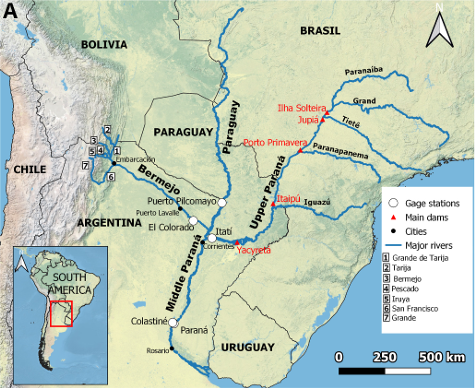
\includegraphics[width=0.65\linewidth]{figures/ch2/map rio parana.png}
    \caption{Rio Paraná Map}
    \label{fig:rio parana map}
\end{figure}

%\begin{figure}[H]
 %   \centering
  %  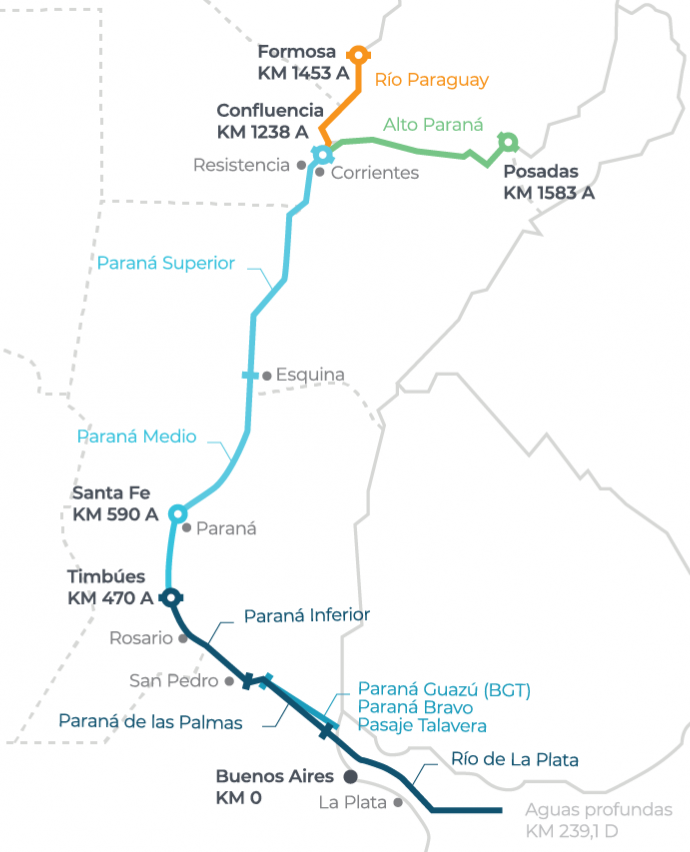
\includegraphics[width=0.5\linewidth]{figures/ch2/2025_mapa_vnt_extendida_tramos_profundidades_abril.png}
  %  \caption{The Vía Navegable Troncal (VNT) and the location of the Paraná and Paraná Guazú in it \autocite{agencianacionaldepuertosynavegacionNavegableTroncal2025}}
 %   \label{fig:VNT}
%\end{figure}

The Paraná river is formed by the junction of the rivers Grand and Paranaíba in south-central Brazil and flows for 4880 kilometers until it empties in the Río de la Plata near Buenos Aires, Argentina \autocite{orfeoHydraulicMorphologicalCharacteristics2002}. The river can be split up in three different sections: the upper, middle and lower Paraná. For these sections, the general characteristics related to discharge, channel size, and sediments are discussed.

The Upper Paraná River flows southwest, from the origin of the Paraná, until the confluence with the Paraguay river. Mean annual discharges at Porto São José, located near Porto Primavera at the confluence of the Paraná and Paranapanema in figure \ref{fig:rio parana map}, are between 6501 to 13,294 m³/s. The maximum flow velocity varies between 0.6–0.9 m/s in tributary channels and up to 1.4 m/s in the main channel during floods \autocite{stevauxUpperParanaRiver1994}. The Upper Paraná River exhibits a multi-channeled, braided pattern with numerous islands and sand bars, and its floodplain is strongly asymmetrical, being much wider on the right side (4.2–8.5 km) while the left margin erodes the Caiuá Formation \autocite{orfeoHydraulicMorphologicalCharacteristics2002}. During normal floods, water enters the floodplain through secondary and abandoned channels, producing slow and non-unidirectional flow, but extreme floods can cause crevasses and temporary channels. The channel is 1200–4500 m wide and 6–17 m deep with a slope of 0.096 m/km \autocite{stevauxUpperParanaRiver1994}. Finally, the suspended sediment concentration at Porto Rico, just South of Porto São José, equal 14.8×10(\textsuperscript{6}) tons/year and is mainly composed of quartz, mica, and kaolinite. The bed load at this location has a total discharge of 4.04×10$^6$ tons/year and consists of quartz-rich (95\%) medium to fine sand \autocite{stevauxUpperParanaRiver1994}.

After the confluence with the Paraguay river, the Upper Paraná goes over into the Middle Paraná River. This part of the river stretches until the start of the delta, just South of Rosario City. Near Corrientes City, South of the confluence, the mean annual discharge is 16,941 m³/s, with summer floods (Feb–Mar) and spring low water levels, reaching maximum values above 50,000 m³/s. The channel width ranges 1.9–4.7 km, with depths of 15–20 m and a slope of 0.085 m/km \autocite{orfeoHydraulicMorphologicalCharacteristics2002}. Below the Paraguay River confluence, suspended sediment concentrations are highly variable due to differences in discharge, confluence angle, and sediment characteristics between both rivers. The suspended solid concentration ranges from 18 to 554 mg/l, with the right margin showing much higher values (up to 1221 mg/l) than the left (maximum 88 mg/l)  \autocite{depetrisSuspendedLoadRio1968}. The suspended load is mainly silt (61–66\%) on the right margin and clay (79\%) on the left, with minor fine sand. The bed load is composed mostly of medium to fine quartz sand. The total sediment discharge is estimated at 158.4×10⁶ tons/year, with suspended load contributing 75\% of that \autocite{orfeoHydraulicMorphologicalCharacteristics2002}.

The final and smallest part of the Paraná is the Paraná delta, that ranges for around 320 kilometers, from Diamante, Entre Ríos, until the Río de la Plata near Buenos Aires. It is divided into three large regions: the Upper delta (from Diamante to Villa Constitución, Santa Fe province), the Middle delta (from Villa Constitución to Puerto Ibicuy, Entre Ríos province) and the Lower delta (from Puerto Ibicuy to the mouth of estuary called Río de la Plata). As mentioned in the introduction, this study focuses on the Lower delta specifically. Just upstream of the delta apex, near the city of Paraná, the mean annual discharge is 18,500 m³/s with peak discharges up to 60,000 m³/s \autocite{westerHydrodynamicModellingTidal2018}. Its width varies between 18 and 60 kilometres. The Paraná delta is characterized by many islands, which exist due to the large amounts of sediment that the Paraná delta carries: at its mouth it transports approximately a total of 160,000,000 tons of sediments per year. The particle load distribution is as follows: 25\% consists of clay, 60\% is silt and around 15\% can be characterized as sand \autocite{academialabParanaDelta}. This sediment is deposited in the joint Paraná and Uruguay estuary, the Río de la Plata.


%\section{Classification of Rio Paraná}
%Rivers can be described and classified in different ways. This classification can be linked to several factors such as age, colour or seasonality. 

%\subsection{The Age Classification of a River}
%Based on the development of the channel stage of a river, it can be labeled as youthful, mature or old age.  \autocite{davisGeographicalCycle1899}
%Applying this to the Rio Paraná makes it a complicated choice since the river is so long that it possesses features linked to each age label at distinct locations. therefore, it would be wiser to divide the Rio Paraná in three parts: upper, middle and lower Paraná. A youthful channel can be recognized through rapid flow, significant erosion, and a steep gradient. All these traits can be attributed to the upper Paraná zone.
%Moving on, a mature channel stage of river is in most cases a developed floodplain in the form of loops, called 'meander', and lateral erosion. This is mostly what can be seen in the middle part of the Paraná river.
%Lastly, the characteristics of an old age channel are comparable to the lower Paraná river. A wider floodplain, less rapid flow, and deltas. All of this is explained in \cite{orfeoParanaRiverArgentine2023}, and can be seen in the following Figure \ref{fig:rio parana map} from \cite{lopezweibelSourcesTemporalDynamics2022}.

%From Davis's study it follows logically that all these stages are represented in the total picture of the Paraná river since it is the ninth largest river in the world based on discharge \autocite{lopezweibelSourcesTemporalDynamics2022}.

%\subsection{The Colour Classification of a River}
%The colour of the river is also another label that can create a distinction. Based on two sets of papers/research  \autocite{furchWaterChemistryAmazon1984}, \autocite{sioliAmazonLimnologyLandscape1984}  Junk 1997, the water in rivers can be described as black, white or clear. The black water river is attributed to the 'leaching of tannins from decayed leaves of adjoining vegetated lands' \autocite{sand-mining-boek}, most common in Amazonia or in the United States. White waters on the other hand are, contrary to its qualification, usually brown coloured due to the high sediment concentration. Clear water rivers are located in environments with little to no erosion.
%Based on the theory and satellite imagery, one can again classify the Rio Paraná in different as a black and white river depending on the zone. The upper Paraná can be considered to be black due to its lack of sediment content, but rich in leaves content. But after the Bermejo river joins the Paraná, the river turns muddy all the way to the sea near Buenos Aires, as seen in Figure \ref{fig:confluences} \autocite{lopezweibelSourcesTemporalDynamics2022}.

\begin{comment}
    \begin{figure}[H]
    \centering
    \begin{subfigure}[b]{0.48\textwidth}
        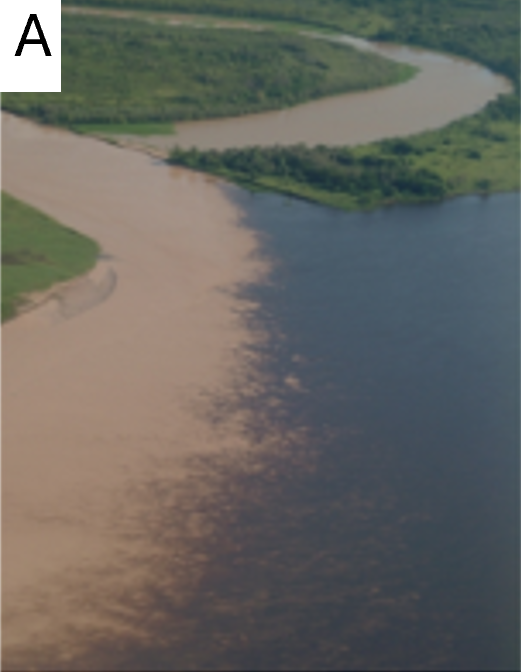
\includegraphics[width=\linewidth, height=5cm]{figures/ch2/Paraguay-Bermejo.png}
        \caption{Confluence of the Paraguay and Bermejo River}
        \label{fig:bermejo}
    \end{subfigure}
    \hfill
    \begin{subfigure}[b]{0.48\textwidth}
        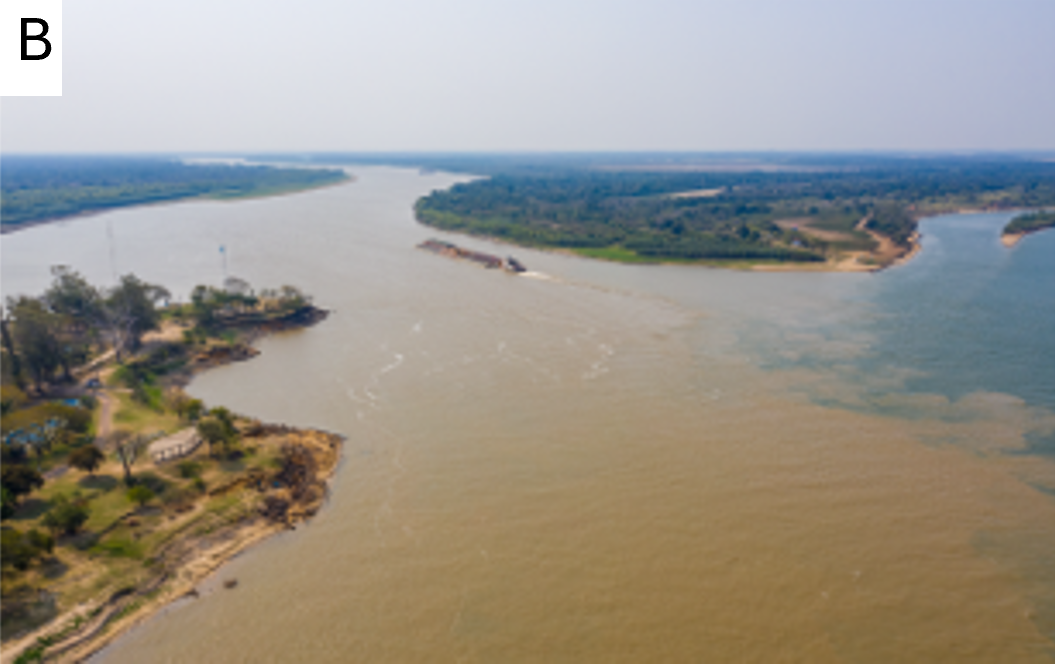
\includegraphics[width=\linewidth, height=5cm]{figures/ch2/Paraguay Parana.png}
        \caption{Confluence of the Paraguay and Paraná River}
        \label{fig:parana}
    \end{subfigure}
    \caption{Confluences of the Paraguay River with the Bermejo (left) and Paraná (right)}
    \label{fig:confluences}
    \end{figure}
\end{comment}


%\subsection{The Seasonal Flow of a River}
%The last classification relevant for this study is based on the flow characteristics and water availability. There are once again three types of categories: ephemeral, intermediate and perennial rivers. Ephemeral means that the river flow is not continuously present throughout the calendar year. Perennial rivers are the rivers whose flow is continuous and does not dry up during dry season, unlike the ephemeral rivers. Lastly the intermediate rivers are perennial rivers that dry up in extreme cases of drought.
%The Rio Paraná can be considered a perennial river due to its continuous flow over the years \autocite{furchWaterChemistryAmazon1984}, \autocite{sioliAmazonLimnologyLandscape1984}.

\section{Origin of sediment content in Paraná Guazú}
\label{sec:origin sediment content}
In the previous section, the quantities and distributions of sediment transport were lined out. However, a key step in constructing the sediment balance of the Paraná Guazú, located in the lower Paraná, is to identify the origin of its sediment. As shown in Figure \ref{fig:placeholder}, the lower and middle Paraná receive discharge from three main tributaries: the Bermejo, Paraguay, and Upper Paraná Rivers. The total average discharge in the middle Paraná is $18,389~\mathrm{m^3/s}$, of which 78\% is supplied by the upper Paraná. \citeauthor{lopezweibelSourcesTemporalDynamics2022} report that the Bermejo contributes only 2\% of this discharge. Nevertheless, the Bermejo is the dominant source of sediment, due to intense erosion in the Andes Eastern Mountain Range within its basin. During the wet season (November to April), multiple tributaries in the basin contribute large sediment flows, accumulating to an annual suspended sediment load of $106 ~\times 10^6$ t per year at El Colorado gauge station. 

It is interesting to know that the contribution of sediment from the Bermejo to the Paraná is approximately 90\% today, but that this is in fact due to the installation of the Itaipu dam built in 1971, located in the south of Brazil just before the border with Argentina and Paraguay. This modification of the sediment voyage cuts a supply of about 50\% compared the initial amount of sediment, this 90\% used to be 56\% of the sediment income before the construction of the dam. This explains us that the human action already hindered the initial inflow of sediment a long time ago \autocite{hibaParanaRiverEcological2024}.

In summary, while the Paraguay and Upper Paraná Rivers provide most of the fluvial discharge to the downstream delta, the Bermejo River delivers the majority of sediments \autocite{lopezweibelSourcesTemporalDynamics2022}. For this reason, the stretch of river beginning in the Bermejo basin and continuing via the Paraguay and middle Paraná to the Paraná Guazú is of particular importance in this study.  

\section{Types of sand mining}
In order to learn more about the effects that sand mining can cause, the general procedure of mining sand is of importance. Due to the need of sand in human society, various techniques have been established to get hold of sand. This can be done through so-called dry sand mining, where sand is won from the land, or through river sand mining. This study focuses on both, and for the river extraction, the focus lies on in-stream mining.

In-stream mining is the extraction of sand and gravel from the active channel of a river \autocite{sand-mining-boek}. A numer of types of in-stream dredging exist. Bar scalping or skimming is the most common extraction practice, consisting of removing the lower two thirds of a bar while leaving the top third to minimize alteration of the riverbed’s initial conditions. Dry pit channel mining involves creating a dry pit using mechanical or manual tools to extract sand or gravel; the remaining pits act as head cuts that modify upstream flow during high-water seasons. Wet pit channel mining, typically carried out in perennial rivers, produces similar effects and damages as the dry pit method. Bar excavation takes place downstream of a bar to capture sand and gravel being transported by the current. Finally, instream traps involve digging a hole to collect sediment during high flow periods, which can later be retrieved once water levels drop \autocite{sand-mining-boek}.

\section{The effects of river sand mining}
Existing literature provides a framework for possible effects that arise due to river sand mining. This framework helps with determining the exact effects of dredging in the Paraná delta.

As mentioned previously, rivers maintain an equilibrium between erosion, transport, and deposition of sediments. However, instream sand mining can discrupt this balance. This happens through direct disruption of the channel geometry or through so-called incision and related undercutting of banks \autocite{sand-mining-boek}. The direct disruption of the river bed depends on the type of sand mining technique employed. In the case of pit excavation, the river bed is locally lowered and a so-called 'nick point' is created. With bar skimming the river bed is widened \autocite{sand-mining-boek}. For the remainder of this section, the consequent effects of the local river bed lowering (the nick point) are discussed.

Channel incision causes the nick point to migrate both upstream and downstream. In the case of high flows, due to its shape, the nick point is the point where most erosion occurs. Water plunges over the step and erodes the bed at the base. As flows continue, the drop migrates upstream, a process which is often called head-cutting in literature. On the other hand, a process called 'hungry water' causes downstream migration of the pit \autocite{sand-mining-boek}. At the mining pit the water level is deeper, which causes the flow velocity to reduce locally. This leads to a decrease in flow energy and thus to more deposited sediment. When the flow leaves the mining area, water levels are shallower again meaning that flow velocity and energy significantly increase. A lot of sediment has been deposited in the nick point, meaning that the water is not using its full sediment carrying capacity anymore. In other words, the water is 'hungry' for sediment and erosion downstream increases \autocite{sand-mining-boek}. 

Through the combined effects of head-cutting and hungry water, the mining pit can extend beyond the initial dimensions caused by direct disruption. This happens in both downstream and upstream directions, as summarized in figure \ref{fig:channelbedeffects}. \textcite{hackneyRiverBankInstability2020} have demonstrated that sand mining has the potential to lower bed levels sufficiently to
cause river bank instability.

\begin{figure}[H]
    \centering
    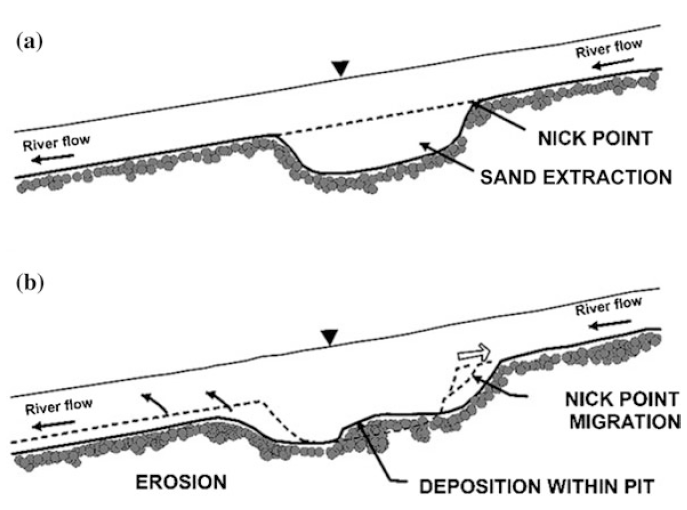
\includegraphics[width=0.75\linewidth]{figures/channelbedeffects.png}
    \caption{a: direct disruption leads to a locally lowered water bed, b: channel incision makes the pit migrate upstream through head cutting and downstream through 'hungry' water \autocite{sand-mining-boek}}
    \label{fig:channelbedeffects}
\end{figure}

Previous studies have shown that bed coarsening can also occur as a result of sand-mining. Fine particles are removed, leading to a greater concentration of coarse (gravelly) particles. This effect can also be seen upstream \autocite{sand-mining-boek}. Further, sand mining can lead to changes in both water quality and quantity. The process of dredging the fine sand stirs fine organic and inorganic particles, thereby increasing the turbidity of the water. This reduces light penetration, which means less photosynthesis and ultimately less organic growth in the water \autocite{sharipEffectsSeasonSand2014}.

As mentioned before, mining pits are often places with significant deposition of particles. Fine, nutrient-rich particles can settle and get trapped in the pits. This then reduces the transport of nutrients from the river to the coastal waters \autocite{sand-mining-boek}.

Concerning the water quantity, the most relevant effects are related to the groundwater: the lowering of the river bed through direct disruption or channel incision can lead to a lower groundwater table. This can lead to settlements or have negative effects on flora and fauna surrounding the river \autocite{rentierEnvironmentalImpactsRiver2022}.

Finally, it must be noted that the effects of sand mining can be diverse: previous studies have shown negative impacts on biodiversity, including reduced benthic fauna, disrupted fish spawning habitats, and depletion of natural mosquito predators such as dragonflies \autocite{sand-mining-boek}. The socioeconomic effects of mining can vary, in the short-term it often provides employment, income, and government revenue through royalties and taxation. However, in the long-term the operation can cause a reduction in access to clean water and can cause water scracity, especially in dry periods. Additionally, loss of land and access to land together with loss of trees and vegetation can jeopardize the local food security. Finally, infrastructure can be damaged by the lowering of the river bed and/or the groundwater table \autocite{sand-mining-boek}.




NBS context

The Paraná Delta, the end of the Paraná-Paraguay river wetland system, begins in the city of Diamante in Entre Ríos province. It stretches for 300 kilometres and covers some 2.3 million hectares. Dotted with islands, these wetlands are a source of ecosystem services such as flood and drought buffering, water purification, erosion control and coastal protection, climate regulation, as well as the provision of shelter, feeding and breeding sites for various wildlife species. It also provides resources including fish, foraging, timber, medicine, and materials for construction and clothing \autocite{hibaParanaRiverEcological2024}.

In recent years, wetlands have become increasingly important for another key reason: their role as allies against climate change. They improve the resilience of communities to its impacts, serve as natural barriers against floods and droughts, and also function as carbon sinks. Despite playing these important roles, these ecosystems remain under great threat from human action – it is estimated that globally, 85 percent of the wetlands that existed three centuries ago have been destroyed or drastically transformed \autocite{hibaParanaRiverEcological2024}.


NBS definitie

A general definition of Nature-based solutions:

\textit{“A set of actions to protect, conserve, restore, sustainably
use and manage natural or modified terrestrial, freshwater, coastal and marine
ecosystems, which address social, economic and environmental challenges
effectively and adaptively, while simultaneously providing human well-being,
ecosystem services, resilience and biodiversity benefits” \autocite{eiselinVerenigdeNatiesStemmen2022}}

7 GOals?

\begin{figure}[H]
    \centering
    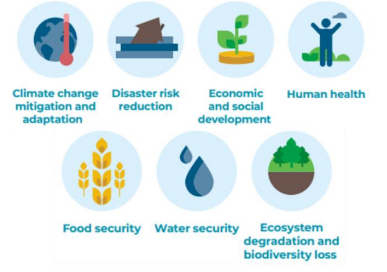
\includegraphics[width=0.50\linewidth]{figures/ThesevenNBSgoals.png}
    \caption{Seven goals for achieving a good NBS \autocite{dunlopEvolutionFutureResearch}}
    \label{fig:7g}
\end{figure}

\chapter{Methodology}
\label{chap:methodology}

This chapter captures all methods used to answer the research questions. It describes the collection of data through various sources, such as publicly available time series and field data that were recorded in this particular study. With these data, models were made, which were used for answering the sub-questions which lead to answering the main research question.

\section{Analysis of existing data sets}
\label{sec:desk study}
In order to analyse and draw conclusions about the situation, the data sets used are explained in the following paragraphs. A summary is provided in Table \ref{tab:data collection summary}.

The first source of data was the Instituto Nacional del Agua (INA). Since collaboration between TU Delft and INA is a central aim of this study, an “our data is your data” policy was applied, under which data were openly exchanged. Through this approach, INA provided a large number of datasets, which are presented in Table \ref{tab:data collection summary}. In addition, background knowledge about water discharge, erosion and negative impacts was shared in the form of publications and reports produced by INA staff and contacts. Furthermore, INA supplied geospatial datasets, including bathymetric surveys and a Digital Elevation Model (DEM) of the study area.

INA also provided a number of public sources for further hydrodynamic analysis and GIS applications. These included flow data from multiple gauging stations and publicly available bathymetric datasets. Examples are the Sistema Nacional de Información Hídrica (SNIH), point-based water level measurements from the governmental department Alerta, and water level records from the Prefectura Naval Argentina (PNA). An overview of these datasets is provided in Table \ref{tab:data collection summary}.
Finally, additional data were obtained through other stakeholder contacts. For example, the Dutch Embassy provided a case study on Nature-based solutions (NbS) for the Paraguay River. More information on the approach with stakeholders can be found in Section \ref{sec:stakeholder methods}.

\begin{table}[H]
    \centering
    \renewcommand{\arraystretch}{1.2} % row spacing
    \setlength{\tabcolsep}{4pt}
    \caption{Summary of data sources}% column padding
    \begin{tabularx}{\textwidth}{p{3.5cm}p{8cm}p{3.5cm}}
        \toprule
        Name & Description of data type & Source \\
        \midrule
        Comparative studies  & Background literature on geomorphology of similar areas & INA   \\
        INA Dataviewer         & Historical observations and simulations of water level and discharge time series & INA  \\
        DEM of lower Paraná & GeoTIFF file containing a Digital Elevation Model of the study area & INA \\
        Bathymetry (GIS) & Results from field campaigns in and around study area (2011, 2015, 2018) & INA \\
        Sand extraction permits & Agreements on locations and volumes of dredged sand & INA \\
        MarineTraffic & Live AIS vessel data & \cite{marinetraffic2025} \\
        Prefectura Naval Argentina  & Water level measurements & \cite{prefecturanaval2025} \\
        SNIH & Water level, discharge, fine and course sediment concentration & \cite{snih2025} \\
        AquaMonitor & Deltares tool that represents water gains and losses based on historical satellite imagery & \cite{aquaMonitor2025} \\
        Bathymetry (pdf) & Detailed bathymetries along Paraná river in pdf-format & \cite{agencianacionaldepuertosynavegacionNavegableTroncal2025} \\
        Google Earth & Satellite imagery of the globe. Can be used for a chosen time period of 1984-now & \cite{googleearth2025}  \\
        \bottomrule
    \end{tabularx}
    \label{tab:data collection summary}
\end{table}

\subsection{SNIH measurement stations}
\label{sec:measurementstations}
The measurement stations from the SNIH that were used for the data collection are discussed in this section. In order to have accurate estimations of the sediment content in the Lower Paraná, it is interesting to consider its origin. As discussed in Section \ref{sec:origin sediment content}, most of the sediments in the Middle Paraná originate from the Bermejo river in northern Argentina. A representative measurement station for this river is found near El Colorado, Formosa province. Here, the SNIH reports long series of measurements of water elevation, discharge and sediment concentrations.

Moving downstream, the Bermejo confluences with the Paraguay river. Merely 80 kilometers further downstream, the confluence of the Paraguay and Paraná river is located, near the city of Corrientes. Here, a drastic change in fluvial discharge occurs. Therefore, a station that represents the flow in the Middle Paraná was sought. Approximately 500 kilometers downstream of the confluence, the Túnel subfluvial station near Santa Fe provides data. See Figure \ref{fig:rio parana map} for the location of El Colorado and Paraná (near Santa Fe). 

As explained in Chapter \ref{chapter:background}, the two main tributaries of the Paraná that later flow into the Río de la Plata are the Paraná de las Palmas and the Paraná Guazú. To examine the distribution of discharge and sediment concentrations over these tributaries, two stations were selected and are shown in Figure \ref{fig:flow partition}. First, the Zárate station was considered on the Paraná de las Palmas. On the Paraná Guazú, the Brazo Largo station was selected for data analysis. Table \ref{tab:stations data collection} presents the data for all stations considered. Note that every dataset contains measurements of water level, discharge, fine sediment concentration and course sediment concentration. Most of the data is measured monthly, however some information is recorded on shorter time intervals. 

\begin{figure}[H]
    \centering
    \includegraphics[width=0.75\linewidth]{figures/ch4/Flow partition1.png}
    \caption{Measurement stations of interest on Paraná de las Palmas and Paraná Guazú (\cite{googleearth2025})}
    \label{fig:flow partition}
\end{figure}

\begin{table}[H]
    \centering
    \renewcommand{\arraystretch}{1.2} % extra row spacing
    \setlength{\tabcolsep}{8pt}       % extra column spacing
    \caption{Selection of SNIH measurement stations}
    \begin{tabular}{lllc}
        \toprule
        Station & SNIH ID & River & Data availability \\
        \midrule
        El Colorado         & 2602 & Bermejo               & 1968--2025 \\
        Túnel Subfluvial    & 3050 & Middle Paraná         & 1983--2025 \\
        Zárate              & 4001 & Paraná de las Palmas  & 1993--2025 \\
        Brazo Largo         & 4002 & Paraná Guazú          & 1993--2025 \\
        \bottomrule
    \end{tabular}
    
    \label{tab:stations data collection}
\end{table}

\subsection{Sand mining quantities}
The number of vessels involved in river dredging activities on the Paraná Guazú was determined using AIS (Automatic Identification System) data. Vessel movements between dredging sites and ports were monitored through MarineTraffic. Although historical records were not considered, the daily activity observed during the study period provided an estimate of the sand extraction volumes. 

Alternatively, a collection of dredging permits in the river was considered. To avoid adverse impacts on the hydraulic regime of the river due to dredging, companies must first obtain permits from the \textit{National Water Institute} (INA). These permits specify the locations and volumes of the proposed dredging activities. The information they provide serves as a reliable estimate of the total material being removed from the river, thereby influencing the sediment balance. Therefore, the permits were analysed for the area of interest.
Subsequently, the information gathered from AIS data and extraction permits were combined, resulting in estimates of volumes that are dredged in the study area. In addition, conversations with stakeholders provided insights and made a comparison with the results of the data collection possible.

The information about dry sand mining was gained through different sources. The main sources were a literature review and the semi-structured interviews, which are explained Section \ref{sec:stakeholder methods}. These were used to gather data on dry sand mining quantities, usage purposes, and the factors influencing demand for sand from the region. The literature review provided background and quantitative information, while interviews offered insights from stakeholders directly involved in sand extraction and use in the study area.

\section{Field study}
\label{sec:field study}
The goal of the fieldwork was to obtain data from measurements on the boat using different devices, as well as obtaining resourceful information from chosen stakeholders in the area of the fieldwork. This data would then be filtered and analyse to help support conclusions.

\subsection{Stakeholders}
\label{sec:stakeholder methods}
In this study, a qualitative research was carried out to explore perceptions and experiences related to sand extraction in the lower delta area. For this, interviews were conducted to capture insights from participants with diverse perspectives.

A qualitative approach was chosen because it allows for a detailed understanding of participant's views and interpretations. This design is particularly suited to capture the complexity of social and environmental issues and to highlight the ways in which different stakeholders experience the delta region and the activities related to it. Data were collected through semi-structured interviews, a method that combines prepared guiding questions with the flexibility to follow up on unexpected but relevant topics raised by participants. This format ensured that key themes were consistently addressed in interviews while also allowing interviewees to elaborate on issues they considered important. In practice, a topic guide with questions per stakeholder was developed to provide structure, but the interviewer encouraged open-ended responses and probed further where clarification or depth was needed. During the interview, responses were written down in key words. The prepared questions for specific stakeholders as well as their unprocessed responses are given in Appendix \ref{chap:interviews}.

In case of language barriers, the questions and responses were translated to English by INA staff members. Most stakeholders were approached by email to get in contact or were reached on-site. After each interview, permission was asked to quote and name the stakeholder in the report. Table \ref{tab:stakeholders} gives an overview of stakeholders who were contacted, when and by which method. 

\begin{table}[H]
    \centering
    \caption{Overview of stakeholder approach}
    \begin{tabularx}{\textwidth}{l l l}
        \toprule
        Date & Occupation & Method \\
        \midrule
        12-09-2025 & Fishers & Email \\
        12-09-2025 & Ports & Email \\
        12-09-2025 & Filmmakers & Whatsapp \\
        24-09-2025 & Landowners & Whatsapp and On-site \\
        25-09-2025 & Agencia Nacional de Puertos y Navegación (ANPYN) &  Email \\
        25-09-2025 & Dredgers & On-site \\
        25-09-2025 & Camping owner & Email and On-site \\
        30-09-2025 & Prefectura Naval Argentina (PNA) & Email \\
        \bottomrule
    \end{tabularx}
    
    \label{tab:stakeholders}
\end{table}

% TABEL AANPASSEN. WIE HOE WANNER. LOCATION AND LANGUAGE NAAR DE RESULTATEN. OOK DE BENAMING SPECIFIEK IN DE RESULTATEN BENOEMEN EN HIER ALGEMEEN BLIJVEN. EXTRA KOLOM HOE TEOVOEGEN; Email, WHATSAPP, TEAMS

\subsection{Measurement variables and equipment}
\label{Measurement variables and equipment}
In this section, the types of measurements are explained as well as the locations of measurements taken. The goal of the fieldwork was to obtain data from critical sections in the study area, specifically those sections that were deemed critical for establishing the sediment balance. Two important locations in the study area are the confluence from the Ibicuy and Paraná Guazú, and that of the Paraná Guazú and Talabera. In these sections, sediment samples and flow measurements were recorded. Once this data was gathered, it was analysed and compared to previously obtained data to draw conclusions. 

% \begin{figure}[H]
%     \centering
%     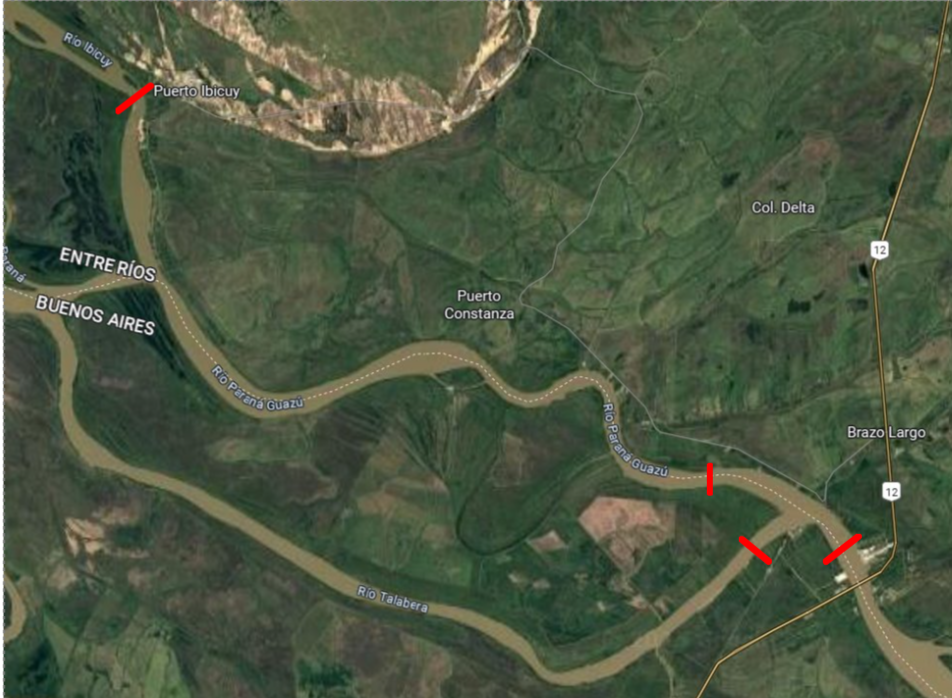
\includegraphics[width=0.5\linewidth]{figures/ch4/Critical measurement points.png}
%     \caption{Critical Cross Section Measurements}
%     \label{fig:fieldwork cross sections}
% \end{figure}

% The program of the boat days consisted of going over the indicated critical cross sections (in red on Figure 4.2) a total of 4 times, using the equipment of INA to save the necessary information of the river. 

The first measured type of data is the flow velocity profile of the river. This was recorded by a SonTek RiverSurveyor M9 Acoustic Doppler Current Profiler (ADCP). This device consists of two components both placed on a floating board held next to the boat while advancing. The components are a vertical acoustic echo sounder beam placed on the back end of the floating board, and a rectangle shape box containing a microprocessor that computes the data on the front end of the board, as seen in Figure \ref{fig:SonTekmeasurement}.

\begin{figure}[H]
    \centering
    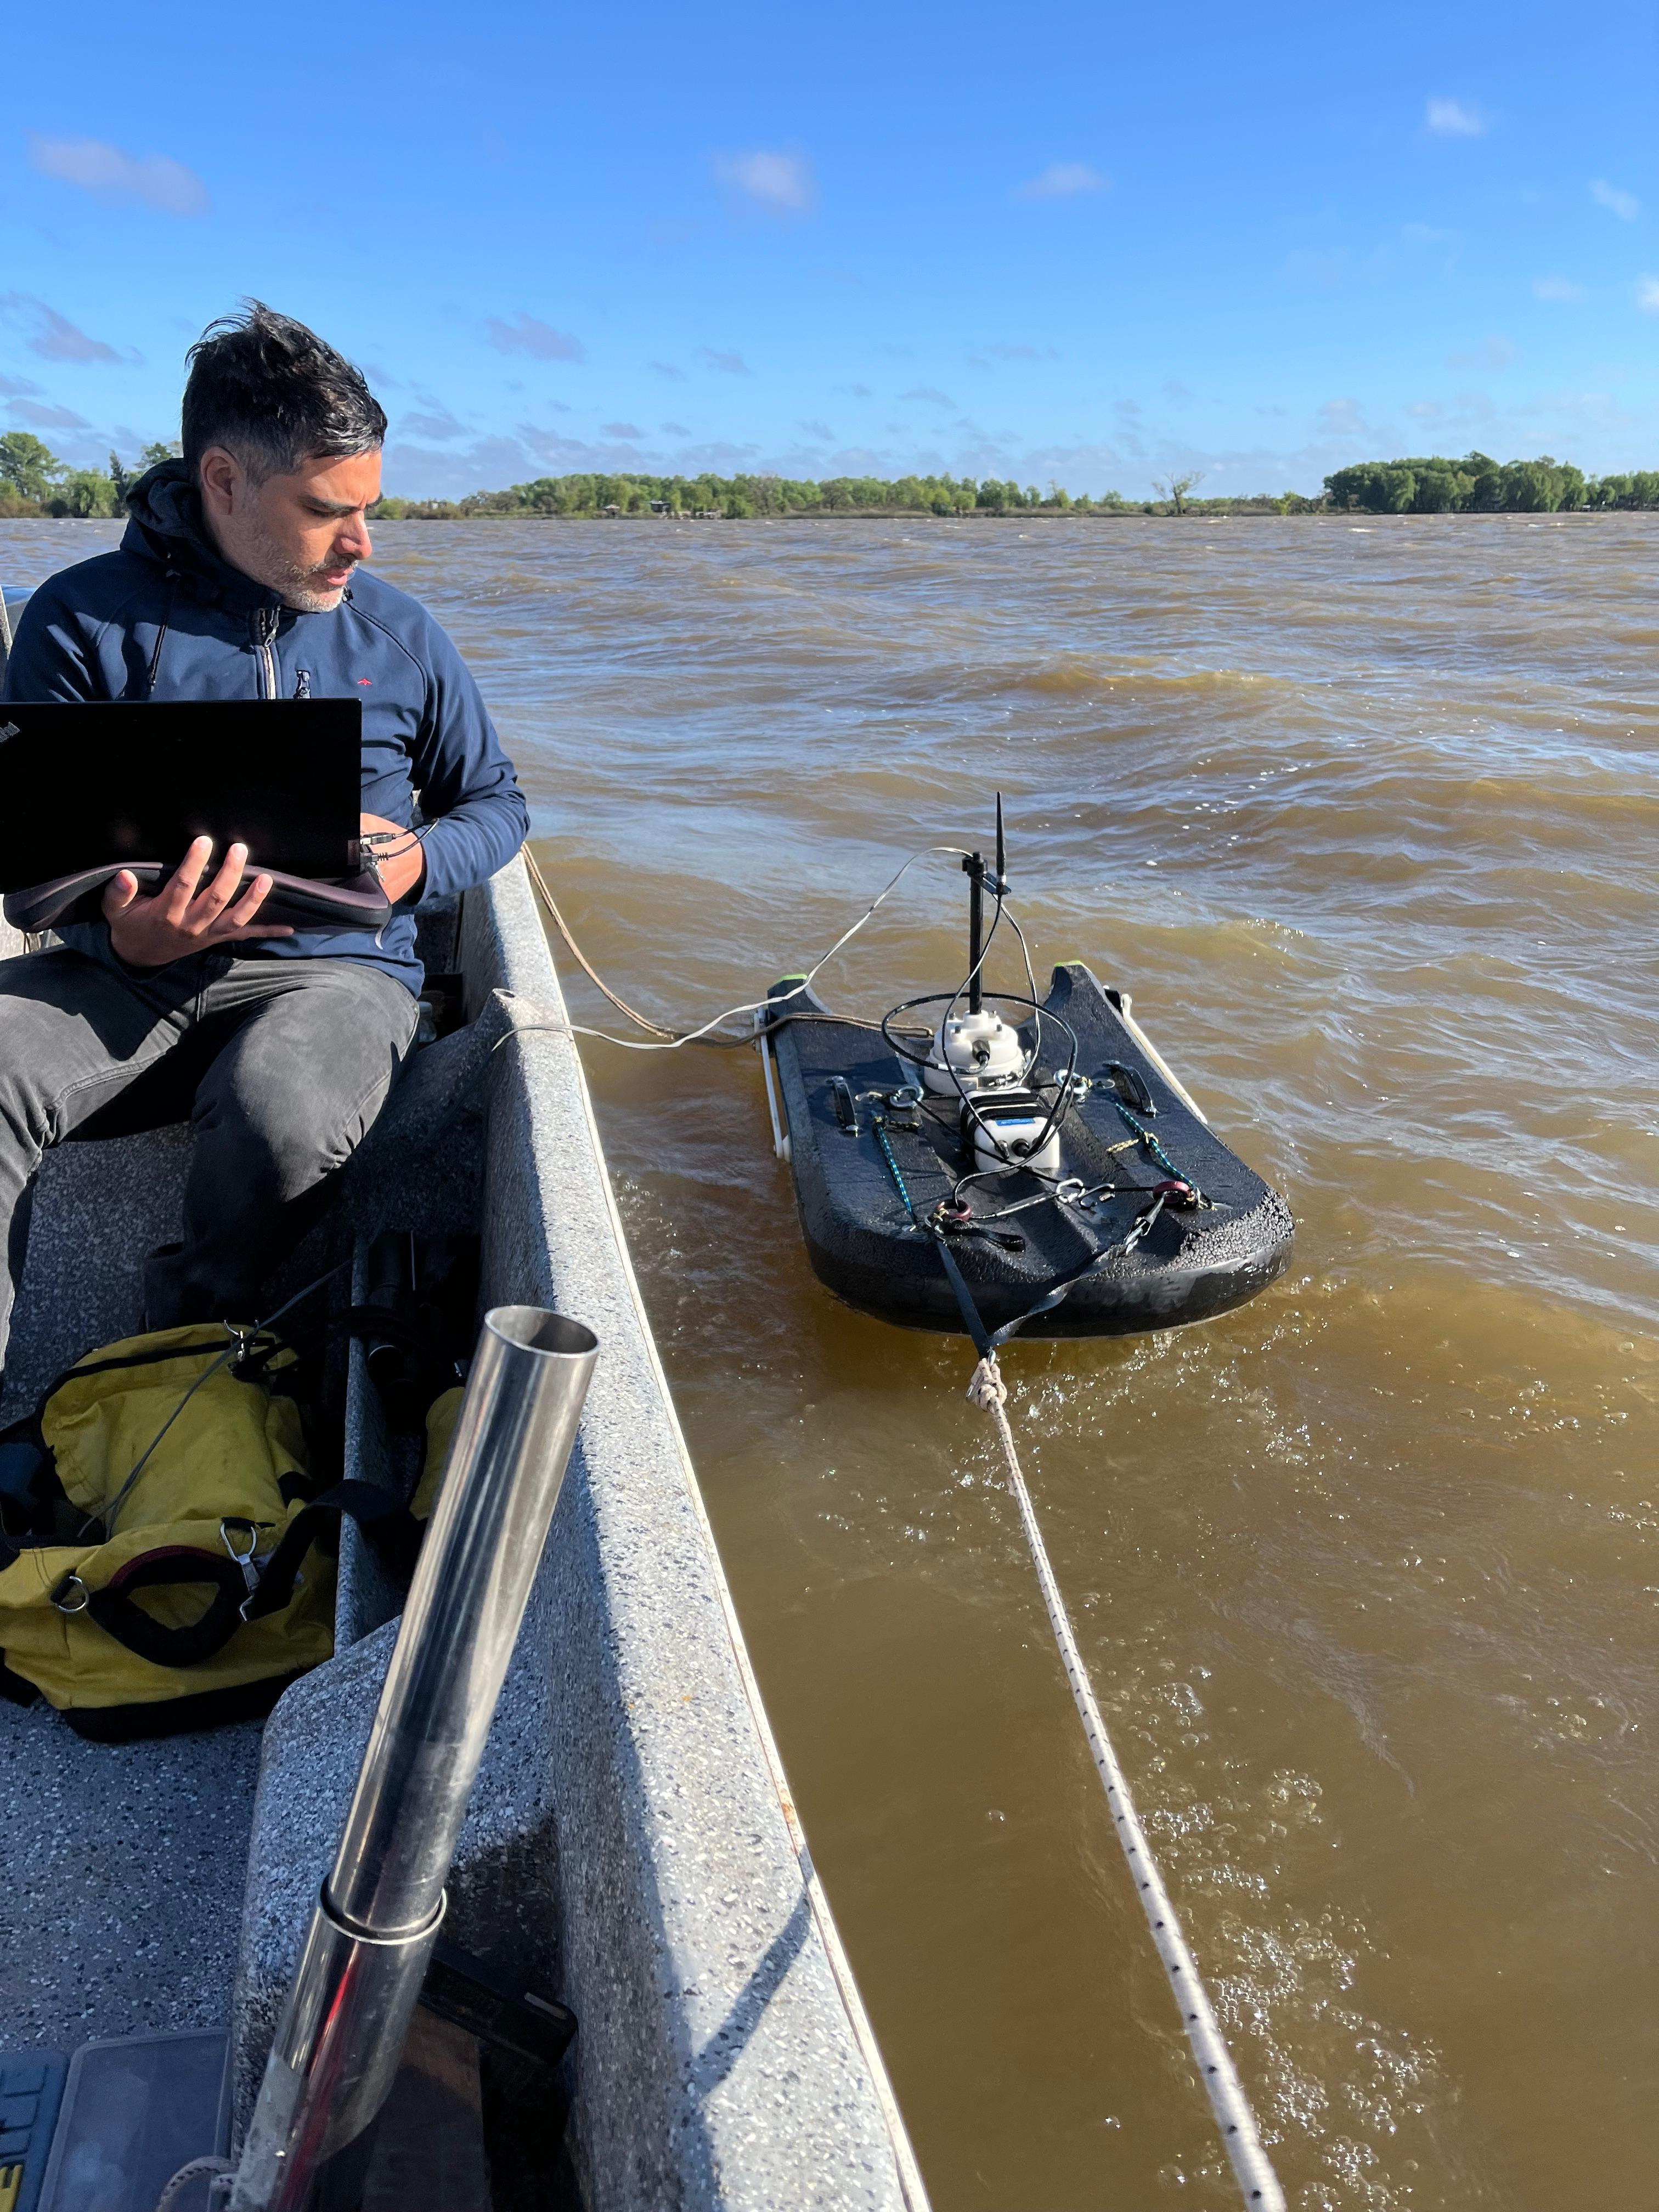
\includegraphics[width=0.5\linewidth]{figures/ch4/sonteknico.jpg}
    \caption{SonTek M9 installed in the field}
    \label{fig:SonTekmeasurement}
\end{figure}

The speciality of the SonTek M9 is that it uses multiple acoustic frequencies to find a high resolution range of depths and flow velocities, while still tracking the geo-referenced position of the vessel using GNSS \autocite{xylemSonTekM9}. The flow velocity is expressed in the form of a vector and the significance of this data lies in the fact that flow velocity is needed to compute the discharge.

Secondly, the bathymetry, the depth of a channel at the position of the boat on a given timestep, was recorded by using two different methods: the ADCP and the Garmin echosounder. Moving over the whole width of the channel yielded a longitudinal profile, indicating what depth lies at what coordinate.
The echosounder was attached to a pole on the side of the boat, and dipped into the water while the boat was moving. This pole was connected to the Garmin screen showing depth and bathymetry of the channel, as can be seen in Figure \ref{fig:Garmin}. In addition, this screen allowed for monitoring of possible disruption of the river bed. The profile was taken on the whole trajectory between Puerto Guazú to Ibicuy in both upstream and downstream directions. The profile is shown in Figure \ref{fig:measurements day2}.

\begin{figure}[H]
    \centering
    \begin{subfigure}[b]{0.48\textwidth}
        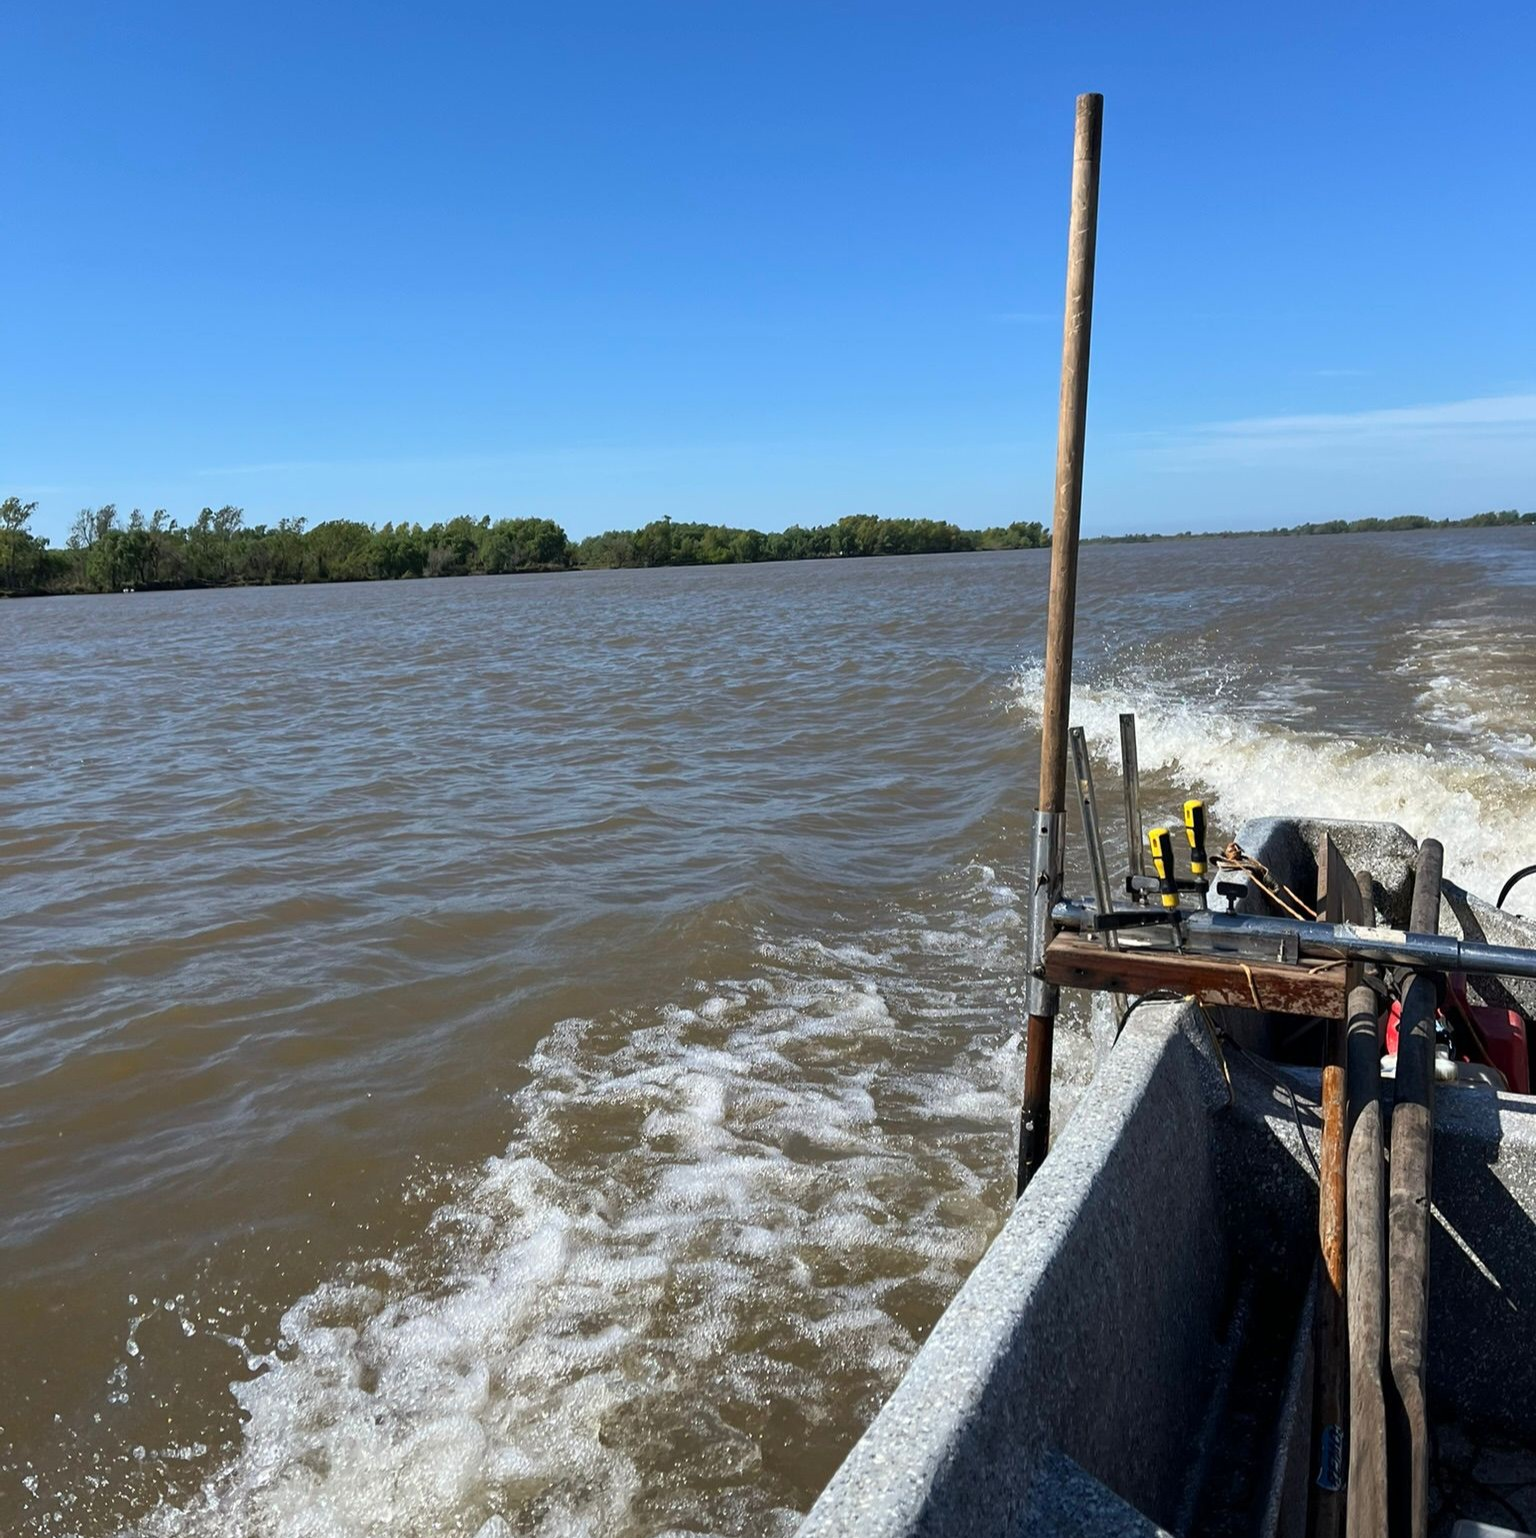
\includegraphics[width=\linewidth]{figures/ch4/Echosounder.jpg}
        \caption{Echosounder attached to boat}
        
    \end{subfigure}
    \hfill
    \begin{subfigure}[b]{0.48\textwidth}
        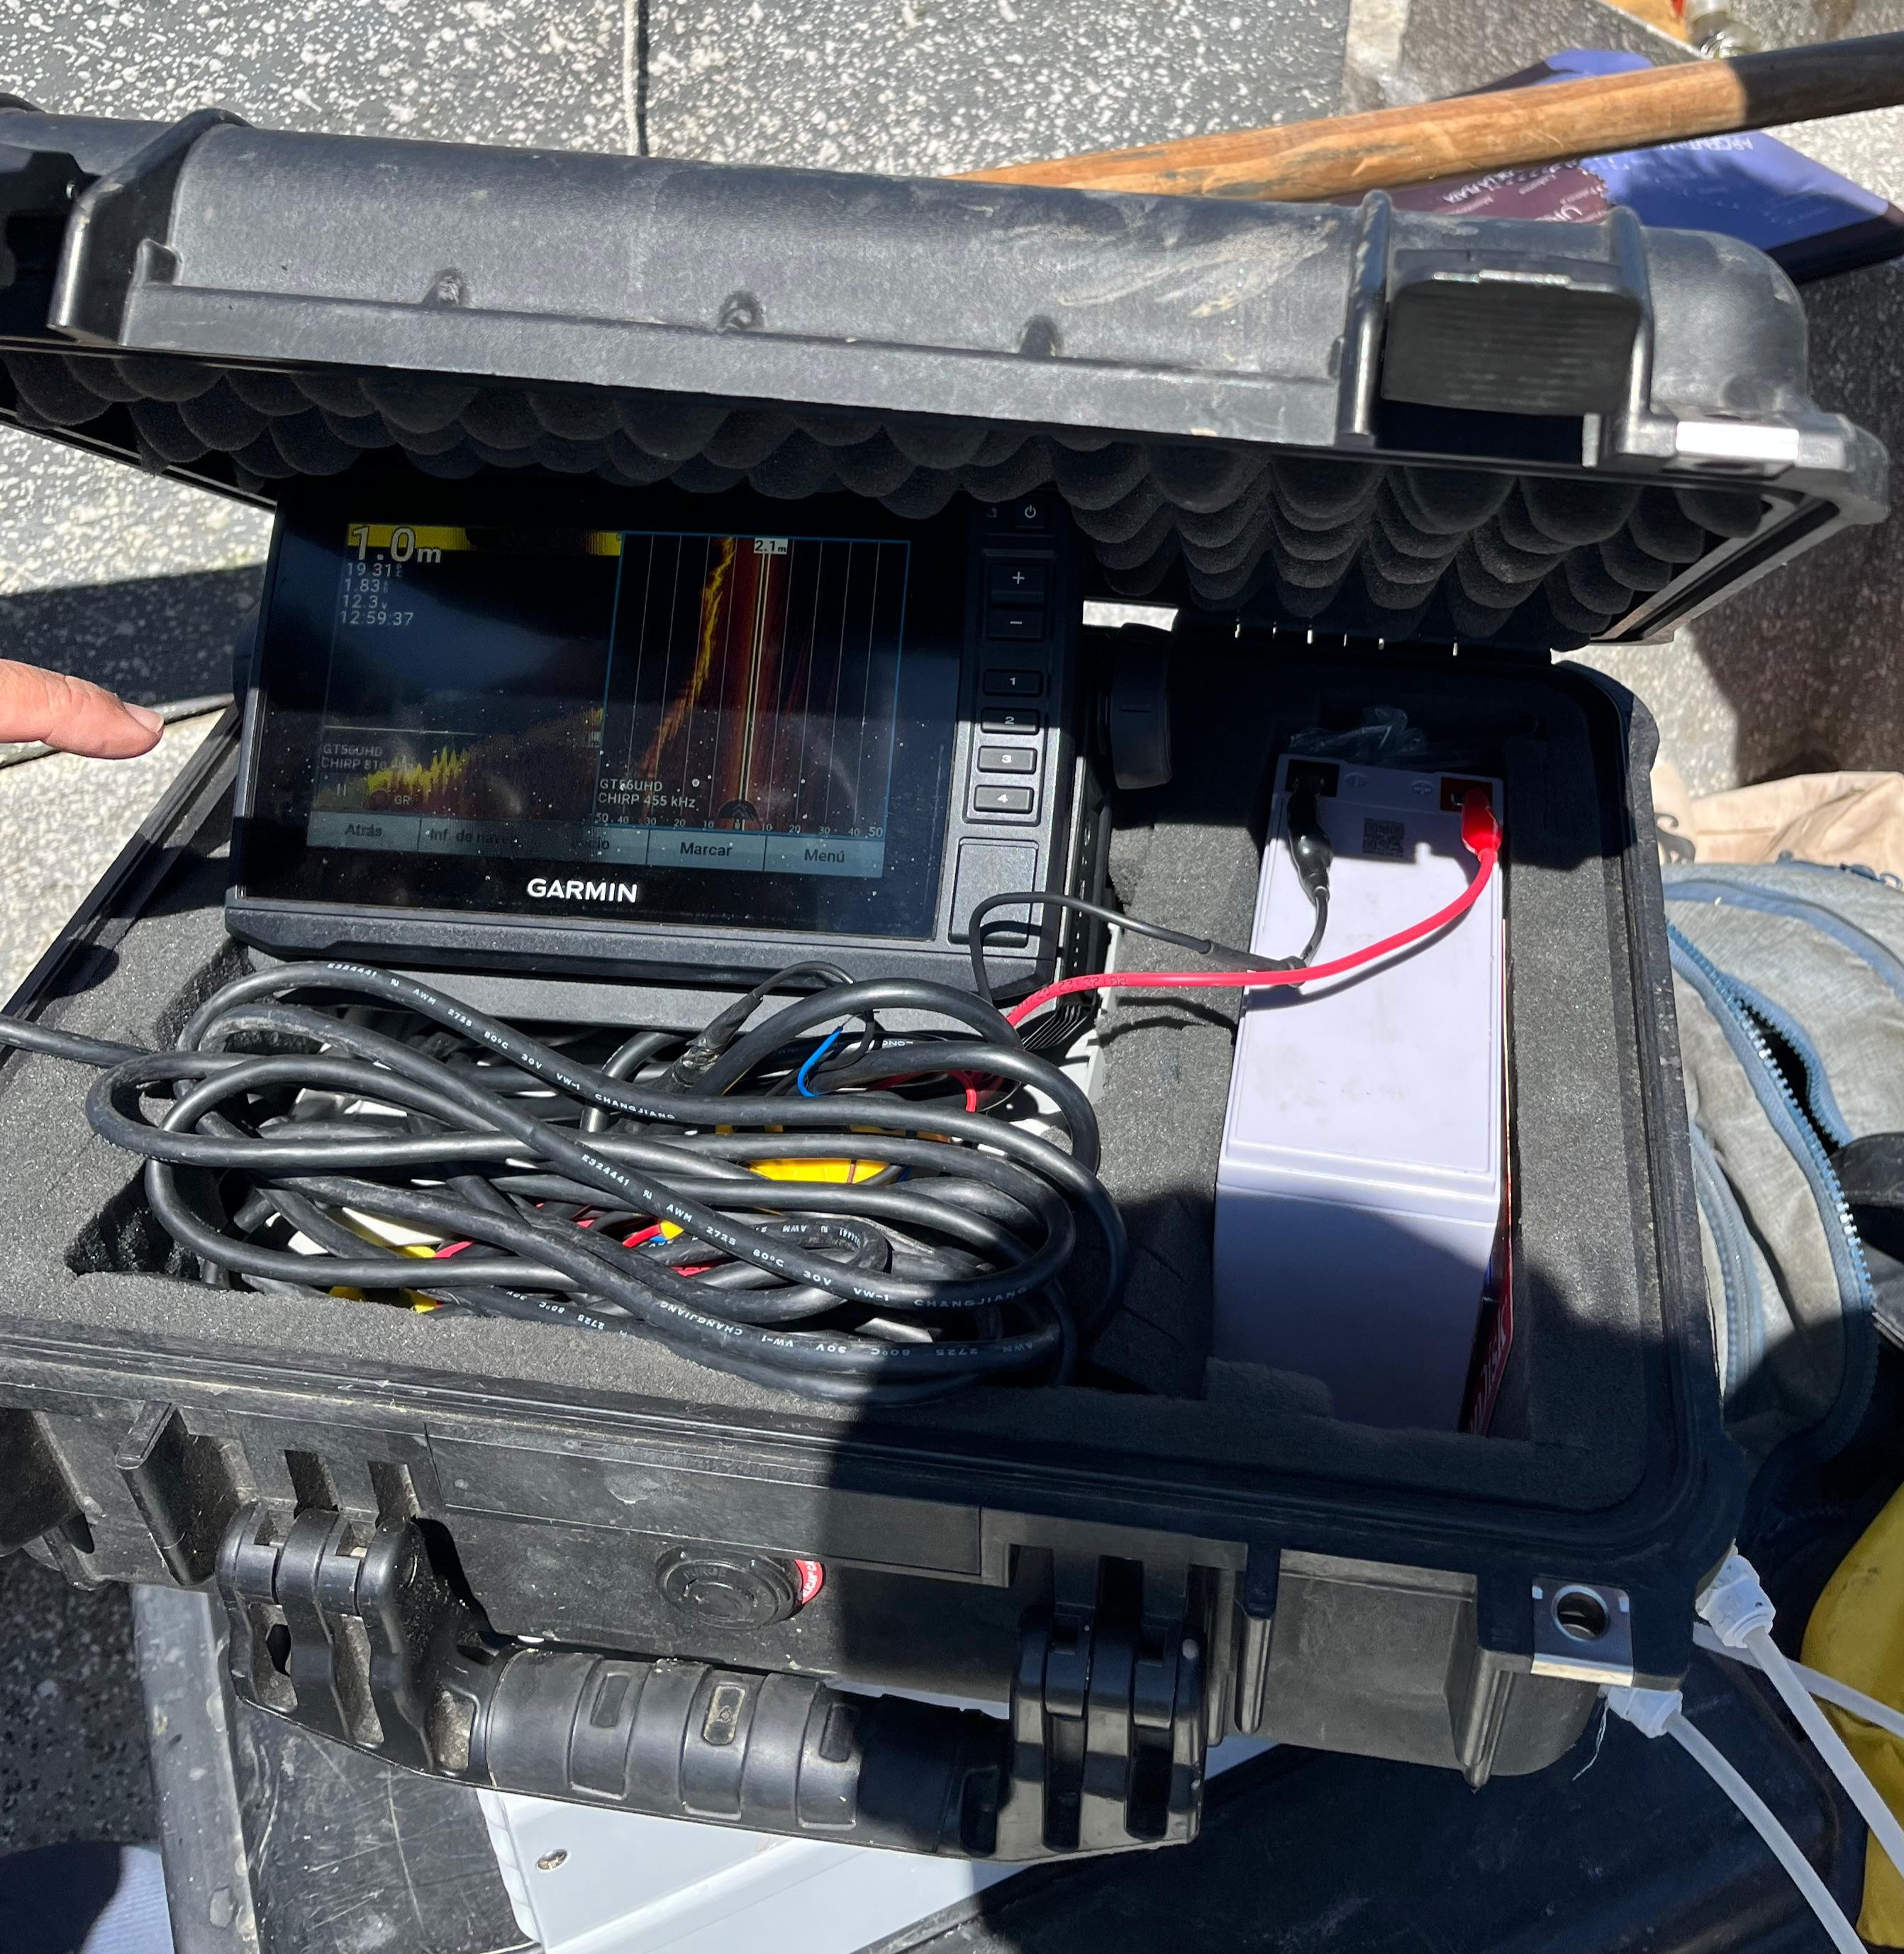
\includegraphics[width=\linewidth]{figures/ch4/garmin.jpg}
        \caption{Garmin material}
        
    \end{subfigure}
    \caption{Echosounder and Garmin measurements}
    \label{fig:Garmin}
\end{figure}

From the bathymetry and flow velocity, the discharge can be determined. The flow velocity \(\mathbf{v}\) was integrated over the depth and width of the channel (through a cross-section) which in the end yielded the discharge. Equation \ref{eq:discharge_integration} summarizes this procedure.

\begin{equation}
    Q = \iint_A \mathbf{v} \cdot d\mathbf{A}
    \label{eq:discharge_integration}
\end{equation}

\noindent Where:
\begin{itemize}
    \item \(Q\) is the discharge, cubic meters per second [m\textsuperscript{3}/s];
    \item \(\mathbf{v}\) is the flow velocity vector, meters per second [m/s];
    \item \(A\) is the cross-sectional area perpendicular to the flow, square meters [m\textsuperscript{2}];
    \item \(d\mathbf{A}\) is an infinitesimal area element.
\end{itemize}

The number of required measurements of a single cross section was defined by the variability of the measurements. That is, a minimum of two measurements was carried out, which was deemed to suffice when the second discharge measurement fell within 10\% of the first one. In addition, correct operation of the vessel's velocity was essential for reliable discharge results: it was made sure that the boat speed never exceeded the flow velocity perpendicular to the cross section under consideration. 

% The aim of the fieldwork was to obtain the data of flow velocity and discharge at the three critical points around the bifurcation of interest during different times, one in the morning and in the afternoon. Consequently this would indicate some changes in discharge for different times, flows, circumstances hence solidifying our data base of examples. 

Further, data was gathered on the suspended sediment concentration of the river. This was done by collecting water with the help of an APEMA BS6A peristaltic pump connected to two plastic tubes. The first tube was short and was used to insert water into the plastic bottles on the boat. The second, long, tube was connected to a weight, which could be lowered into the river until a certain depth. At the desired depth, the fluid was pumped to the surface and collected in the plastic bottles. Then, samples were sealed in order to be sent to the water quality lab in the hydraulic section on the INA site, as seen in Figure \ref{fig:suspended-sediment}. Here, concentrations of fine sediments were determined for all samples. The evolution of the concentrations along the study area is studied in Chapter \ref{chap:hydroanalysis}.

\begin{figure}[H]
    \centering
    % Left image
    \begin{subfigure}[t]{0.48\textwidth}
        \centering
        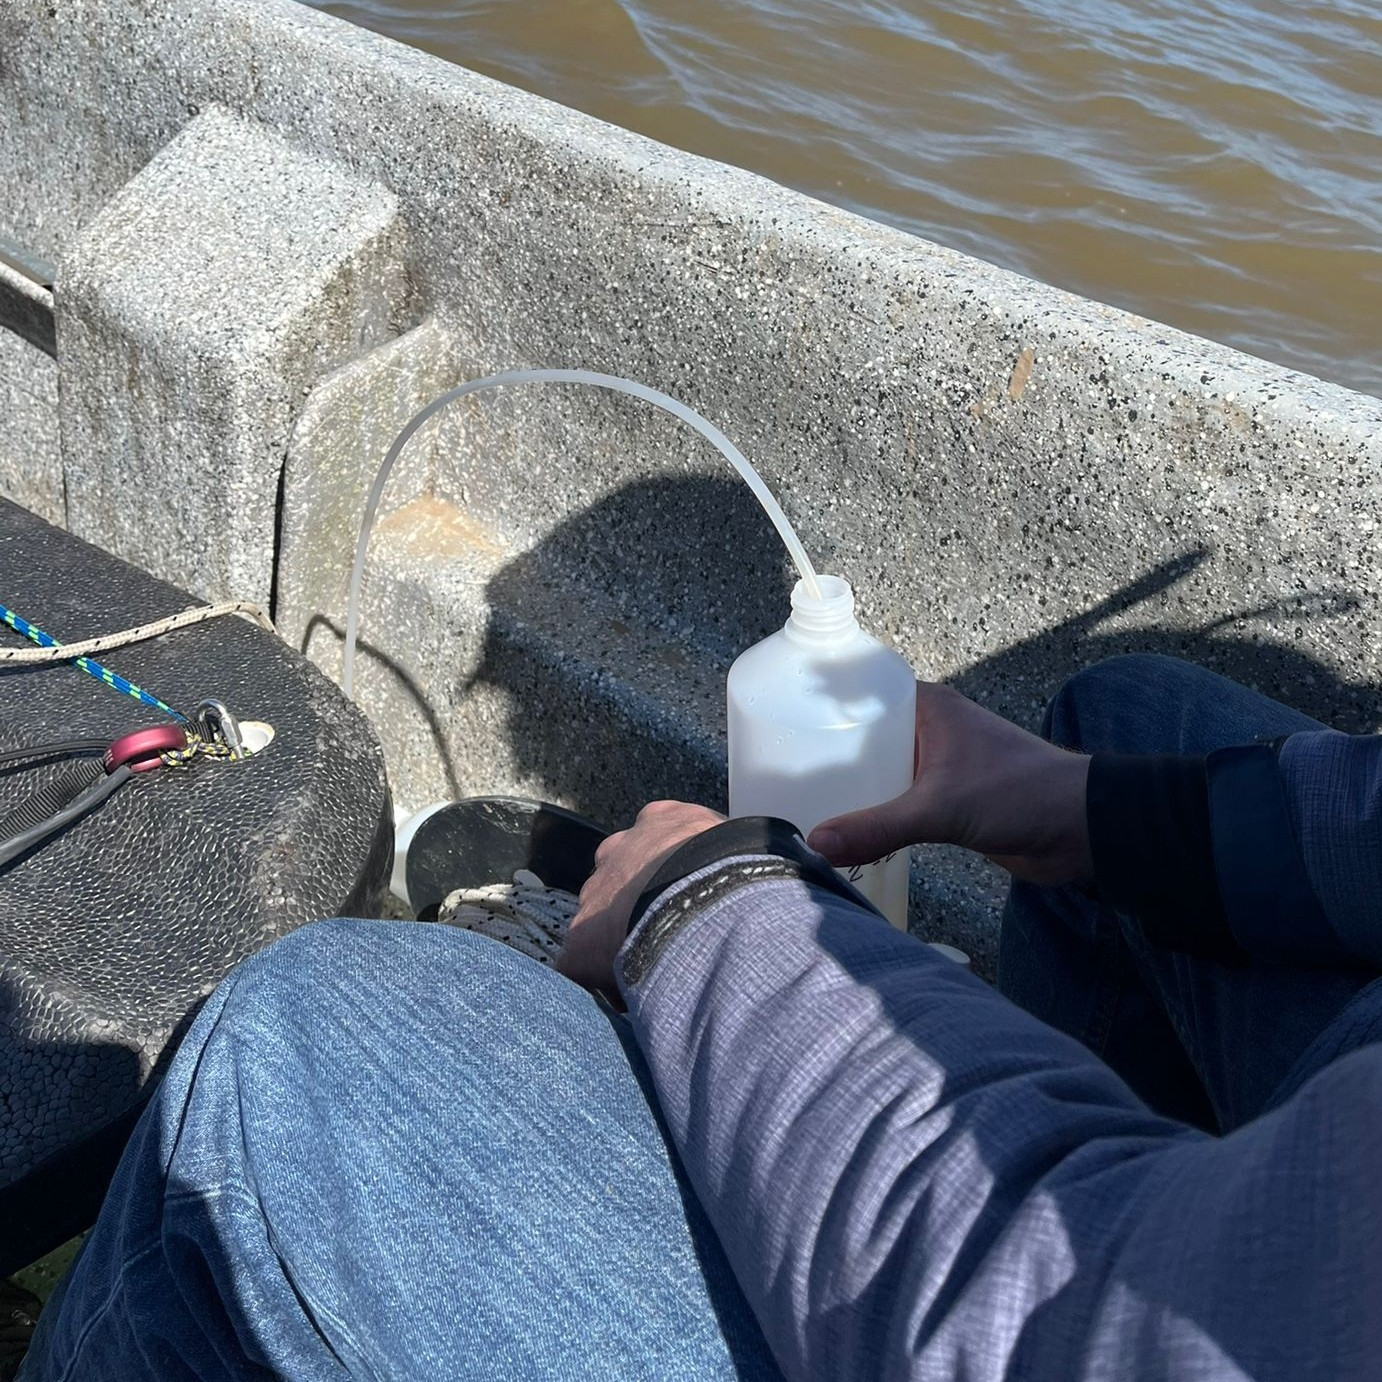
\includegraphics[width=\linewidth]{figures/ch4/fles.jpg}
        \caption{Filling the samples}
    \end{subfigure}
    \hfill
    % Right image
    \begin{subfigure}[t]{0.48\textwidth}
        \centering
        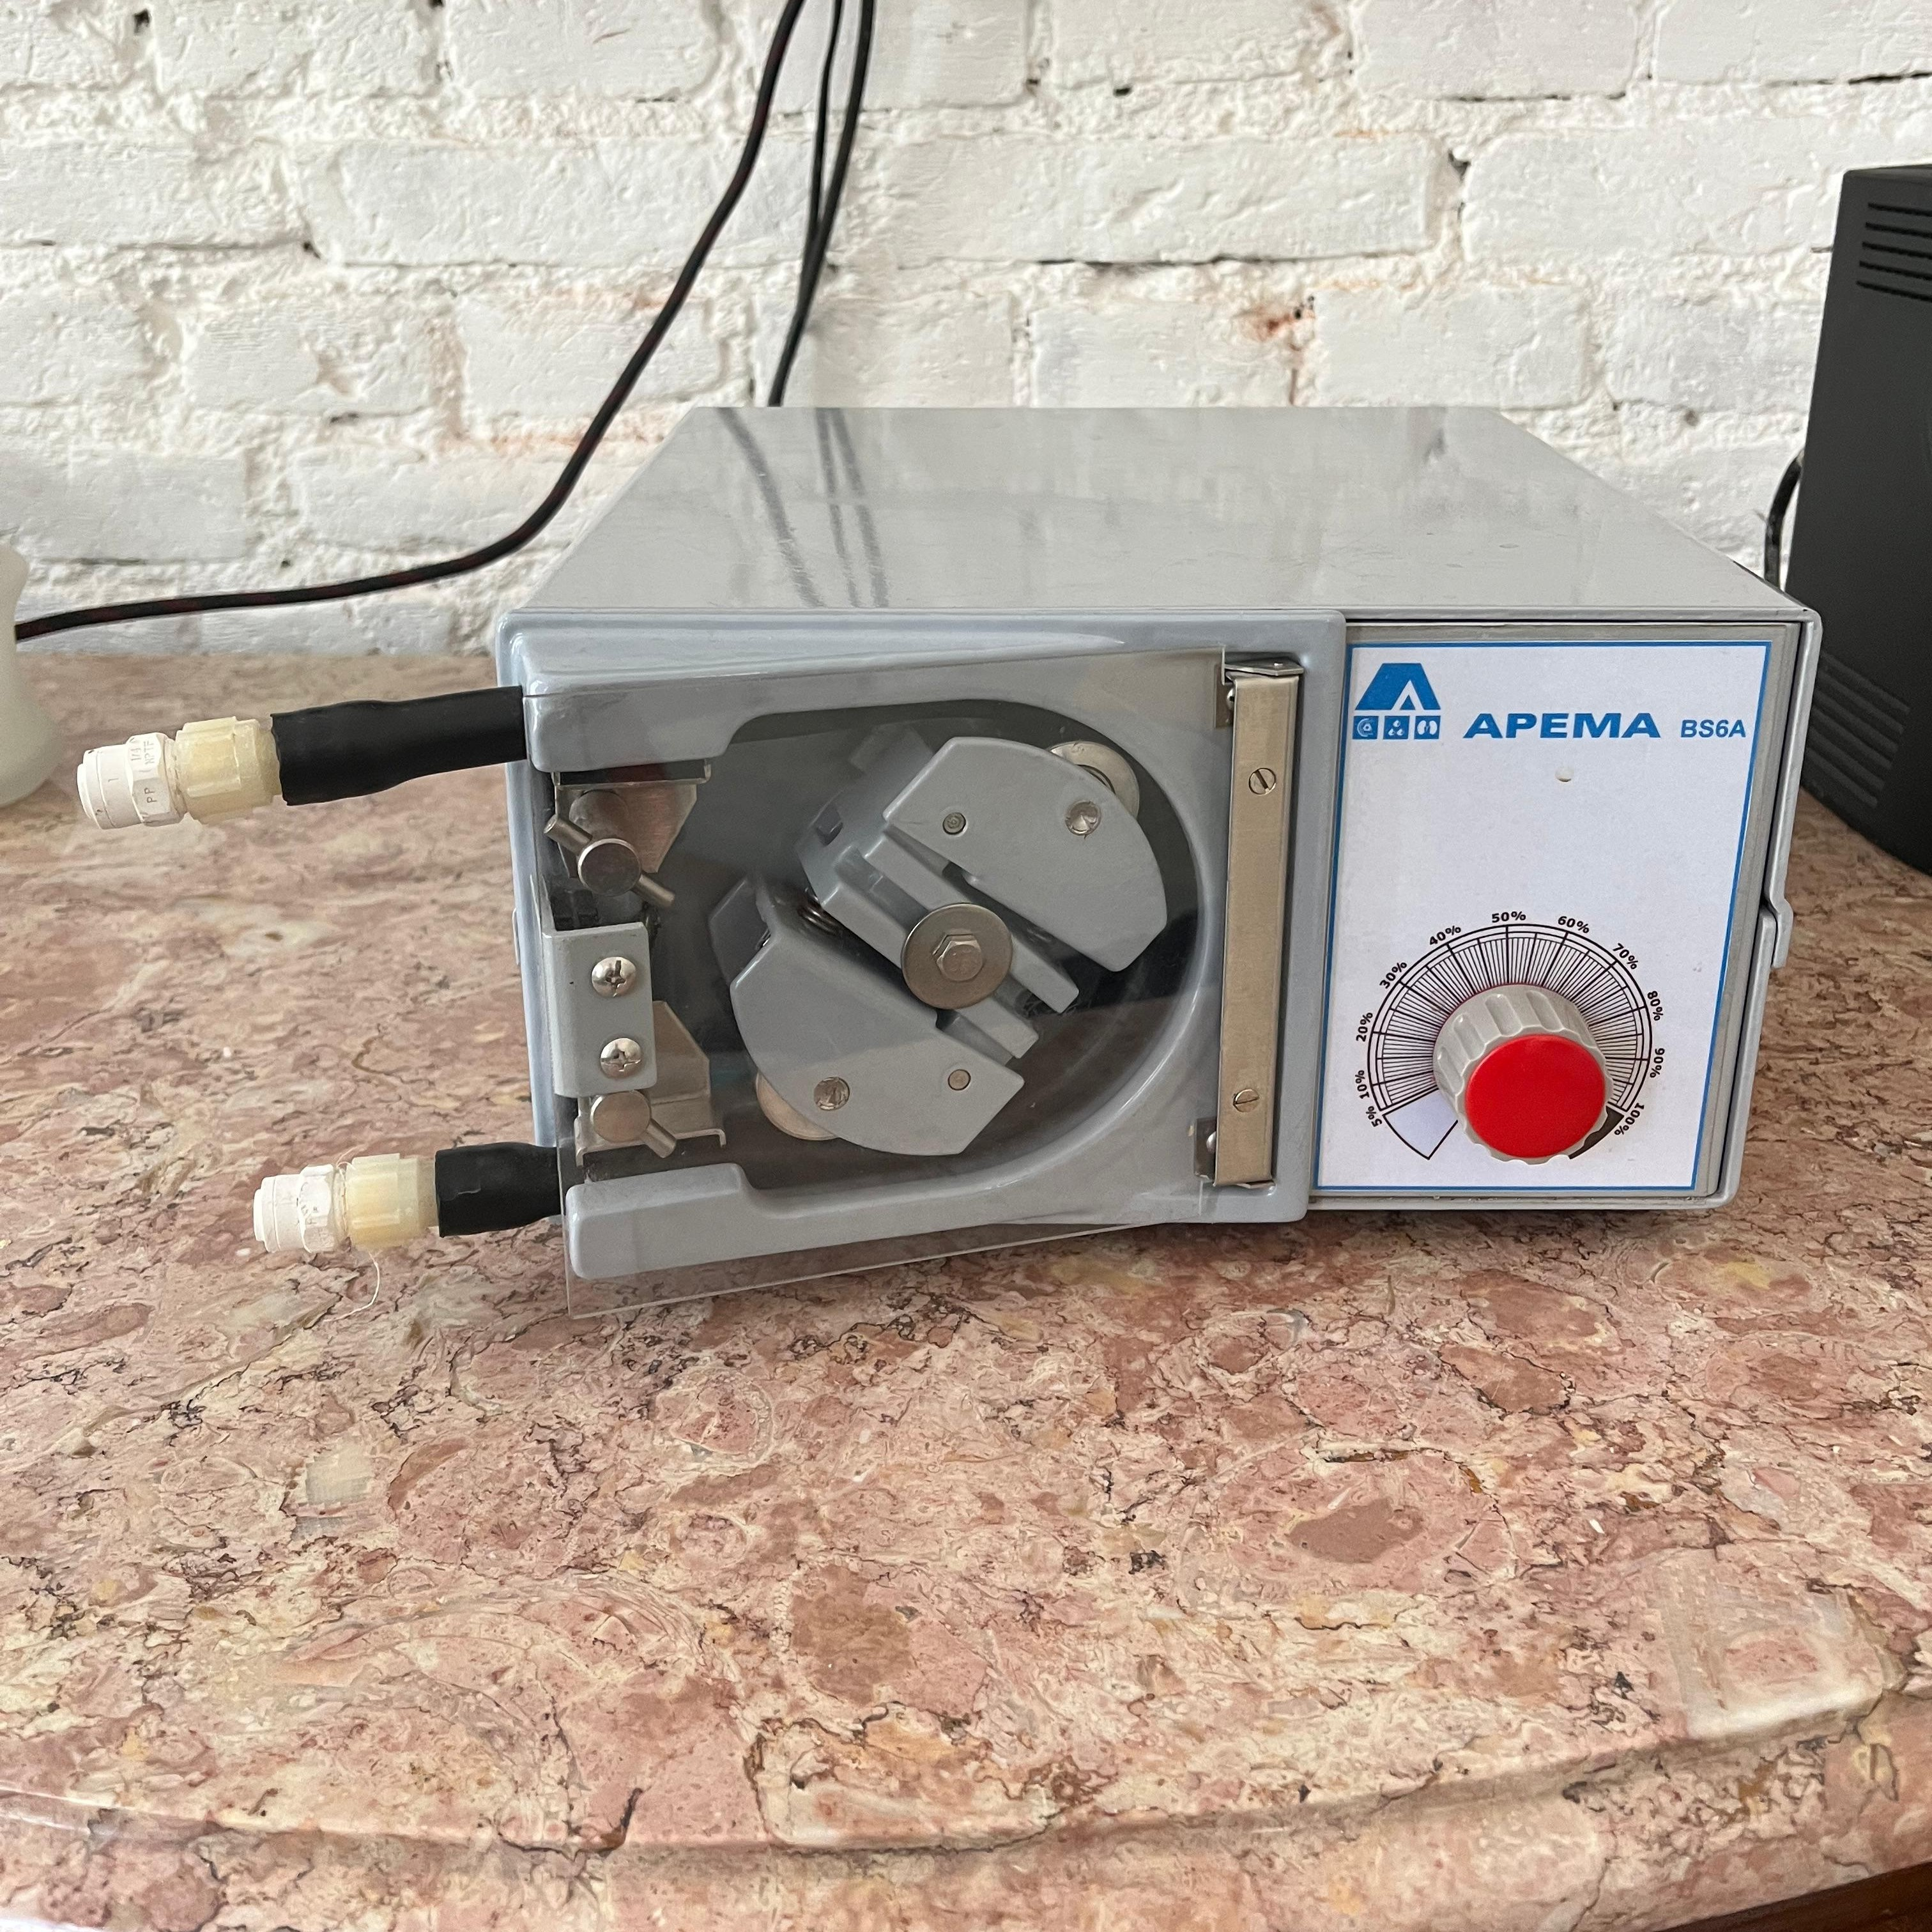
\includegraphics[width=\linewidth]{figures/ch4/APEMA BS6A.jpg}
        \caption{APEMA BS6A device}
    \end{subfigure}
    \caption{Suspended sediment measurements}
    \label{fig:suspended-sediment}
\end{figure}

% In theory, since it was done at different levels of the river, it could potentially indicate a change in concentration from one point upper at Ibicuy to Brazo Largo in the southern, lower part of the study area. From this data, the group could draw even further conclusions.

Finally, the bed load was a necessary measurement for a complete analysis. The method used for this parameter was scraping the bottom layer of the channel with a metal shaped container. The goal was to retrieve samples that represent the granulometry of the bed at different depths. 
During the measurements, a rope was tied to the metal container, which was dropped until it reached the local bed. Then, with help of the current and the movement of the boat, the container was dragged along with the horizontal movement and sediment was gradually collected. Once this was done, the rope and the container were pulled up and restored in the boat. The last step was to collect sediment and put it in a plastic bag. These samples were later analyzed in the lab. The metal container as well as the sediment samples are shown in Figure \ref{fig:bed-load}.

\begin{figure}[H]
    \centering

    % First (large) image
    \begin{subfigure}{0.7\textwidth}
        \centering
        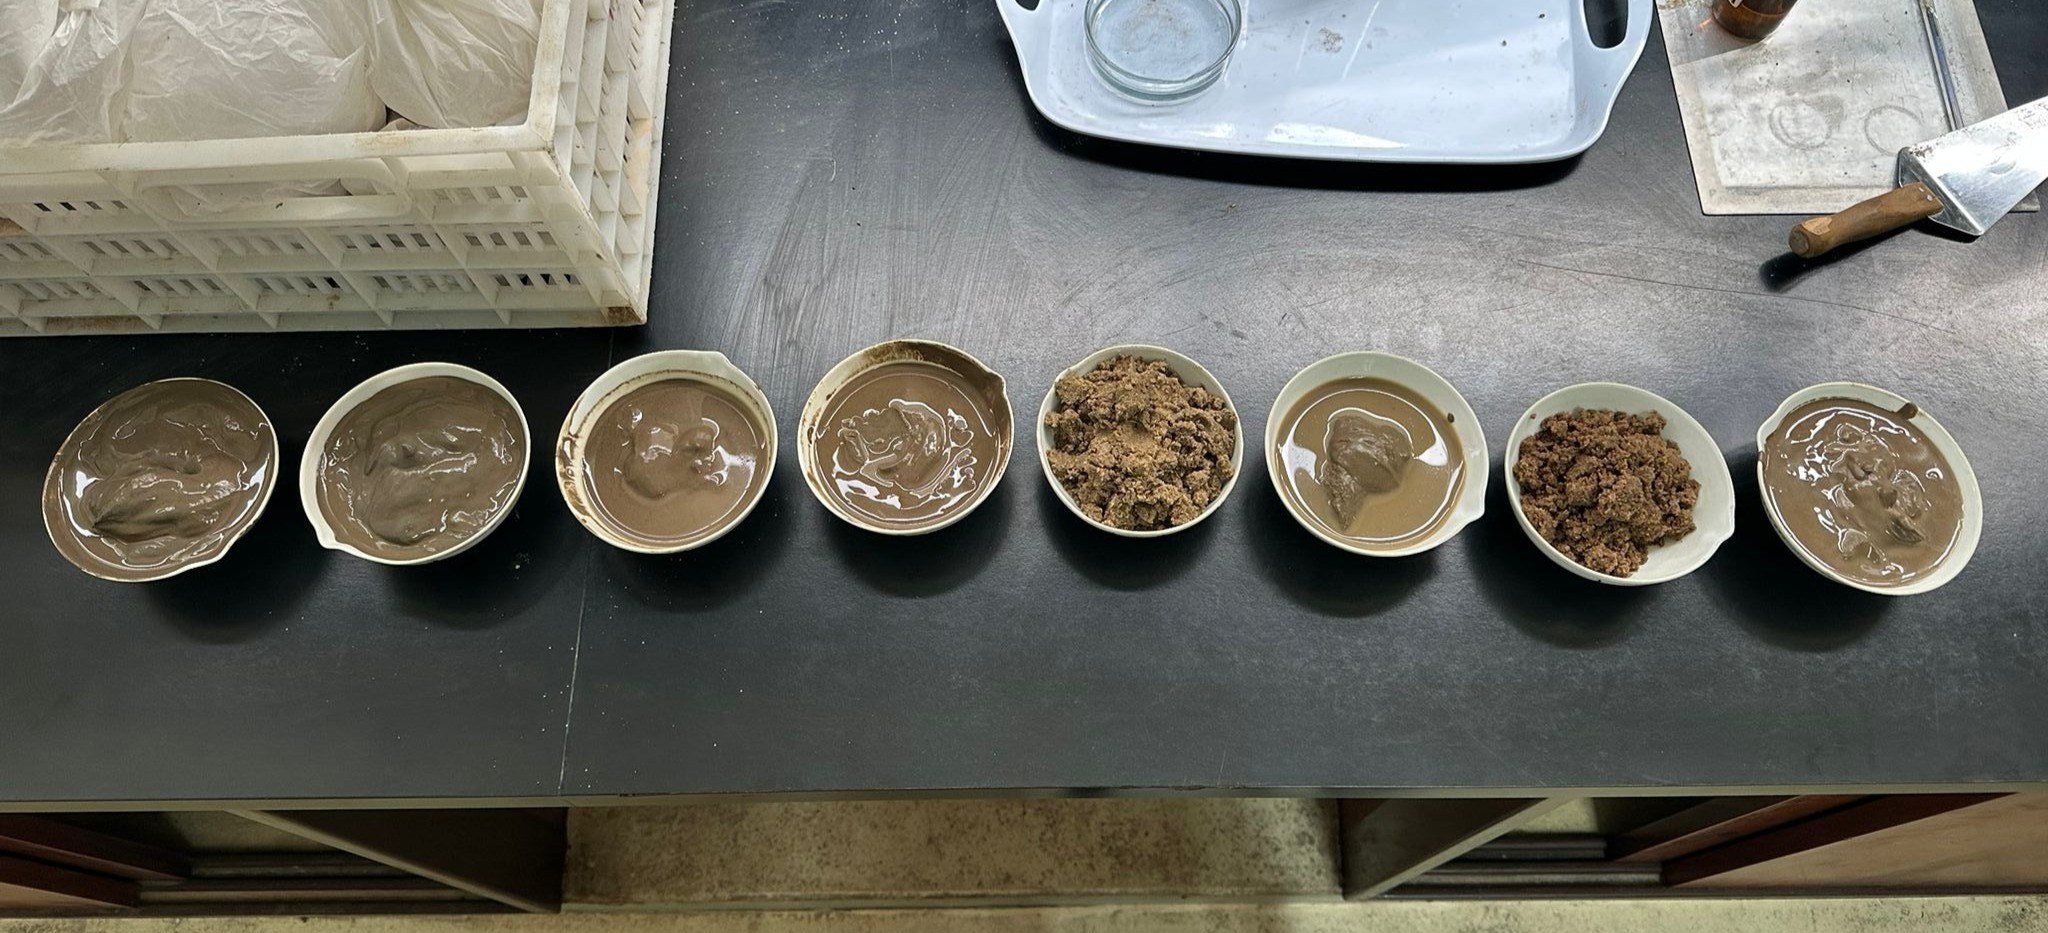
\includegraphics[width=\linewidth]{figures/appendixE/soilsamples.jpg}
        \caption{Bed load samples from the fieldwork}
    \end{subfigure}

    \par\vspace{0.5cm} % use this instead of \vspace alone

    % Two smaller images side by side
    \begin{subfigure}{0.48\textwidth}
        \centering
        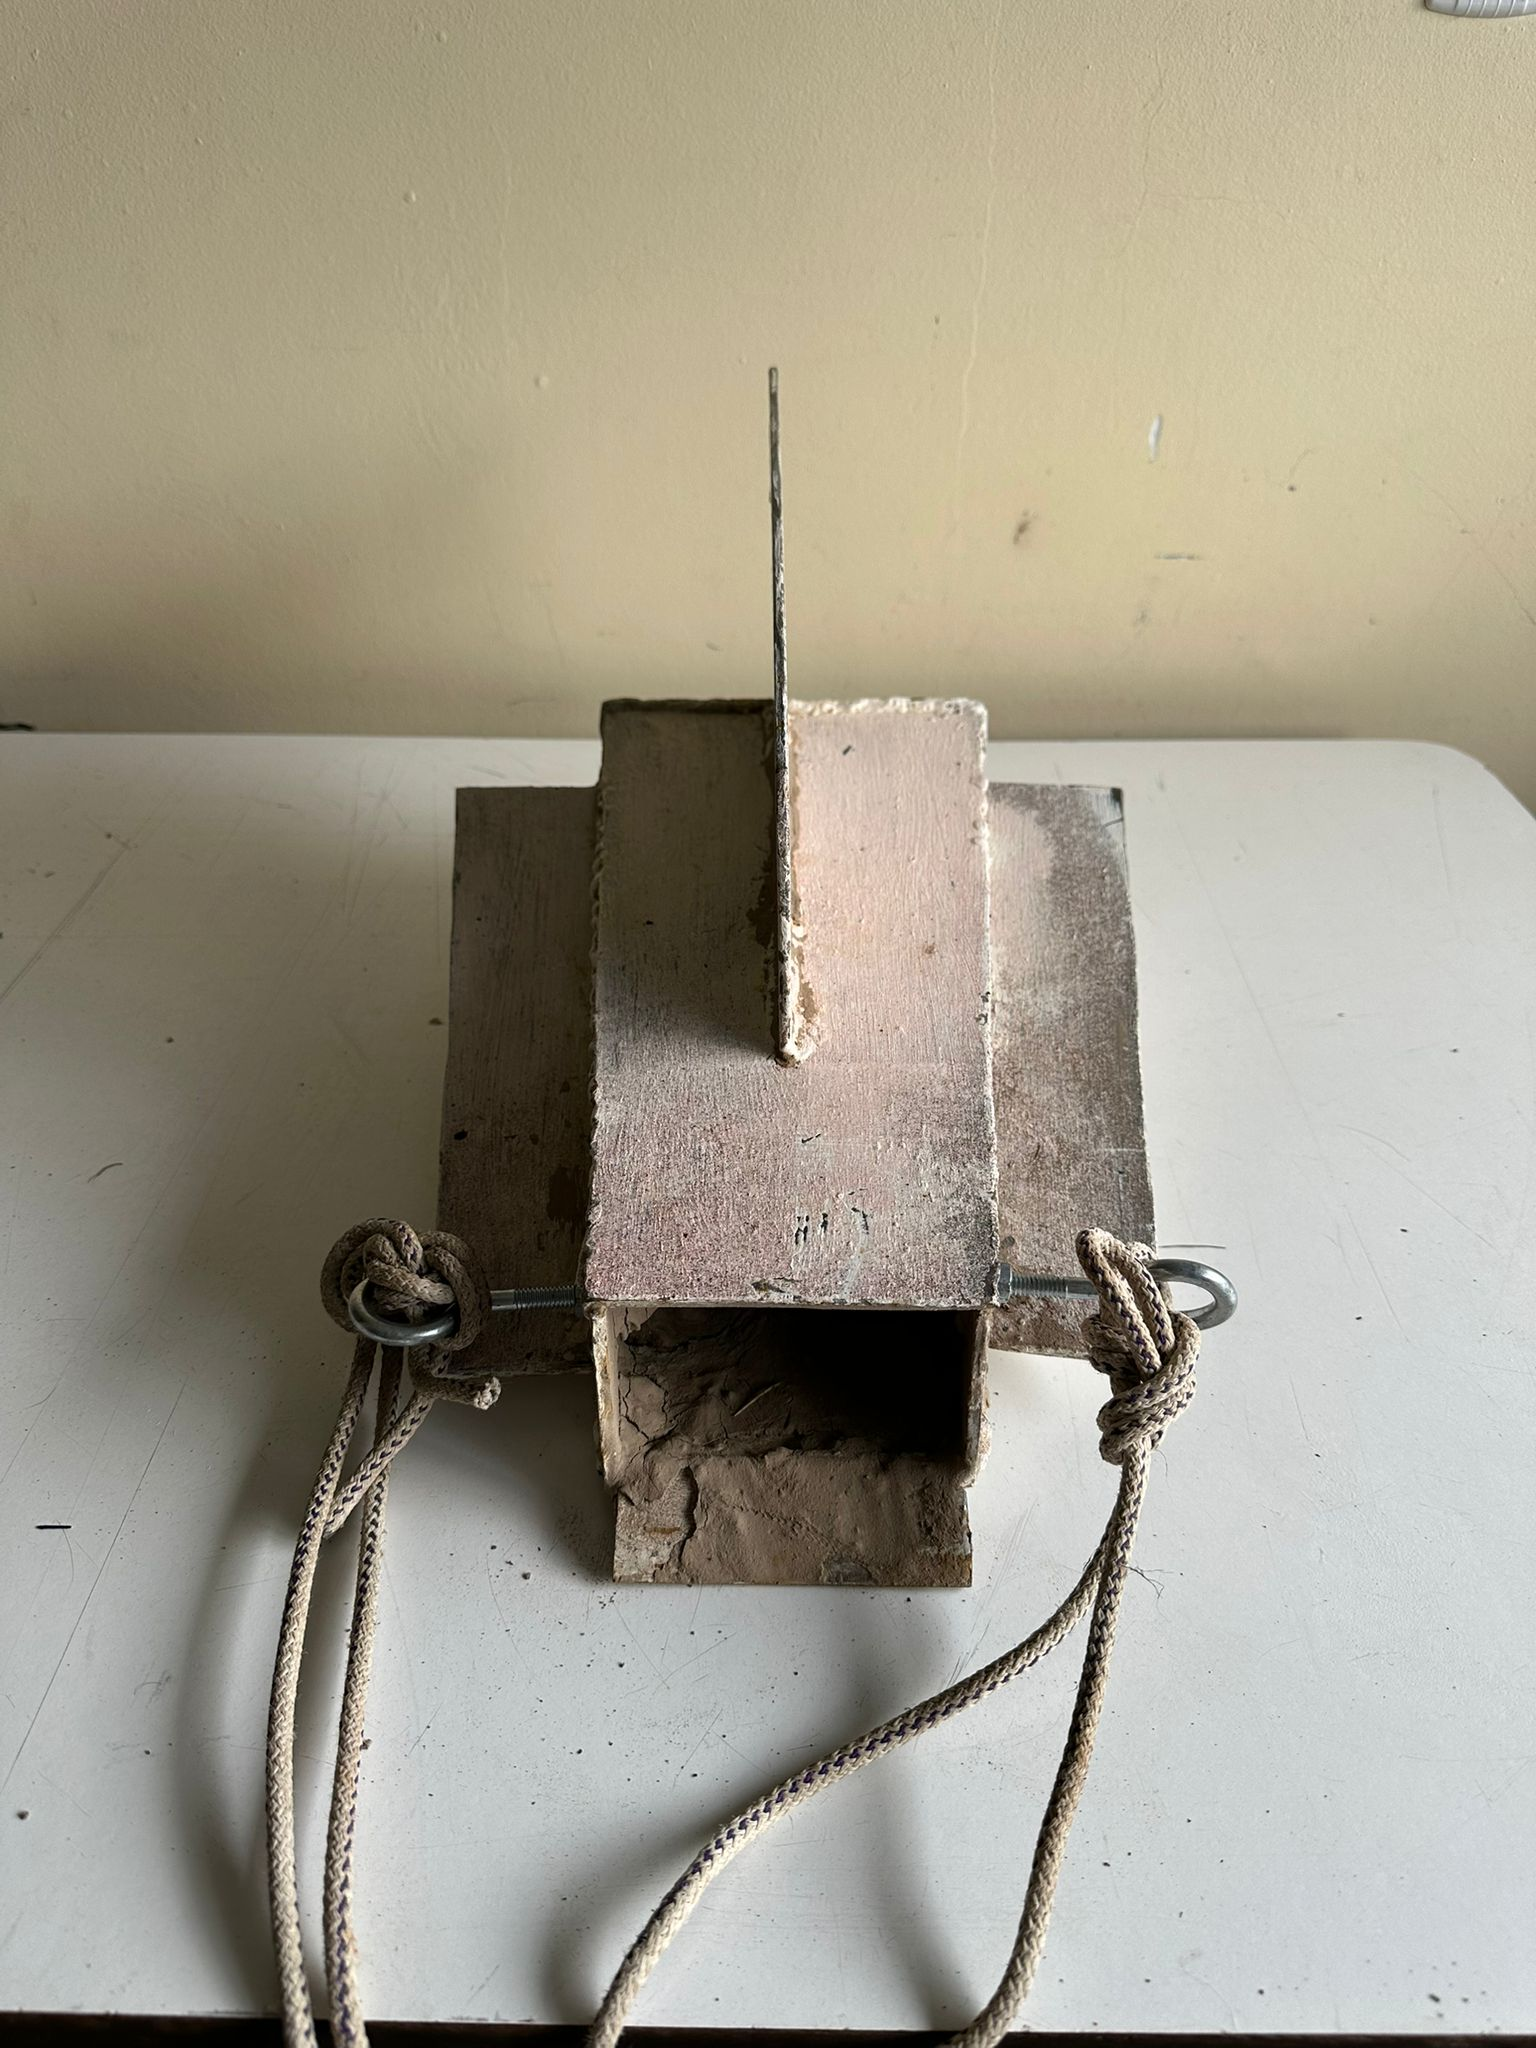
\includegraphics[width=\linewidth]{figures/appendixE/metalcontainer.jpg}
        \caption{Metal container used}
    \end{subfigure}\hfill
    \begin{subfigure}{0.48\textwidth}
        \centering
        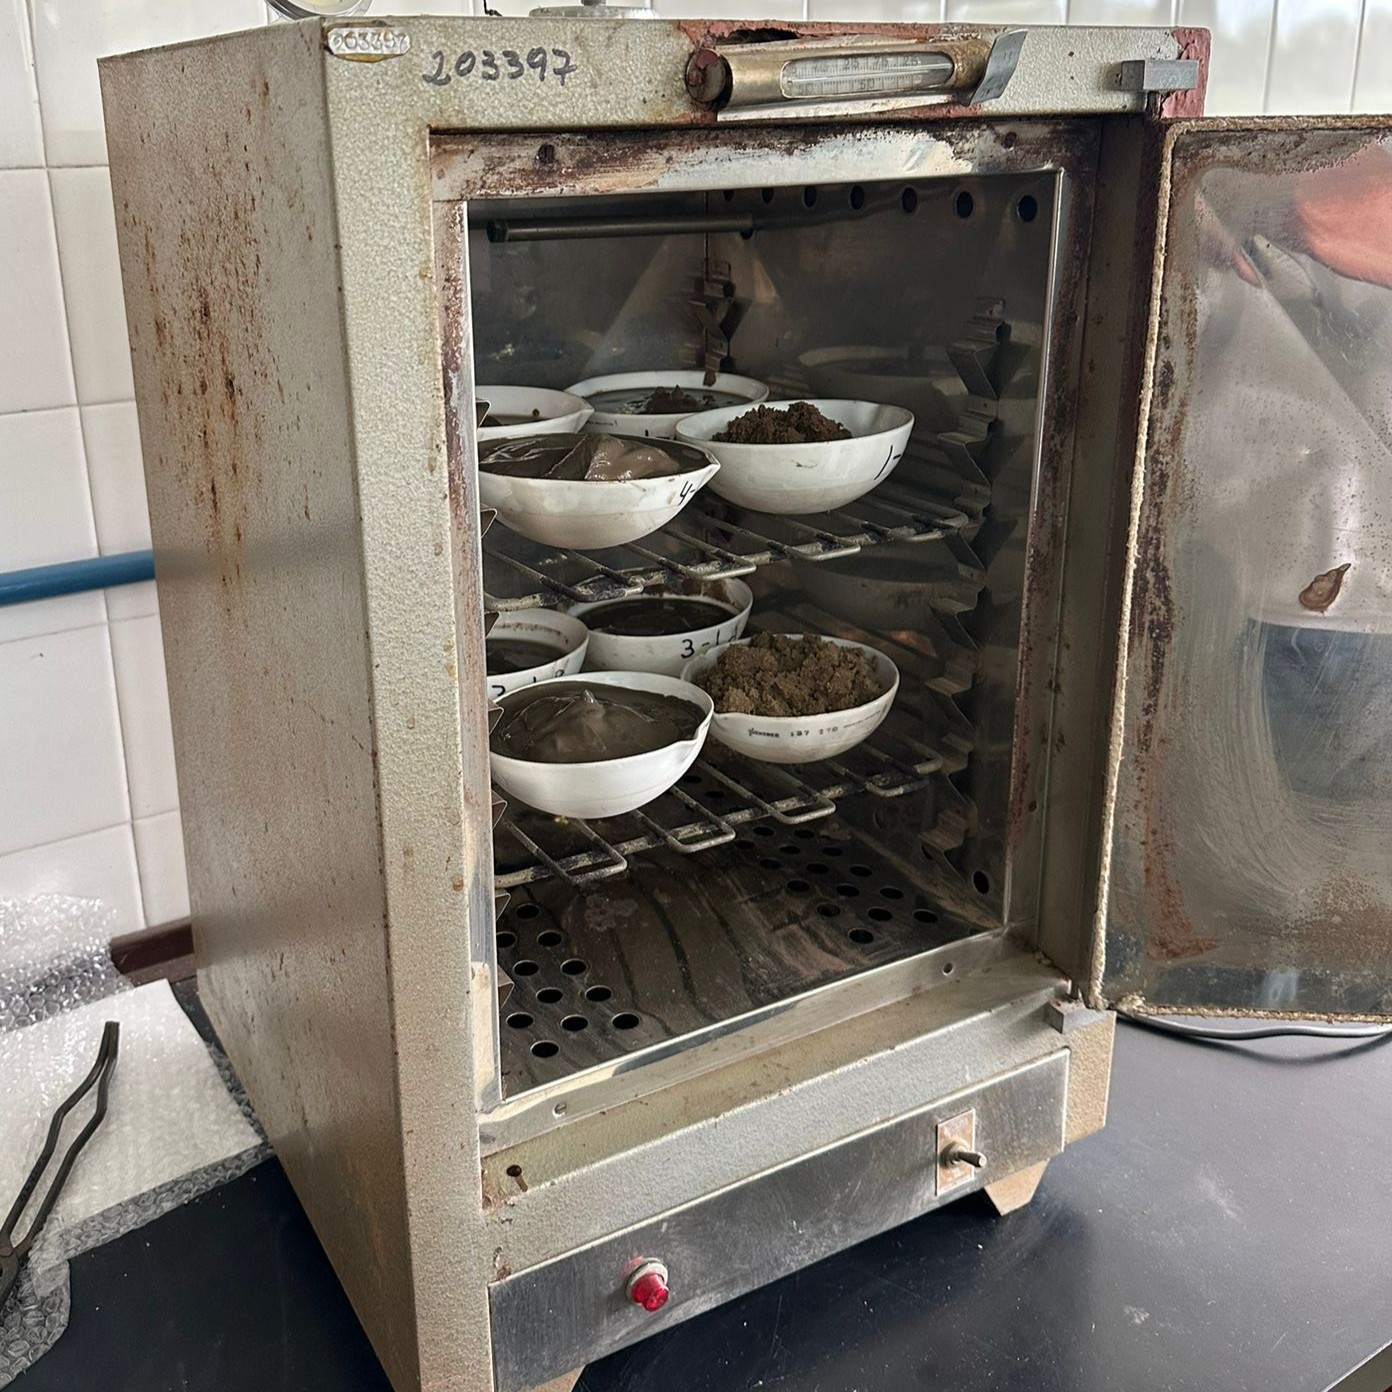
\includegraphics[width=\linewidth]{figures/appendixE/oven.jpg}
        \caption{Oven to dry samples}
    \end{subfigure}

    \caption{Bed load measurements}
    \label{fig:bed-load}
\end{figure}

A total of 7 samples from 4 different locations was collected. The first three locations were the cross sections around the extracting point in the bifurcation of the Paraná Guazú with the Talabera river. For each of these three cross sections, two samples were taken from the soil, one at 10 meters depth and one at 15 meters depth. The final sample was taken at 10 meters depth in the cross section upstream close to Puerto Ibicuy. 

% During the analysis, the soil was dried out to find the components, quality and other parameters of the soil such as porosity which would add up to the results. T

% The bed load samples were all weighed before they were put in the oven. 

All samples were sieved with six differently sized sieves, which took 10 minutes per sample. Before sieving, the samples were crushed to prevent particles from clustering. The sieving machine is presented in Figure \ref{fig:siev} and the whole collection of annotated samples can be found in Appendix \ref{appendix:Lab data}.

\begin{figure}[H]
    \centering
    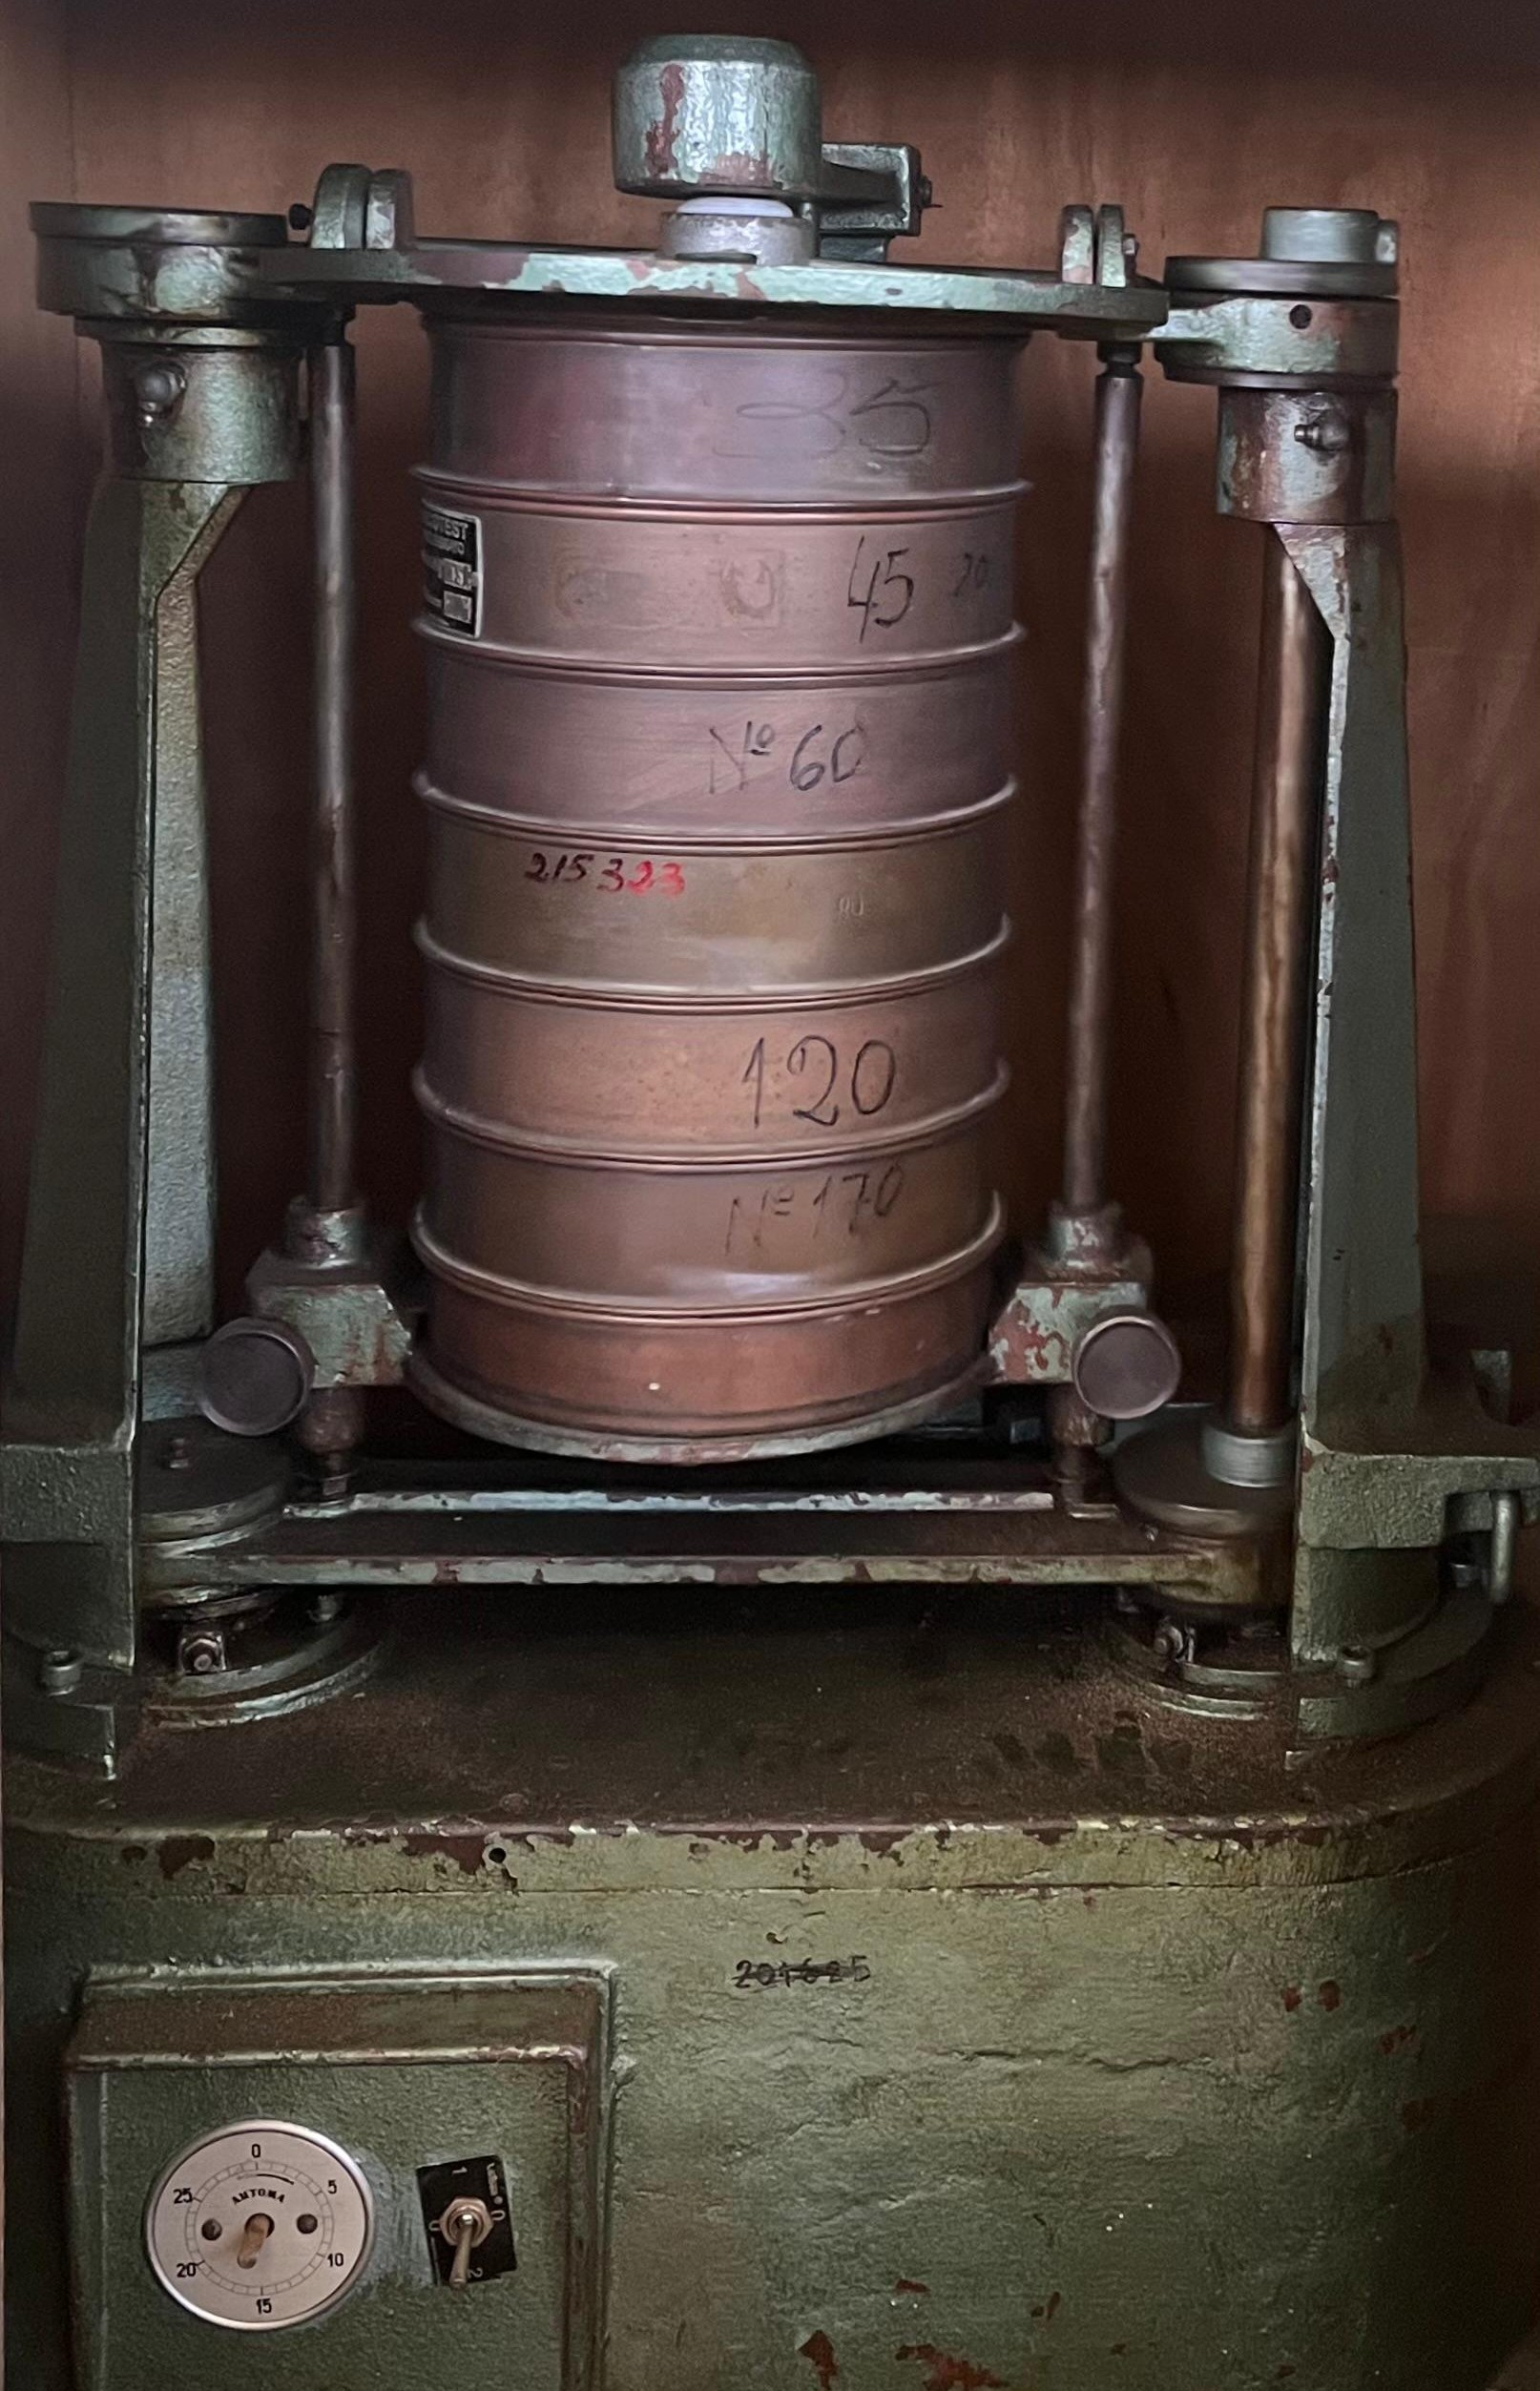
\includegraphics[width=0.35\linewidth]{figures//ch3/siev.jpeg}
    \caption{Sieving machine}
    \label{fig:siev}
\end{figure}

\subsection{Locations of interest}
The measurement campaign was spread out over two main locations. The first location contains a number of cross sections and sediment samples recorded at the confluence of the Talabera and the Paraná Guazú. Figure \ref{fig:measurements day1} shows a summary of the performed measurements. In total, three sections were studied with the following measurements per cross section:
\begin{itemize}
    \item 2 ADCP profiles, yielding bathymetry, discharge and flow velocity;
    \item 2 bed load samples at different locations with different depths;
    \item 5 suspended sediment samples at a single location with varying depths.
\end{itemize}

\begin{figure}[H]
    \centering
    \includegraphics[width=0.75\linewidth]{figures/ch4/day1.png}
    \caption{Measurement location confluence Talabera-Paraná Guazú (\cite{googleearth2025})}
    \label{fig:measurements day1}
\end{figure}

The second location contains measurements at Puerto Ibicuy. Here, cross sections were measured in the vicinity of the confluence of the Ibicuy and the Paraná Guazú. In addition, the echosounder was active. Its recorded tracks can be found in Figure \ref{fig:measurements day2}. The following results were found for location 2:
\begin{itemize}
    \item 6 ADCP profiles: 2 profiles each for the most upstream and most downstream cross section, respectively. 1 profile for those in between; 
    \item 1 bed load sample near Puerto Ibicuy;
    \item 2 longitudinal profiles along the confluence of Talabera and Paraná Guazú (dredging location), measured upstream and downstream to study dune migration. While navigating, GPS applications were used to make sure the paths were identical (see Figure \ref{fig:longprofiles map}).
\end{itemize}

\begin{figure}[H]
    \centering
    \includegraphics[width=0.75\linewidth]{figures/ch4/day2.png}
    \caption{Measurement locations Puerto Ibicuy-Puerto Guazu (\cite{googleearth2025})}
    \label{fig:measurements day2}
\end{figure}

\begin{figure}[H]
    \centering
    \includegraphics[width=0.75\linewidth]{figures/ch3/longprofiles.png}
    \caption{Measurement tracks of longitudinal profiles (\cite{googleearth2025})}
    \label{fig:longprofiles map}
\end{figure}

Bank erosion is a theme of significant importance to this study. During the field trip, critical locations of erosion were visited to understand the stakes at play. These analysis's were often accompanied with pictures taken with a professional drone. The chosen critical location for erosion is the river bank down at the Camping the 'La Blanqueada', situated in the outer side of the curve near Puerto Constanza as seen in Figure \ref{fig:Camping Blanqueada}.

\begin{figure}[H]
    \centering
    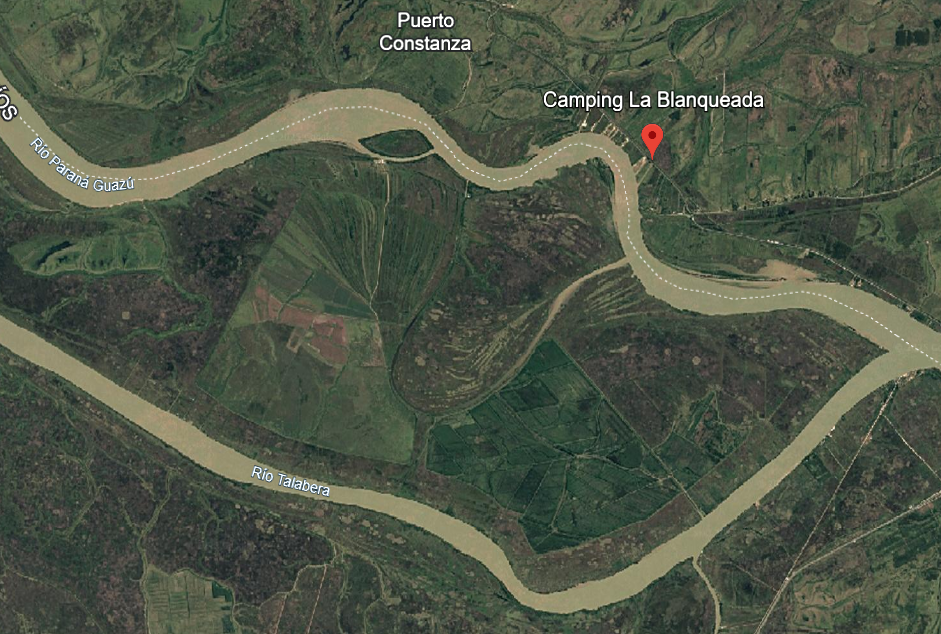
\includegraphics[width=0.75\linewidth]{figures/ch5/Camping Blanqueada.png}
    \caption{Location of camping La Blanqueada (\cite{googleearth2025})}
    \label{fig:Camping Blanqueada}
\end{figure}

This would allow for a comparison with satellite data obtained in the future from software such as Aqua Monitor from Deltares. This software was used to alert critical erosion points along the Paraná Guazú in a broader scale. After the first map data was obtained from the satellite imagery, it was deemed necessary to investigate actual areas and lengths of land that have been subject to water gains and losses. Then the precise location of coast erosion was in turn analysed using Google Earth. The satellite database of Deltares was used for different time stamps, starting from 1984. The reason behind this is that the Deltares Aqua Monitor contains satellite imagery from 1984 until today. The choice was made to analyse the data in time batches of 10 years from 1985 until 2005, then in 5 years from 2005 to 2015, and lastly every 2.5 years in the last decade.

A preview of the maps can be seen in Figure \ref{Aqua Monitor Water Changes 1985-2025}, but the final analysis and conclusions are explained in Chapter \ref{chap:hydroanalysis}. The green parts indicate water losses and the blue parts show water gains over time. For the whole collection of figures, see Appendix \ref{Appendix: Satellite Data}.

\begin{figure}[H]
    \centering
    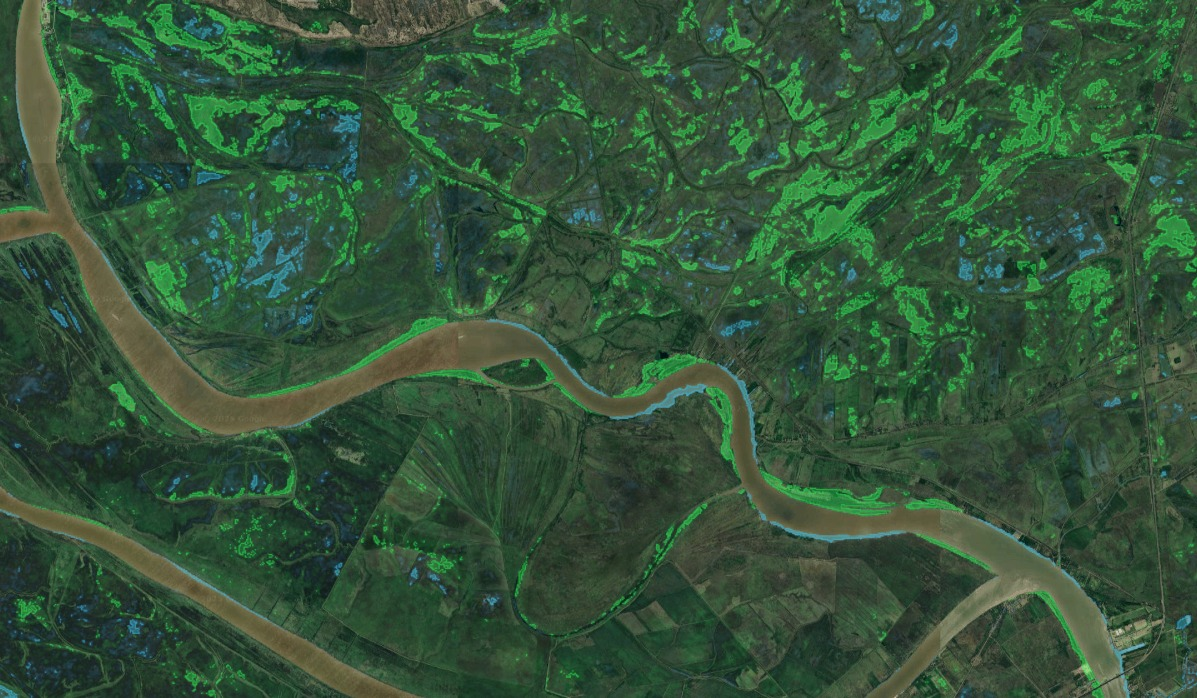
\includegraphics[width=0.75\linewidth]{figures/ch4/1985-2025.jpg}
    \caption{Aqua Monitor water surface changes over the period 1985-2025 (\cite{googleearth2025})}
\end{figure}
\label{Aqua Monitor Water Changes 1985-2025}

\section{Modelling approach}
This section explains the approach that was taken to create the Delft 3D model and the sheet pile model.  

Firstly, ..... .Using the flow velocity one can derive the concentration of the sediment in the study area. This can be done for several locations in order to get an idea of the quantities of sediment that come in through the Rio Ibicuy. Then the last critical point will help us determine the continuation of the concentration of the sediment in the Rio Parana so that any inconsistencies can be linked with the amount of extracted sand in the intersection of the Parana Guazú and Rio Talabera (in the middle of the three critical points on the right hand side of Figure 4.2).

Secondly, a sheet pile model was developed. This resulted in a design that acts as a mitigation strategy against bank erosion. Prior to designing this specific solution, an overview of structural mitigation measures was compiled, and all potential options were evaluated. Subsequently, the design for the selected solution (sheet pile) was created. A flow chart was used to outline the modelling methodology. The flow chart shown in Figure \ref{fig:flow_chart} is divided into three phases. In the first phase, data analysis, literature research was performed to gain a better understanding of the critical locations and parameters necessary for the design. First of all, geological soil conditions including borehole findings were used to assess the different layers and the accompanying soil parameters. Further, hydraulic parameters including bathymetry were provided by INA to assess water level and river bed formation along the banks and finally, structural standards and regulations, the Eurocode, were used to perform structural verifications regarding the ultimate limit and the serviceability limit state.

In the second phase of the model, a sheet pile type was chosen and the gathered data was used to analyse the earth and hydrostatic pressures. Multiple design methods were reviewed, and finally the simplified Padfield and Mair method was chosen to perform the earth and hydraulic pressure analysis. The procedure for calculating the embedding depth of the sheet pile came from the simplified Padfield and Mair method, and the pressure diagrams for the earth and hydrostatic pressure were analysed in Python. By combining the earth and hydrostatic pressures, the balance of moments and the final embedding depth were calculated. Then, the acting components such as shear, bending, and shear buckling were compared to the resistance of the chosen sheet pile profile to access the safety of the design. The final part of phase two consisted of drawing the sheet pile, including unknown design parameters and structural verifications. In the final phase, sustainability aspects for the sheet pile model were considered. More specifically, CO\textsubscript{2} emissions and energy consumption were compared for different materials. This was considered when choosing the material of the sheet pile.

\begin{landscape}
\begin{figure}[H]
    \centering
    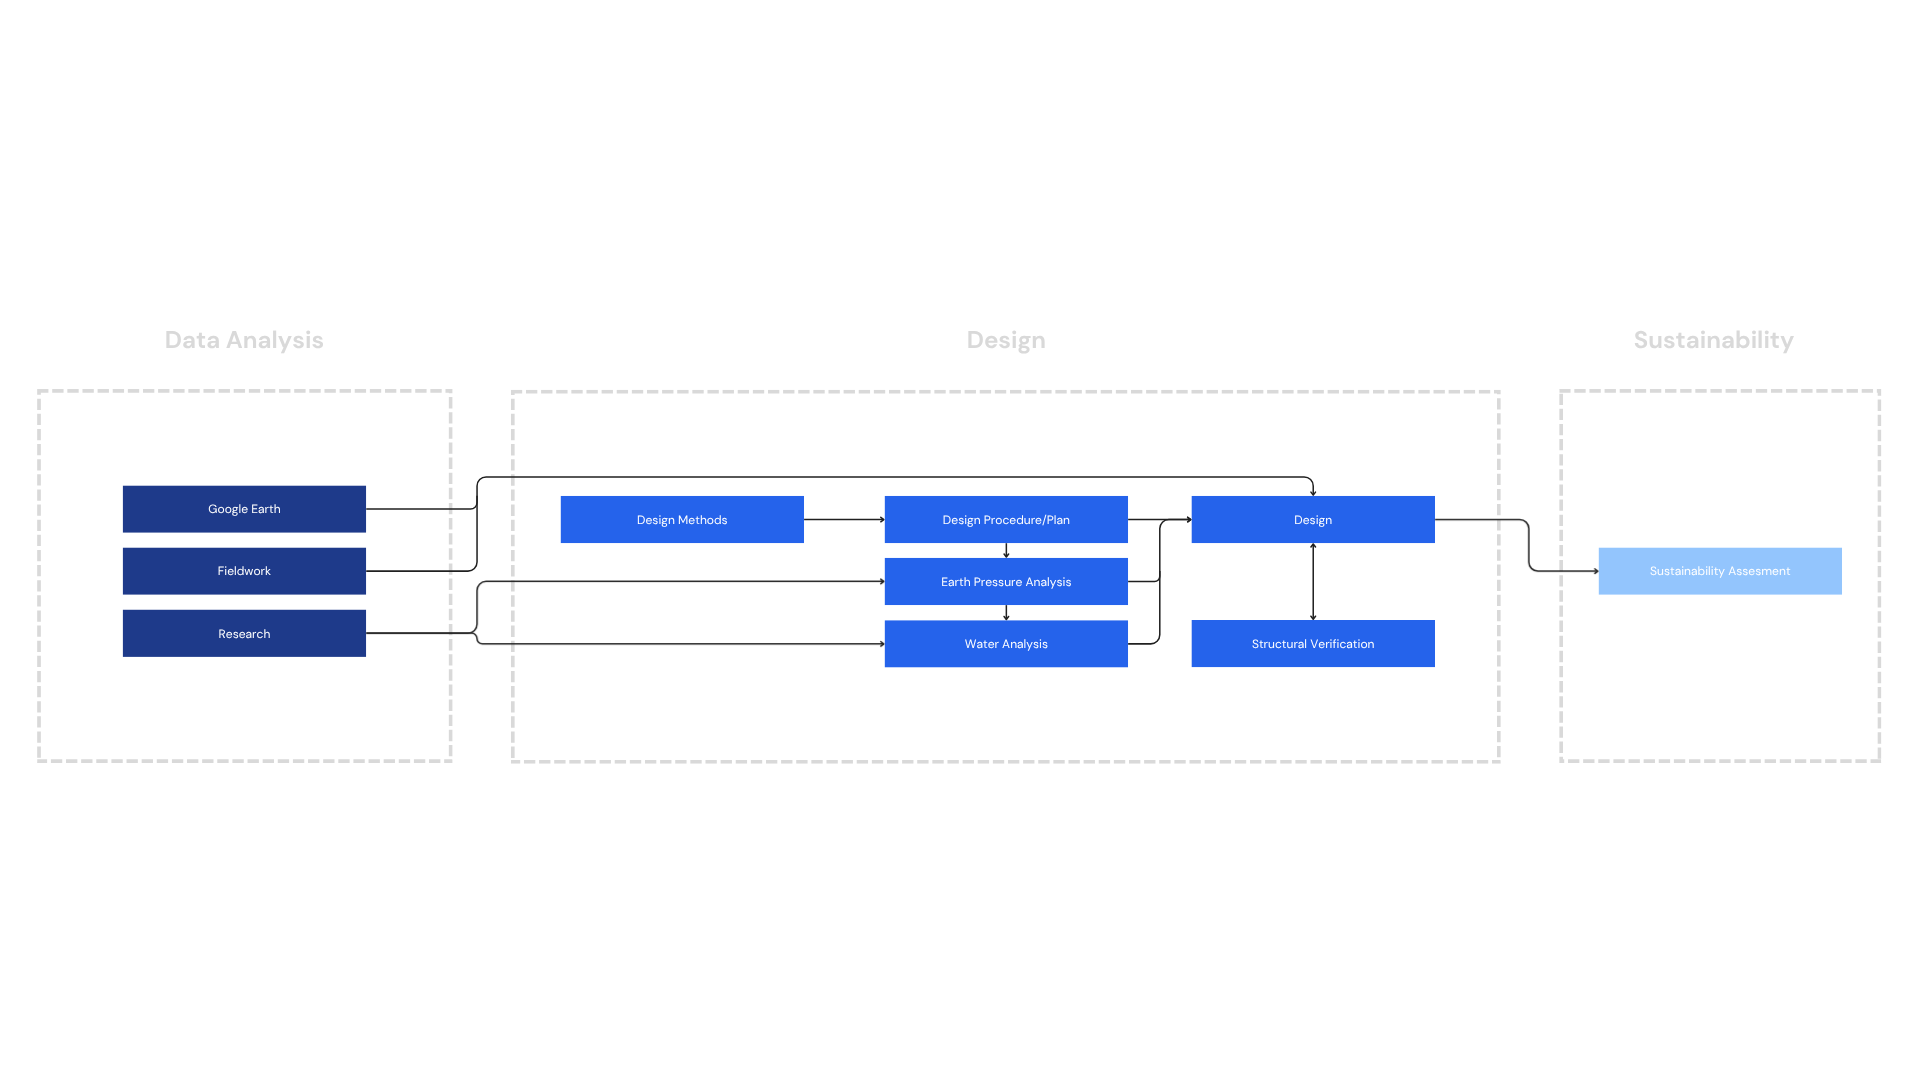
\includegraphics[width=\linewidth]{figures/ch3/FlowChart Structural (3).png}
    \caption{Flow chart sheet pile model}
    \label{fig:flow_chart}
\end{figure}
\end{landscape}
\chapter{Stakeholders}
\label{chapter:stakeholders}
Stakeholders play a crucial role in the study, offering valuable insights and perspectives  necessary to answer the research question. This chapter identifies and analyses the key stakeholders involved, presents the methodology and plan for conducting interviews, and summarizes the main findings from these discussions. Finally, the stakeholder analysis is updated to reflect new information and its implications for the study.


\section{Stakeholder analysis} \label{par:stakeholderanalysis}
This section identifies the relevant stakeholders related to dredging practices in the Rio Paraná Guazú. The interests and goals of these stakeholders are explained, and a power versus interest matrix is used to illustrate their relevance to the project.

\subsection{Stakeholders description, interest, and power}
All relevant stakeholders are identified for this project based on personal investigations and suggestions by INA staff. The complete overview is listed in Table \ref{tab:stakeholders} and will be discussed in the following sections. Investigation of the relevant parties lead to a list of 8 stakeholders. The stakeholder descriptions are given in Table \ref{tab:stakeholders-description}, and their interests and goals given in Table \ref{tab:stakeholders-interests-goals}. All stakeholders were contacted to arrange interviews.

\begin{table}[H]
\centering
\caption{Potential stakeholders and their roles}
\begin{tabularx}{\linewidth}{p{3.5cm}X} % narrower first column
\toprule
Stakeholders & Role \\
\midrule
Dredgers & Extraction of sand and gravel from shallow river areas. \\
Prefectura Naval Argentina (PNA) & Protection of rivers and maritime territory, and functions as coast guard and river police. \\
Agencia Nacional de Puertos y Navegación (ANPYN) & Oversight of signalling systems, dredging operations, and maintenance of the Main Waterway. \\
Ports & Handling, storing, and trading of goods and dredged material. \\
Fishers & Artisanal and independent fishing activities for local and regional markets. \\
NGOs & Non-profit organizations advocating for environmental protection and community interests. \\
Landowners & Owners of riverfront or adjacent lands, may lease property for port or dredging operations. \\
Filmmakers & Filmmakers documenting trade and social impacts of the Paraná–Paraguay waterway. \\
\bottomrule
\end{tabularx}

\label{tab:stakeholders}
\end{table}



\begin{table}[H]
\caption{Stakeholder descriptions}
\centering
\begin{tabularx}{\linewidth}{p{3.5cm}X} % fixed width first column
\toprule
Stakeholders & Description \\
\midrule
Dredgers & Dredgers extract sand and gravel from the Paraná Guazú, ranging from small independent vessels to organized groups of boats (areneros) and larger hopper ships. They operate mainly in shallow areas where simple extraction methods are possible, transporting the material to nearby ports such as Ibicuy or Brazo Largo. \\
\midrule
Prefectura Naval Argentina (PNA) & Prefectura Naval Argentina (PNA) serves as Argentina’s coast guard and river police, operating under the Ministry of National Security. It is responsible for protecting rivers and maritime territory, ensuring safety, security, and regulatory compliance. In the Paraná Guazú, PNA plays a key role in monitoring dredging activity and maintaining lawful use of waterways. \\
\midrule
Agencia Nacional de Puertos y Navegación (ANPYN) & Agencia Nacional de Puertos y Navegación is the authority in charge of implementing and controlling the signalling system, as well as overseeing dredging and maintenance along the Main Waterway, which includes the Paraná Guazú. As an independent agency within the Ministry of Economics, it ensures navigational safety and operational continuity of ports and waterways. \\
\midrule
Ports & Ports serve as key logistical hubs for handling and storing goods extracted or transported along the Paraná Guazú. They provide the facilities where dredged sand is unloaded and traded, connecting local extraction activities with broader commercial markets. Their role is essential in enabling the flow of materials and supporting both regional trade and industrial supply chains. \\
\midrule
Fishers & Fishers on the Paraná Guazú depend on the river’s abundant fish resources, particularly migratory species such as sábalo, surubí, boga, pacú, and dorado. Most are independent artisanal fishers, selling their catch through middlemen, freezing plants, or informal markets. Although associations exist in the region, they hold little influence in decision-making over river use and management. \\
\midrule
NGOs & Non-governmental organizations play a role in monitoring the social and environmental impacts of activities along the Paraná Guazú. They advocate for sustainable river management, community interests, and the protection of ecosystems affected by dredging and trade. Their involvement adds external oversight and pressure on both companies and authorities to adopt responsible practices. \\
\midrule
Landowners & The landowners in the area have an interest in the sand mining activities. After all, some of them live in the area and experience negative consequences to their land. Jorge Moriatan is a local landowner that was contacted during the study to tell about his experiences related to dredging. \\
\midrule
Filmmakers & Alejo Di Risio is a filmmaker who directed a documentary on the Paraná–Paraguay waterway, focusing on the impacts of trade along the river system. His work highlights the economic and social dimensions of waterway use, bringing public attention to stakeholders and their activities. He was also contacted during this study to provide additional insights into stakeholders and businesses connected to the waterway. \\
\bottomrule
\end{tabularx}
\label{tab:stakeholders-description}
\end{table}

From the interviews that were carried out, the stakeholder's interests and goals were derived. In Appendix \ref{chap:interviews}, the fully typed out interviews can be found and the summarized results are given in Section \ref{sect:interviewresults}.

\begin{table}[H]
\centering
\caption{Stakeholders interest and goal}
\begin{tabularx}{\linewidth}{p{3.5cm}XX}
\toprule
Stakeholders & Interest & Goal \\
\midrule
Dredgers & Access to shallow river areas for sand extraction. & Sell extracted sand to nearby ports and local markets for income. \\
\midrule
Prefectura Naval Argentina (PNA) & Safety and security of rivers and maritime territory. & Enforce regulations, monitor dredging, and ensure lawful use of waterways. \\
\midrule
Agencia Nacional de Puertos y Navegación (ANPYN) & Oversight of navigation safety and waterway infrastructure. & Implement signalling systems, maintain dredging operations, and secure efficient transport. \\
\midrule
Ports & Handling and trading of goods and dredged material. & Strengthen logistical capacity and support regional trade flows. \\
\midrule
Fishers & Access to fish resources in the Paraná Guazú. & Sustain livelihoods through artisanal fishing and market sales. \\
\midrule
NGOs & Environmental protection and community rights. & Promote sustainable river management and hold stakeholders accountable. \\
\midrule
Landowners & Protection of riverfront property and prevention of erosion, flooding, or land loss. & Safeguard land rights and preserve long-term property value. \\
\midrule
Filmmakers & Research and documentation of waterway dynamics. & Raise awareness through film on trade, impacts, and stakeholder activities. \\
\bottomrule
\end{tabularx}

\label{tab:stakeholders-interests-goals}
\end{table}

\subsection{Stakeholder's influence}
After identifying stakeholders, it is important to evaluate their power and interest in the project. This is visualized using a power versus interest matrix, with power on the vertical axis and interest on the horizontal axis. Analysing this matrix informs strategies to approach specific stakeholders. In addition to interest and power, a support-opposition matrix is analysed to visualize the likelihood that a certain stakeholder will support or oppose the project.

The power versus interest matrix is divided into four parts, illustrated in Figure \ref{fig:power-interest}. The quadrants represent the power and interest that a particular stakeholder has in terms of low or high. High power and high interest are referred to as the key players, and these will be of most importance to the project. Next, the quadrant with low power and high interest is considered the subject. Those with high power but low interest are determined as the context setters. The context setters are not closely related to the project, but can be of great importance. The quadrant of low power and low interest is recognized as the crowd.

\begin{figure}[H]
    \centering
    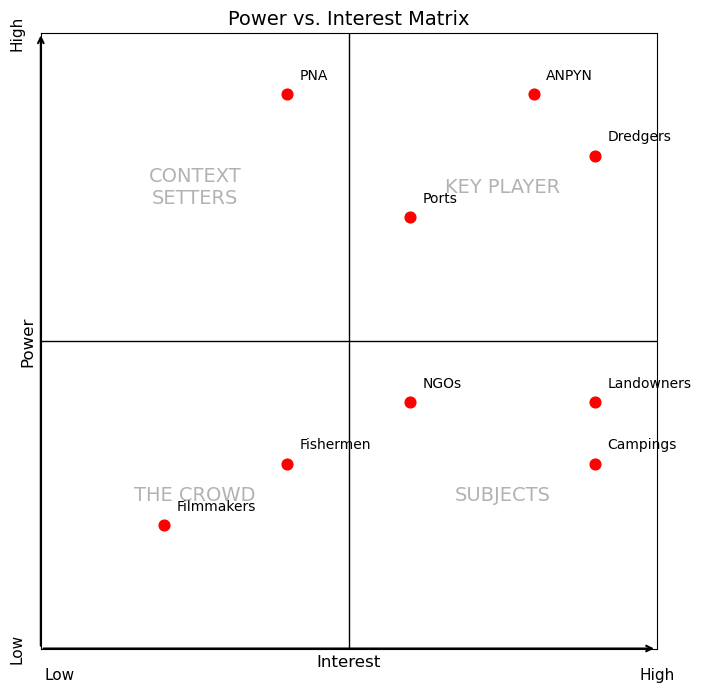
\includegraphics[width=0.65\linewidth]{figures/ch3/PowerVSInterest.png}
    \caption{Power vs. Interest}
    \label{fig:power-interest}
\end{figure}

The key players, stakeholders with both high interest and power, are of great importance to the project. Among this group are actors with a great economic interest in the dredging activity: the dredgers and the ports. They are commercially organized, which is why their power is also high. Finally, the ANPYN, being the responsible government agency, is an actor of great interest and power. This is the most important group for project success. These stakeholders must be actively engaged and managed through continuous and tailored communication. They should be consulted in decision-making and kept up to date on risks, challenges, and progress. Building strong relationships with them is vital to ensure their ongoing support and alignment with project goals.

Context setters have high power but relatively low interest in the project. Within this group, the PNA can be found. Being a major government organization responsible for safety and compliance with maritime laws, they have significant authority and influence. However, their focus is mainly on guarding the safety on the water, more than supervision of the dredging activities. The context setters are of moderate priority to the project. Since they hold power, it is important to prevent dissatisfaction that could derail progress. The dealing strategy should focus on maintaining their satisfaction without overwhelming them with details. Periodic check-ins and concise reports or briefings can help with this. This ensures they feel respected and considered, as their influence may become critical if project circumstances shift.

On the bottom right of the graph, one can find the subjects, a group that holds high interest in the project but has less power. Here the NGOs, landowners and campings can be found. Because of ideological beliefs or personal concerns, their interest in the project is high. However, due to a limited degree of organization their power is not substantial. This is another group of moderate priority to the project. The stakeholders care deeply about the project but lack significant power to influence its direction. Any enthusiasm from this group can be valuable and should thus be maintained and leveraged if useful. However, it is perhaps more likely for stakeholders in the group of subjects to be opposed to the project. In this case, their high level of interest may manifest as opposition or criticism. Therefore, it is important to actively listen to their concerns and provide information to address any misconceptions or fears. This way, any opposition can be managed and maintained.

Finally, there is the crowd. Stakeholders in this group are characterized by a low power and low interest in the project. The journalists and fishers fall under this group: they are largely unorganized and, although sometimes important, sand mining is not their main concern. This group is the least important to the project's outcomes. Since their involvement is not crucial, one should avoid overloading them with unnecessary details and should instead only monitor them. It is possible to update the crowd on important progress as to prevent disengagement or frustration.

The support-opposition matrix is divided into four parts and a linear trend line is based on the points given to the stakeholders. On the vertical axis, the division between support and opposition is made, while on the horizontal axis, the power is represented. For the degree of power, the power versus interest matrix, in Figure \ref{fig:power-interest} was used. The stakeholders support or opposition for the project was based on the interviews held during the field trip and is shown in Figure \ref{fig:support-opposition-power}.

\begin{figure}[H]
    \centering
    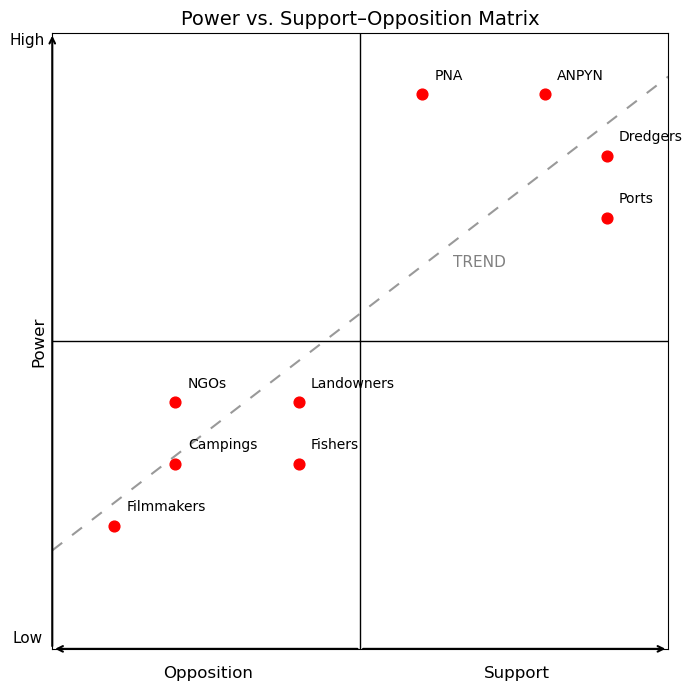
\includegraphics[width=0.65\linewidth]{figures/ch3/Support-OppositionVSPower.png}
    \caption{Power vs. Support-Opposition}
    \label{fig:support-opposition-power}
\end{figure}

With multiple stakeholders who have different interests and goals, it is of importance to know the competing interests. Among the various stakeholder interests, the focus will be on the competing economic and environmental interests. The first competing interest is the economic growth of the area versus environmental protection. The dredging activities of the Paraná Guazú and Ibicuy stimulate the economic growth of the area and are one of the income streams for the dredgers and ports. These economic benefits are prioritized over the environmental protection of the river and the river banks. Environmental protection is of interest to fishermen and NGOs operating on the Parana waterway. Their goal is to minimize the environmental impact of dredging. This leads to a competing interest, as dredging will have effects that come at the expense of the environment.

A second competing interest is  safety and regulations versus  profits made by dredging activities. For business-related stakeholders, the interest in making profits is of greater value than the safety regulations created by the governmental organizations. The PNA and ANPYN regulate the safety of waterways, which can impose restrictions on the amount of sand a dredger can extract or the frequency limit for dredging activities. This can be a concern, as the regulations will cut profits of ports and dredgers, which lie between the strict enforcement and the loosely regulated operations of dredgers.

Another area of conflicting interests can be summarized by local livelihood versus local development. The dredging of the river will lead to income for the ports and dredgers, which, through taxes, can attribute to development of the region. This can be of interest to local businesses and communities. On the other hand, there is the local livelihood that may be of even greater importance to the community. As mentioned before in chapter \ref{chapter:background}, dredging can reduce water quality, fish spawning and land loss, among other things. A reduction of fish in the river will harm food security in the region and is even more problematic for the fishers, since this directly hurts their businesses and livelihood. Likewise, land loss through increased erosion negatively affects landowners, reducing both property value and security.

Finally, a fourth conflict was identified that deals with property rights on the one hand and public river use on the other. Some stakeholders, such as landowners and ports, have an interest in protecting their private landholdings near the dredging site. After all, protecting their property is of economic interest to them. However, some other actors are more interested in maintaining open access to the waterways and shorelines. This is for instance the case for the fishers: access to the river and its sides is of crucial importance to their businesses. NGOs are likely to engage in this conflict as well, since public use of the river and its resources is tied to community rights and local well-being.

% \section{Dredgers (LOCAL??)}
% The first dominant group of stakeholders are the dredgers.These include the local boats used in the area to extract sand and gravel from the river. There are several different types of dredgers ranging from small independent boats, to groups of small boats that work for the same employer (ARENEROS??), or big extracting ships commonly referred to as 'hoppers'. In the area of interest, the Paraná Guazú from Ibicuy to Brazo Largo, the most common dredgers are: (ARENEROS, INDEPENDENT BOATS). 

% Currently there are 2 active boats in the zone of the Rio Paraná Guazú of interest, and (QUITE A LOT MORE IN IBICUY?? FROM INTERVIEW), as mentioned in the previous Chapter. (DREDGING ACTIVITY AANGEVEN WELKE BOTEN, MAPS MET HEEN EN TERUG REIS, DATA , ETC)

% Their interest in the Rio Paraná Guazú is to extract the sand in locations of the river that are shallow since they do not possess any technology to mine the sand from deep. Once this water mixed sand is lifted onto the boat, they transport it to the nearest ports, Ibicuy or Brazo Largo. They sell their sand to the highest bidder which can be for (PURPOSES FROM INTERVIEW).


% \section{BIG Dredging Companies?}
% because they buy the sand and employ the areneros?
% The Dredging companies active in the Rio Paraná Guazú are :
% (EERST KIJKEN OF YPF, JAn de NUl, etc hierbij kan worden betrokken of niet)


% \section{Prefectura Naval Argentina}
% The Prefectura Naval Argentina (PNA), is the National Naval Prefecture of the Rio Paraná. Therefore, they are also active in the Paraná Guazú and our area of surveillance. 
% It is in their interest to protect the Rio Paraná Guazú from criminal activities. These can 

% \section{Agencia Nacional de Puertos y Navegación}
% The Agencia Nacional de Puertos y Navegación (ANPYN), or the National Agency of Ports and Navigation, was created on January 6, 2025 by a merger of the Undersecretariat of Ports, Waterways and Merchant Marine and the General Port Administration. Since then, the agency has taken over the tasks of the two former entities and is now responsible for policies concerning ports, waterways and river and maritime transport. As such, keeping the Vía Navegable Troncal (VNT), Argentina's main waterway, navigable for ships is an important task for the agency. To achieve this, they regulate dredging and sand mining contracts and oversee compliance with the relevant regulations \autocite{boletinoficialdelarepublicaargentinaAgenciaNacionalPuertos2025}.

% \section{Ports}
% In the researched area there are two strategic port locations that play a key role in the sand extraction.

% \subsection{Guazú}
% ?
% \subsection{Ibicuy}
% ?

% \section{fishers}
% Fischermen is another stakeholder group relevant for this study. The Rio Paraná Guazu is used by a lot of people for its high concentration of fish. 

% The artisanal fisheries play an economic role as most of the harvest is sold to middlemen, freezing plants, or in informal markets. Of particular interest are long-range migratory species such as sábalo (Prochilodus lineatus), surubí (Pseudoplatystom corruscans, P. reticulatus), boga (Megaleporinus obtusidens), pacú (Piaractus mesopotamicus), and dorado (Salminus brasiliensis), that support artisanal, recreational, and subsistence fisheries, as observed in other large neotropical rivers, \autocite{assessment of sabalo}, \autocite{fishers' knowledge}

% the fischermen in the region of interest are mostly independent. Even though there exists such thing as fischermen associations in the Rio Paraná Guazú, they are not influencial 



% \section{NGO's}
% even wachten tot ik een nice milieu organisatie vind.

% \section{Agua y Saneamientos Argentinos}
% Even wachten tot interview met hun, kijken of ze wel relevant zijn


% \section{Filmmaker}

% When researching for the stakeholders which were relevant for the analysis. We stumble upon an article on a film that was made on the Parana-Paraguay waterway. In this documentary, the focus is on the impact of the trade happening on the Parana-Paraguay waterway. The documentary is made by filmmaker Alejo Di Risio, who was contacted through journalist Matias Avramow for any additional information about stakeholders and business related to the waterway.

\section{Interview results}
\label{sect:interviewresults}
%Wie gesproken, wanneer, hoe benaderd, taal, wie geen reactie

During the fieldwork, 10 interviews were conducted with the stakeholders listed in Table \ref{tab:stakeholders_results_interviews}. Some interviews were set up during the field trip and were not contacted before. Some of the stakeholders who were contacted by email did not respond, Puerto Guazu and PNA. The responses were recorded and these raw results are given in Appendix \ref{chap:interviews}. In this section, the responses are grouped by theme.

On Wednesday, the 24th of September, interviews were conducted with the caretaker at the local Fisher's club (Club de Pescadores Olivos), the port manager at Puerto Ibicuy, the Mayor of Ibicuy and a landowner in the area of Ibicuy. The caretaker and the landowner showed multiple erosion banks around the river. On Thursday 25 September, interviews were conducted with the Municipality of Zárate, a local sand miner, and a camping owner. The local sand miner showed the mining process on his vessel and in the port and the land owner showed their land. On this day, several drone images were also made. Finally, on Friday 26 September, the plant manager of the YPF dry sand mine and another person from the municipality of Zárate were interviewed. 

% \begin{table}[H]
%   \centering
%   \caption{Stakeholder overview}
%   \footnotesize
%   \setlength{\tabcolsep}{3pt}
%   \renewcommand{\arraystretch}{1.12}
%   %            Date      Occupation      Location (narrower)   Language
%   \begin{tabular}{@{}L{2.0cm} L{3.2cm} L{5.2cm} L{1.6cm}@{}}
%     \toprule
%     Date & Occupation & Location & Language \\
%     \midrule
%     24-09-2025 & Caretaker at Fisher's club & 6RJF+C7, Ibicuy, Entre Ríos & Spanish \\
%     24-09-2025 & Port manager at Puerto Ibicuy & 6RRC+VC, Ibicuy, Entre Ríos & Spanish \\
%     24-09-2025 & Mayor of Ibicuy & 7R5R+4G Puerto Ibicuy, Entre Ríos & Spanish \\
%     24-09-2025 & Landowner (Jorge) & 7R5R+4G Puerto Ibicuy, Entre Ríos and his private land & Spanish \\
%     25-09-2025 & Municipality of Zárate & GLO, Av. Rivadavia 751, B2800GLO Zárate & Spanish \\  & & Provincia de Buenos Aires &\\
%     25-09-2025 & Dredger & Caminera a Ibicuy, Entre Ríos & Spanish \\
%     25-09-2025 & Camping owner & Ruta 45 Km 5, E2823, Entre Ríos & Spanish \\
%     26-09-2025 & Plant manager YPF & 7XPC+72 Parnacito, Entre Ríos & English \\
%     26-09-2025 & Municipality of Zárate & Leandro M. Alem 780, Zárate & Spanish \\
%     \bottomrule
%   \end{tabular}
%   \label{tab:stakeholders_results_interviews}
% \end{table}



\subsection{Dredging activities}
\label{subsec:dredging activities interviews}
The nature of the dredging activities was discussed in nearly all interviews. Different perspectives came forward. First of all, stakeholders provided many insights on the scale and development of dredging in the Paraná Guazú. The caretaker at the Fisher’s Club didn't perceive any increase in recent years, while nearby landowners recalled that the number of dredgers used to be higher, with only two remaining active today. The mayor of Ibicuy confirmed this trend, explaining that most dredging vessels left the Paraná Ibicuy after municipal taxes on sand extraction were raised. At the Port of Ibicuy, the administrator remembered that small dredgers, no longer than twenty meters, once handled sand but have since disappeared; dredging activities there have ceased altogether and moved to a different port (Puerto Constanza). A private dredger entrepreneur described his own ship, the Vizcaíno 978, which has been prepared for operation after years of administrative delay.

Stakeholders also offered insights into the purposes for which dredged sand is used. According to the the mayor, river sand is generally used for construction materials and, in some cases, glass production. The port administrator confirmed that the sand once handled in Ibicuy was also directed toward the construction sector. The dredger entrepreneur described a mixed market, with sand used primarily for concrete, but also increasingly sold to the fracking industry when sufficiently fine-grained. The YPF mine manager confirmed that the company uses river sand for fracking purposes, although not necessarily from the area of interest.

Overall, stakeholders agreed that construction is the traditional destination of dredged sand. However, multiple stakeholders noted that demand for construction sand has declined in recent years, due to the slowdown of public building projects. In contrast, the demand for fracking sand has been growing steadily, as highlighted by the YPF manager. The dredger indicated that selling to YPF might be a viable option.

\subsection{Effects of dredging}
Stakeholders expressed contrasting views on the ecological and geomorphological impacts of dredging in the Paraná Guazú. Mostly the impacts on fish populations and bank stability were discussed. The caretaker of the Fisher’s Club reported a noticeable decline in fish populations. He did not link this directly to the dredging activities, but instead pointed to contamination from agricultural fertilizers. In contrast, a municipal representative from Zárate questioned the narrative of decline, arguing that complaints about fewer fish reflect generational shifts among fishers rather than an actual reduction. When it comes to riverbank stability, landowners described severe erosion of up to thirty metres per year, which they attributed to the activities of dredging vessels and passing cargo ships. The caretaker added that vegetation removal near the club increased local erosion. In contrast to this, the mayor of Ibicuy downplayed the role of dredging, attributing bank collapses in his jurisdiction to the natural flow of the river. Furthermore, in 2011 there was a quay wall collapse in the Port of Ibicuy, but the port manager claimed that this was an accident and not due to the sand extraction activities.

\subsection{Dry sand mining}
The significance of dry sand mining activities emerged from stakeholder interviews and field observations. Therefore, the topic naturally came up in almost all interviews. Stakeholders consistently underlined the large scale and rapid growth of dry sand mining in the region. The caretaker at the Fisher’s Club estimated that around 500 trucks leave the area each month carrying 40–45 tons of sand each, noting that this number has doubled compared to when he started his job 4.5 years ago. The mayor of Ibicuy described an even larger scale, reporting that approximately 350 trucks transport some 9,000 tons of sand daily. These impressions were confirmed by the YPF plant manager, who stated that his mine alone extracts about 120,000 tons of sand per month and that output is expected to increase in the coming years. He also referred to geological surveys indicating sufficient reserves to sustain regional extraction for 88 years. This number was confirmed by the mayor, who added that in areas of intense extraction this would be around 40 years.

Multiple effects of these activities were named by interviewees. The caretaker observed that waste from washing processes flows back into the river, making the water dirtier, while the removal of sand on land reduces drainage capacity and therefore increases flooding risks. He and the mayor both emphasized the damage caused by heavy truck traffic, which worsens road conditions and leads to complaints from locals. The mayor added that judicial interventions have forced authorities to introduce extraction limits and monitoring mechanisms, as uncontrolled mining had raised public concerns.

Stakeholders emphasized that the dominant purpose of dry sand mining in the region is to supply the fracking industry. Both the mayor, port administrator, dredger and the Fisher's club caretaker indicated that most or all dry sand is sold to YPF. The YPF plant manager explained that the sand extracted is transported primarily to Añelo, in the province of Neuquén, where it is used in fracking operations. He highlighted that this sand is very rich in quartz, and thus fine-grained and highly resistant, which makes it suitable for use as proppant, to keep fractures in the shale open during extraction. According to him, these properties are not easily substituted by sand from different locations or other alternatives.

Some stakeholders recalled that also the dry sand was traditionally associated with construction or in some cases glass production, but they acknowledged that these markets have become secondary to the fracking. Part of this is the decreasing demand for construction sand. The port administrator, the YPF mine manager and the dredger all indicated that demand from construction has declined due to the reduction of public building projects. The demand for sand to be used in fracking, on the other hand, is constant according to the dredger and is even increasing according to the YPF manager.

\section{Updated stakeholder analysis}
In Section \ref{par:stakeholderanalysis}, an overview of stakeholders was given and each stakeholder's power, interest and support was determined to create a power vs. interest matrix and power vs. support-opposition matrix. Following the stakeholder interviews, some updates to these matrices were necessary.

First of all, in Section \ref{par:stakeholderanalysis}, the municipalities were not named as a stakeholder. The assumption was made that ANPYN, the institution responsible for keeping the Main Waterway navigable, was the only government organization with interest in the dredging matters. After an interview with the mayor of Ibicuy, it has become clear that this is in fact not true. Municipalities have an interest in the dredging activities and are therefore included in the updated matrices. The interest of the municipality is to prevent hindrance to its civilians and to allow for access to the river and therefore their goal is to balance technical river maintenance (via dredging) with the well-being and daily life of civilians and people in the region.

In Figure \ref{fig:power-interestNEW}, the updated power versus interest-matrix is shown. After interviewing the port administrator, it became clear that most ports in the area don't handle sand anymore. Therefore, their interest and power has decreased as compared to the first assessment. Secondly, the dredger's power was also reduced, as the dredger explained in the interview that the permit procedure was more difficult than expected. Therefore, their power should be reduced compared to the more powerful government organizations. On the other hand, the mayor shared insights on how tourist's complaints about dredging vessels caused the municipality to raise taxes on the activity. This caused dredging to stop fully in the Ibicuy area, a clear sign that the power of the tourism industry, i.e. the campings, is greater than what was portrayed in Chapter \ref{chapter:stakeholders}. Finally, the power and interest of the municipality are the same as that of the ANPYN.

\begin{figure}[H]
    \centering
    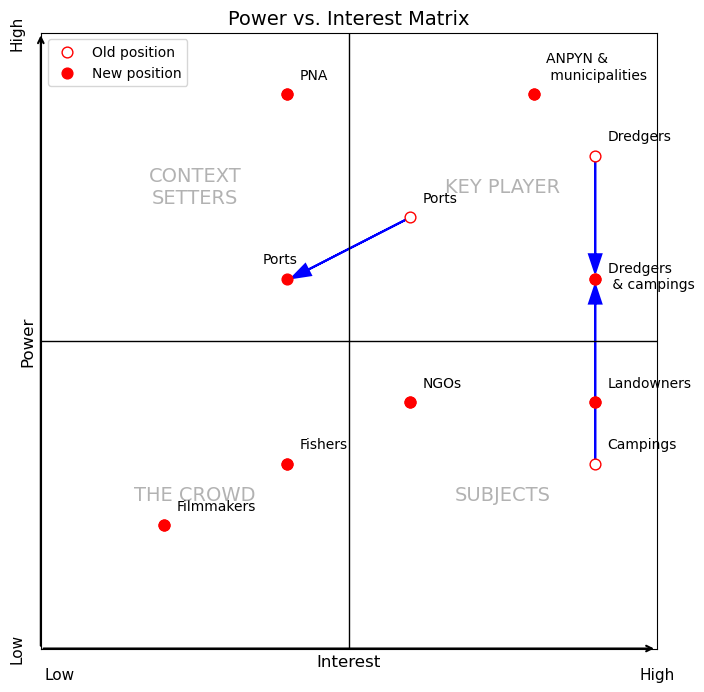
\includegraphics[width=0.65\linewidth]{figures/ch3/NewPowerVSInterest.png}
    \caption{Updated Power vs. Interest}
    \label{fig:power-interestNEW}
\end{figure}

In Figure \ref{fig:power-supportNEW}, the updated power vs. opposition-support-matrix can be found. The powers are updated in the same way as in Figure \ref{fig:power-interestNEW} and the degree of opposition was changed for the landowners and campings. From the interviews, many concerns about the dredging operations arose, such as sound pollution and erosion. Many voiced their opposition to the dredging clearly, which is why these stakeholders were moved to the left on the opposition/support scale. For the dredgers and ports, the same degree of support still holds, for monetary reasons. The municipality is opposed to the dredging, as can be seen from the mayor's statements on the discontinuation of dredging.

\begin{figure}[H]
    \centering
    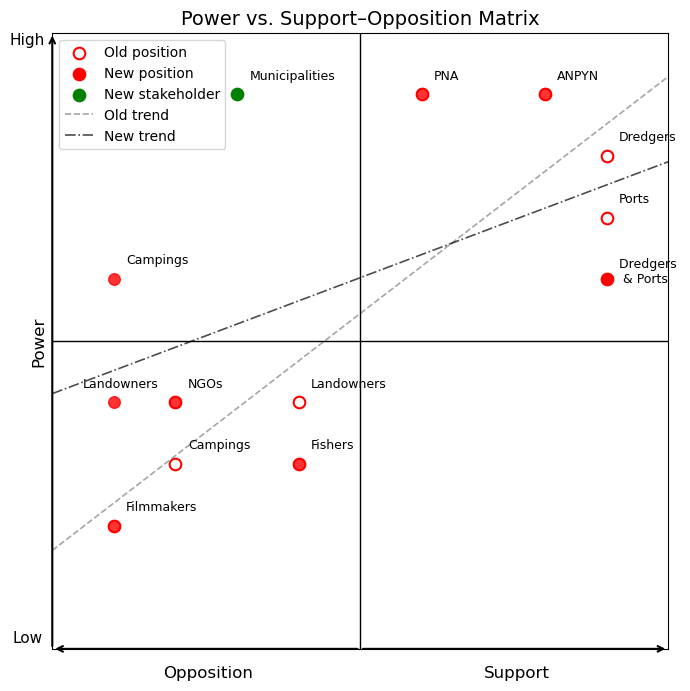
\includegraphics[width=0.65\linewidth]{figures/ch3/NewPowerVSSupport.png}
    \caption{Updated Power vs. Opposition-Support}
    \label{fig:power-supportNEW}
\end{figure}

In Figure \ref{fig:power-supportNEW}, it can be seen that the new trend is flatter than the original one. This is a consequence of the fact that dredging operations have not increased in recent years, as opposed to the expectation, and have in fact been completely stopped on the Ibicuy.
\chapter{Sand extraction}
Sand extraction in the Lower Paraná Delta occurs both on land and in the river. Therefore, dredging activities as well as dry sand mining are considered. The purpose of this chapter is to make an assessment of extraction quantities and evaluate the relative importance of the both types of sand extraction. 

\section{Dredging activities}
This section describes the relevance of dredging to the sediment balance of the designated area, by an estimation of the dredging quantities in the river. This will be done by analysing AIS data and extraction permits that were submitted to INA.

\subsection{Vessel positioning information (AIS)}
Using MarineTraffic it was found that two dredgers are operating on the Paraná Guazú between Ibicuy and Brazo Largo: the Comercio Segundo and the E.M. Arroyo N1. The Comercio Segundo has a length of 30 m, a width of 7 m, a draft of 1.3 m, and an approximate cargo hold of 195 m\textsuperscript{3}. The E.M. Arroyo N1 has a length of 39 m, a width of 8 m, a draught of 2.8 m and an approximate cargo hold of 476 \,m\textsuperscript{3}. Using a sand to water ratio of 3:1 for the dredged slurry, the amount of sand dredged is 150 \,m\textsuperscript{3} and 360 \,m\textsuperscript{3} respectively per cargo. The tracks of the two vessels obtained from MarineTraffic are shown in Figure \ref{fig:track_cs} and Figure \ref{fig:track_em}.

\begin{figure}[H]
    \centering
    \begin{minipage}{0.48\textwidth}
        \centering
        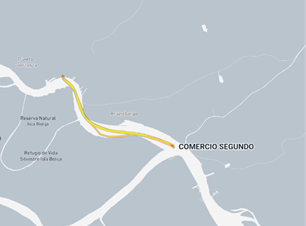
\includegraphics[width=\linewidth]{figures/ch5/Track_CS.png}
        \caption{Track of the \textit{Comercio Segundo}}
        \label{fig:track_cs}
    \end{minipage}\hfill
    \begin{minipage}{0.48\textwidth}
        \centering
        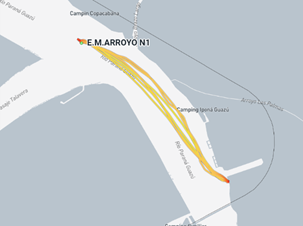
\includegraphics[width=\linewidth]{figures/ch5/Track_EM.png}
        \caption{Track of the \textit{E.M. Arroyo N1}}
        \label{fig:track_em}
    \end{minipage}
\end{figure}

The AIS data for these two vessels is obtained from MyShipTracking, which is used to determine the location of the dredging and the average number of trips. The dredging location of the two vessels is shown in Figure \ref{fig:dredging_coordinates}. It can be seen that both dredgers operate in the same area. This can be explained by the bathymetry shown in Figure \ref{fig:bathymetry}, which shows a reduced depth near the junction of the two navigable channels. At this location the flow velocity is lower, causing sediment to settle and thus creating a sandbar. From the AIS data it was concluded that both dredgers make three trips per day.

\begin{figure}[H]
    \centering
    \begin{minipage}{0.48\textwidth}
        \centering
        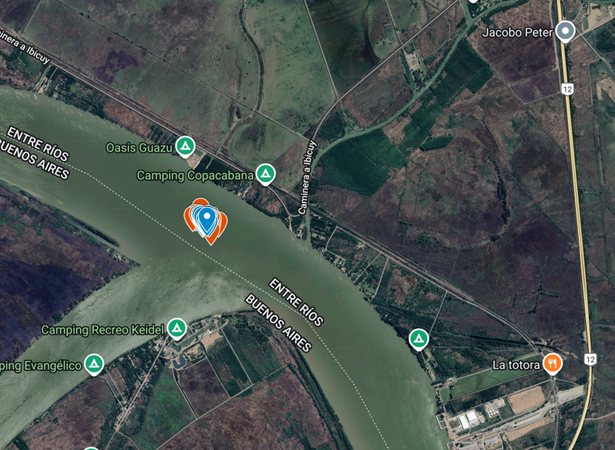
\includegraphics[width=\linewidth]{figures/ch5/Dredging_coordinates.png}
        \caption{Dredging location}
        \label{fig:dredging_coordinates}
    \end{minipage}\hfill
    \begin{minipage}{0.48\textwidth}
        \centering
        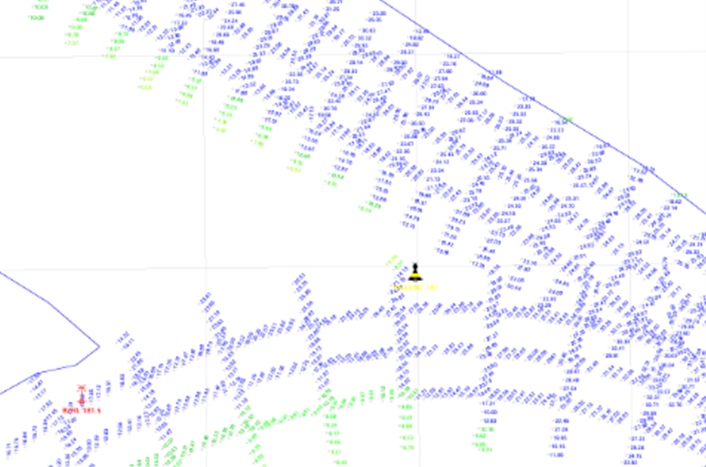
\includegraphics[width=\linewidth]{figures/ch5/Bathymetry.png}
        \caption{Bathymetry}
        \label{fig:bathymetry}
    \end{minipage}
\end{figure}

In the Rio Talabera, a side branch connecting to the Paraná Guazú, a third dredger is extracting sand. The Altair is a dredging vessel with a length of 66 m, a width of 11 m, a draught of 1.5 m and an approximate cargo hold of 750 \,m\textsuperscript{3}. Using the same sand to water ratio of 3:1 this gives 560 \,m\textsuperscript{3} of sand per cargo. Using MarineTraffic it was found that the Altair makes 3 trips per day on average. Figure \ref{fig:Altair_track} shows the its track and the location at which it halts to extract sand. For all three vessels that were identified in the study area, the estimated volume of sand extracted per month is displayed in Table \ref{tab:sand_volume}.

\begin{figure}[H]
    \centering
    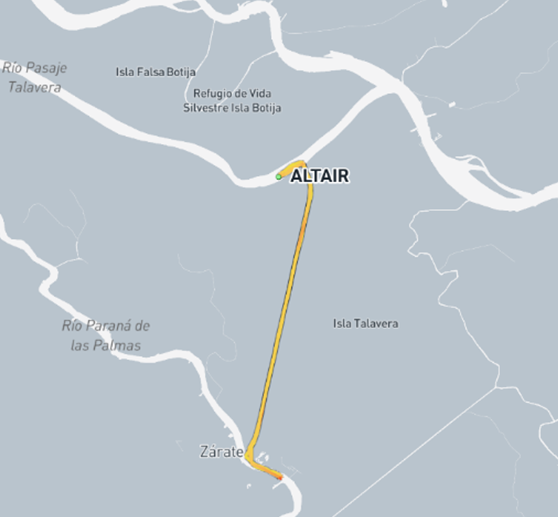
\includegraphics[width=0.5\linewidth]{figures/ch5/Track_Altair.png}
    \caption{Track of the Altair}
    \label{fig:Altair_track}
\end{figure}


\begin{table}[h!]
\centering
\begin{tabular}{lrrrr}
\hline
\textbf{Vessel} & \textbf{Cargo hold [\,m\textsuperscript{3}]} & \textbf{Sand volume [\,m\textsuperscript{3}]} & \textbf{Trips per day} & \textbf{Volume per month [\,m\textsuperscript{3}]} \\
\hline
Comercio Segundo & 195 & 150 & 3 & 9000 \\
E.M. Arroyo N1 & 476 & 360 & 3 & 21600 \\
Altair & 750 & 560 & 3 & 33600 \\
\hline
\end{tabular}
\caption{Sand transport details per vessel.}
\label{tab:sand_volume}
\end{table}

\subsection{Extraction permits}
A total of 33 permits were collected for the Paraná Guazú and 43 for the Ibicuy. On the Paraná Guazú, four permits were issued for channel maintenance, while the remainder concerned sand extraction. For the Ibicuy, all permits were related to extraction activities. The analysis shows that the requested volumes in the Ibicuy are considerably larger than those in the Paraná Guazú, even though the section of the Ibicuy considered here is much shorter in length: Paraná Guazú stretches from km 124.0 to km 232.0, Ibicuy from km 232.0 to approximately km 249.0 for the area of interest \autocite{administraciongeneraldepuertoss.a.u.AGPComenzoBatimetria2023}.

It is important to note that the end dates of contracts are unknown. While the requests specify monthly dredging quantities, they do not indicate the duration of the works. As a result, a detailed quantitative assessment cannot be made. For the present analysis, all requests with fixed monthly volumes are assumed to extend over 12 months. The second assumption is to record a single value for the requested volume, when information about monthly or yearly occurrence is lacking. This allows for a comparison between the two river sections of yearly extraction volumes, as shown in Figure \ref{fig:yearly dredging volumes}. As mentioned, sand extraction activities on the Ibicuy are large compared to Paraná Guazú, with a maximum recorded yearly volume of almost $4 \cdot 10^6 ~m^3$.  

\begin{figure}[H]
    \centering
    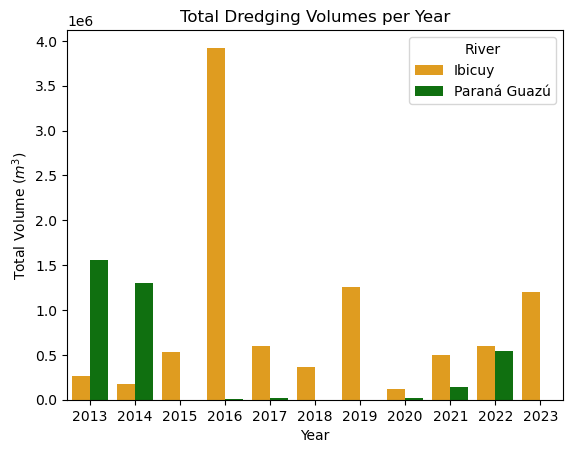
\includegraphics[width=0.50\linewidth]{figures/ch2/Dredging volumes permits.png}
    \caption{Yearly dredging volumes}
    \label{fig:yearly dredging volumes}
\end{figure}

\subsection{Estimated sand extraction}
This section draws a conclusion on the sand extraction volumes, such that an estimate is found to apply in the sediment balance. Based on the AIS data, permits and stakeholder interviews, the following uncertainties were considered in determining a representative value:

\begin{itemize}
    \item Not every vessel in the area is equipped with an AIS transponder, meaning that possibly not all active vessels were identified. However, the number of vessels as found by analysis of the AIS data was in agreement with the number of vessels observed during the fieldwork.
    \item No historical AIS data was available, such that the data was registered for only a short period of time.
    \item The extraction permits do not mention the duration of the contract.
    \item Whereas permits imply that most of the activity occurs on the Ibicuy, AIS data and fieldwork observations indicate that the activity on the Paraná Guazú is higher. 
    \item Stakeholders stress that activity on the Ibicuy has ceased, as described in Section \ref{subsec:dredging activities interviews}.
\end{itemize}

However, a rough estimate can be found by calculating the mean annual volume for the total system of interest (i.e., Ibicuy and Paraná Guazú) based on the extraction permits. To make a comparison with the monthly values in Table \ref{tab:sand_volume}, this yearly value is reduced to a monthly value by dividing by 12 months. The former approach yields the following value for dredged sand volumes:

\begin{equation}
    V_{sand,yearly} = 1193923 ~m^3
\end{equation}
\begin{equation}
\label{eq:monthly extraction}
    V_{sand,monthly} = \frac{V_{sand,yearly}}{12} \approx 100000 ~m^3
\end{equation}

Summation of the monthly volumes in Table \ref{tab:sand_volume} gives a monthly total of $64200 ~m^3$. Considering that not all vessels have AIS transponders, a conservative estimate of $V_{sand,monthly}$ will be used as calculated in Equation \ref{eq:monthly extraction}.

\section{Dry sand mining}
As mentioned in chapter \ref{chapter:stakeholders}, many stakeholders stressed the relevance of dry sand mining related to fracking for the lower delta region. In this section, context to these claims is given. The history and development of fracking in Argentina is discussed, followed by the related sand mining. Then, geological properties of the area of interest are looked into as well as the characteristics of dry sand used in fracking. Finally, the effects of dry sand mining are discussed and recommendations plus mitigation strategies are given.

\subsection{Fracking in Argentina}
\label{sec: fracking in argentina}
For much of its history, Argentina was regarded as a modest oil producer, struggling to meet its own energy demands. This perception shifted with the 2010 discovery of the Vaca Muerta shale formation, located in the Neuquén basin in Patagonia. The Argentine energy company YPF then identified approximately 150 million barrels of recoverable oil in the field, which was regarded as a new source of hope for economic stability by some, among whom was the president \autocite{kraussArgentinaHopesBig2011}.

The discovery was followed by significant foreign investment. More exploration was done and now it is clear that Argentina possesses the world’s fourth-largest shale oil and second-largest shale gas reserves \autocite{internationaltradeadministrationArgentinaCountryCommercial2025}. Today, around thirty companies hold licenses to exploit various areas of the Vaca Muerta basin. The biggest operator is a consortium of YPF, a majority state-owned Argentine energy company, and Chevron, an American energy company. Other players are Tecpetrol, Total, Dow Petrochemical, Petronas, Shell, Gazprom, and ExxonMobil \autocite{fogliaSedArena2023}.

The Nuequén basin is located in the provinces of Neuquén, Mendoza, and Río Negro in the South of Argentina and has been an important basin for oil and gas since more than a century. Production started in 1918 and in 2004, 45\% of Argentinian oil production and 61\% of its gas production came from this area \autocite{u.s.energyinformationadministrationTechnicallyRecoverableShale2013}. This was done through conventional methods, but after the discovery of the Vaca Muerta shale basin, fracking has become increasingly important for the region and the country. The Vaca Muerta shale consists of finely-stratified black to dark grey shale and lithographic lime-mudstone and is 60 to 520 m thick. Estimates are that the formation contains 16 billion barrels of technically recoverable oil and 8722 billion cubic metres of technically recoverable gas \autocite{u.s.energyinformationadministrationTechnicallyRecoverableShale2013}. Since Vaca Muerta is a shale reservoir, all oil and gas from this deposit is extracted by fracking.

As can be seen in figure \ref{fig:oilgasprod}, oil production in Argentina has been steadily increasing since 2020, driven by increased production of the Vaca Muerta formations. After the exploration in 2010, oil from Vaca Muerto as a share of total Argentinian oil production has increased from virtually 0\% to 55\% today. Further, Vaca Muerta now accounts for 47\% of gas supply \autocite{internationaltradeadministrationArgentinaCountryCommercial2025}.

\begin{figure}[H]
    \centering
    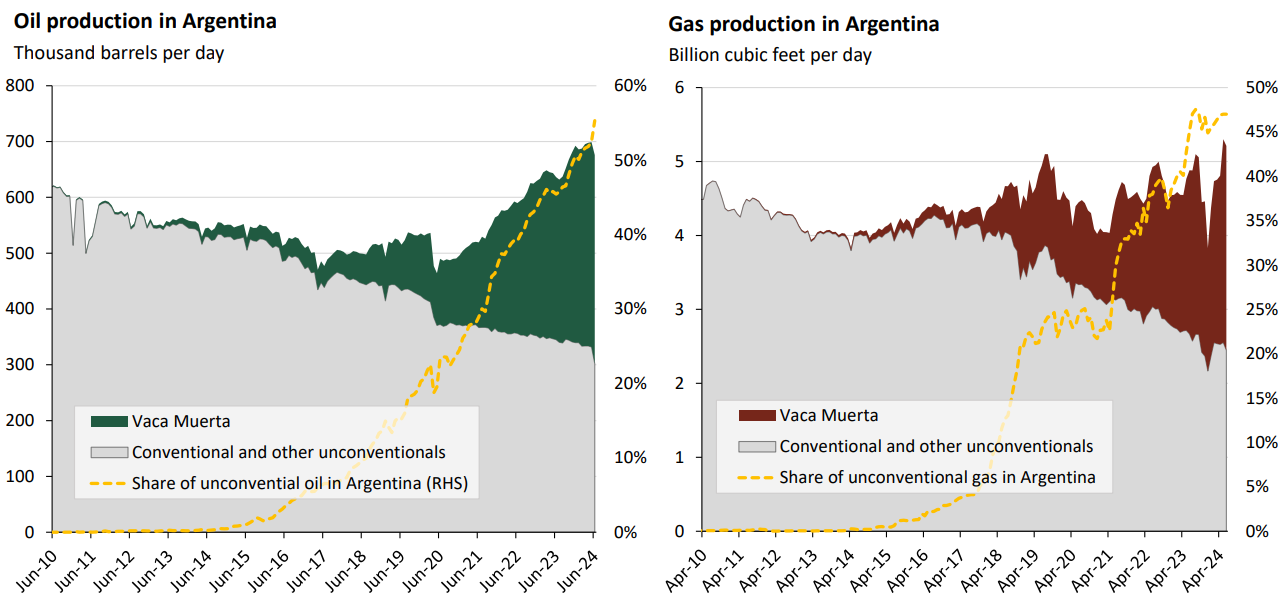
\includegraphics[width=1\linewidth]{figures/ch9/oilgasproduction.png}
    \caption{Oil and gas production in Argentina \autocite{internationaltradeadministrationArgentinaCountryCommercial2025}}
    \label{fig:oilgasprod}
\end{figure}

The numbers in figure \ref{fig:oilgasprod} help explain why fracking in the Neuquén basin is viewed by some as critical to the development of Argentina's economy. In fact, the Government of Argentina still views the oil and gas sector as a crucial part of its economy, by driving exports as well as generating foreign currency and investment. It also becomes clear that, considering the volumes present in the reserves, even more gas and oil could still be extracted.

\subsection{Theoretical background: fracking}
In the 1970's, geologists became increasingly aware that large volumes of gas existed in low-permeability sandstones. However, conventional methods did not allow for economic extraction of gas from these `tight reservoirs' \autocite{lawGasTightReservoirs1992}. Hydraulic fracturing, or fracking, a method first tested in 1947 and applied on a large scale for the first time in the 1970's, is used to extract oil and natural gas from these low-permeability rock formations, such as shale \autocite{denchakFracking1012019}.

The technique begins by drilling a long vertical well. As soon as the desired rock formation is reached, drilling gradually turns horizontal and steel pipes called `casings' are inserted into the well. Small holes are perforated in the casing and then fracking fluid is pumped in at a pressure high enough to create new fractures or open existing ones in the surrounding rock. This allows previously unavailable oil or gas to flow to the surface \autocite{denchakFracking1012019}.

The fracking fluid contains as much as 97 percent water, but also always contains proppants. These are small, solid particles that keep the fractures in the rock formation open after the pressure from injection is removed. Sand, or more specifically silica sand, is the most widely-used proppant in the fracking industry \autocite{denchakFracking1012019}. Sand is thus an essential substance to keep the drilled pores open and to allow for the fossil fuels to flow out.

\subsection{Sand mining practices}
The sand used in fracking is mined or imported. In figure \ref{fig:sanddiagram}, the mined silica sand masses as well as the imported masses are given for Argentina. This includes sand used for fracking but also other purposes.

\begin{figure}[H]
    \centering
    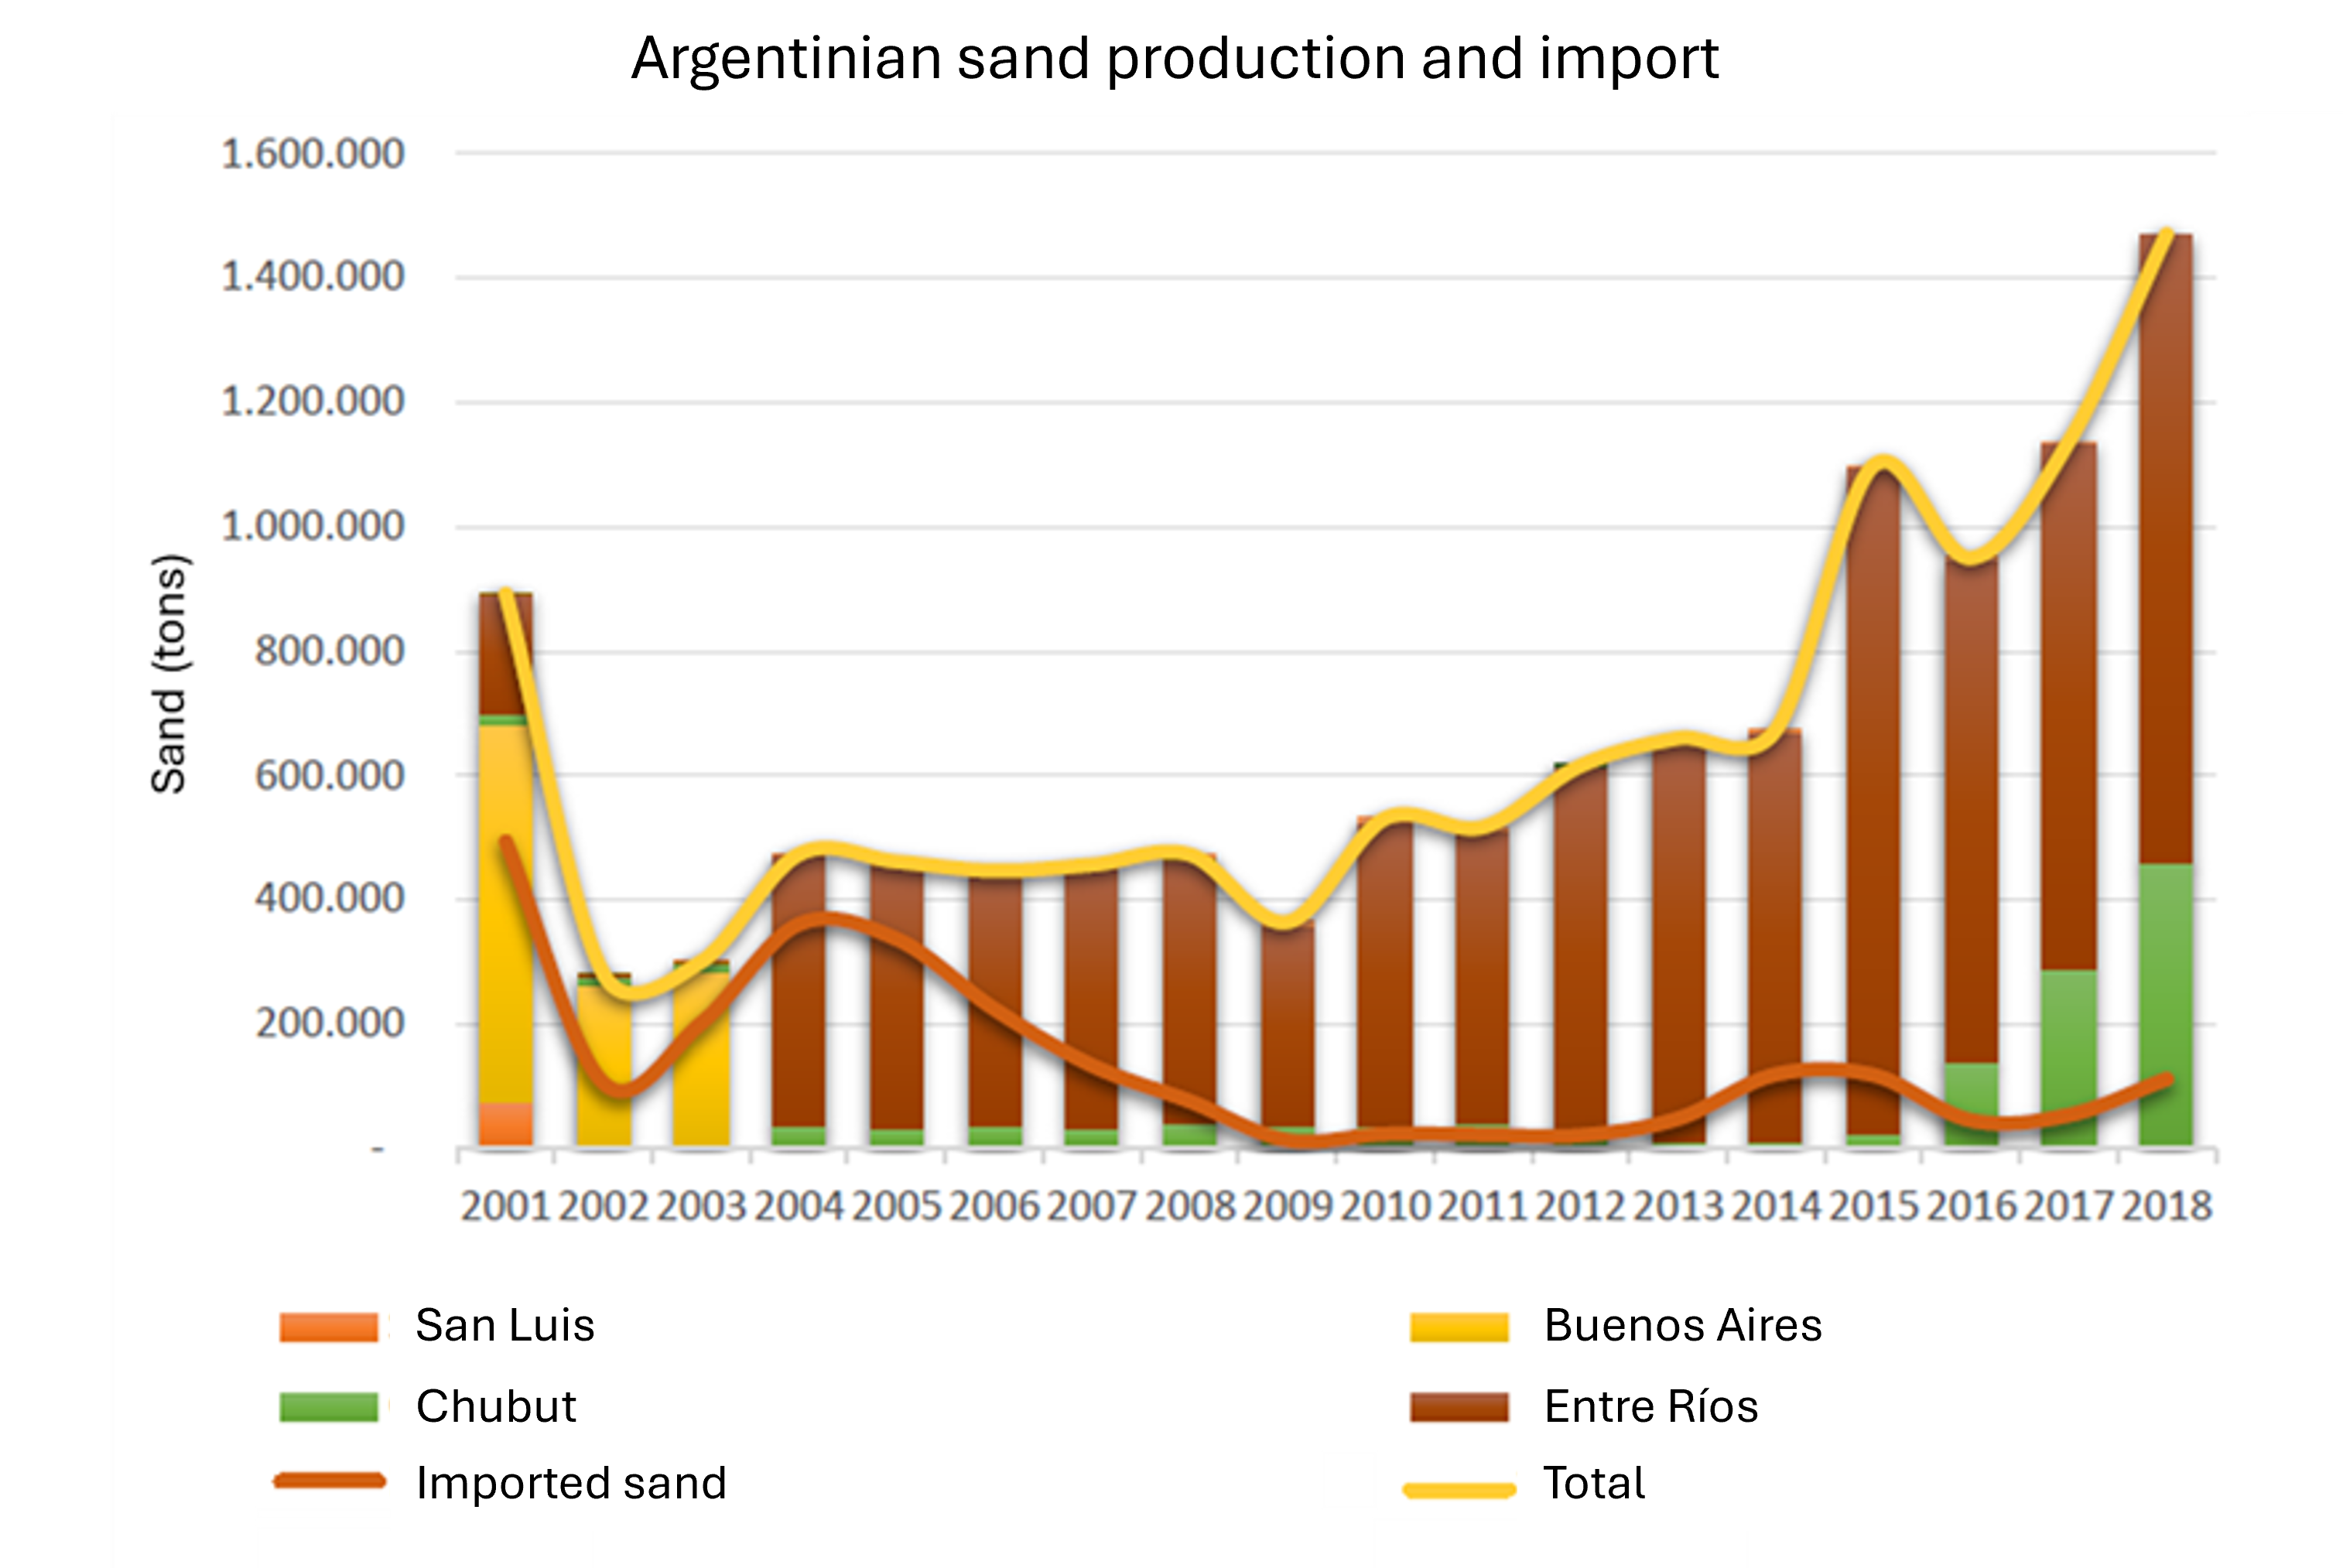
\includegraphics[width=1\linewidth]{figures/ch9/Sandgraphquantities.png}
    \caption{Quantities of sand mined in Argentine provinces, adapted from \autocite{secretariadepoliticamineraArenasParaFracking2019}}
    \label{fig:sanddiagram}
\end{figure}

In 2018, approximately 1.5 million tons of sand was produced and imported in Argentina, with more than 90\% of used sand from national origin. Of the nationally mined sand, 69\% had its origin in Entre Ríos \autocite{secretariadepoliticamineraArenasParaFracking2019}. Specific numbers for the period after are unavailable, but in 2020, the amount of sand needed in Argentina was 3.5 million tons \autocite{novasImpactoAmbientalOculto2022}.

Historically, silica sand was used as a raw material for the glass industry but since the introduction of fracking, sand miners have found a new purpose for their product. The exact volumes of sand used for fracking versus the volumes used for other purposes are unknown. However, as can be seen in figure \ref{fig:sanddiagram}, the upgoing trend in sand production can be observed only for the past years, after the discovery of Vaca Muerta.

\subsection{Sand mining in the lower delta}
During the fieldwork and by using satellite data, the locations of sand mines in the lower delta were identified. A total of 11 locations were found, 10 of which fall within the department of Islas del Ibicuy. In figure \ref{fig:sandminemap} the locations are shown and in figure \ref{fig:sandminessatellite}, the aerial view is given for three sand mines in the department of Ibicuy.

\begin{figure}[H]
    \centering
    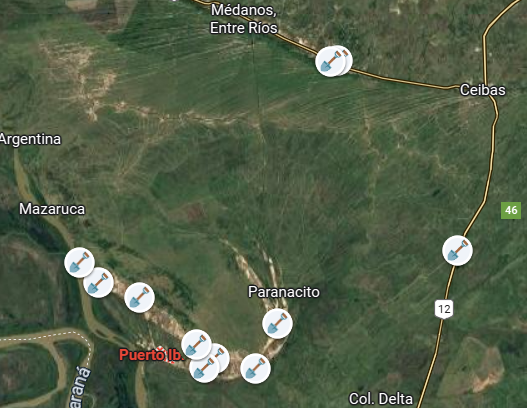
\includegraphics[width=0.6\linewidth]{figures/ch9/SandMap.png}
    \caption{The identified locations of sand mines}
    \label{fig:sandminemap}
\end{figure}

\begin{figure}[H]
    \centering
    \includegraphics[width=1\linewidth]{figures/ch9/Sandminessatellite.png}
    \caption{Examples of sand mines in the department of Ibicuy}
    \label{fig:sandminessatellite}
\end{figure}

Of all departments where sand mining takes place, the most intense activities are carried out in Ibicuy. Previous reports estimate that 1.250.000 tons of sand were mined in Ibicuy alone in 2022 \autocite{fogliaSedArena2023}. This number is comparable to the total national sand mining volume in 2018.

In Ibicuy, Cristamine, Aresil S. A., YPF, La Chola II, NRG Argentina, San Marcos Trading, and QSand are among the companies that operate sand mining facilities. Sand mining companies that have been around for longer originally only sold their product to the ceramics and glass industry, but at present many of them exclusively sell to the oil sector. Other companies only opened mines after the demand for fracking sand started to rise. An example is La Chola II, a company with 50 years of experience in river sand mining, that opened a dry sand mine in 2016. This is Silicatos Islas del Ibicuy and from here they transport sand to YPF, the biggest player in Argentina's fracking industry \autocite{fogliaSedArena2023}.

Mined sand gets transported by trucks to Añelo, a town in Neuquén that forms the heart of the Vaca Muerta fracking activities. The route from Ibicuy to Añelo is 1283 km long and takes around 20 hours, including a 2 hour delay for handling of goods \autocite{secretariadepoliticamineraArenasParaFracking2019}. The route is indicated in figure \ref{fig:sandroute}. 

\begin{figure}[H]
    \centering
    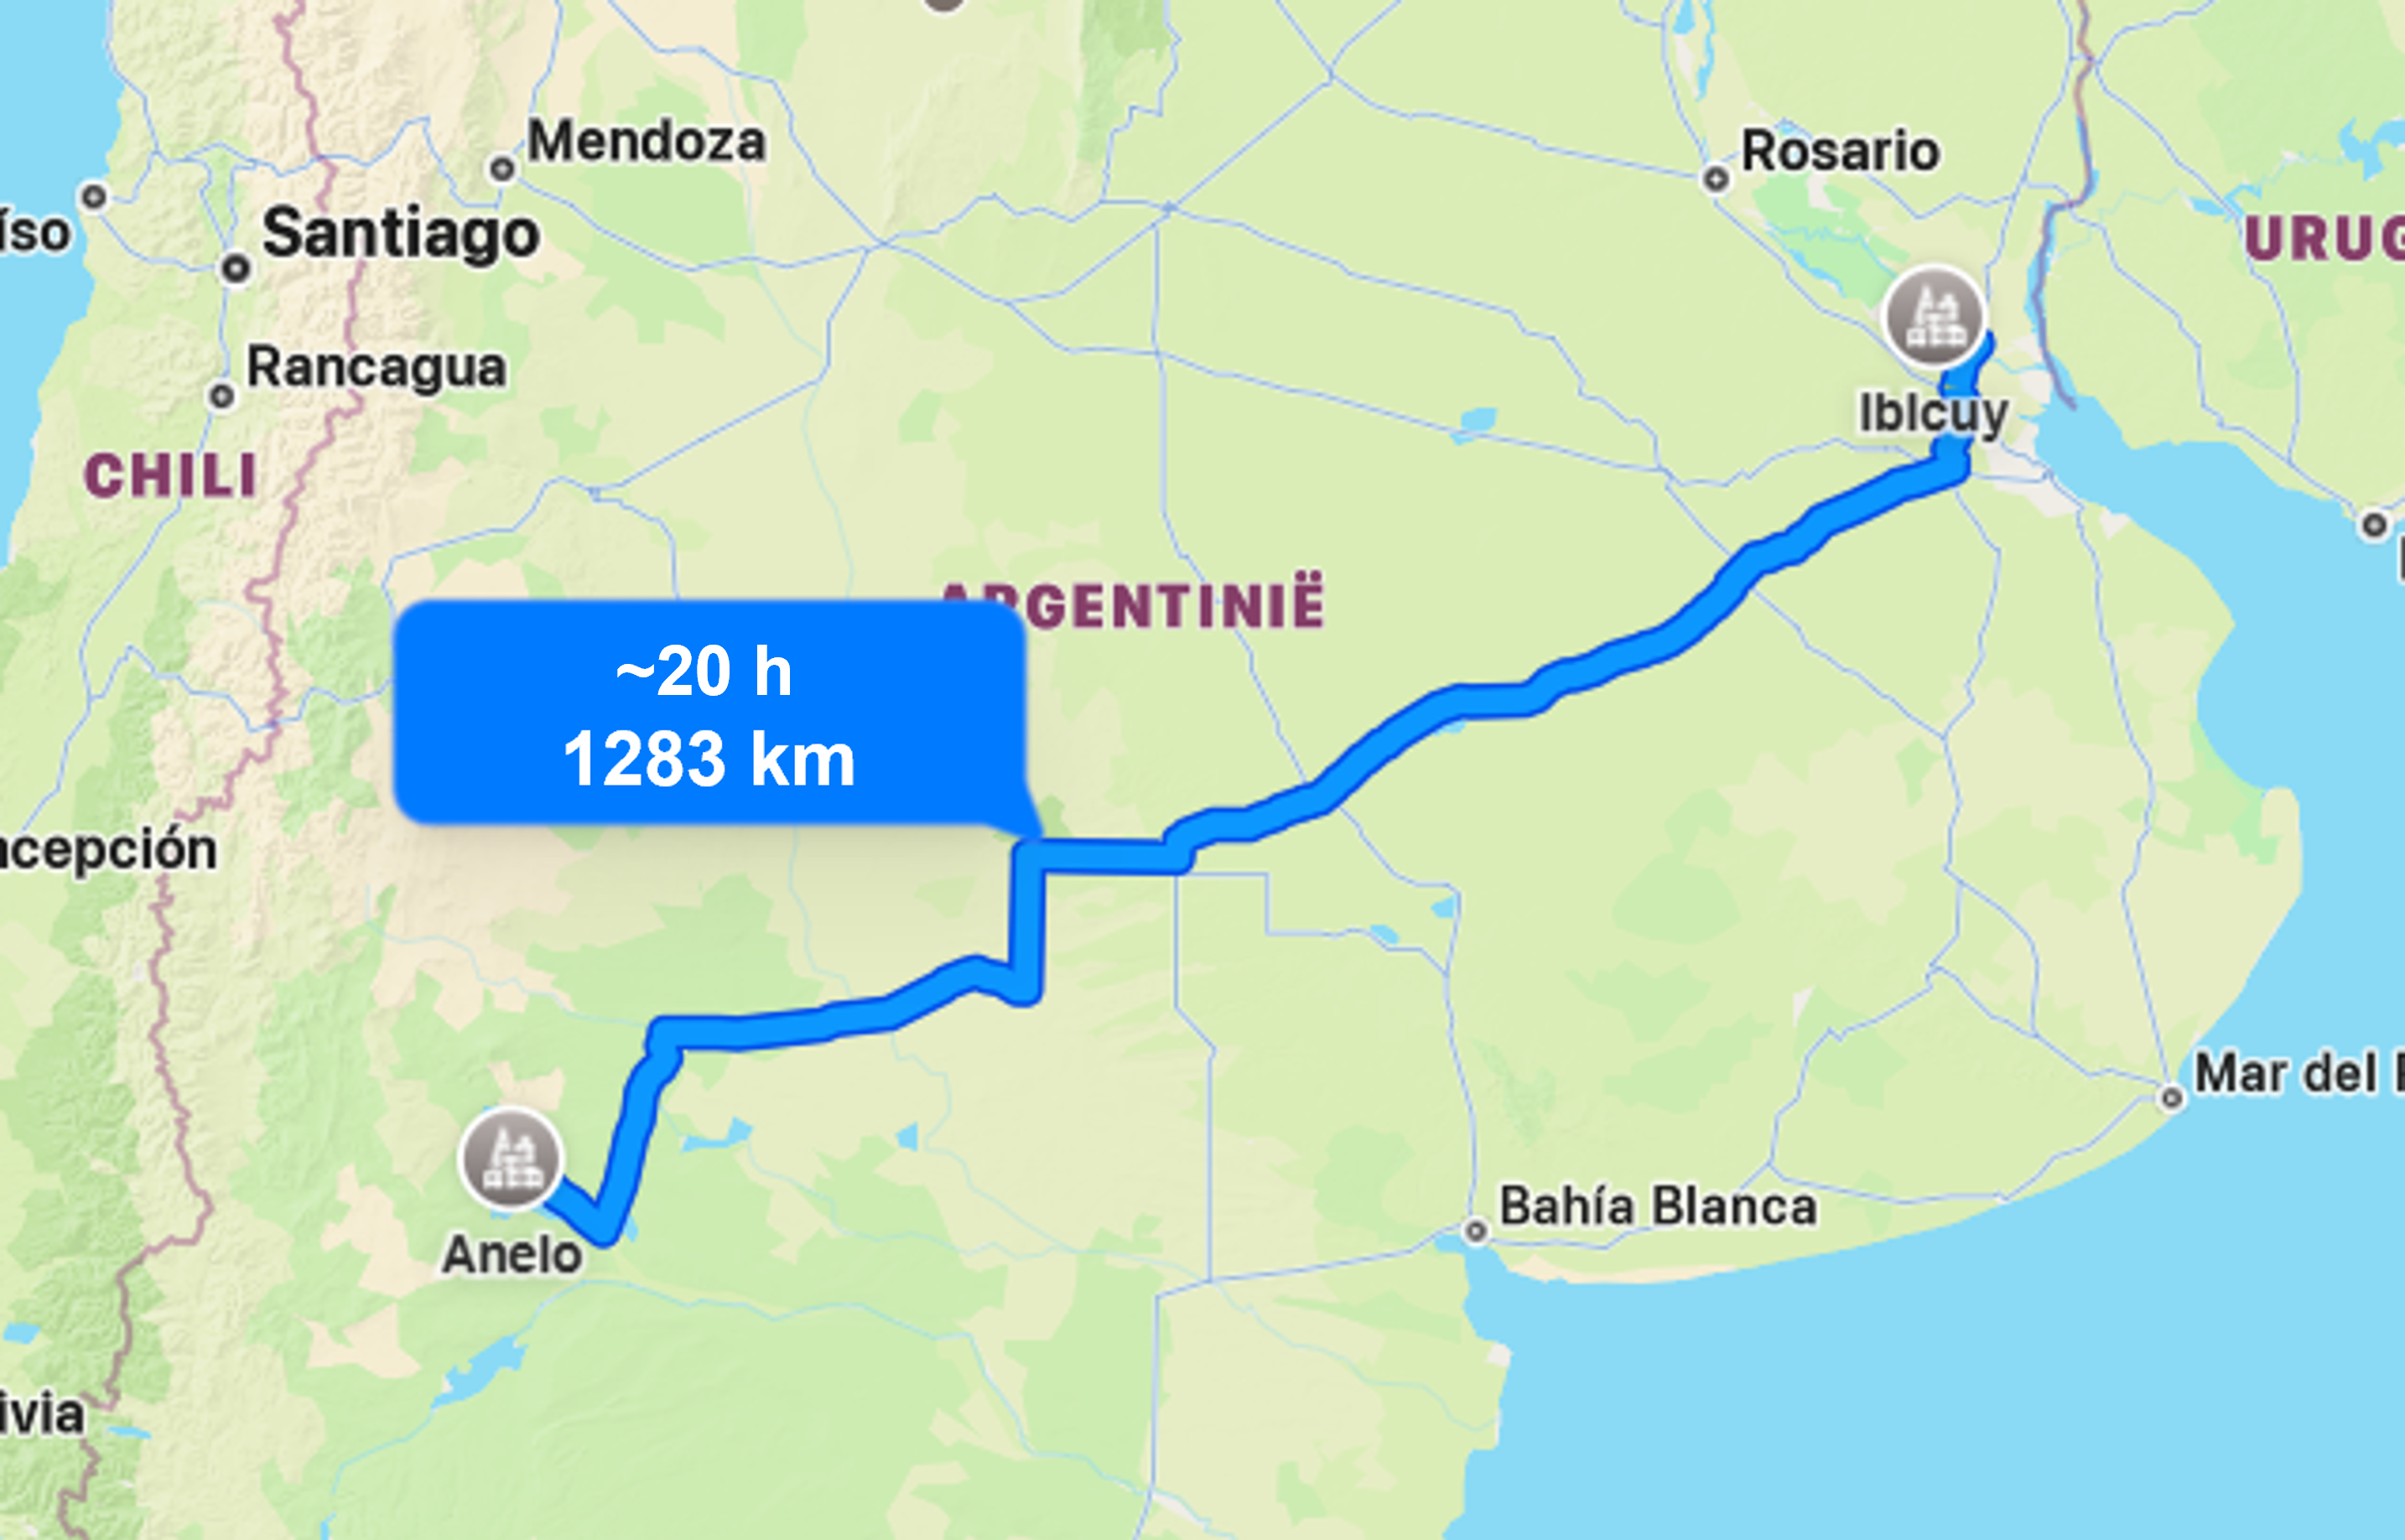
\includegraphics[width=0.6\linewidth]{figures/ch9/Routesand.png}
    \caption{The route from Ibicuy to Añelo}
    \label{fig:sandroute}
\end{figure}

\subsection{Geological conditions} \label{par:geology}
To better understand the dry sand mining activities, the characteristics of the subsoil in the lower delta were researched. This section intends to combine all the available information regarding the subsoil in the investigation area.

\subsubsection{The geology of a delta}
A delta is a landscape formed at the mouth of a river where the water eventually runs into the ocean. At a delta, the water's velocity decreases which gives floating particles in the delta the change to settle. Among these floating particles are gravels, sands and clays, descending in particle size. The particles are formed by erosion of stone. The origin of the particles in the Parana river are the Andes mountains. 
Besides that, deltas are also characterized by high vegetation growth. When this vegetation dies, the organic material will change into peat due to the governing pressures. So, in a delta one expects to find relatively soft soils (sands) and very soft soils (clay and peat).

\subsubsection{Geological cross section}
A study conducted by \citeauthor{cavallottoEvolucionCambiosAmbientales2005} led to a morphological map of the Paraná delta. In the study, a more detailed geological profile was made for two cross sections, one of which is relevant to the area of interest. The cross section along with the area of interest is shown in figure \ref{fig:crosssectiongeo}.

\begin{figure}[H]
    \centering
    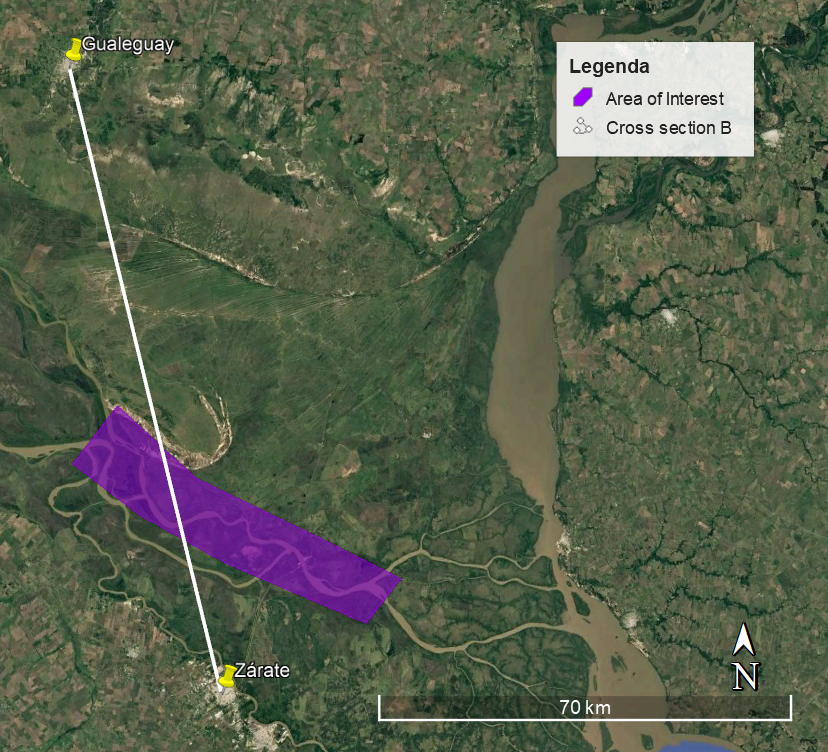
\includegraphics[width=0.75\linewidth]{figures/ch9/CrossSectionB.png}
    \caption{Cross section}
    \label{fig:crosssectiongeo}
\end{figure}

The geological profile of the cross section is shown in figure \ref{fig:geolprofile}. As can be seen in the figure, the taken cross section was around 80 km long. Of this, 15 km falls inside the area of interest, this zone is marked with purple.

\begin{figure}[H]
    \centering
    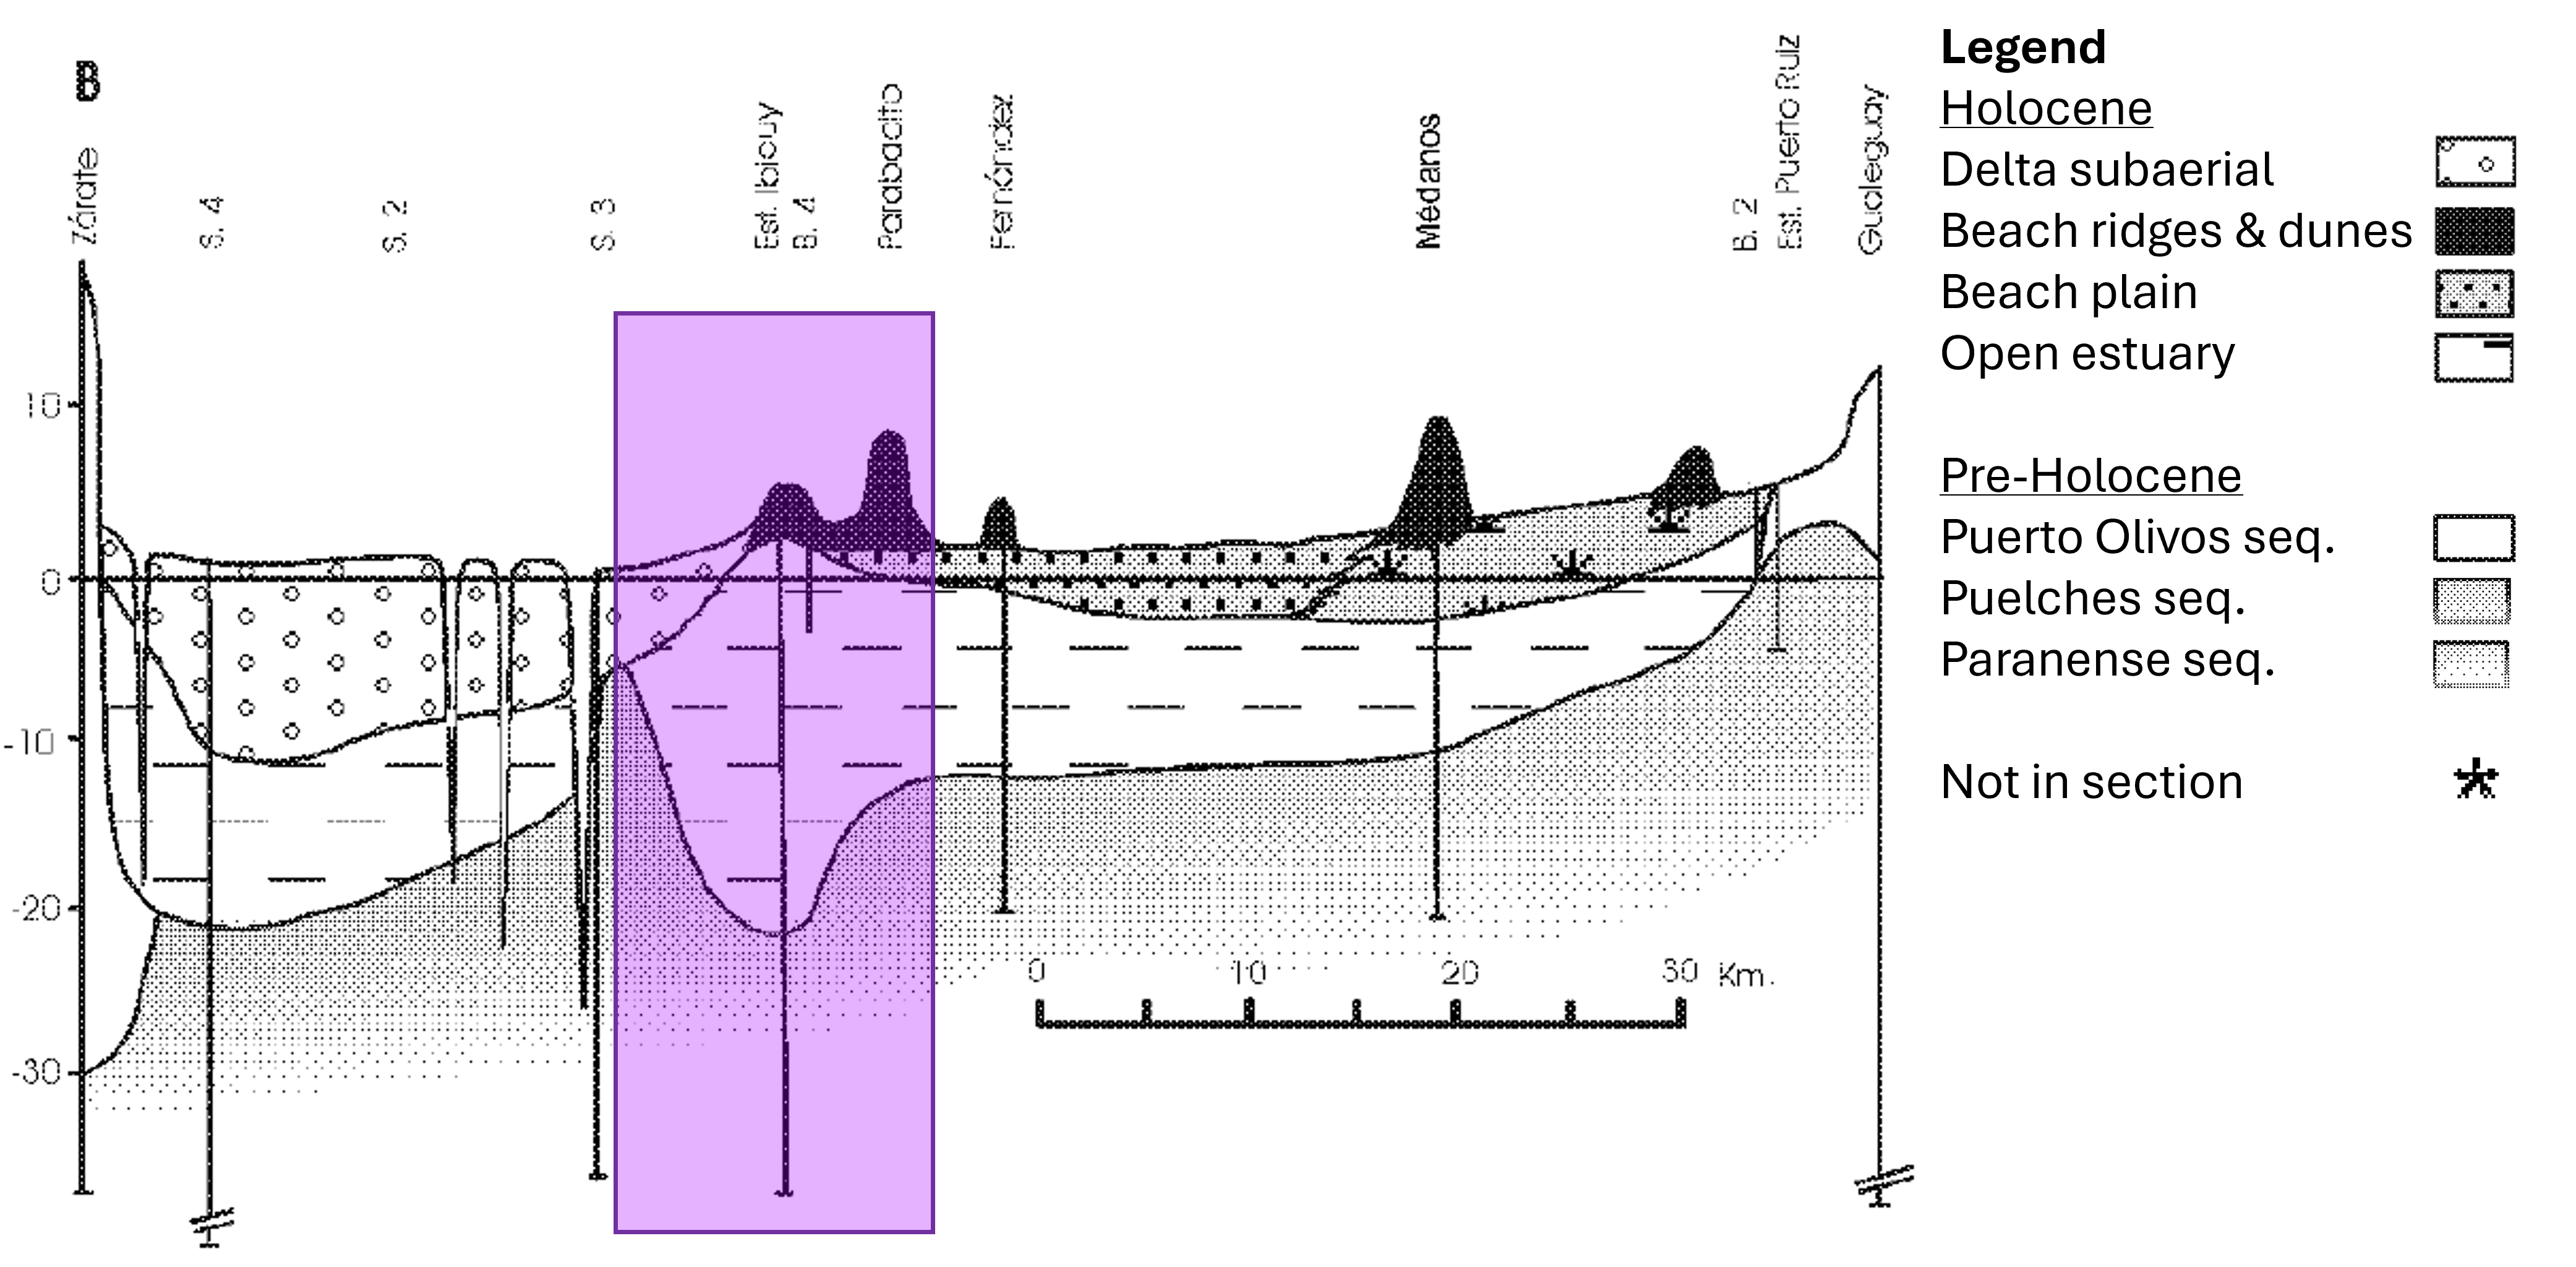
\includegraphics[width=1\linewidth]{figures/ch9/CrossSectionBResults.png}
    \caption{Geological profile of cross section \autocite{cavallottoEvolucionCambiosAmbientales2005}}
    \label{fig:geolprofile}
\end{figure}

\begin{itemize}
    \item Beach ridges \& dunes: This layer consists of ridge-like beach deposits overlain by dunes. The beach deposists have a maximum thickness of 2 m and are composed mainly of well-sorted fine to medium sands with shell fragments. Light minerals represent 97.8\% of the sand, almost all of which is quartz \autocite{cordiniContribucionConocimientoGeologia1949}. Radiocarbon dating indicates the deposits formed about 6,400–5,500 years ago, during the mid-Holocene. The ridges represent berm deposits formed by coastal progradation toward the northwest, driven by southeast winds and littoral drift.
    The dunes are up to 11 meters high, especially near Ibicuy, where dune elevations range from 9 to 11 meters and extend 1–2.5 km wide. The dunes consist of well-sorted, fine brown sands composed mostly of quartz (>99\%), with minor feldspars and heavy minerals such as magnetite, zircon, staurolite, and kyanite \autocite{cordiniContribucionConocimientoGeologia1949}. Thermoluminescence dating shows ages between ~2,800 and <500 years old, indicating several phases of dune formation. Their greatest development on the southeast side shows that, like the underlying beach ridges, they were shaped by southeast winds and continue to be reworked by modern activity \autocite{cavallottoEvolucionCambiosAmbientales2005}.

    \item Beach plain: The Beach Plain Facies consist of a series of closely spaced beach ridges formed during phases of shoreline retreat and sediment accumulation. The deposits are composed of fine to very fine sands, moderately to well sorted, dominated by quartz (85–90\%) with minor feldspars and few heavy minerals \autocite{cordiniContribucionConocimientoGeologia1949}. Radiocarbon testing suggests ages between ~2,600 and 1,800 years. The presence of both estuarine shells and freshwater species indicates a transition from estuarine to fluvial conditions as river influence increased \autocite{cavallottoEvolucionCambiosAmbientales2005}.

    \item Delta subaerial: The subaerial facies of the Paraná Delta developed through the deposition of silty-sandy sediments delivered mainly by the Paraná Guazú and Paraná de las Palmas \autocite{cavallottoEvolucionCambiosAmbientales2005}. These deposits occur at elevations between 2 m and sea level, with a maximum thickness of 12 m. This is the layer that is drained.
    Mineralogical analyses show a predominance of quartz with minor plagioclase and K-feldspar, plus heavy minerals such as magnetite, hematite, garnet, zircon, tourmaline \autocite{cavallottoEvolucionCambiosAmbientales2005}. The age of the unit is debated: radiocarbon dates suggest origin dates between -150 BC and 180 AD, while other authors propose a later origin around 700–750 AD \autocite{cavallottoEvolucionCambiosAmbientales2005}.
    
    \item Open estuary: The open estuary sediments were deposited during postglacial sea-level rise and were formed at the freshwater–saltwater interface. At the time, seawater flooeded the Río de la Plata river valley \autocite{cavallottoEvolucionCambiosAmbientales2005}.
    These are olive-green clays to silty clays with thin fine-sand layers, scattered or concentrated shell beds, and fossil content confirming estuarine conditions. The unit is dated to the Holocene, with its base at ~6670 +/- 100 years BC, occurring between –22 and –0 m and reaching up to 20 m thick \autocite{vogelGroningenRadiocarbonDates1969}.
    
    \item Paranense sequence: During the Miocene, large portions of present-day Argentina, Uruguay, Paraguay, southern Brazil, and eastern Bolivia were covered by the Paranense Sea. This was a shallow sea that advanced from the Atlantic into the interior of South America . Its waters left behind marine sediments and fossils and this layer is now known as the Paranense depositional sequence \autocite{tineoReconstructingSouthAmerican2024}.
    
    It is composed mainly of siliciclastic sandstones, mudstones, and bioclastic beds, with thicknesses ranging from a few meters in outcrop to over 100 m. The lower part has mud-dominated offshore deposits with marine fossils, while the upper part is sandier. Studies link the deposits to the Late Miocene (ca. 9.5–6.7 Ma) \autocite{tineoReconstructingSouthAmerican2024}.
\end{itemize}

%Another study focuses on subsurface deposits from Diamante in Entre Ríos to San Fernando in the Buenos Aires province. Based on lithologic, clay mineral, radiocarbon, and outcrop data, the authors propose a depositional model for the region. This geological cross section is shown in figure \ref{fig:depmodel}. The purple area marks the area of interest for this research (Puerto Ibicuy).

%\begin{figure}[H]
%    \centering
   % 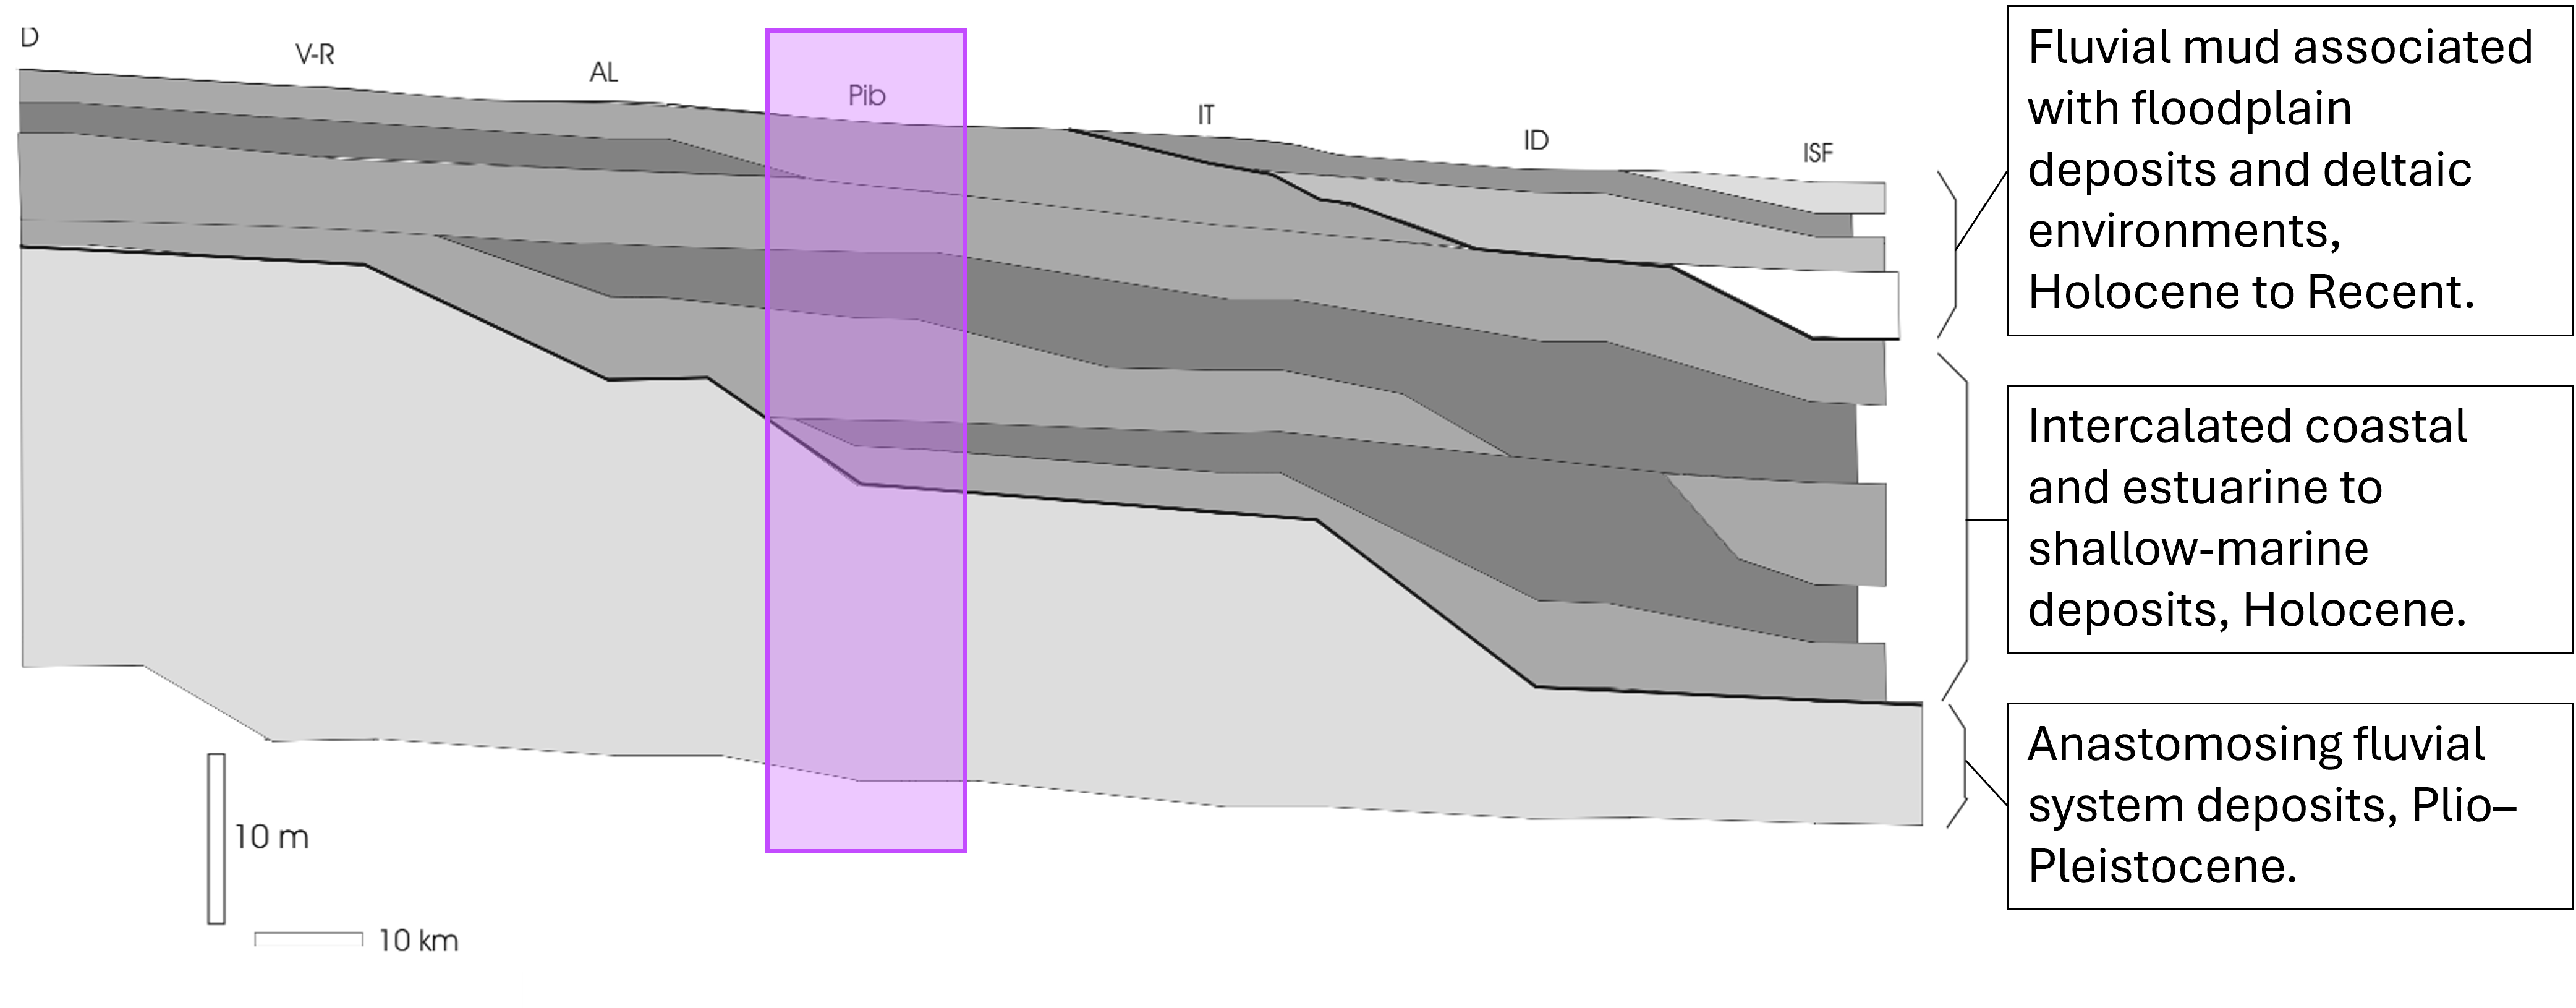
\includegraphics[width=1\linewidth]{figures/ch9/Crosssection2.png}
  %  \caption{Depositional model \autocite{amatoEstratigrafiaCuaternariaSubsuelo2009}}
  %  \label{fig:depmodel}
%\end{figure}

%As can be seen in the figure, the first layer consists of deltaic and flooplain deposits from the Holocene until recent times. This is in accordance with the geological profile as shown in figure \ref{fig:crosssectiongeo}. Underneath, holocene coastal/estuarine sediments can be found and below there are the Plio–Pleistocene fluvial deposits. The estuarine sediments can also be found in figure \ref{fig:crosssectiongeo}, but a different conclusion was reached for the final layer. \citeauthor{cavallottoEvolucionCambiosAmbientales2005} conclude that this is a pre-holocene marine deposit from the Miocene Paranense Sea, while here Plio–Pleistocene river deposits are placed below the Holocene sequence.

\subsubsection{Borehole}
In a study conducted by \citeauthor{amatoEstratigrafiaCuaternariaSubsuelo2009}, a number of boreholes were executed along the lower Paraná \autocite{amatoEstratigrafiaCuaternariaSubsuelo2009}. One of these boreholes was executed near the area of interest in Puerto Ibicuy. The borehole was interpreted and with this the following soil profile was made.

\begin{figure}[H]
    \centering
    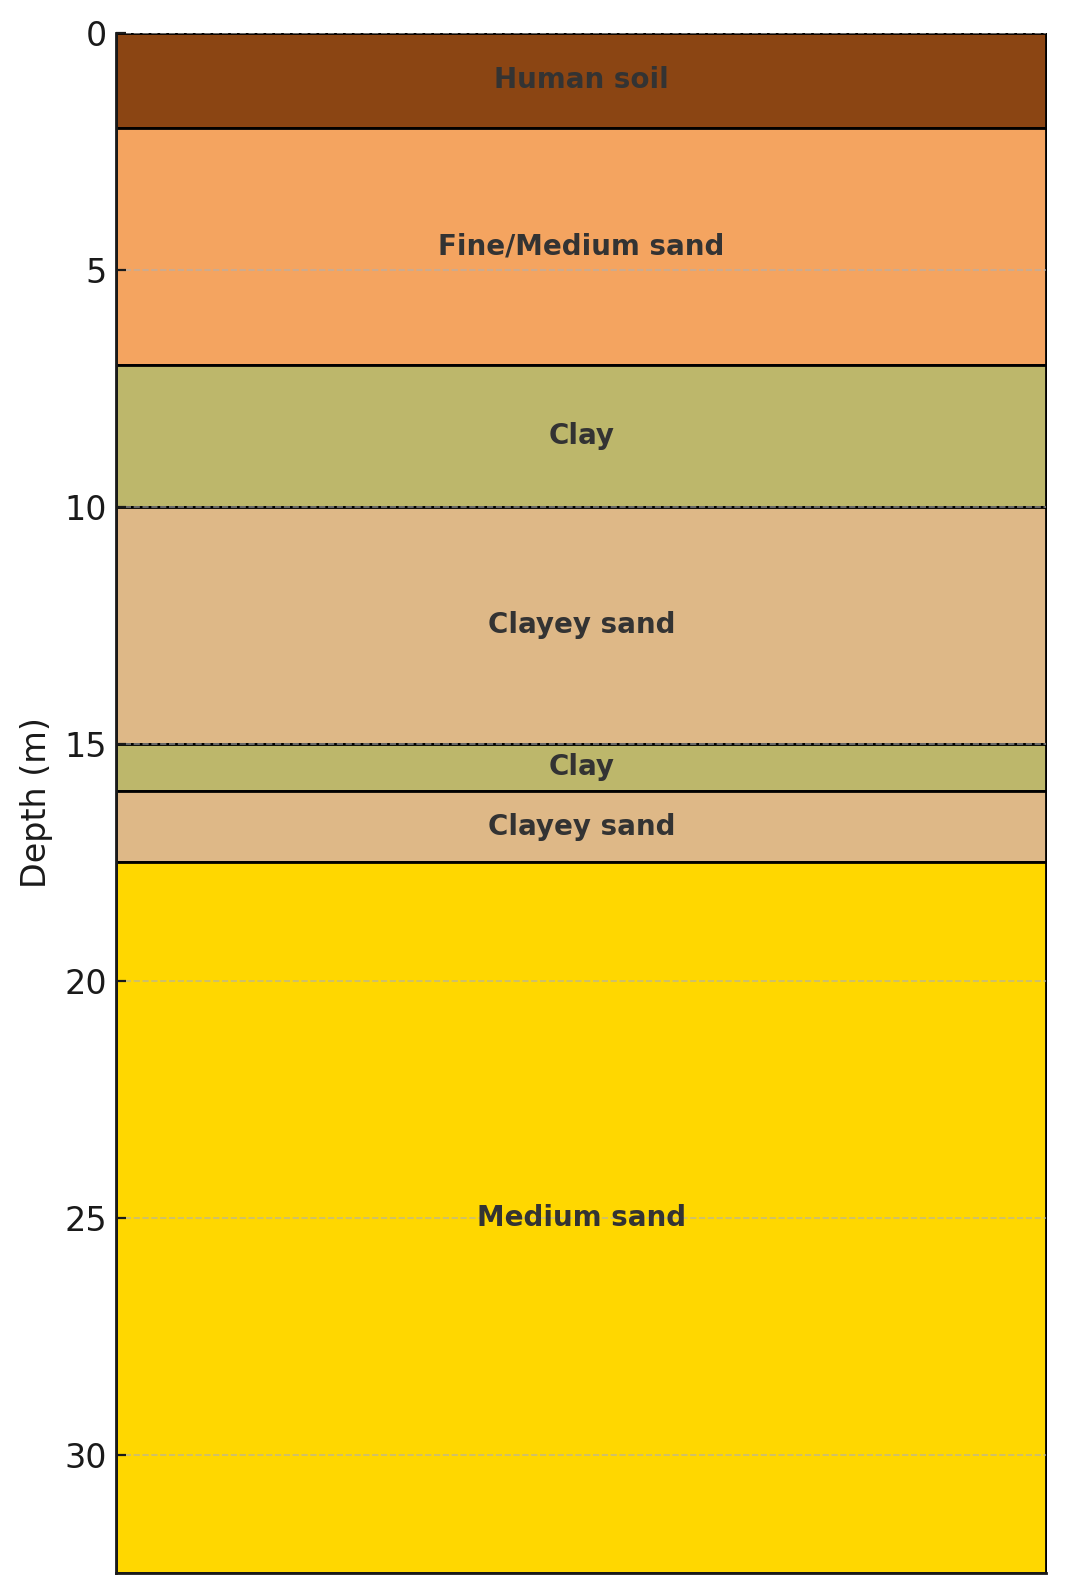
\includegraphics[width=0.45\linewidth]{figures//ch9/Bodemprofiel.png}
    \caption{Borehole profile in Puerto Ibicuy \autocite{amatoEstratigrafiaCuaternariaSubsuelo2009}}
    \label{fig:borehole}
\end{figure}

\subsection{Characteristics of fracking sand}
\label{sec:Charact. of fs}
Sand used in the fracking process must have fairly specific characteristics in order to be usable for fracking. silica sand is mainly used for fracking. This is sand with a grain size between 0.0625 and 2.0 millimeters. The quartz grain content must be higher than 90%. 

Means of transport such as waves and currents in rivers promote the removal of finer or organic particles, thereby ensuring a higher percentage of quartz grains. This is one of the reasons why sand from the Paraná Delta is suitable for fracking.
In addition to erosion by water, the action of wind also influences the characteristics of sand. It causes changes in texture and generally makes quartz sand rounder. 

The specifications for silica sand are written down in the international test standard ISO 13503-2:2006. The important aspects are as follows:

\begin{enumerate}
    \item  Size and distribution of the particles
    \item Shape of the particles
    \item Acid resistance 
    \item Fracture and compressive strength of the grains
    \item Clay and silt content
\end{enumerate}

When it comes to size distributions of the sand particles, the most important is that 90 per cent or more is found in a small size range. Thereby is the size of the particles of less importance and can per badge differ. But when using a sand badge, that badge must have almost exact the same distribution. 

The shape of the sand particles must be round enough and smooth enough to be applicable. Therefore is the system of Krumbrein, W.C. en Sloss, LL. used. This system is shown in Figure \ref{fig:RT}. The norm says that for both roundness as sphericity the value must as least be 0.6. It's important to mention that this procedure is visual and therefore depends on the subjective perception of the person analysing the sample.

\begin{figure}[H]
    \centering
    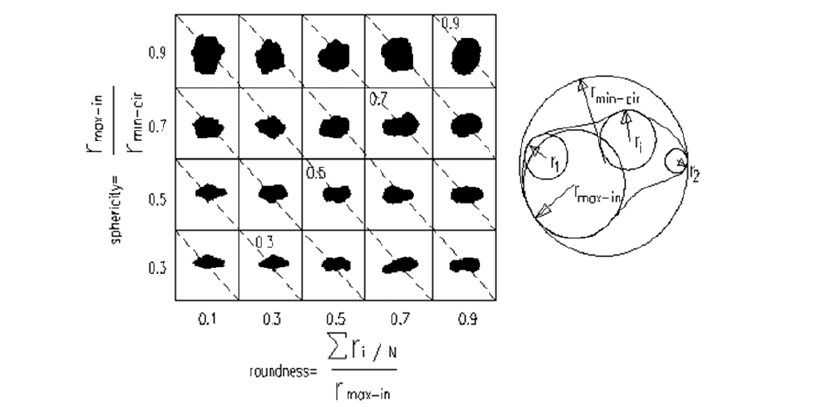
\includegraphics[width=0.75\linewidth]{figures//ch9/roundness.png}
    \caption{Roundness table \autocite{rodriguezParticleShapeQuantities2013}}
    \label{fig:RT}
\end{figure}

Acid solubility testing is used to determine the concentration of soluble elements that contaminate the binder. These elements are typically softer materials that can break down and migrate into the artificially created pore system during fracture closure. This process can lead to conductivity issues within the formation.
To evaluate this are various acids  used of which most are hydrochloric and hydrofluoric acids. These acids dissolve soluble grains such as carbonates, clays, and oxides, while leaving quartz grains intact. Because of this behaviour, industry regulations specify maximum allowable levels of acid-soluble materials that could significantly reduce the permeability of cracks in the wells.
For coarser frac sand with a grain size up to 30/50 mesh, a maximum of 2\% acid-soluble content is permitted. For finer sands, this limit increases to 3\%, as shown in \ref{tab:acid} below.

\begin{table}[h!]
\centering
\begin{tabular}{|c|c|c|}
\hline
\textbf{Particle size (ASTM)} & \textbf{Particle size (mm)} & \textbf{Max. solubility (\% by weight)} \\ \hline
6/12 to 30/50 & 1.68/3.36 to 0.30/0.60 & 2.0 \\ \hline
40/70 to 70/140 & 0.21/0.42 to 0.10/0.21 & 3.0 \\ \hline
\end{tabular}
\caption{Recommended maximum acid solubility \autocite{secretariadepoliticamineraArenasParaFracking2019}}
\label{tab:acid}
\end{table}

For the compressive strength of grains is a test conducted which puts a pressure on the sand particles and then sieves the sample to look which percentage of the particles go trough a certain sieve. This percentage of breaking particles in combination with the known applied pressure tells us which pressure the sand can withstand when using it for making cracks.
The permeability of the fracks in the oil sources drops rapidly if the percentages of cracking sand particles and clay/silt particles is too high. 

\subsubsection{Characteristics of Ibicuy specific}

The sand of the Ibicuy region in the province of the Entre Rios is mostly composed of quarts (86\%). But the sand is quite polluted by iron minerals. The percentage of heavy minerals is very low (0.3\%). This is one of the reasons that the sand is washed before transporting it to the fracking plants \autocite{secretariadepoliticamineraArenasParaFracking2019}. 

\subsection{Consequences of dry sand mining}
The effects of dry sand mining can be diverse. This section combines various reports on dry sand mining as well as knowledge that arises from stakeholder interviews to provide an overview of the consequences that can be linked to this activity.

\subsubsection{Effects on natural habitats}
The most obvious effects due to dry sand mining have to do with the natural environment. As became clear in stakeholder interviews, sand mining leads to the removal of several meters of top soil. This operation requires clearing land of their natural cover: forests or grasslands are removed.

During the interview, the YPF sand mine manager showed two sites where sand mining activities were stopped due to exhaustion of the sand resource. He explained that after mining activities are completed, the areas are left uninterrupted and are thus `given back to nature'. Figure \ref{fig:aftermining} shows the current condition of two former sand mining locations. On the left, activities ceased one year ago and on the right, mining has stopped since four years. The mined areas can be seen in the back of the photos, the sand in the foreground is not part of these sites.

\begin{figure}[H]
    \centering
    \includegraphics[width=1\linewidth]{figures/ch9/Aftermining.png}
    \caption{The state of `finished' locations: after 1 year (left) and after 4 years (right) (Own work)}
    \label{fig:aftermining}
\end{figure}

From figure \ref{fig:aftermining}, it seems that the natural cover (grasslands and forests) has recovered quite quickly in this case. It must however be noted that changes to the original natural environment can still be severe: the original soil profile has drastically changed, meaning that even though a new natural cover has emerged, original species might not be able to survive anymore.

Examples of this can be found in the United States of America: over the past decades, the Dunes Sagebrush Lizard has seen more than 95\% of its original habitat in Texas and New Mexico disappear. This is due to the oil industry and the large scale sand mining operations that support it. In 2024, the species was listed as endangered by the U.S. Fish and Wildlife Service \autocite{centerforbiologicaldiversityLegalInterventionLaunched2025}. Sand mining leads to permanent removal of habitats, which means that letting natural cover grow back may not be enough for species like these to return.

\subsubsection{Social effects}
The most frequently voiced concerns of stakeholders is the poor conditions of roads, especially the provincial RP45 that forms the entrance to the town, caused by intense heavy truck traffic. These comments were confirmed during the field trip, since many potholes were observed along the entire route.

The poor road conditions are not only uncomfortable but also dangerous. In fact, in 2020 alone, ten people lost their lives on the roads that form part of the sand transport routes. The situation has lead to protesting citizens and to blockages of the national highway 12 \autocite{novasImpactoAmbientalOculto2022}.

Other possible negative effects on people living near the sand mines include noise pollution and light pollution, although these concerns were not raised by stakeholders that were interviewed.

\subsubsection{Economic effects}
In the short term, sand mining can contribute to the economic development of an area. Jobs are created and the government can profit through direct and indirect taxation of the activities. However, since all sand mining activities face a natural end (the YPF mine operator indicated that his mine had resources to stay open for 8 more years), positive economic effects do not persists in the long term. A closer look at the situation in Ibicuy reveals more economic troubles related to sand mining.

The Argentinian mining codes dictate that so-called `third-category mines', such as silica sand mines, belong solely to the owner. The government therefore does not receive royalties for exploitation of the areas but instead charges taxes based on volumes \autocite{novasImpactoAmbientalOculto2022}. Instead, the mayor and YPF mine manager indicated that both provincial and municipal taxes are in place. The transport is taxed and each truck pays a tax based on the mass it carries.

From 2019 until 2023, the provincial government of Entre Ríos chose to not adjust the mining taxes, such that the provincial income from these taxes was approximately stable at 400 million pesos per year. However, this period was marked by high inflation and strong devaluation of the Argentine peso \autocite{bellatoEntreRiosFrigerio2025}. In December 2019, at the start of the previous administration's term, 400 million pesos equaled approximately 3 million Euros. At the end of their ruling, in December 2023, the same sum was worth 440.000 Euros, enough for repaving around 1 kilometer of road that is in `fair' condition, by U.S. standards \autocite{crumbCostRoadMaintenance2024}. 

The new provincial government tried to strike a deal with fossil fuel companies to secure investments in infrastructure. After this turned out fruitless, taxes were raised by a factor six in May 2025. As of today, trucks pay 2250 Argentine pesos per ton, a rate that, according to the president of Entre Ríos’ tax authority, still falls short of covering the province’s road repair costs \autocite{crumbCostRoadMaintenance2024}. 

Both the province and municipality charge taxes on transported sand. However, in 2022, municipal mining taxes were only around one tenth of the taxes the province charged on the activity \autocite{novasImpactoAmbientalOculto2022}. At 37 million pesos, the municipal taxes are too low to contribute significantly to road reparations.

\subsubsection{Air quality and health}
During mining, washing and transport processes, silica-rich sands release airborne crystalline silica particles (silica dust). When the silica dust is inhaled, it can contribute to respiratory diseases like silicosis and lung cancer \autocite{physiciansforsocialresponsibilityCompendiumScientificMedical2023}. In 2013, the National Institute for Occupational Safety and Health (NIOSH) tested silica concentrations in 11 sand mining locations in the US. They found that 79\% of samples exceeded the recommended limit, and in some cases the found concentrations even exceeded limits that hold while wearing protection masks \autocite{fogliaSedArena2023}. Effects of silica dusts on nearby communities are a topic of discussion. A 2017 study researched crystalline silica concentrations in homes within 800 m of sand mining activities and concluded that exposure seems unlikely to cause chronic health problems to these communities, because of relatively low concentrations \autocite{petersCommunityAirborneParticulate2017}. However, in January 2021, a ban on frack sand mining in Winona County, Minnesota, US, was upheld by the Supreme Court. The ban was put in place by the county out of concerns about environmental and health impacts \autocite{physiciansforsocialresponsibilityCompendiumScientificMedical2023}.

\subsubsection{Washing operations}
After the sand is mined, it is washed to clean it from unwanted substances such as clay and organic material. For this, large amounts of groundwater are used. In Ibicuy, the sand miners use water from the Talavera formation, which is the same water that flows out of the tap. 

Sand mining companies are reluctant to share information about extracted groundwater volumes. However, in 2020, an environmental information lawsuit revealed 33 documents with specifics. At the time there were 5 sand-washing installations near Ibicuy that together extracted 400 million liters of groundwater per month from the Talavera formation. In comparison, the drinking water cooperation extracts 30 million liters per month in winter and 60 million liters per month in the summer \autocite{fogliaSedArena2023}. Considering the further increase in mining activities since 2020, it seems likely that even more groundwater is extracted now. 

In addition to drinking water competition, the sand washing installations have the capacity to pollute water reservoirs, an effect that is already noticeable in Ibicuy. In june 2022, the local water treatment company reported manganese concentrations of 0.75 mg per liter, whereas the recommended water concentration limit for lifetime exposure is 0.3 mg/L. Further, iron concentrations of 0.93 mg and 1.10 mg were found, an increase of 2200\% as compared to the historic value of 0.05 mg. Additionally, flocculants such as polyacrylamide are used to clump together clay particles and other fine suspended solids. Polyacrylamide can infiltrate into the surface and the underground and can break down into acrylamide during drying \autocite{fogliaSedArena2023}. The WHO warns that acrylamide is genotoxic and carcinogenic, thus may increase the risk of cancer and is therefore a human health concern \autocite{worldhealthorganizationAcrylamide2011}.
\chapter{Hydrodynamical and sedimentary analysis}
\label{chap:hydroanalysis}
\section{Effect of tides and waves on the water level}

\subsection{Tides, waves and currents}
In addition to the study on the effects of sand mining on the river bed, it is as important to look at the effects of water on the river banks.

Relevant to this project, the two situations that contribute to this problem are the elevation of the water level due to the high astronomical tide, and the elevation of the water level/current due to the ship waves.

\subsubsection{Astronomical tides}

Tide is the rise and fall of the water level, in particular the sea level, due to the gravitational force of the moon\autocite{usdepartmentofcommerceTidesCurrents}. As said, the tidal influence is the strongest in the ocean, pulling away the sea from one side of the globe to the other depending on the position of the moon, as seen in Figure \ref{fig:Tidal movement due to gravitational force}.
\begin{figure}[H]
    \centering
    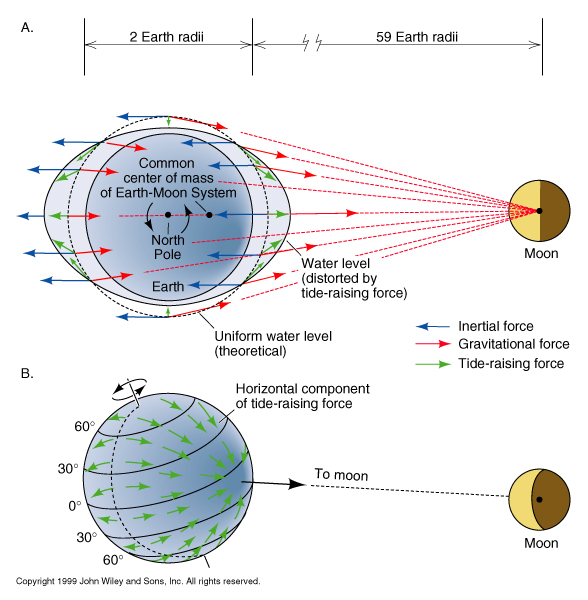
\includegraphics[width=0.5\linewidth]{figures/ch2/astronomical.jpg}
    \caption{Tidal movement due to gravitational force}
    \label{fig:Tidal movement due to gravitational force}
\end{figure}
This gravitational force can also apply to rivers, as long as they are part of, or near a substantial quantity of water mass. Since the region of interest the  Rio Paraná Guazú and Ibicuy are quite near the delta of the Paraná and the river mouth, it is expected to be of significance for the data analysis. This will be treated in section \ref{sec 5.2 Hydrodynamic data}.

\subsubsection{Waves}

The gravitational force not only yields a change in water level, but is also responsible for tidal waves. These are induced by the gravitational pull, in the direction of the moving current. 
In addition to that, there are also wind waves. These are produced by a striking distance called the fetch, where the wind blows on the surface of the water, gathering energy which translates into a wave. In order to find the significant wave height of this situation, one takes a sample of wave heights from buoys and takes the average of the highest third waves \autocite{jaimearrigaSlidesLecture2}.

Given that the river is not straight, the fetch or striking distance is usually quite short, as seen in Figure \ref{Figure 1.1}. This means that the impact of the wind waves is probably quite small. This subject will also be treated in section \ref{sec 5.2 Hydrodynamic data}.

The last part of the waves that will be treated in this subsection are the ship waves. These are created when a ship passes by and pushes away the water to make way for the boat to go forward. This situation initiates three types of waves, primary, secondary, and propeller wash waves, as seen in Figure \ref{Fig:Ship Waves Effect on Water and Bank} below \autocite{Lecture12Ships}.

The impact of the secondary wave is the most promiscuous, as one can tell from the frequency plot underneath the sketch.

\begin{figure}[H]
    \centering
    % First subfigure
    \begin{subfigure}[a]{0.48\linewidth}
        \centering
        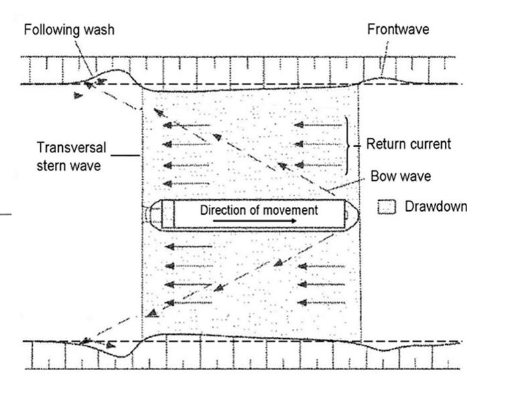
\includegraphics[width=0.5\linewidth]{figures/ch2/shipwaves.png}
        \caption{Ship Waves}
        \label{fig:Ship Waves}
    \end{subfigure}
    
    \vspace{0.5cm}
    
    % Second subfigure
    \begin{subfigure}[b]{0.48\linewidth}
        \centering
        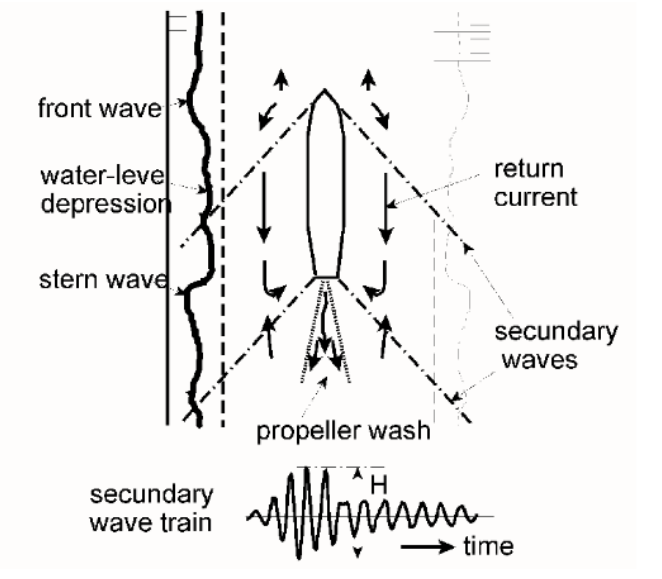
\includegraphics[width=0.5\linewidth]{figures/ch2/shipsecond.png}
        \caption{Propeller Wash Wave}
        \label{fig:Prop Wash Wave}
    \end{subfigure}
    
    \caption{Ship Waves Effect on Water and Bank}
    \label{Fig:Ship Waves Effect on Water and Bank}
\end{figure}


\subsubsection{Correlated currents}

Due to changes in water level as well as supplementary waves, a change in current applies. Using the standard values of the Netherlands and the given facts about the size of the ships circulating and the currents in the Rio Paraná Guazú, one could assume the wave height and current amplitudes for our case. This can be reflected once the field measures are known, in a later section \ref{Section 5}.
The table of the referencing values are as follows:

\begin{table}[H]
    \centering
    \caption{Standard values for wave heights and currents in the Netherlands (Data from CUR 197 ``Breuksteen in de praktijk'').}
    \label{tab:standard_values}
    \begin{tabular}{lcccc}
        \toprule
        \textbf{Location} & \multicolumn{2}{c}{\textbf{Wave heights (m)}} & \multicolumn{2}{c}{\textbf{Currents (m/s)}} \\
        \cmidrule(lr){2-3} \cmidrule(l){4-5}
        & \textbf{Wind waves} & \textbf{Ship waves} & \textbf{Natural current} & \textbf{Return current} \\
        \midrule
        Lakes          & 0.25 -- 1.00  & 0.10 -- 0.50  & 0.1 -- 0.5  & 0.1 -- 0.25 \\
        Canals         & 0.10 -- 0.25  & 0.25 -- 0.75  & 0.5 -- 1.0  & 0.5 -- 1.0  \\
        Rivers         & 0.25 -- 1.00  & 0.25 -- 0.75  & 1.0 -- 2.0  & 0.5 -- 1.0  \\
        Small waters   & 0.10 -- 0.20  & n.a.          & 0.2 -- 1.0  & n.a.       \\
        \bottomrule
    \end{tabular}
\end{table}


Understandably, the relevant row for this project is the 'River' category. Hinting to the fact that big ships are usually present in the channel, one might take values towards the upper boundary of the table.

\subsection{Loads and Impacts due to Ships}
Following the information about tides, waves and currents one might ask what type of forces these contain and what how the loads could be quantified. This can be done with the help of wave theory. 

The first relevant parameters to take into account are the ship waves in rivers. These are assumed to be between 0.25 and 0.75 meters tall. Based on observations during the field trip, the value of 0.25 meter wave height is chosen as the cargo's do not travel with a speed significant enough to reach a height of 0.75 m \ref{tab:standard_values}. 
In addition to that, the current coming from the ship, both natural and return are also relevant. Since the Natural current is relevant in this case, the value of 1.5 [m/s] will serve as a reference for further calculations.
This gives the following parameters:

\begin{table}[H]
    \centering
    \caption{Parameters for Wave Impact Calculation}
    \label{tab:Parameters for Wave Impact Calculation}
    \begin{tabular}{lcc}
        \toprule
        \textbf{Location} & \textbf{Ship wave height: H (m)} & \textbf{Natural current: u (m/s)} \\
        \midrule
        Rivers & 0.25 & 1.5 \\
        \bottomrule
    \end{tabular}
\end{table}

\subsubsection{Wave Load}
Next, one can calculate the force of the wave, assuming that the wave signal given by the boat is uniform, and at about 10 repetitions 100 meters from the shore
This leaves us with the theory of waves \autocite{} which states that there are two types of waves you can get energy from:
There are two types of waves for which we can calculate energy.

\begin{itemize}
    \item periodic waves 
    \item random waves 
\end{itemize}

Wave energy is a specific energy and it's calculated per unit of horizontal area [J/m$^2$].

The formula (equation) to calculate wave power is:

$$
{E_{pw} = \left(\frac{1}{8}\right) \cdot \rho \cdot g \cdot H_{m0}^2}
$$

$$
{E_{rw} = \left(\frac{1}{16}\right) \cdot \rho \cdot g \cdot H_{m0}^2}
$$

\noindent where:
\begin{itemize}
    \item $\rho$ : is the density of fresh water: 1000 [kg/m\textsuperscript{3}];
    \item \(\mathbf{v}\) is the flow velocity vector, expressed in meters per second [m/s];
    \item \(H_m0\) is the wave height: 0.50 [m];
    \item \(g\) is the gravitational constant: 9.81 [m/s\textsuperscript{2}]
\end{itemize}

From the situation we have, on a small interval of time, the ship waves can be assumed to be periodic. Therefore the first version of the formula can be used. 

Filling the parameters in the equation yields: 

$$
E_{pw} = \frac{1}{8} \cdot 1000 \cdot 9.81 \cdot (0.25)^2 = 76.64 \, \text{J/m}^2
$$

Converting units gives:
$$
{F_w}= 0.7664 \, \text{[kN/m]}
$$
For every wave coming from the boat, this load has to be summed times 10. This has to be applied every time a boat passes by.

Based on the fact that there are 6 boats a day that pass, one might assume $ E_{pw} = 45.98  \, \text{kN/m}$ per day. 

\subsubsection{Current Load}
For the current load, one might use the drag equation\ref{offshore}
because it can be used to calculate the force exerted by a current on a vertical structure:

$$
F_c = \frac{1}{2} \rho C_d A u^2
$$

\noindent where:
\begin{itemize}
    \item \textbf{$ F_c $}: Force exerted by the current [N]
    \item \textbf{$ \rho $}: Density of freshwater: 1000 [kg/m$^3$]
    \item \textbf{$ C_d $}: Drag coefficient, for a vertical wall: 1.2 [-]
    \item \textbf{$ A $}: Exposed area:  [m$^2$]
    \item \textbf{$ u $}: Current velocity: 1.5 [m/s]
\end{itemize}

To be able to calculate the force of the current on the bank, one needs to establish the exposed area [m$^2$]. Since we do not know exactly how long the bank is we could calculate with A = 1 [m$^2$] to find a Force illustrated per meter length of the bank.

Filling in these parameters gives:

$$
F_c = \frac{1}{2} 1000*1.2* 1.5^2 = 1.350 \text{[kN/m]}
$$
This also occurs for a short period of time, but 6 times a day.

Hence, the total load effect of the ship waves on the bank would be:

$$
F = F_w + F_c = 1.350*6 + 45.98 = 54.08 \text{[kN/m]}
$$

This value can later be used when calculating solutions for bank protection. 

\subsection{Effect on the river bed}
\label{chap 6: effect on the river bed}
There are several ways how the water could have a negative impact on the river bank. In theory the river bank failure may be caused by house placement, water saturation, weight on the river bank, vegetation, and/or tectonic activity, but most of them due to the rise of the water level. The reason behind this is that the river bank is naturally eroded when the water exerts a force on it.
The river bank is divided in three parts: the toe, the bank and the overbank zone. The toe of the bank is the most susceptible to erosion when in contact with high water levels, which can be seen in the Figure \ref{fig:Effect of Water on Bank after One Year} below \autocite{australiaRiverbankCollapse}.

\begin{figure}[H]
    \centering
    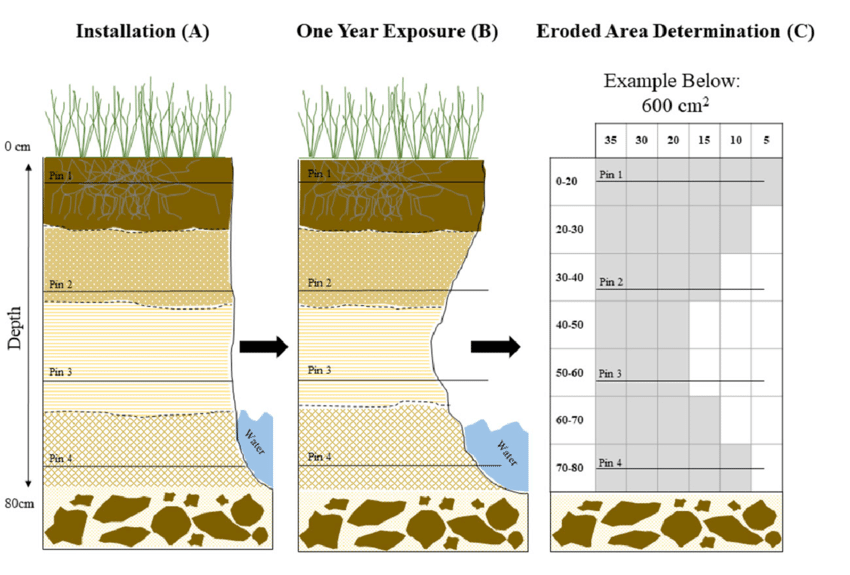
\includegraphics[width=0.5\linewidth]{figures/ch2/Erosion.png}
    \caption{Effect of Water on Bank after One Year}
    \label{fig:Effect of Water on Bank after One Year}
\end{figure}

When the combination of water level with a strong current is highest, the bank zone is affected by the tidal currents or waves. This is because, as seen in the Figure 7.2, water erodes the layer of the bank where the extra water level pushes, creating a dent inside the soil layer.
Consequently, after some time the upper overbank area has less and less support underneath, becoming thus unstable and partly falling down. 
Repeating this process takes the river bank further inside the land, increasing the channel width, absorbing the land of the local communities or agricultural fields that live near the river bank.


\section{Hydrodynamic data}
\label{sec:Hydrodynamic data}
In this section, analysis on the hydrodynamic variables is performed. This includes relations between water elevations, discharge and sediment concentrations - both through data sources and field measurements. Additionally, tidal effects in the study area are considered. 

\subsection{Conversion to water elevation}
A uniform approach is needed to describe water levels and depths of the river. Therefore, these variables will be expressed in terms of a reference level, IGN, which is set by the \textit{Instituto Geográfico Nacional}. It is based on sea level measurements from a tide gauge in Mar del Plata, Buenos Aires province (\cite{ReferenciaVerticalInstituto}). Figure \ref{fig:waterelevationreference} gives an overview of the quantities with respect to an arbitrary measurement station. Here, $d$ is the vertical depth as measured by the ADCP or echosounder. Moreover, each station has a specific distance between its local zero reference and the zero IGN level, which is indicated by $l_{station-IGN}$. Next, all variables should be expressed in terms of IGN level. Therefore, water elevations and depths expressed in elevation are defined as follows:

\begin{equation}
    we_{station} = wl_{station} + l_{station-IGN} ~[m~IGN]
\end{equation}

\begin{equation}
    d_{el} = we_{station}-d ~[m~IGN]
\end{equation}


\begin{figure}[H]
    \centering
    \includegraphics[width=0.75\linewidth]{figures/ch5/waterelevations.png}
    \caption{Water elevation reference}
    \label{fig:waterelevationreference}
\end{figure}

\subsection{Flow partitioning}

At some point in the Lower Paraná, the river splits into two main tributaries, as shown in Figure \ref{fig:flow partition}. To have an approximation for the distribution of discharge between these rivers, the discharge series are given in Figure \ref{fig:discharge_series}. From these plots, it follows that the majority of the discharge flows into the Paraná Guazú. Figure \ref{fig:flow_partition} represents this ratio and plots a linear fit. As there is no significant increase or decrease, the approximation is made that 78\% of the total discharge upstream of the confluence flows into Paraná Guazú. \citeauthor{reMETODOLOGIAPARAGENERACION2009} report that a linearly increasing trend occurs. In this study, more data points are used and therefore the approximation of a constant percentage is assumed sufficient. 

\begin{figure}[h!]
    \centering
    % First subfigure
    \begin{subfigure}[b]{0.48\linewidth}
        \centering
        \includegraphics[width=\linewidth]{figures/ch5/discharge series.png}
        \caption{Discharge series obtained from Brazo Largo and Zárate measurement stations}
        \label{fig:discharge_series}
    \end{subfigure}
    \hfill
    % Second subfigure
    \begin{subfigure}[b]{0.48\linewidth}
        \centering
        \includegraphics[width=\linewidth]{figures/ch5/flow partition.png}
        \caption{Flow partition, expressed as the share of total flow that streams into Paraná Guazú}
        \label{fig:flow_partition}
    \end{subfigure}
    
    \caption{Comparison of discharge divided between Paraná Guazú and Paraná de las Palmas}
\end{figure}



\subsection{Water elevations and discharge}
This section describes the discharge observed in the measurement stations and relates it to water elevation data. Traditionally, stage-discharge relations are described by rating curves that describe power-law dependencies between variables. This can be written in the following form, with $Q$ the discharge and $h$ the water level or stage:

\begin{equation}
\label{eq:powerlaw}
    Q = a \cdot h^b
\end{equation}

In the expression above, $a$ is a constant and $b$ an index exponent. \citeauthor{schmidtStageDischargeRelationshipOpen2011} note several limitations related to these rating curves. For example, discharge measurements typically scatter and therefore do not show a unique relation with the stage. Also, the underlying physics of the open channel are not captured in the rating. Nevertheless, the relation as given in Equation \ref{eq:powerlaw} is used to roughly approximate dependencies between the variables. 

The relationship between fluvial discharge and water level at Brazo Largo yields a relatively weak correlation with an $R^2$ of 0.365. This is shown in Figure \ref{fig:waterleveldischarge}. Alternatively, a linear fit was assumed which produced a slightly better result, showing a positive trend with an $R^2$ of 0.444. In contrast, the El Colorado and Túnel Subfluvial stations exhibit a clear power-law dependence. Power-law fits for these stations resulted in higher $R^2$-values of 0.962 and 0.712, respectively, with the El Colorado plot shown in Figure \ref{fig:waterleveldischarge}. Overall, these results suggest that the strength of the water level–discharge relationship decreases as the river flows downstream.


\begin{figure}[h!]
    \centering

    \begin{subfigure}[t]{0.48\linewidth}
        \centering
        \includegraphics[width=\linewidth]{figures/ch5/wl discharge Brazo Largo.png}
        \caption{Stage–discharge relation in Brazo Largo.}
        \label{fig:wl_discharge_brazo}
    \end{subfigure}
    \hfill
    \begin{subfigure}[t]{0.48\linewidth}
        \centering
        \includegraphics[width=\linewidth]{figures/ch5/wl discharge El Colorado.png}
        \caption{Stage–discharge relation in El Colorado.}
        \label{fig:wl_discharge_colorado}
    \end{subfigure}

    \caption{Water elevation–discharge relationships for two measurement stations.}
    \label{fig:waterleveldischarge}
\end{figure}



\subsection{Sediment loads}
When extending the analysis to the sediment concentrations, the same trend occurs: in the Bermejo river, fine and course sediment discharges are closely related to large flow events through power-law relations. This behaviour is found to a lesser extent in the lower Paraná, where the correlations are relatively weak. Figure \ref{fig:discharge sediment brazo} shows this relation between sediment concentrations and river discharge for the Brazo Largo station. Overall, a power-law fit seems a good approach to model the relation. The fine sediment concentration is generally higher than the course sediment concentration. In addition, the course sediment concentration increases more significantly for an increasing fluvial discharge. These are general trends, but it has to be stressed that the $R^2$ of both relationships is relatively low. As a comparison, the same variables are related for the Bermejo river in Figure \ref{fig:discharge sediment bermejo}. 


\begin{figure}[h!]
    \centering
    % First subfigure
    \begin{subfigure}[b]{0.48\linewidth}
        \centering
        \includegraphics[width=\linewidth]{figures/ch5/discharge sediment brazo largo.png}
        \caption{Fine and course sediment loads in relation to discharge at Brazo Largo}
        \label{fig:discharge sediment brazo}
    \end{subfigure}
    \hfill
    % Second subfigure
    \begin{subfigure}[b]{0.48\linewidth}
        \centering
        \includegraphics[width=\linewidth]{figures/ch5/discharge sediment bermejo.png}
        \caption{Fine and course sediment concentrations in relation to discharge at Bermejo}
        \label{fig:discharge sediment bermejo}
    \end{subfigure}
    
    \caption{Fine and course sediment loads related to fluvial discharge in two measurement station}
    \label{fig:sediment loads and discharge}
\end{figure}

\subsection{Correlation between variables}
The approach of defining the relations between measured flow variables is as follows. First, the values in the dataset are log-transformed, after which $R^2$-values are calculated based on a linear fit on the logarithmic values. This procedure is applied to the variables of all measurement stations as described in Section \ref{sec:measurementstations}. Figure \ref{fig:correlationmatrices} gives the results for El Colorado and Brazo Largo in the form of correlation matrices. It stands out that correlations in the Bermejo are very high for all variables. This indicates that the power-law assumption is suitable for describing the dependencies between these variables. Subsequently, it is found that correlations for the Brazo Largo are much smaller. This is also the case for the Zárate station on the Paraná de las Palmas. As this river is also located in the Lower Paraná, this behaviour is expected. 

Analysis of the flow variables has shown that $R^2$-values tend to decrease, the further downstream the location of the measurements is. This result is in agreement with those found by \citeauthor{songEvaluatingUnderstandingTideriver2024}, who state that the stage-discharge relationship is considerably affected in the transitional zone and tide-dominated region of the Yangtze estuary. Their research reports $R^2$-values decreasing from 0.9 to 0.4, in a river-dominated and transitional zone, respectively. Therefore, an in-depth study of the tide-river interactions is needed. This includes measurements in both the transitional zone and tide-dominated region, to update the stage-discharge relationship. For this particular study, the influence of tidal effects will be handled in Section \ref{sec:tidal forcing}.

As for the sediment-discharge relationship, the differences in correlations in Brazo Largo can be explained through the sources of the variables. Whereas the fine sediment concentration predominantly originates from the Bermejo basin, the discharge is dominated by the Paraguay and Paraná. This results in a weak correlation downstream of the confluence of these rivers (\cite{lopezweibelSourcesTemporalDynamics2022}). Another factor that may perturb the correlation of variables in the Lower Paraná, is the inflow of the Uruguay river. This flow can cause disturbances in the relations, as the sediment concentrations and discharges stem from different catchments. 





\begin{figure}[h!]
    \centering
    % First subfigure
    \begin{subfigure}[b]{0.48\linewidth}
        \centering        \includegraphics[width=\linewidth]{figures/ch5/logcorrelations Brazo Largo.png}
        \caption{Correlation matrix of log-transformed data in Brazo Largo}
        \label{fig:logcorrelation brazo}
    \end{subfigure}
    \hfill
    % Second subfigure
    \begin{subfigure}[b]{0.48\linewidth}
        \centering
        \includegraphics[width=\linewidth]{figures/ch5/logcorrelations Bermejo.png}
        \caption{Correlation matrix of log-transformed data in El Colorado}
        \label{fig:logcorrelation bermejo}
    \end{subfigure}
    
    \caption{Comparison of $R^2$-values at Brazo Largo and El Colorado}
    \label{fig:correlationmatrices}
\end{figure}




\subsection{Tidal forcing}
\label{sec:tidal forcing}
The tidal wave of the Atlantic Ocean influences the hydrodynamics of the lower Paraná delta. As the tidal wave enters the delta ta Río de la Plata, the tide is damped and phased by friction, channel geometry and branching, resulting in a reduced amplitude and an increased in phase delay. Under normal conditions, the influence of the tide on the Paraná River reaches the city of Villa Constitución, which is located 220 km upstream of the river mouth. For storm conditions, the tide can reach the city of Rosario \autocite{balayCAUSESPERIODICITYLARGE1958}. In order to determine the influence of the tide at Brazo Largo, a reference water level at San Fernando is considered. It is assumed that at San Fernando no tidal damping has occurred, therefore the tidal amplitude at Brazo Largo can be determined using the following relation:

\begin{equation}
    A_{\text{Location}} = \alpha \cdot A_{\text{SanFernando}}
\end{equation}

The damping coefficient ($\alpha$) and the tidal delay with respect to San Fernando have been determined by Brok (2022). For Brazo Largo, a damping coefficient of 0.3 and tidal delay of 4 hours were found. These values will be used as reference values when isolating the tide at Brazo Largo. The tidal signal is isolated using hourly water level data for a period of more than 2 years from both Brazo Largo and San Fernando. Table 5.2 shows the tidal constituents  considered and their period.

\begin{table}[h!]
\centering
\caption{Tidal constituents used to reconstruct the tide
\autocite{BRON}.}
\label{tab:constituents}
\begin{tabular}{lccc}
\hline
\textbf{Tidal constituent} & \textbf{Name} & \textbf{Period [h]} \\
\hline
\multicolumn{3}{l}{\textit{Semi-diurnal}} \\
\hspace{1em}Principal lunar & M2 & 12.4206\\
\hspace{1em}Principal solar & S2 & 12.0000 \\
\hspace{1em}Lunar elliptical & N2 & 12.6583\\
\hline
\multicolumn{3}{l}{\textit{Diurnal}} \\
\hspace{1em}Lunar-solar declinational & K1 & 23.9345  \\
\hspace{1em}Principal lunar & O1 & 25.8193  \\
\hline
\multicolumn{3}{l}{\textit{Shallow water constituents}} \\
\hspace{1em}Overtide of M2 (quarter-diurnal) & M4 & 6.2103  \\
\hline
\end{tabular}
\end{table}

- uitleg hoe het getijde bepaald is

The tidal amplitude and phase of each constituent for San Fernando and Brazo Largo are displayed in Table 5.3. Additionally, the damping coefficient ($\alpha$) and the tide delay are calculated for the different constituents and shown in Table 5.3. The calculated amplitudes show that the delta has mixed tidal dynamics  (semidiurnal-diurnal)
dominated by the semi-diurnal M2 constituent with contributions from N2, K1 and O1. The overtide M4 plays a minor role. The damping coefficient is consistent across the constituents ranging from 0.23 to 0.33, inditcating that the use of formula 5.3 is valid. The calculated time delay of 4.5 - 5.5 hours is also in line with the time delay calculated by Brok (2022). The damping coefficient of M4 is different because it is generated locally with nonlinear interactions.

\begin{table}[h!]
\centering
\caption{Amplitude and phase comparison}
\begin{tabular}{lcccccc}
\hline
Constituent & $A_{\text{SF}}$ & $A_{\text{BL}}$ & $\alpha$ & tide delay [hr] & $\phi_{\text{SF}}$ [$^\circ$] & $\phi_{\text{BL}}$ [$^\circ$] \\
\hline
M2 & 0.253 & 0.058 & 0.230 & 4.450 & -0.465 & 1.786 \\
S2 & 0.041 & 0.010 & 0.239 & 5.055 & -2.526 & 0.121 \\
N2 & 0.094 & 0.022 & 0.238 & 4.316 & -0.546 & 1.596 \\
K1 & 0.119 & 0.037 & 0.313 & 5.181 & -2.543 & -1.183 \\
O1 & 0.187 & 0.061 & 0.328 & 5.517 & 2.694 & -2.247 \\
M4 & 0.030 & 0.006 & 0.189 & -1.495 & -2.608 & 2.162 \\
\hline
\end{tabular}
\end{table}

Figure 5.7 shows the water level time series for a period of 7 days compared to the calculated tidal signal at Brazo Largo. From this figure, it can be seen that the measured water level follows the same tidal oscillations. However, the tide does not explain all the variability of the water level; the measured water level also shows large variability caused by discharge and wind. 
\\The influence of the strong non-tidal component is confirmed by Figure 5.8, which shows the water level at Brazo Largo for a period of 2 years. The measured water level fluctuates greatly, reaching +2.0 m and -0.5 m while the tidal component is steady at 0.0 m with an amplitude of 0.17 m. The tidal forcing is relatively small compared to the river and seasonal influences. Tidal forcing is therefore subordinate to other forcings such as discharge.

\begin{figure}[H]
    \centering
    \includegraphics[width=1\linewidth]{figures/ch5/Tide_Brazo_largo.png}
    \caption{Calculated tide at Brazo Largo for a period of 7 days.}
    \label{fig:period 7}
\end{figure}
\begin{figure}[H]
    \centering
    \includegraphics[width=1\linewidth]{figures/ch5/Tide_BL_2y.png}
    \caption{Calculated tide at Brazo Largo for a period of 2 years.}
    \label{fig:period 2}
\end{figure}

- Waterlevel at Brazo Largo
    (misschien het getijde meenemen?)
\\ - Getijde rond Brazo Largo is berekend aan de hand van waterlevel rond San Fernando. Vergelijk de constituents met die van  het rapport en trek conclusie over invloed getijde.



\section{Sediment transport}




- Bepaal fine sediment-discharge relation bij El Colorado. Reken hiermee door voor het fine sediment concentration bij Brazo Largo

- Bepaal fine sediment concentration op basis van de suspended sediment samples.

- Coarse sediment concentration wordt bepaald met de Engelund-Hansen formule

- Vergelijk dit met de bedload metingen van het veldwerk

- Set up a sediment balance for the area of interest.


- Sediment transport caused by tidal assymetry.


\section{Field work measurements}
This section describes the results of the field campaign introduced in Section \ref{sec:field study}. The measurements are compared to the results found in Section \ref{sec:Hydrodynamic data}.


\subsection{Water level and discharge}
In order to further study the liquid flows in the Paraná Guazú, it is noted that estimates for the discharge of Río Ibicuy and Río Talabera are needed. These were collected during the fieldwork, as indicated in Figure \ref{fig:measurements day1} and Figure \ref{fig:measurements day2}. In addition, an overview of all cross sections with water level and discharge measurements is given in Figure \ref{fig:cross section domain}. The indexing of the cross sections is made in chronological order based on the fieldwork. Note that at the confluence of the Ibicuy and Paraná, there is no measurement of the component flowing in from the Paraná. However, this can be estimated by the equilibrium of discharges in the confluence. The relevant flow measurements of the different cross sections are summarized in Table \ref{tab:discharges fieldwork}. Note that the water levels are recorded at Brazo Largo and Ibicuy, depending on the location and time of each measurement. For Section 5, the water level is linearly interpolated between the stations. Also, the velocity and discharge values are mean values. The bathymetries and velocity profiles that result from the ACDP measurements can be found in Appendix \ref{appendix:fieldwork results}, where the output of the \textit{RiverSurveyor} software is given. Note that of each cross section, only one of the two measured sections is given. 

\begin{table}[H]
    \centering
    \renewcommand{\arraystretch}{1.2} % extra row spacing
    \setlength{\tabcolsep}{8pt}       % extra column spacing
    \begin{tabular}{llccc}
        \toprule
        \textbf{Section} & \textbf{River} & \textbf{Water level [m IGN]} & \textbf{Flow velocity [m/s]} & \textbf{Discharge [$m^3$/s]} \\
        \midrule
        1 & Talabera       & 1.09 & 0.423 & 4402 \\
        2 & Paraná Guazú   & 1.12 & 0.111 & 6562 \\
        3 & Paraná Guazú   & 1.10 & 0.110 & 10748 \\
        4 & Ibicuy & 0.87 & 0.127 & 2901 \\
        5 & Paraná Guazú   & 0.82 & 0.245 & 6758 \\
        \bottomrule
    \end{tabular}
    \caption{Flow properties of fieldwork measurements in different sections}
    \label{tab:discharges fieldwork}
\end{table}


\begin{figure}[H]
    \centering
    \includegraphics[width=0.75\linewidth]{figures/ch5/balance domain.png}
    \caption{Overview of cross sections with discharge measurements}
    \label{fig:cross section domain}
\end{figure}


\subsection{Suspended sediment load}
In this section, the measured suspended sediment concentrations and the measured flow velocity profiles will be analysed in order to calculate the total suspended sediment flux. Section 3.2.2 describes the 

\subsection{Grain size distribution of bed load samples}
During the fieldwork, data was collected on the Paraná River over a period of two days. Seven samples were collected from the riverbed at four different cross-sections. Samples were collected at depths of 10 and 15 metres. The first number refers to the cross-section and the second number refers to a depth of 10 or 15 metres. The locations where the samples were collected are presented in figure \ref{fig:measurements day1} and \ref{fig:measurements day2}. Sample 3-1 was quite large, so it was decided to treat it as two different samples (3-1A \& B). 

When processing the samples, it was decided to start with a 0.5 mm sieve size for the samples that appeared to be sand and a 0.354 mm sieve size for the other samples. This was done because only six sieves and one residue container fit into the sieving setup. After sieving the samples for 10 minutes, each quantity of sample per sieve was weighed. This was used to calculate a cumulative grain distribution. The calculation and processing of the results are in more detailed described in Appendix \ref{appendix:Lab data}. The results are presented in figure \ref{fig:Cumu}.

\begin{figure}[H]
    \centering
    \includegraphics[width=0.75\linewidth]{figures//ch6/cumulativegrainsized.png}
    \caption{Cumulative grain size distribution}
    \label{fig:Cumu}
\end{figure}

Figure \ref{fig:Cumu} clearly shows that 1-2 and 2-2 are sand samples and the other samples are clay and silt samples. During the test there is also looked at possible organic materials. When seeing something that could be organic, the sample was tested with hydrochloric acid to see if this was the case. It was never the case that there were organic particles.

From figure \ref{fig:Cumu} can be seen that the change of finding sand is much bigger on 15 meters depth than on 10 meters depth. This could indicate that the deeper the riverbed is, the higher the change is of finding sand. 

\section{Sediment Balance}

\section{Hydrodynamic effects on the River Banks}
\subsection{Aqua Monitor}
In this section the data from the water gains and losses is explained in more detail.
Recalling the whole period of time available \ref{Aqua Monitor Water Changes 1985-2025}, it is clear that the outer side of the river curves experience a water gain (indicated in blue), and the inside sides of the curves lose water (indicated in green). 
The location of the camping 'La Blanqueada' is in the outer side of the curve near Puerto Constanza, as seen in the following Figure \ref{fig:Camping Blanqueada}.

\begin{figure}
    \centering
    \includegraphics[width=0.5\linewidth]{figures/ch5/Camping Blanqueada.png}
    \caption{Location of the Camping La Blanqueada}
    \label{fig:Camping Blanqueada}
\end{figure}

The camping's location matches with the blue part of the water gain map, indicating that the water quantity around the shore of the camping has increased. 
In order to know if this has always been so, or if the water gains in this precise location have been gradually increasing, several maps with closer intervals have been created. 

There are quite a few comments to be made about the maps. 

First of all, blue and green zones stay consistent throughout the years, but when going into detailed time periods they can differ.

There can be variations in shorter time periods such as the period 2005-2015 which indicated more water gains than losses in the deltas surrounding the region of interest.

Another very interesting thing to note is that the flood of 2016 in the Parana Guazu can also be seen through the help of this map, on a time interval of 2015-2017.

Furthermore, droughts are also illustrated quite well with this software. The perfect example would be the long period of drought in 2022 which led some parts of the Parana to be left for dry, as seen in Figure \ref{fig:Discharge Changes in Brazo Largo}. With the Parana Guazu's significant depths of over 40 meters this was unlikely to happen but still, this change in water quantity did not go unnoticed by the Deltares software. This can be seen on the Figure of 2020-2022.

Other periods of time are more or less stable and have nothing to report.

\begin{figure}[H]
    \centering
    \begin{subfigure}[a]{0.6\textwidth}
        \includegraphics[width=\linewidth, height=5cm]{figures/ch5/2005-2015.jpg}
        \caption{Period 2005-2015}
        \label{fig:Period 2005-2015}
    \end{subfigure}
\end{figure}

\begin{figure}[H]
    \centering
    \begin{subfigure}[b]{0.6\textwidth}
        \includegraphics[width=\linewidth, height=5cm]{figures/ch5/2015-2017.jpg}
        \caption{Period 2015-2017}
        \label{fig:Period 2015-2017}
    \end{subfigure}
\end{figure}

\begin{figure}[H]
    \centering
    \begin{subfigure}[c]{0.6\textwidth}
        \includegraphics[width=\linewidth, height=5cm]{figures/ch5/2020-2022.jpg}
        \caption{Period 2020-2022}
        \label{fig:Period 2020-2022}
    \end{subfigure}
    
    \caption{Water Changes in Different Periods}
    \label{fig:Water Changes}
\end{figure}

\begin{figure}[H]
    \centering
    \begin{subfigure}{0.48\textwidth}
        \includegraphics[width=\linewidth]{figures/ch5/dischargepeak.jpg}
    \end{subfigure}
    
    \caption{Discharge Changes in Brazo Largo}
    \label{fig:Discharge Changes in Brazo Largo}
\end{figure}


For the sake of these explanations the relevant Figures can be found in the Appendix \ref{Appendix: Satellite Data}.

\subsection{Surface Area Measurements}
From the Aqua Monitor Software, one could establish which regions were of interest in a broad scope surrounding the Parana Guazu turn near Puerto Constanza. 

Decreasing the scope leaves us with question marks regarding the actual areas and lengths of land that have been subject to these water gains. Therefore, it was chosen to investigate further into the details of the coast erosion with Google Earth.
Using the software's satellite data, one could draw a surface around the area of the Camping La Blanqueada in 2022, the most recent available, and then compare it to historical data. 
This gives a dataset of historical data from 1985 until 2022 but since the satellite images have been improving with the time, the only relevant data can be taken from 2003 on.


Thus, it was chosen to take the difference in surface area from 2022 until 2003. Initially only the East side of the Camping was taken into account due to its matching with the drone pictures taken of the area during the field trip \ref{fig:Bank Erosion shots from field work}. Nevertheless on Google Earth it quickly became obvious that the necessity rose to take the West part of the Camping in consideration as well since its surface was eroded even further.

A summary of the data gathered from this study can be found below. First the Measurement of the East part of the Camping, then the comparison with 2003, 2017, 2018 and then for both sides the added surface lost since 2003.

\begin{figure}[H]
    \centering
    \begin{subfigure}[b]{0.45\textwidth} % Adjusted width to fit both images side by side
        \includegraphics[width=\linewidth, height=5cm]{figures/appendix-g/opp2022.png}
        \caption{Surface Data for 2022}
        \label{fig:surface2022.2}
    \end{subfigure}
    \hfill
    \begin{subfigure}[b]{0.45\textwidth} % Adjusted width to fit both images side by side
        \includegraphics[width=\linewidth, height=5cm]{figures/appendix-g/opp2017.png}
        \caption{Surface Data for 2017}
        \label{fig:surface2017}
    \end{subfigure}
    \hfill
    \begin{subfigure}[b]{0.45\textwidth} % Adjusted width to fit both images side by side
        \includegraphics[width=\linewidth, height=5cm]{figures/appendix-g/opp2018.png}
        \caption{Surface Data for 2018}
        \label{fig:surface2018}
    \end{subfigure}
    \hfill
    \begin{subfigure}[b]{0.45\textwidth} % Adjusted width to fit both images side by side
        \includegraphics[width=\linewidth, height=5cm]{figures/appendix-g/verlorenopp2003.png}
        \caption{Surface Data for 2003}
        \label{fig:surface2003.2}
    \end{subfigure}
    \caption{Comparison of Surface Data}
    \label{fig:surface_comparison}
\end{figure}

It is known that there was a flood in 2016 \autocite{ArgentinaInundacionesDesde2016}. This flood was in return responsible for a significant increase of water quantity and discharge throughout the region, as seen in Figure \ref{fig:Discharge Changes in Brazo Largo}.

Consequently this affected certain areas of the channel more than others, in particular the curves of the Parana Guazu such as Puerto Guazu showed in the Figures \ref{fig:Water Changes} as discussed before. The negative impacts were highlighted when the high discharge and water quantities dropped back to normal, leaving a part of the bank fragile which then contributed to an accelerated bank erosion.



This argument can once again be solidified by the drastic increase of erosion in between those time periods. After this flood event, the rate of erosion decreased again.

Lastly, both sides of the Camping and the difference between 2003 and 2022 can be seen below. The leftover piece of land which was present in 2003 but has been eroded since then is also traced as a surface area in a distinct colour \ref{fig:surfacelost_comparison}. 

\begin{figure}[H]
    \centering
    \begin{subfigure}[b]{0.45\textwidth} % Adjusted width to fit both images side by side
        \includegraphics[width=\linewidth, height=5cm]{figures/appendix-g/delen2003.png}
        \caption{Surface Data for 2003}
        \label{fig:surface2003.1}
    \end{subfigure}
    \hfill
    \begin{subfigure}[b]{0.45\textwidth} % Adjusted width to fit both images side by side
        \includegraphics[width=\linewidth, height=5cm]{figures/appendix-g/delen2022.png}
        \caption{Surface Data for 2022}
        \label{fig:surface2022.1}
    \end{subfigure}
    \caption{Comparison of Lost Surface Data}
    \label{fig:surfacelost_comparison}
\end{figure}


The complete comparison with all accessible historical data was documented in the Appendix \ref{Appendix: Satellite Data}.

Moreover, values of the surface areas, perimeters, and further quantification's can be found in the next subsection.

\subsection{Quantitative Results}

The values of these areas can be found in the Table \ref{Table: Surface Recap Camping La Blanqueada in 2022}.
Do keep in mind that the green part of the area is very likely to be digged out by the owner himself to build a channel for the boats. This probably contributes to an acceleration of the erosion around it, but it is still relevant to mention.

\begin{table}[H]
\centering
\caption{Surface Recap Camping La Blanqueada in 2022}
\label{tab:Surface Lost Camping La Blanqueada in 2022}
\begin{tabular}{l l l S[table-format=5.2] S[table-format=5.2]}
\toprule
\textbf{Location} & \textbf{Category} & \textbf{Colour} & \textbf{Perimeter (m)} & \textbf{Area (m²)} \\
\midrule
East Part & Actual & Yellow & 1520.46 & 88494.3 \\
East Part & Lost & Red & 786.84 & 15328.31 \\
West Part & Actual & Blue & 1203.31 & 71231.39 \\
West Part & Lost & Orange & 466.7 & 8698.71 \\
West Part & Dug out & Green & 468.46 & 7622.01\\
\bottomrule
\label{Table: Surface Recap Camping La Blanqueada in 2022}
\end{tabular}
\end{table}

From the values in Table G.2, one can calculate the rate of change in the last 20 years or so with the help of the following formula.

$\text{Loss Ratio} = \frac{\text{Loss}}{\text{Total Surface}}$

Consequently:

$\text{Loss Ratio} = \frac{\text{Loss}}{\text{Surface in 2022 + Loss}}$

Applying this to both sides of the Camping gives:

$\text{Loss Ratio (East)} = \frac{15328.31}{88494.3 + 15328.31}$
$=$ $\frac{15328.31}{103822.61} = 0.1476$ 

$\text{Loss Ratio (West)} = \frac{8698.71}{8698.71 +7622.01 + 71231.39}$ $=$
$\frac{869871}{8755211} = 0.0994 $ 

Together, these results can are found in the Table \ref{Table:Loss Ratio for Camping La Blanqueada in 2022} .

\begin{table}[H]
\centering
\caption{Loss Ratio for Camping La Blanqueada in 2022}
\label{tab:LossRatio}
\begin{tabular}{l c}
\toprule
\textbf{Location} & \textbf{Loss Ratio (\%)} \\
\midrule
East Part & 14.76 \\
West Part & 9.94 \\
\bottomrule
\label{Table:Loss Ratio for Camping La Blanqueada in 2022}
\end{tabular}
\end{table}

Using geometry and more measurements on Google Earth, the loss in length of the land on the shore is ranging from 45 to 132 meters in the most extreme case down south east of the camping zone, which can be seen in the Figure \ref{fig:surfacelost_comparison}. They are showed by the purple lines.

\subsection{Qualitative Results}
From the quantitative results one can conclude that in 20 years there was a loss ratio of almost 15\% on the east side. A qualitative approach gives an interesting point of view that is not based purely on numbers.

First of all, it is important to ask where these \% come from and what factor or problem contributes the most to the calculated erosion. We started from a quite biased point of view, the stakeholders. They told us that the reason for this erosion was purely the dredging of the sand and the cargo ships passing by. 

From the Wave impact study it shows that the cargo ships induced waves do in fact contribute to the bank erosion when passing by. It is quite hard to determine how much faster the erosion is happening due to this event but one might assume the fact that the contribution to the problem is small, but not insignificant. 

Moreover, it is important to take into account the fact that the likelihood of the digging for a boat channel for the camping adds onto the erosion of the shore.

The Aqua Monitor study illustrates the high correlation between the water levels and discharge intensities with the water quantities gained in certain areas. The borders of curves in a channel are the most likely to be victim of the water gains which makes the bank stability decrease when the hydro parameters discharge and water quantity are restored to a normal level, as explained in the section \ref{chap 6: effect on the river bed}. From this part, one can assume that after a flood, the banks become even more fragile and break apart at a faster pace after the flood is gone.
In addition to that, one can also state that this major factor contributing to bank erosion as the satellite data shows in Figure \ref{fig:surface_comparison}.

It is also relevant to note that the number of flooding occurrences is positively correlated with climate change. This is because warmer temperatures cause more water to evaporate from the land and oceans, as well as changes in the size and frequency of heavy precipitation events. Thus, more extreme droughts, evaporation, and precipitations lead to more extreme floods \autocite{usepaClimateChangeIndicators2016}.

Therefore, climate change is the catalyst of a major factor that contributes to bank erosion, and not the passing of cargo ships, nor the dredging of the sand a few hundred meters from the Camping La Blanqueada.
The situation was analysed for the situation of this very precise location. Other parameters may be taken into account when establishing this reasoning on another section of the Parana Guazu, but the method can be the same and the satellite images as well as the Aqua Monitor are accessible for every location. 

 
\chapter{Delft3D Model}
\label{chap:Delft3DModel}
This chapter presents the setup and application of the Delft3D model developed to understand the flow behaviour in the study area, with a focus on the confluence area were sand extraction occurs. In addition the model results are used to identify locations along the river that are prone to erosion. The model was setup as a two-dimensional, depth-averaged model in which sediment transport and morphological changes are not considered. The time period simulated is 25 and 26 September 2025, the two days at which field measurements were taken. The field measurements from these days are used for boundary conditions and calibration of the model.

\section{Model approach}
In this section, the Delft3D model setup used to simulate the hydrodynamic response of the system is explained. The setup of the model involves defining the computational grid, processing the bathymetry, specifying boundary and initial conditions and finally selecting appropriate physical and numerical parameters.

Since no existing grid was available for the area of interest, the grid was generated using the RGFGRID tool in Delft3D. As a starting point, a land boundary file similar to the one shown in Figure \ref{fig:cross section domain} was used. By drawing splines with a decreasing spacing towards the confluence, the grid resolution was refined for the region of hydrodynamic interest. This approach ensures that the model captures the flow behaviour at the confluence with high accuracy while maintaining computational efficiency in less critical areas. After generating the grid, further refinements were made to ensure that the grid contains at least 20 cells in a cross section near the confluence and around 10 cells in a cross section far away from the confluence. When generating the grid, it was made sure to limit the aspect ratio to 2.0. The generated grid is shown in Figure \ref{fig: Grid Guazu Delft3D}. The generated computational grid has 1044 grid cells in M-direction, 1043 cells in N-direction, and 91706 grid elements. The grid size at the confluence is around 20x20 meters and the grid size at the upstream boundary near Ibicuy is 75x125 meters. 

\begin{figure}[H]
    \centering
    \includegraphics[width=0.75\linewidth]{figures/ch7/Grid_Guazu.png}
    \caption{Generated grid for the Delft3D model.}
    \label{fig: Grid Guazu Delft3D}
\end{figure}

The bathymetry was derived from a Digital Elevation Model (DEM) from 2019, which was provided by INA. This DEM was used to create samples containing geospatial coordinates and the corresponding depths. Using the QUICKIN tool in Delft3D, these samples were interpolated onto the computational grid. For this interpolation, Grid Cell Averaging was applied with the minimum number of averaging points set to one. Grid Cell Averaging was preferred over Triangular Interpolation as it is computationally less expensive, and more samples were available than grid points \autocite{deltaresQUICKINUserManual2025}. Lastly, Internal Diffusion was applied, with the number of internal diffusion steps set to 1000, to smooth sharp gradients and fill in missing values. The interpolated bathymetry is shown in Figure \ref{fig: Bathymetry Delft3D}. The maximum depth of 40.403 m occurs just downstream of the confluence. 

\begin{figure}[H]
    \centering
    \includegraphics[width=0.75\linewidth]{figures/ch7/Bathymetry_Gueazu_Delft3D.png}
    \caption{Bathymetry Delft3D model.}
    \label{fig: Bathymetry Delft3D}
\end{figure}

In order to validate the use of the 2019 DEM for creating the bathymetry, cross sections from the generated bathymetry were compared with measurements obtained by the ADCP during the field campaign. The comparison of the bathymetries of the three cross sections is shown in Figure \ref{fig:bathymetry_cross_sections}. Although the interpolated and measured bathymetries are not exactly the same, the overall shape and depths are very similar, ensuring that the Delft3D simulations accurately represent the current hydraulic conditions.

\begin{figure}[H]
    \centering
    % Top row: two subfigures side by side
    \begin{subfigure}[t]{0.48\linewidth}
        \centering
        \includegraphics[width=\linewidth,height=0.7\linewidth,keepaspectratio]{figures/ch7/Bathymetry_cs1.png}
        \caption{Cross section 1}
        \label{fig:bathy_cs1}
    \end{subfigure}
    \hfill
    \begin{subfigure}[t]{0.48\linewidth}
        \centering
        \includegraphics[width=\linewidth,height=0.7\linewidth,keepaspectratio]{figures/ch7/Bathymetry_cs2.png}
        \caption{Cross section 2}
        \label{fig:bathy_cs2}
    \end{subfigure}

    % Bottom row: one centered subfigure
    \vspace{1em}
    \begin{subfigure}[t]{0.48\linewidth}
        \centering
        \includegraphics[width=\linewidth,height=0.7\linewidth,keepaspectratio]{figures/ch7/Bathymetry_cs3.png}
        \caption{Cross section 3}
        \label{fig:bathy_cs3}
    \end{subfigure}

    \caption{Bed levels along the three analyzed cross sections: (a) Cross section 1, (b) Cross section 2, and (c) Cross section 3.}
    \label{fig:bathymetry_cross_sections}
\end{figure}

The computational grid shown in Figure~\ref{fig: Grid Guazu Delft3D} has four open boundaries where boundary conditions must be imposed. For the downstream boundary at Brazo Largo, a water level time series with measurements taken every 20 minutes was used, see Figure \ref{fig: Downstream bc}. For the other three boundaries at Río Talabera, Río Ibicuy, and Río Paraná, total discharge time series were applied. Since no discharge data were available for these locations, discharge results from a one-dimensional HEC-RAS model at Brazo Largo were provided by INA. Using the discharge measurements from the field campaign, assumptions were made of the percentage of total discharge distributed across the domain. These ratios, derived from Table~\ref{tab:discharges fieldwork}, were subsequently multiplied by the Brazo Largo discharge series to determine the appropriate boundary conditions for the remaining boundaries. The three upstream boundary conditions are shown in Figure \ref{fig: Upstream bc}.

\begin{figure}[H]
    \centering
    \begin{minipage}[t]{0.48\linewidth}
        \centering
        \includegraphics[height=6cm]{figures/ch7/Downstream_bc.png}
        \caption{Downstream water level boundary condition.}
        \label{fig: Downstream bc}
    \end{minipage}
    \hfill
    \begin{minipage}[t]{0.48\linewidth}
        \centering
        \includegraphics[height=6cm]{figures/ch7/Upstream_bc.png}
        \caption{Upstream discharge boundary conditions.}
        \label{fig: Upstream bc}
    \end{minipage}
\end{figure}

For the initial water level, the water level was used at the start of the first simulated day (1.213 m). Since the period of interest is 25 and 26 September 2025, the simulation was started on 24 September 2025 to allow for model spin-up.

\subsubsection{Physical and numerical parameters}
For the hydrodynamic simulation, a time step of 0.2 minutes was used to ensure that the Courant number remained below 1.0, thereby maintaining numerical stability while remaining computationally efficient. The bed roughness was defined using the Manning formula with a Manning's roughness coefficient ($n$) of 0.025 in both the longitudinal (U) and lateral (V) directions, which corresponds to moderately rough river beds. In order to account for the secondary flow in river bends and the confluence, a secondary flow coefficient ($\beta_c$) of 0.5 is used. This coefficient determines the fraction of shear stress taken into account in the momentum equation due to secondary flow. 

The horizontal eddy viscosity and horizontal eddy diffusivity were set to 1 m\textsuperscript{2}/s and 2 m\textsuperscript{2}/s respectively. These values were chosen to provide realistic horizontal momentum and scalar transport. Large values for the horizontal eddy viscosity and horizontal eddy diffusivity can lead to excessive numerical smoothing. The HLES turbulence model was not activated to calculate the viscosity and diffusivity in the base run, because simulations with HLES activated are computationally more expensive. HLES resolves smaller turbulent eddies explicitly, which requires a smaller time step, hence why it is computationally more expensive. Instead, the influence of the HLES turbulence model is evaluated in the sensitivity analysis.

\begin{itemize}
    \item Computational grid
    \item Bathymetry
    \item Boundary conditions + initial condition
    \item Physical + numerical parameters
\end{itemize}

\section{Model Calibration}
The Delft3D model was calibrated to ensure that the simulated hydrodynamic conditions accurately represent the real-life flow conditions. The calibration was done by comparing the model results with the ADCP measurements from the field campaign. Additionally, the simulated water levels near Ibicuy are compared to the measured water level time series. Calibration primarily focussed on adjusting the Manning roughness coefficient, as this parameter has the highest influence on flow velocities and water depth.

\section{Model results}

\subsection{Sensitivity analysis}




\chapter{Mitigation Strategies}
\label{chap:mitigationstrats}

In this Chapter 'Mitigation Strategies' solutions to the discovered problems are described. In the first instance, one will illustrate the structural solutions for bank erosion. Moving on to different strategies, the choice was made to investigate how Nature-based solutions could be implemented. On the one hand, the principle of Nature-based solution was applied to mitigating the impact of dry sand mining. On the other hand, it was applied to mitigate the impact of river sand mining, thus looking at bank erosion once again. 

\section{Structural Solutions for Bank Erosion}
\label{section_8.2}

Several retaining structures that can be used to stabilize the river banks. Possibilities include:
\begin{itemize}
    \item Sheet pile wall\\
    Sheet pile walls are a common retaining structure and consist of vertical barriers made of interlocking sections. They are a lightweight option and can be removed, which makes them reusable across multiple projects. Another advantage is the fact that installation is relatively easy and therefore cheap. However, sheet pile walls also have limitations. In hard soils and soils with boulders or cobbles, installation becomes difficult. Further, installation can disturb nearby areas through sounds and vibrations. These vibrations can even cause settlements to occur \autocite{korffReaderDeepExcavations2023}.

    \item Diaphragm wall\\
    Diaphragm walls are deep, reinforced concrete retaining structures. They provide excellent structural stability and are capable of resisting significant lateral soil and water pressures. One of their key advantages is water tightness, as they effectively prevent groundwater seepage. They are also suitable for a wide range of soil conditions, and offer durability due to the use of reinforced concrete. On the downside, they are costly to build and require significant time and space due to the specialized equipment, skilled labor, and extensive excavation work that is needed \autocite{korffReaderDeepExcavations2023}.
    
    \item Precast concrete wall\\
    Precast concrete walls are constructed by manufacturing structural elements in a factory environment before transporting them to the construction site. This process allows for superior quality control. Moreover, precast construction can significantly speed up project timelines, as elements are produced in large quantities and quickly installed on-site. Precast concrete offers a long service life with minimal maintenance. Drawbacks of precast concrete walls include: the elements are heavy and thus require specialized transportation and installation equipment \autocite{mcneilengineeringAdvantagesDisadvantagesUsing2023}. Further, the production and transport processes have notable environmental impacts, and repairs or replacements can be complex and costly.

    \item Auger pile wall or soldier pile wall\\
    Auger pile walls and soldier pile walls are widely used in construction for retaining slopes. Auger pile walls are formed by drilling and casting concrete in place, while soldier pile walls consist of vertical steel or timber H-piles with horizontal boards or panels placed between them. They are generally cost-effective solutions that generate minimal vibrations, making them suitable for urban areas and sites sensitive to noise or disturbance. Both systems offer flexibility, allowing adjustments to pile placement, size, and depth to suit specific project requirements. However, leakage between adjacent piles is a relevant risk when it comes to these types of walls \autocite{korffReaderDeepExcavations2023}. Maintaining proper overlap between piles is also critical to ensure structural stability and continuity of the wall.
\end{itemize}

In Table \ref{tab:compstruct}, the different structural solutions are summarized and are scored on different relevant criteria.

\begin{table}[H]
\centering
\caption{Comparison of structural solutions}
\resizebox{\textwidth}{!}{%
\begin{tabular}{lcccccccc}
\hline
Method & Installation & Price & Resistance & Versatility & Disturbance & Water tightness & Durability & Sustainability \\
\hline
Sheet pile wall & ++ & + & + & - & - & 0 & + & ++ \\
Diaphragm wall  & -- & -- & ++ & ++ & + & ++ & ++ & - \\
Precast concrete wall & - & - & ++ & 0 & ++ & + & + & -- \\
Auger/Soldier pile wall & + & ++ & 0 & + & ++ & -- & - & 0 \\
\hline
\end{tabular}%
}
\label{tab:compstruct}
\end{table}

As can be seen in Table \ref{tab:compstruct}, pile walls score low on water tightness and durability. The area of interest is located in a delta and hence high groundwater levels are to be expected. Therefore, water tightness must be guaranteed. Since the pile walls don't offer this certainty, this option is not further discussed. The diaphragm wall, on the other hand, offers great water tightness but installation is a far bigger challenge for this method. The benefits that the diaphragm wall offers, great resistance and low disturbance being the most relevant ones, do not outweigh the cons: the large amounts of time, space and budget needed to construct them. The same is true for the precast concrete wall: the heavy elements ask for a specialized and expensive installation procedure. The specialized equipment and experience is possibly not available or expensive, which means the precast concrete walls are not a viable option.

As a structural solution, the sheet pile walls are chosen. These elements score high on ease of installation and sustainability (parts can be removed and reused) and price, resistance and durability are also pros of this method. Disturbance is one of the main concerns related to sheet pile walls, but since the area of interest is in a scarcely populated area, this is not necessarily problematic. Another concern is the low versatility: installation is only possible if soils are not too hard. However, since installation will be executed in a delta with relatively soft soil (see xx), this should not be a major concern for this project.

\subsection{Sheet Pile Wall}
\label{section:sheet_pile_wall}

Sheet pile walls are frequently used in practices for applications like excavations, waterfront structures, highway structures, flood protections schemes and bridge abutments. Steel sheet pile walls are mostly used as the high variety of combinations and the various profiles achieve the high moments of resistance while still maintaining the structural requirements of the design. In addition, the engineering advantages are in line with their suitability for water use, favorable ratio of steel cross section and moment of resistance and fast progress on site, which including their functionality and economical benefits is making their use favorable (Handbook).

\subsubsection{Cantilever and anchored}

The types of steel sheet pile walls which are most used in practice are the cantilever walls and anchored walls. Cantilever walls are mostly used as flood walls or earth retaining walls with heights of 3 to 5 meters. They are getting their support reactions from the ground and foundation soils and can be seen in Figure \ref{fig:sheetpiles}. The anchored walls can be used when the heights of cantilever walls are exceeded or when the design should be based on lateral deflections. However, within this design the horizontal distance which will be required for the installation should be considered and and configuration can be seen in Figure \ref{fig:sheetpiles} (EM-1110).

\begin{figure}[H]
    \centering
    \includegraphics[width=0.50\linewidth]{figures/ch8/Anchored-Sheet-pile-wall.png}
    \caption{Cantilever and anchored sheet pile wall}
    \label{fig:sheetpiles}
\end{figure}

% DEZE FIGUUR WELLICHT ZELF MAKEN IN PYTHON. CANTILEVER HEB IK AL. ANCHORED NOG EVEN MAKEN SIMPEL.

\subsubsection{Materials}

Sheet pile walls can be made of multiple materials, like steel, concrete, or wood. In this report, steel sheet pile walls will be used as advantages of this material outweighs the disadvantages and is more suitable than concrete or wood. As concrete will have a long service live, however, it will have high initial costs compared to steel and the installation of concrete walls is more difficult in relation to steel ones. In addition, wood walls, can only be used for short heights and will only be used for temporary structures. Like discussed in Section \ref{section_8.2} the advantages of steel piles and making it therefore the most common material used is the strength, light weight and long service life, in combination with the favorable ratio of cross-section and moment of resistance (EM-1110).

\subsubsection{Sections and interlocks}

For steel sheet pile walls, the sections and interlocks are of importance to make a complete wall which can be used for the application of waterfront structures. Figure \ref{fig:sections_sheetpiles} shows typical steel sections widely used and are known by the names of U and Z sections. In this figure the interlocks, which gives the sections its strength can also be seen. While the interlocks of the U sections are on the neutral axis, the ones for the Z sections are not. The maximum shear stress, can be obtained in the neutral axis, which makes the interlocks should be welded or crimped to obtain the full moment of resistance. When walls are in touch with water, and the walls need to be watertight, materials to fill up the interlocks like plastic compounds or the use of a preformed polyurethane interlock seal can be taken into considerations. 

% NOG EEN BETERE FOTO LATEN ZIEN VAN INTERLOCKS

\begin{figure}[H]
    \centering
    \includegraphics[width=0.50\linewidth]{figures/ch8/u_profile_z_profile.png}
    \caption{U and Z sections}
    \label{fig:sections_sheetpiles}
\end{figure}

\subsubsection{Steel properties}

As steel will be the material used for the sheet piles the properties of steel, as being a homogeneous material will be touched on. Steel is an elastic material and has a favorable strength to weight ratio while characterizing the a range of 300 $N/mm^{2}$ to 2000 $N/mm^{2}$ for the tensile strength of this material. 

The stress-strain behavior of steel can be seen in Figure \ref{fig:stress_strain_steel}. The range of elasticity is depending on the grade of the steel and the elastic modulus for steel is 210000 $N/mm^{2}$. In Figure \ref{fig:stress_strain_steel}, $f_{y}$ is characterized as the yield strength which is the value where the stress will be constant or drop or go to a strain of 0.2\% when the load is taken away. Furthermore, $f_{u}$, is the tensile strength which is in line with the steel grade (Handbook). The mechanical properties of steel grades which are used for sheet piles are shown in Table \ref{tab:steel_materialproperties}.

% MOOI EN DUIDELIJK STUK SCHRIJVEN OVER DE STRESS-STRAIN RELATIE WAARIN DUIDELIJK WORDT WAT VOOR EEN MATERIAAL STAAL IS EN HOE HET ZICH GEDRAAGD. OOK BACK-UP VAN PAPERS ERIN VERWERKEN.

\begin{figure}[H]
    \centering
    \includegraphics[width=0.50\linewidth]{figures/ch8/stress_strain_steel.png}
    \caption{Stress-strain relation steel}
    \label{fig:stress_strain_steel}
\end{figure}

\begin{table}[H]
  \centering
  \caption{Mechanical properties by steel grade}
  \label{tab:steel_materialproperties}
  \small
  \setlength{\tabcolsep}{6pt}   % tighten horizontal padding
  \renewcommand{\arraystretch}{1.15}
  \begin{tabularx}{\linewidth}{@{}X
    >{\centering\arraybackslash}p{1.9cm}
    >{\centering\arraybackslash}p{1.9cm}
    >{\centering\arraybackslash}p{1.9cm}@{}}
    \toprule
    Steel grade &
    \makecell{Tensile\\strength\\ $f_{u}\,[\mathrm{N/mm}^{2}]$} &
    \makecell{Yield\\strength\\ $f_{y}\,[\mathrm{N/mm}^{2}]$} &
    \makecell{Elongation\\at failure\\ $\varepsilon_{u}\,[\%]$} \\
    \midrule
    S 240 GP & 340 & 240 & 26 \\
    S 270 GP & 410 & 270 & 24 \\
    S 320 GP & 440 & 320 & 23 \\
    S 355 GP & 480 & 355 & 22 \\
    S 390 GP & 490 & 390 & 20 \\
    S 430 GP & 510 & 430 & 19 \\
    \bottomrule
  \end{tabularx}
\end{table}

\textit{Hot-rolled steel}

Steel sheet piles are made of hot rolled sections, which is the process of heating the steel to temperatures of over 900 $^{\circ}$C, before rolling which allows for the various shape and sizes what is of importance with sheet piles. Hot rolled sections are having slightly rougher surface when comparing it to cold rolled sections (BuyABeam). 

% EVEN HOT ROLLED BESPREKEN. WAT, WAAROM, HOEZO?

\textit{Sustainability}

In Table \ref{tab:env_impacts}, an overview is given for the materials, concrete, steel and timber, in ralation of the CO2 emmisions and the energy consumption. As can be seen from the table, the production and use of steel as a material is not the most sustainable material for the usage for construction. However, as the choice is made of steel as the best option regarding the advantages of the profile and the fast installation of it research has to be done to check the most sustainable options for the steel sheet piles. 

\begin{table}[H]
  \centering
  \caption{Environmental impacts by material}
  \label{tab:env_impacts}
  \small
  \setlength{\tabcolsep}{6pt}
  \renewcommand{\arraystretch}{1.15}
  \begin{tabularx}{\linewidth}{@{}l l l@{}}
    \toprule
    Material &
    CO$_2$ emissions (kg CO$_2$e per ton) &
    Energy consumption (MJ per ton) \\
    \midrule
    Concrete & 100 to 200 & 1200 to 1600 \\
    Steel    & 1800 to 2000 & 20000 to 35000 \\
    Timber   & -600 to -1200 & 500 to 1000 \\
    \bottomrule
  \end{tabularx}
\end{table}

With the knowledge of this sustainable solutions are in need and this is what is in line with the EPD ‘EcoSheetPiles™ Plus’ from ArcelorMittal. These sheet piles are produced on the electric arc furnace which means that in this proces 100\% of renewable electricity is used and 100\% of scrapped steel is being used for the production. In comparison to the blast furnace, the production of CO2 gasses is significantly reduced which can be seen in Figure \ref{fig:eaf_bof}.

\begin{figure}[H]
    \centering
    \includegraphics[width=0.70\linewidth]{figures/ch8/eaf_bof.png}
    \caption{Global warming potential [kg CO2e/t sheet pil] (ArcelorMital)}
    \label{fig:eaf_bof}
\end{figure}



% NOG EVEN GOED UITZOEKEN NAAR WELKE MATERIAL PROPERTIES BELANGRIJK KUNNEN ZIJN. OOK EVEN SUSTAINABILITY IN ACHT NEMEN MET DE GEVONDEN DOCUMENTEN. WELLICHT EEN KOPJE SUSTAINABILITY EN WAT PLOTJES LATEN ZIEN.

\subsubsection{Failure mechanisms}

\begin{figure}[H]
    \centering
    \includegraphics[width=0.70\linewidth]{figures/ch8/failure_mechanisms.png}
    \caption{Failure mechanisms cantilever sheet pile wall}
    \label{fig:failure_mechanisms_sheetpiles}
\end{figure}

% HIER NOG DE FAILURE MECHANISMS BESPREKEN. EVEN KIJKEN WAAROM IK HIER AL ALLEEN DE CANTILEVER LAAT ZIEN. WELLICHT OOK DIE VAN DE ANCHORED LATEN ZIEN OMDAT DE KEUZE PAS VERDER WORDT GEMAAKT.

\newpage

\subsection{Design of Sheet Pile Wall}

To design the steel sheet pile wall, first the critical location and a problem description should be identified to get a better understanding of the situation. After defining the conditions, a method should be considered to calculate the earth pressure and water pressure to later balance the moments to iteratively define the depth of the sheet pile wall. The sheet pile wall with the retaining height and embedded depth will after be verified based on the structural verifications including bending moments, shear force, and deflection of the wall. 

For the design of the sheet pile wall, the loads acting on the pile wall will be of high importance. In this case, the soil and hydraulic pressure should be defined and to be able to calculate what the acting forces on the structure will be. The soil parameters are defined and the soil profile is taken from Section \ref{par:geology}. With the soil profile and its parameters, the earth pressures will be defined on both sides of the sheet pile wall. For the hydraulic pressure, the water levels are of importance and these are taken from Section XX. 

% HIER EEN MOOI VERHAAL OVER HOE EEN SHEET PILE WALL DESIGN TOT STAND KOMT. 

With the problem description sketched a plan for the design of the calculation of the sheet pile can be set. The plan will be used for the verification of the sheet pile. The steps within the plan are taken from the CUR which is shown in Appendix XX.

% BESPREKEN WAT HET PLAN IS OM EEN DESIGN TE MAKEN EN TE BEREKENEN. CUR GEBRUIKEN.

\subsubsection{Design location}

The determination of the critical erosion points along the river has been done in Section \ref{section:cirtical_location}. The location which is analyzed here will also be the critical location where the design of the steel sheet pile will be based on. In Figure \ref{fig:critical_location}, the critical point in shown in Aqua Monitor and during the field trip images have been made to verify if the critical location of the Aqua Monitor map was visible. The total length of this location is 215 meters, which is drawn and shown in Table \ref{tab:Surface Lost Camping La Blanqueada in 2022} of Section \ref{section:cirtical_location}.

% DEZE TEKST NOG VERBETEREN

\begin{figure}[H]
    \centering
    \begin{subfigure}[b]{0.45\textwidth}
        \includegraphics[width=\linewidth, height=5cm]{figures/ch8/critical_location_google.png}
        \caption{Critical location Aqua Monitor}
        \label{fig:critical_location_google}
    \end{subfigure}
    \hfill
    \begin{subfigure}[b]{0.45\textwidth}
        \includegraphics[width=\linewidth, height=5cm]{figures/ch8/critical_location.jpeg}
        \caption{Verification critical point field trip}
        \label{fig:critical_location_fieldtrip}
    \end{subfigure}
    \caption{Critical location}
    \label{fig:critical_location}
\end{figure}

\subsubsection{Cross-section}

For the design of sheet pile wall in this section, the cantilever sheet pile wall will be used. As briefly touched on in Section \ref{section:sheet_pile_wall} the cantilever sheet pile is used for retaining heights up to 5 meters and is getting the support from the ground layers. In Figure \ref{fig:problem_description_sheetpiles}, an sketch of the situation is given. The height which need to be retained in indicated with Z. The embedment depth of the cantilever sheet pile which will need to be determined iterative, is noted as t. In this sketch the ground water table is indicated by the dashed line and abbreviation GWT. The water level of the river is indicated as WL and is in this sketch indicated by WL, which is on the same level as the GWT. 

% MAKKELIJKER UITLEGGEN HOE HET WERKT. WAT ZIJN DE VERSCHILLENDE NIVEAUS? WELKE HOOGTE MOETEN WE BEPALEN. WELKE ZIJN AL BEPAALD. HOE KOMEN WE AAN DE WATERHOOGTE? HOE KOMEN WE AAN DE GROND WATER STAND?

\begin{figure}[H]
    \centering
    \includegraphics[width=0.90\linewidth]{figures/ch8/cross_section.png}
    \caption{Cross-section for sheet pile}
    \label{fig:problem_description_sheetpiles}
\end{figure}

\begin{itemize}
    \item WL = Water level
    \item GWT = Ground water table
    \item Z = Retained height
    \item t = Embedding depth
    \item $Z_{1}$ = Unsaturated soil
    \item $Z_{2}$ = Saturated soil
\end{itemize}

\subsubsection{Calculation method}

For calculating the embedded depth of a sheet pile wall multiple design methods and models are established worldwide. The most common methods which are applicable for sheet pile walls are the following (Opmaak1):

\begin{itemize}
  \item Bishop
  \item Pressure bar (push up)
  \item PLAXIS (F.E.M)
  \item Blum-sheet pile wall
  \item Spring-supported beam
  \item Terzaghi
  \item Homberg
  \item Horizontal balance
  \item Bakker (PLAXIS)
  \item Piping en heaving
\end{itemize}

Looking at the Eurocode 7, a cantilever sheet pile has to be calculated based on the spring-supported beam method. However, because of the complexity, the sheet pile wall will be calculated based on the the simplified method of BLUM. This method is a simplified representation of the situation, however, the calculations will later be verified by the D-Sheet software of Deltares, in which the spring-supported beam method is integrated.

\textit{Blum-sheet pile wall}

The Blum method is a simplified method in which a graphical approach is used. On the right side of the sheet pile is the "Active" side and on the left side, under the dredge level, the "Passive" side is present. The simplification step can be seen in Figure \ref{fig:blum} and an additional resultant force is acting on the lowest point of the sheet pile. . In this method, a plastic development of the soil and water table level is assumed to be infinite stiff. To calculate the embeddings depth , the sum of moments around the lowest point of the sheet pile wall will be set to zero. From the balance of moments the depth can be calculated. However, as in this method no safety factors are taken into account, the depth will have to be multiplied by a factor of 1.2 (Opmaak1)

\begin{figure}[H]
    \centering
    \begin{subfigure}[b]{0.45\textwidth}
        \includegraphics[width=\linewidth, height=5cm]{figures/ch8/blum_1.png}
        \caption{Conventional design}
        \label{fig:conventional_design}
    \end{subfigure}
    \hfill
    \begin{subfigure}[b]{0.45\textwidth}
        \includegraphics[width=\linewidth, height=5cm]{figures/ch8/blum_2.png}
        \caption{Blum simplification}
        \label{fig:blum_simplification}
    \end{subfigure}
    \caption{Blum simplification method}
    \label{fig:blum}
\end{figure}

% DEZE NOG ZELF MAKEN IN PYTHON OOK EEN DUIDELIJK LOPEND VERHAAL MAKEN. BLUM VEREENVOUDIGD. WAAROM MAG DAT? WAAR MOETEN WE OP BLIJVEN LETTEN IN HET VERDERE ONTWERPPROCES?

% \begin{figure}[H]
%     \centering
%     \includegraphics[width=0.70\linewidth]{figures/ch8/blum_methode.png}
%     \caption{Blum method}
%     \label{fig:blum_method}
% \end{figure}

\subsubsection{Geotechnical parameters}

To be able to design the sheet pile, the soil layers along with their geotechnical parameters should be known. In Paragraph \ref{par:geology}, the geological background for the area of interest was given and this serves as the basis for deriving soil layers and parameters. The borehole in Figure \ref{fig:borehole} is deemed the most relevant source. The borehole shows a top layer with fine/medium sands. Below, clay/clayey sand can be found, and the bottom layer consists of medium sand. This is in accordance with the geological profile that was provided before in Figure \ref{fig:geolprofile}, which describes a transition from near-surface beach ridges, dunes, beach plains, and delta subaerial facies to deeper open estuaries and marine deposists. The top deposits help declare the presence of sandy deposits at the top of the borehole and the layers of clay/clayey sand below correspond to estuarine deposits. Finally, old marine/fluvial deposits were likely compacted and lead to the layer of medium sand found at the bottom of the borehole.

Because of the resemblance between the local borehole and the geological profile given before, the layering as shown in Figure \ref{fig:borehole} is deemed representative for the whole study area. Based on this layering the relevant parameters can be derived, the result is shown in Table \ref{tab:soil_layers}.

\begin{table}[H]
  \centering
  \caption{Soil geotechnical properties}
  \label{tab:soil_layers}
  \small
  \setlength{\tabcolsep}{6pt}
  \renewcommand{\arraystretch}{1.15}
  \begin{tabularx}{\linewidth}{@{}p{1.6cm}l p{1.6cm}*{5}{Y}@{}}
    \toprule
    Layer &
    Soil type &
    Depth [m] &
    $\gamma_d\,[\mathrm{kN/m}^3]$ &
    $\gamma_{\!sat}\,[\mathrm{kN/m}^3]$ &
    $\varphi'\,[{}^\circ]$ &
    ${c'}\,[\mathrm{kPa}]$ &
    ${c_u}\,[\mathrm{kPa}]$ \\
    \midrule
    1 & Fill               & 0.0 - 2.0   & 12 & 12 & 15.0 & 2.5 & 20 \\
    2 & Fine/medium sand   & 2.0 - 7.0   & 17 & 19 & 30.0 & 0.0 & \textemdash \\
    3 & Clay               & 7.0 - 10.0  & 14 & 14 & 17.5 & 0.0 & 25 \\
    4 & Clayey sand        & 10.0 - 15.0 & 18 & 20 & 25.0 & 0.0 & \textemdash \\
    5 & Clay               & 15.0 - 16.0 & 14 & 14 & 17.5 & 0.0 & 25 \\
    6 & Clayey sand        & 16.0 - 17.5 & 18 & 20 & 25.0 & 0.0 & \textemdash \\
    7 & Medium sand        & 17.5 - 32.0 & 18 & 20 & 32.5 & 0.0 & \textemdash \\
    \bottomrule
  \end{tabularx}
\end{table}
% TABEL VERBETEREN NAAR DE JUISTE FORMAT. EVEN KIJKEN NAAR DE TABEL UIT PYTHON

The parameters in Table \ref{tab:soil_layers} were derived from the Eurocode \autocite{stichtingkoninklijknederlandsnormalisatieinstituutNederlandseNormNEN2025}. Because of limited knowledge on soil characteristics, conservative estimates were made based on this code. In the borehole, no explicit information is given on the top fill layer. Therefore, conservative parameters were assumed based on typical values for organic topsoil.

\textit{Soil profile in cross-section}

As derived from the borehole and the overview in Table \ref{tab:soil_layers}, the soil profile with the specific layers is added to the cross-section of the problem. In Figure \ref{fig:soil_profile_cross_section} it can be seen that the geotechnical properties of each layers is displayed. 

\begin{figure}[H]
    \centering
    \includegraphics[width=0.90\linewidth]{figures/ch8/soil_profile.png}
    \caption{Soil profile in the cross-section}
    \label{fig:soil_profile_cross_section}
\end{figure}

\subsubsection{Hydraulic parameters}

In addition to the geotechnical values and parameters, the design of the cantilever sheet pile wall is also based on the hydraulic parameters and values. As if a sheet pile wall is located in opens water or when having groundwater the hydrostatic pressure will be acting on both sides of the sheet pile wall. The water level of the river and the ground water can be of difference, and when this is the case an excess of hydrostatic pressure will be acting on the sheet pile. 

Apart from this, the water height of the river is of importance. This value was determined from taking the bathymetry cross section of the river at the critical location. In Figure XX, the bathymetry is shown and the corresponding value of the water height is X.

% HIER NOG EEN BATHERMTRY TOEVOEGEN OF VERWIJZEN NAAR HYDRAULIC SECTION. EVEN KIJKEN WAT TE DOEN MET HIER AL AANGEVEN DAT WE 2 METER WATER DALING KUNNEN HEBBEN EN DIT DE MEEST ONGUNSTIGE SITUATIE IS.

% \begin{figure}[H]
%     \centering
%     \begin{subfigure}[b]{0.45\textwidth}
%         \includegraphics[width=\linewidth, height=10cm]{figures/ch8/water_pressure_small.png}
%         \caption{Hydrostatic pressure}
%         \label{fig:hydrostatic_pressure}
%     \end{subfigure}
%     \hfill
%     \begin{subfigure}[b]{0.45\textwidth}
%         \includegraphics[width=\linewidth, height=10cm]{figures/ch8/excess_water_pressure_small.png}
%         \caption{Excess hydrostatic pressure}
%         \label{fig:excess_hydrostatic_pressure}
%     \end{subfigure}
%     \caption{Excess hydrostatic pressure}
%     \label{fig:excess_pressure}
% \end{figure}

% DEZE PLOT NOG VERBETEREN IN DE CODE EN DUIDELIJKER MAKEN EN DE WAARDES WEGHALEN

% \begin{figure}[H]
%     \centering
%     \includegraphics[width=0.70\linewidth]{figures/ch8/soil_profile_cross_section.png}
%     \caption{Soil profile in the cross-section}
%     \label{fig:soil_profile_cross_section}
% \end{figure}

% \subsubsection{ULS and SLS}

% For the calculation for the embedding depth safety factors concerning the ultimate limit state and serviceability limit state should be included. For the calculation, normally, multiple ULS combinations should be calculated and the most unfavorable one is governing. All the combinations are shown in detail in Appendix XX. However, for the following calculation the most unfavorable combination is taken and elaborated.

% HIER BESPREKEN VAN DE VEILIGHEIDSFACTOREN VAN ZOWEL DE KRACHTEN ALS DE GRONDPARAMETERS. OF DIT PAS DOEN BIJ DE VOOR DE BERKENING ZELF. ULS EN SLS BESPREKEN.

\subsubsection{Embedding depth}

To calculate the embedding depth of the sheet pile. The moments around the lowest point of the sheet pile should be set to zero. To make up the balance of moments, firstly the forces and pressures acting on the sheet pile should be defined. The horizontal pressure acting on the sheet pile are based on the earth pressure by the soil and the hydrostatic pressure by the water. Firstly, the earth pressures will be calculated where after the hydrostatic pressure will be calculated, which will later be described as forces.

The depth of the embedding can be calculated in multiple ways. One way is to give the depth an unknown parameter t and leave this unknown expressed in the pressure and forces, which later give an explicit formula where the depth in an unknown. This can therefore be calculated in the sum of moments with taking roots. However, another approach is to begin with an estimated depth and calculate what the sum of moments around the lowest point is. After an iterative solution can be used to make sure the depth is increasing while optimizing the moment balance to zero at the lowest part of the sheet pile. In this calculation for the depth of the sheet pile the second method is taken and a first estimation of the embeddings depth is taken. As from Figure \ref{fig:problem_description_sheetpiles} in the cross-section could be seen the first estimation of the embedment depth is taken as 6.0 meters.

\textit{Effective stress}

The horizontal pressure of the soil can be calculated based on the vertical effective stress. The effective stress in the soil can be calculated with Equation \ref{eq:effective_stress}. In which the effective stress is based on the weight of the soil and the unit weight $\gamma$, of each layer. If the soil layer is below the ground water table the saturated unit weight should be deducted from the unit weight, $\gamma - \gamma_{w}$. In Figure \ref{eq:effective_stress} the effective stress of both sides of the sheet pile can be seen. In Table XX in Appendix XX, the values of the effective stress are displayed.

\begin{equation}
    \sigma^{'}_{z} = z \cdot \gamma
    \label{eq:effective_stress}
\end{equation}

\begin{figure}[H]
    \centering
    \includegraphics[width=0.70\linewidth]{figures/ch8/effective_stress.png}
    \caption{Effective stress active and passive side}
    \label{fig:effective_stress}
\end{figure}

% \begin{table}[ht]
%   \centering
%   \caption{Vertical effective stress on left and right sides}
%   \label{tab:effective_stress}
%   \small
%   \setlength{\tabcolsep}{8pt}
%   \renewcommand{\arraystretch}{1.15}
%   \begin{tabular}{@{}r r r@{}}
%     \toprule
%     $z$ [m] &
%     $\sigma'_{z,l}$ [kN/m$^2$] &
%     $\sigma'_{z,r}$ [kN/m$^2$] \\
%     \midrule
%      0.00 &  0.00 &  0.00 \\
%      1.00 &  0.00 & 12.00 \\
%      2.00 &  0.00 & 14.19 \\
%      4.00 &  0.00 & 32.57 \\
%      7.00 & 27.57 & 60.14 \\
%     10.00 & 40.14 & 72.71 \\
%     \bottomrule
%   \end{tabular}
% \end{table}

\textit{Earth pressure and force}

The pressure the sheet pile is feeling from the soil is the lateral earth pressure acting due to the soil. As above, the effective vertical stress has been calculated, from here the horizontal component of the stress distribution can be calculated.

Soil is largely dependent by the nature and the stresses differ as the vertical effective stress also differs along the profile of the layers. The earth pressure can be calculated with the use of Equation \ref{eq:earth_pressure}. In here the relation between the effective stress and the pressure coefficient $K_{\gamma}$ is shown. For the active and passive side, the coefficients $K_{a}$ and $K_{p}$ will be used.

\begin{equation}
    p_{ea,h,z} = z \cdot \gamma \cdot K_{\gamma}
    \label{eq:earth_pressure}
\end{equation}

For the active and passive earth coefficients the formula based by Coulomb can be used which are shown in Equations \ref{eq:K_gamma_a_k} and \ref{eq:K_gamma_p_k}. As in this calculation the $\alpha$, $\beta$, and $\delta$, which are the slope of the sheet pile, ground levels, and wall friction angle are equal to zero, one can make use of the simpler formulation by the equation which results in Equations \ref{eq:Ka_tan} and \ref{eq:Kp_tan}.

\begin{equation}
    K_{\gamma;a;k} =
    \frac{
        \cos^{2}\!\left(\varphi' + \alpha\right)
    }{
        \cos^{2}(\alpha)
        \left(
            1 +
            \sqrt{
                \frac{
                    \sin\!\left(\varphi' + \delta_{a;k}\right)
                    \sin\!\left(\varphi' - \beta_a\right)
                }{
                    \cos\!\left(\alpha - \delta_{a;k}\right)
                    \cos\!\left(\alpha + \beta_a\right)
                }
            }
        \right)^{2}
    }
    \label{eq:K_gamma_a_k}
\end{equation}

\begin{equation}
    K_{\gamma;p;k} =
    \frac{
        \cos^{2}\!\left(\varphi' - \alpha\right)
    }{
        \cos^{2}(\alpha)
        \left(
            1 -
            \sqrt{
                \frac{
                    \sin\!\left(\varphi' - \delta_{p;rep}\right)
                    \sin\!\left(\varphi' + \beta_p\right)
                }{
                    \cos\!\left(\alpha - \delta_{p;k}\right)
                    \cos\!\left(\alpha + \beta_p\right)
                }
            }
        \right)^{2}
    }
    \label{eq:K_gamma_p_k}
\end{equation}

\begin{equation}
    K_a = \tan^{2}\!\left(45^\circ - \frac{\varphi'}{2}\right)
    \label{eq:Ka_tan}
\end{equation}

\begin{equation}
    K_p = \tan^{2}\!\left(45^\circ + \frac{\varphi'}{2}\right)
    \label{eq:Kp_tan}
\end{equation}

With the use of Table \ref{tab:soil_layers} in which all the soil parameters are including the effective angle of internal friction which is needed to calculate the coefficients for the different layers. In Table \ref{tab:layers_ka_kp} an overview of the active and passive coefficients for all the layers are shown. 

\begin{table}[H]
  \centering
  \caption{Soil layers and earth pressure coefficients.}
  \label{tab:layers_ka_kp}
  \small
  \setlength{\tabcolsep}{8pt}
  \renewcommand{\arraystretch}{1.15}
  \begin{tabular}{@{}r l l r r r@{}}
    \toprule
    Layer & Soil type & Depth [m] &
    $\varphi'\,[\boldsymbol{^\circ}]$ &
    $K_{a}$ [-] & $K_{p}$ [-] \\
    \midrule
    1 & Fill             & 0.0 - 2.0   & 15.0 & 0.589 & 1.698 \\
    2 & Fine--Medium Sand& 2.0 - 7.0   & 30.0 & 0.333 & 3.000 \\
    3 & Clay             & 7.0 - 10.0  & 17.5 & 0.538 & 1.860 \\
    4 & Clayey Sand      & 10.0 - 15.0 & 25.0 & 0.406 & 2.464 \\
    \bottomrule 
  \end{tabular}
\end{table}

In Figure \ref{fig:earth_pressure} an overview of the active and passive earth pressure acting on the sheet pile. However, when calculating the earth pressures it should be noted that on the interfaces of the soil layers the right coefficient is taken and multiplied with the effective stress $\sigma_{z}$. With the active and passive pressures acting on the sheet pile one can determine the horizontal forces. This horizontal force is calculated with Equation \ref{eq:earth_force} where the active or passive earth pressure is multiplied by the height of the layer. For triangular shapes it should be multiplied with a factor or $\frac{1}{2}$.

For determining the force, triangles and rectangle area are computed by the Python code and the corresponding forces are calculated. In Figure \ref{fig:earth_pressure} an overview of all the corresponding forces are shown. An overview of the segments and their corresponding values and point of application are shown in Table XX in Appendix XX.

\begin{equation}
    F_{ea,h,z} = (\frac{1}{2})_{triangle} \cdot p_{ea,h,z} \cdot h_{layer}
    \label{eq:earth_force}
\end{equation}

\begin{figure}[H]
    \centering
    \includegraphics[width=0.90\linewidth]{figures/ch8/earth_pressure_force.png}
    \caption{Earth pressure (left) and force (right)}
    \label{fig:earth_pressure}
\end{figure}


% \begin{table}[ht]
%   \centering
%   \caption{Active and passive pressures}
%   \label{tab:earth_pressure_values}
%   \small
%   \setlength{\tabcolsep}{6pt}
%   \renewcommand{\arraystretch}{1.15}
%   \begin{tabular}{@{}r r r r r@{}}
%     \toprule
%     $z$ [m] &
%     $p_{above, passive}$ [kN/m$^2$] &
%     $p_{below, passive}$ [kN/m$^2$] &
%     $p_{above, active}$ [kN/m$^2$] &
%     $p_{below, active}$ [kN/m$^2$] \\
%     \midrule
%      0.00 & \textemdash & \textemdash &  0.00 &  0.00 \\
%      1.00 & \textemdash & \textemdash &  7.07 &  7.07 \\
%      2.00 & \textemdash & \textemdash &  8.35 &  4.73 \\
%      4.00 &  0.00 &  0.00 & \textemdash & \textemdash \\
%      7.00 & 82.71 & 51.28 & 20.05 & 32.33 \\
%     10.0 & 74.66 & 74.66 & 39.09 & 29.51 \\
%     \bottomrule
%   \end{tabular}
% \end{table}

% \begin{table}[H]
%   \centering
%   \caption{Resultant forces and centroids by segment.}
%   \label{tab:forces_centroids}
%   \small
%   \setlength{\tabcolsep}{8pt}
%   \renewcommand{\arraystretch}{1.15}
%   \begin{tabular}{@{}l r l r r@{}}
%     \toprule
%     Side & Segment & Shape &
%     F [kN/m] & $z_c$ [m] \\
%     \midrule
%     Active & 1 & Triangle  &  3.53 & 0.67 \\
%     Active & 2 & Rectangle &  7.07 & 1.50 \\
%     Active & 2 & Triangle  &  0.64 & 1.67 \\
%     Active & 3 & Rectangle & 23.65 & 4.50 \\
%     Active & 3 & Triangle  & 38.29 & 5.33 \\
%     Active & 4 & Rectangle & 97.00 & 8.50 \\
%     Active & 4 & Triangle  & 10.14 & 9.00 \\
%     Passive & 1 & Triangle  & 124.06 & 6.00 \\
%     Passive & 2 & Rectangle & 153.84 & 8.50 \\
%     Passive & 2 & Triangle  &  35.07 & 9.00 \\
%     \bottomrule
%   \end{tabular}
% \end{table}

\textit{Hydrostatic pressure and force}

The hydrostatic pressure $w$ is called the pore water pressure. In unconfined groundwater, the pore hydrostatic pressure at a depth z is calculated with the use of Equation \ref{eq:pore_water_pressure}.

\begin{equation}
    w = z \cdot \gamma_{w}
    \label{eq:pore_water_pressure}
\end{equation}

When there is an excess of hydrostatic pressure, which means that the water levels on both side of the sheet pile wall are not on the same level, the excess hydrostatic pressure will occur. The excess hydrostatic pressure can be calculated with Equation \ref{eq:excess_water_pressure}. In Figure \ref{fig:hydrostatic_excess_pressure} an overview of the hydrostatic water pressure and force is given.

\begin{equation}
    w_{u}(z) = w_{r}(z) - w_{l}(z) = h_{r}(z) \cdot \gamma_{w} - h_{l}(z) \cdot \gamma_{w}
    \label{eq:excess_water_pressure}
\end{equation}

\begin{figure}[H]
    \centering
    \includegraphics[width=0.90\linewidth]{figures/ch8/water_overview.png}
    \caption{Hydrostatic pressure (right), excess hydrostatic pressure (center), and forces (right)}
    \label{fig:hydrostatic_excess_pressure}
\end{figure}

% \begin{table}[ht]
%   \centering
%   \caption{Pore pressure values along depth.}
%   \label{tab:u_profile}
%   \small
%   \setlength{\tabcolsep}{8pt}
%   \renewcommand{\arraystretch}{1.15}
%   \begin{tabular}{@{}l l l l@{}}
%     \toprule
%     \textbf{$z$ [m]} &
%     \textbf{$u_{right}$ [kN/m$^2$]} &
%     \textbf{$u_{left}$ [kN/m$^2$]} &
%     \textbf{$u_{net}$ [kN/m$^2$]} \\
%     \midrule
%      0.00  &  0.00  &  0.00  &  0.00 \\
%      1.00  &  0.00  &  0.00  &  0.00 \\
%      2.00  &  9.81  &  0.00  &  9.81 \\
%      3.00  & 19.62  &  0.00  & 19.62 \\
%      7.00  & 58.86  & 39.24  & 19.62 \\
%     10.00  & 88.29  & 68.67  & 19.62 \\
%     \bottomrule
%   \end{tabular}
% \end{table}

% \textit{Balance of Forces}

% \begin{equation}
%     \sum{F_{H}} = 0
%     \label{eq:balance_forces}
% \end{equation}

\textit{Bending moment}

The balance of moments around the lowest part of the sheet pile should be zero, Equation \ref{eq:moment}. In Figure \ref{fig:final_moments_balance} the point where the moment should be equal to O is indicated. In addition, also the forces acting due to both the earth and hydrostatic are shown. From the forces derived from the earth and hydrostatic pressure and the distance to the lowest point of the sheet pile the moments can be computed. 

\begin{equation}
    \sum{M_{t}} = 0
    \label{eq:moment}
\end{equation}

From Table \ref{tab:forces_arms_moments_now}, it can be seen that the balance of moments is not 0. Which means it needs to be iteratively calculated increasing the embeddings depth to check at which depth the moments is zero. After the iteration process which was done by the Python code the embedment depth is set to be 9.713 meters. In Table \ref{tab:forces_arms_moments_9713} the values of the forces and moments are shown and the resulting moment around point O is zero. For the safety factor, the Blum method says the found embedding depth should be mulitplied by a factor of 1.20, this results in the following depth:

\begin{equation}
    t = 1.20 \cdot 9.713 = 11.6 \ m
\end{equation}

% \begin{figure}[H]
%     \centering
%     \includegraphics[width=0.90\linewidth]{figures/ch8/moment_balance.png}
%     \caption{Forces for $t = 6.0$ m}
%     \label{fig:moment_balance}
% \end{figure}

% \begin{figure}[H]
%     \centering
%     \includegraphics[width=0.90\linewidth]{figures/ch8/moment_t_final.png}
%     \caption{Forces for $t = 9.713$ m}
%     \label{fig:final_moments_balance}
% \end{figure}

\begin{figure}[H]
    \centering
    \includegraphics[width=0.90\linewidth]{figures/ch8/moment_balance_small.png}
    \caption{Forces for $t = 6.0$ m (left) and $t = 9.713$ m (right)}
    \label{fig:final_moments_balance}
\end{figure}

% DEZE NOG AANPASSEN NAAR DE JUISTE SCHAAL LINKS.

\begin{table}[H]
  \centering
  \caption{Resultant forces, arms, and moments for $t = 6.0$ meters}
  \label{tab:forces_arms_moments_now}
  \small
  \setlength{\tabcolsep}{8pt}
  \renewcommand{\arraystretch}{1.15}
  \begin{tabular}{@{}l l r r r@{}}
    \toprule
    Side & Shape &
    F [kN/m] & $z_{base}$[m] &
    $M_{\text{base}}$ [kN$\cdot$m/m] \\
    \midrule
    Active & Triangle  &  3.53  & 9.33 &  32.97 \\
    Active & Rectangle &  7.07  & 8.50 &  60.06 \\
    Active & Triangle  &  0.64  & 8.33 &   5.37 \\
    Active & Rectangle & 23.65  & 5.50 & 130.07 \\
    Active & Triangle  & 38.29  & 4.67 & 178.69 \\
    Active & Rectangle & 97.00  & 1.50 & 145.50 \\
    Active & Triangle  & 10.14  & 1.00 &  10.14 \\
    Hydro Passive & Triangle  & 397.31  & 3.00 &  1191.93 \\
    Hydro Active & Triangle  & 240.34  & 2.33 &  -559.99 \\
    Passive & Triangle  & 124.06 & 4.00 & -496.26 \\
    Passive & Rectangle & 153.84 & 1.50 & -230.76 \\
    Passive & Triangle  &  35.07 & 1.00 &  -35.07 \\
    \midrule
    $\sum{M_{t}}$ (should ≈ 0 for equilibrium) &  &  & & 432.65 \\
    \bottomrule
  \end{tabular}
\end{table}

\begin{table}[H]
  \centering
  \caption{Resultant forces, arms, and moments for $t = 9.713$ meters}
  \label{tab:forces_arms_moments_9713}
  \small
  \setlength{\tabcolsep}{8pt}
  \renewcommand{\arraystretch}{1.15}
  \begin{tabular}{@{}l l r r r@{}}
    \toprule
    Side & Shape &
    F [kN/m] & $z_{base}$ [m] &
    $M_{\text{base}}$ [kN$\cdot$m/m] \\
    \midrule
    Active  & Triangle  &   3.53  & 13.05 &  46.09 \\
    Active  & Rectangle &   7.07  & 12.21 &  86.29 \\
    Active  & Triangle  &   0.64  & 12.05 &   7.77 \\
    Active  & Rectangle &  23.65  &  9.21 & 217.89 \\
    Active  & Triangle  &  38.29  &  8.38 & 320.87 \\
    Active  & Rectangle &  97.00  &  5.21 & 505.66 \\
    Active  & Triangle  &  10.14  &  4.71 &  47.78 \\
    Active  & Rectangle & 109.57  &  1.86 & 203.42 \\
    Active  & Triangle  &  28.51  &  1.24 &  35.28 \\
    Hydro Passive   & Triangle  & 562.94  &  3.57 & -2010.28 \\
    Hydro Active   & Triangle  & 792.75  &  4.24 & 3359.43 \\
    Passive & Triangle  & 124.06  &  7.71 &  -956.92 \\
    Passive & Rectangle & 153.84  &  5.21 &  -801.99 \\
    Passive & Triangle  &  35.07  &  4.71 &  -165.29 \\
    Passive & Rectangle & 367.22  &  1.86 &  -681.76 \\
    Passive & Triangle  & 173.07  &  1.24 &  -214.21 \\
    \midrule
    $\sum M_{t}$ (should ≈ 0 for equilibrium) & & & & 0.038 \\
    \bottomrule
  \end{tabular}
\end{table}

% HIER EEN PLOT MET DE SOM VAN DE MOMENTEN OM HET LAAGSTE PUNT BIJ EEN GEKOZEN DIEPTE. HIERNA EEN TABEL MET DE WAARDES EN DAT DE MOMENTSOM NIET GELIJK IS AAN NUL.

% HIER EEN PLOT MET HET ITERATIEF BEPALEN VAN DIEPTE WANNEER DE MOMENTENSOM GELIJK IS AAN NUL. VERWIJZEN NAAR DE TABEL IN DE BIJLAGE EN ALLEEN HET RESULTAAT LATEN ZIEN. OOK WELLICHT DE PLOT VAN HANDBOOK OVERNEMEN.

\textit{ULS and SLS}

For the calculation for the embedding depth safety factors concerning the ultimate limit state and serviceability limit state should be included. For the calculation, normally, multiple ULS combinations should be calculated and the most unfavorable one is governing. All the combinations are shown in detail in Appendix XX. However, for the following calculation the most unfavorable combination is taken and elaborated.

The most unfavorable combination is the Low Mean Water and the combination in Equation \ref{eq:uls_combinations}. The related safety factors are shown in Table XX in Appendix XX. The hydrostatic loads are variable and the earth pressures permanent. For the serviceability service state is taking all the safety factors 1.0. With these factors the final embedded depth is calculated $t = 10.196$ m as shown in Figure \ref{fig:uls_moments_balance}.

\begin{equation}
    ULS_{1}: A_{1} + {M_{1}}
    \label{eq:uls_combinations}
\end{equation}

\begin{equation}
    t = 1.20 \cdot 10.196 = 12.2 \ m
\end{equation}

\begin{figure}[H]
    \centering
    \includegraphics[width=0.90\linewidth]{figures/ch8/uls_combination.png}
    \caption{ULS combination forces for $t = 10.196$ m }
    \label{fig:uls_moments_balance}
\end{figure}

% Preamble (once):
% \usepackage{multirow,array}

% \begin{table}[ht]
%   \centering
%   \caption{Partiële veiligheidsfactoren per belastingssoort en combinatie.}
%   \label{tab:comb-factors}
%   \small
%   \setlength{\tabcolsep}{8pt}
%   \renewcommand{\arraystretch}{1.15}
%   \begin{tabular}{|l|l|c|c|c|c|}
%     \hline
%     \textbf{Belasting} & & \textbf{Symbool} &
%     \multicolumn{3}{c|}{\textbf{Combinatie}} \\
%     \hline
%     & & & \textbf{A1} & \multicolumn{2}{c|}{\textbf{A2}} \\
%     \cline{4-6}
%     & & &  & \textbf{Overig} & \textbf{Damwand} \\
%     \hline
%     \multirow{2}{*}{Permanent} & Ongunstig & \multirow{2}{*}{$\gamma_G$}
%       & 1,35 & 1,0 & 1,0 \\
%     \cline{2-2}\cline{4-6}
%     & Gunstig &  & 0,9 & 1,0 & 1,0 \\
%     \hline
%     \multirow{2}{*}{Veranderlijk} & Ongunstig & \multirow{2}{*}{$\gamma_Q$}
%       & 1,5 & 1,3 & 1,1 \\
%     \cline{2-2}\cline{4-6}
%     & Gunstig &  & 0 & 0 & 0 \\
%     \hline
%   \end{tabular}
% \end{table}

% Preamble:
% \usepackage{multirow,array,booktabs}

% \begin{table}[ht]
%   \centering
%   \caption{Partiële veiligheidsfactoren voor grondparameters per combinatie.}
%   \label{tab:grondparameters}
%   \small
%   \setlength{\tabcolsep}{8pt}
%   \renewcommand{\arraystretch}{1.15}
%   \begin{tabular}{|l|c|c|c|c|c|c|}
%     \hline
%     \textbf{Grondparameter} & \textbf{Symbool} & \textbf{M1} &
%     \multicolumn{4}{c|}{\textbf{Combinatie}} \\
%     \hline
%     & & & \multicolumn{4}{c|}{\textbf{M2}} \\
%     \cline{4-7}
%     & & & \multicolumn{4}{c|}{\textbf{Damwand}} \\
%     \cline{4-7}
%     & & & \multicolumn{4}{c|}{\textbf{Veiligheidsklasse}} \\
%     \cline{4-7}
%     & & & \textbf{RC1} & \textbf{RC2} & \textbf{RC3} \\
%     \hline
%     Hoek van inwendige wrijving\textsuperscript{a} & $\gamma_{\varphi'}$ & N.v.t. & 1{,}15 & 1{,}175 & 1{,}20 \\
%     Effectieve cohesie & $\gamma_{c'}$ & N.v.t. & 1{,}15 & 1{,}25 & 1{,}40 \\
%     Ongedraineerde schuifsterkte & $\gamma_{cu}$ & N.v.t. & 1{,}5 & 1{,}6 & 1{,}65 \\
%     Prismadruksterkte & $\gamma_{qu}$ & N.v.t. & 1{,}5 & 1{,}6 & 1{,}65 \\
%     Volumiek gewicht & $\gamma_{\gamma}$ & N.v.t. & 1{,}0 & 1{,}0 & 1{,}0 \\
%     \hline
%   \end{tabular}

%   \vspace{2mm}
%   \begin{tablenotes}
%     \small
%     \textsuperscript{a} Deze factor heeft betrekking op $\tan{\varphi'}$.
%   \end{tablenotes}
% \end{table}


% TABELLEN NAAR BIJLAGE

% HIER NU DE MEEST ONGUNSTIGE COMBINATIE BESPREKEN EN DE LAATSTE PLOT VAN DE MOMENTENSOM EN KRACHTENSOM OPNIEUW LATEN ZIEN NAAST ELKAAR IN EEN SUBPLOT. DAN DE DIEPTE T NOG EEN KEER BENOEMEN EN BEPALEN. OOK DE MOMENTENLIJN EN DWARSKRACHTENLIJN LATEN ZIEN.

\subsection{Structural Verification}

\subsubsection{Shear force}

\begin{equation}
    V_{s,d} \leq V_{r,d}
\end{equation}

\begin{figure}[H]
    \centering
    \includegraphics[width=0.90\linewidth]{figures/ch8/shear_force.png}
    \caption{Shear force distribution $t = 10.196$ m}
    \label{fig:uls_moments_balance}
\end{figure}

\subsubsection{Moments}

\begin{equation}
    M_{s,d} \leq M_{r,d}
\end{equation}

\begin{figure}[H]
    \centering
    \includegraphics[width=0.90\linewidth]{figures/ch8/bending_moment.png}
    \caption{Bending moment distribution $t = 10.196$ m}
    \label{fig:uls_moments_balance}
\end{figure}

\subsubsection{Deflection}

\begin{equation}
    u_{max} \leq u_{grems}
\end{equation}

\subsection{Conclusion}

\newpage

\section{Nature-based Solutions}

When it comes to Nature-based solutions, the question arises what this definition means. A general definition of Nature based Solutions is;

\textit{“Nature-based Solutions are actions to protect, conserve, restore, sustainably
use and manage natural or modified terrestrial, freshwater, coastal and marine
ecosystems, which address social, economic and environmental challenges
effectively and adaptively, while simultaneously providing human well-being,
ecosystem services, resilience and biodiversity benefits” \autocite{eiselinVerenigdeNatiesStemmen2022}}

Although the name may give a thought that it only concerns natural and biodiversity increasing ideas this is actually not the case. For example the impact of NBS on the local economies and communities is of an equal importance. When it comes to weighing the different NBS against each other this report will make use of the seven goals of the IUCN which must be achieved as good as possible. The seven goals are presented below;

\begin{figure}[H]
    \centering
    \includegraphics[width=0.50\linewidth]{figures/ThesevenNBSgoals.png}
    \caption{Seven goals for achieving a good NBS \autocite{.....}}
    \label{fig:7g}
\end{figure}

\subsection{Resistance against NBS}

Although NBS are widely known in the scientific world, most people have never heard of these solutions. So, when implementing a solution which can't be described as a classical solution, there is a big change of getting resistance from multiple stakeholders. Especially local communities are skeptical because the solution is less concrete than a classical solution would be. The business case of a NBS must of course also be solid. Without funding of the project, there will never be a change to realize it. That's why it's from great importance to have a solution which is both reachable and explainable to the stakeholders. 

\subsection{Implementing NBS in this project}

As stressed out before, there is a problem with riverbank erosion due to processes of the river. Besides that there are also several problems due to dry sand mining. To mitigate or even solve these problems, it is the group's intend to use a nature based solution. Therefore there are presented multiple possible solutions to create a long-lasting, sustainable riverbank which is made cost effective. These solutions are all graded from one to ten for the seven goals described in Figure \ref{fig:7g}. 


\section{Bed and bank protection measures}
The Paraná Delta, the end of the Paraná-Paraguay river wetland system, begins in the city of Diamante in Entre Ríos province. It stretches for 300 kilometres and covers some 2.3 million hectares. Dotted with islands, these wetlands are a source of ecosystem services such as flood and drought buffering, water purification, erosion control and coastal protection, climate regulation, as well as the provision of shelter, feeding and breeding sites for various wildlife species. It also provides resources including fish, foraging, timber, medicine, and materials for construction and clothing \autocite{hibaParanaRiverEcological2024}.

In recent years, wetlands have become increasingly important for another key reason: their role as allies against climate change. They improve the resilience of communities to its impacts, serve as natural barriers against floods and droughts, and also function as carbon sinks. Despite playing these important roles, these ecosystems remain under great threat from human action – it is estimated that globally, 85 percent of the wetlands that existed three centuries ago have been destroyed or drastically transformed \autocite{hibaParanaRiverEcological2024}.

\section{Nature-based Solutions for dry sand mining}
%Meer overheidsingrijpen nodig? Zie interview burgemeester: The judiciary forced the government to get involved: do controls, plan and regulate. Now there’s a limit to extract, approx. 2 – 3 m. Before, there wasn’t. En sed de arena report, overheid niet proactief genoeg

%https://www.unep.org/resources/report/sand-and-sustainability-10-strategic-recommendations-avert-crisis
%https://aapepyg.com/2022/11/23/fracking_entre_rios/#_edn4

%While significant strides are taken to implement nature-based solutions (NbS) against climate change challenges, it is important to note that NbS requires large volume of sand. Additionally, NbS may take time to have the desired effect. Thus in some cases, grey structures (i.e., concrete) may be necessary in the mean time to address challenges in the short- to medium-term. In the context of extreme heat and its impacts on cities, NbS will also be instrumental to promote building designs and materials that require neither concrete infrastructure nor sand (UNEP 2021b). Climate change induced pressures, such as temperature stress and precipitation, will also speed up the degradation of existing infrastructure and the need for upgrading or replacement https://www.unep.org/resources/report/sand-and-sustainability-10-strategic-recommendations-avert-crisis

%Op basis van uitgebreid, door deskundigen beoordeeld bewijsmateriaal concludeerde het Compendium van wetenschappelijke, medische en media-bevindingen die de risico's en schade van fracking aantonen, dat het niet mogelijk is om de techniek van de winning van onconventionele koolwaterstoffen 17Sed de Arena 2023 I Valeria Foglia en de daarmee samenhangende winningsactiviteiten niet mogelijk is zonder dat dit een bedreiging vormt voor de menselijke gezondheid, de lucht, het water, de economische vitaliteit op lange termijn, de biodiversiteit en de seismische en klimatologische stabiliteit. SED DE ARENA

This section seeks to propose and evaluate Nature-Based Solutions (NBS) that can effectively address the environmental and socio-economic consequences of dry sand mining. The analysis focuses on developing strategies that harness natural processes to restore degraded ecosystems, enhance landscape resilience, and promote sustainable resource management. In order to provide a comprehensive understanding, the potential advantages and limitations of each proposed NBS will be critically examined. Furthermore, this section will delineate the intended implementation framework, outlining the methodological approach and practical steps required to translate these solutions into effective, context-specific interventions.

\subsection{Floodplains}

Floodplains are low-lying areas around rivers that naturally flood during periods of high water discharge. When managed and restored appropriately, these zones play a crucial role in maintaining riverine ecosystem functions and mitigating the adverse impacts of human activities such as sand mining and land degradation.

In the context of dry sand mining, floodplains could be a Nature-Based Solution to counteract the degradation of terrestrial and hydrological systems resulting from excessive sand extraction. Dry sand mining frequently occurs in former floodplain areas or adjacent uplands, where the removal of surface materials disrupts soil structure, alters drainage patterns, and reduces the area’s natural capacity to retain water. Restoring and reactivating floodplains in such landscapes helps to re-establish the natural hydrological connectivity between surface and subsurface systems. This process promotes groundwater recharge, initiate soil sedimentation and mitigates erosion caused by wind and surface runoff. Moreover, re-vegetated floodplains provide new habitats for native species, contributing to the overall ecological recovery of mined areas. As such, floodplain restoration in dry sand mining zones supports landscape resilience, reduces the long-term environmental footprint of extraction activities, and facilitates a more sustainable post-mining land use.

Restored floodplains offer significant opportunities for local community engagement, livelihood diversification, and socio-economic development. Once stabilized and revegetated, these areas can be utilized for sustainable land uses such as flood-resilient agriculture, agroforestry, and controlled grazing, which maintain ecological functions while providing income for local populations. Additionally, floodplains can serve as sites for eco-tourism, recreation, and environmental education, fostering a stronger connection between communities and their natural surroundings. The enhancement of biodiversity and landscape aesthetics further increases the cultural and recreational value of these areas. Moreover, the restored floodplain’s role in improving water retention and soil fertility can directly support local food and water security, especially in regions affected by the environmental degradation of dry sand mining. Through community-based stewardship, floodplain restoration can therefore become a catalyst for sustainable rural development and long-term environmental resilience.

\subsection{}
The use of metal-tolerant plants, such as phytostabilizers and hyperaccumulators, represents an effective Nature-based Solution for mitigating contamination and surface runoff in areas affected by dry sand mining. These plant species have the capacity to absorb, immobilize, or stabilize pollutants, including heavy metals and chemical residues from washing processes, within their roots or above-ground tissues. By establishing vegetation on disturbed or contaminated soils, this method reduces the mobility of harmful substances, prevents their leaching into nearby water bodies, and enhances overall soil stability.
In addition to pollutant control, these plants help reduce surface runoff by increasing soil infiltration capacity and root cohesion, thereby minimizing erosion and the spread of sediments. Over time, the vegetative cover contributes to ecosystem recovery, transforming degraded mining landscapes into self-sustaining, biologically active systems.
Within the Paraná Delta, several naturally occurring plant species exhibit tolerance to moderate metal contamination, conditions which can be associated with post-mining sites. Examples include:

•	Phragmites australis (reed): known for high tolerance to heavy metals and ability to stabilize sediments \autocite{}.
•	Typha domingensis (southern cattail): native to wetlands in a delta; capable of uptaking and accumulating metals.
•	Schoenoplectus californicus (California bulrush): efficient in reducing nutrient and contaminant loads in water.
•	Spartina densiflora (cordgrass): salt- and metal-tolerant grass found along deltas and coastal zones.

These species are either native or naturalized in the Paraná Delta region and can therefore be used without compromising local biodiversity or ecological integrity. 



\subsection{Vegetated buffer zones}
Vegetated buffer zones are strips of land planted with dense vegetation, such as grasses, shrubs, and trees, established between areas of active land use (dry mining sites) and surrounding environments such as settlements, agricultural fields and nature. In the context of dry sand mining, these buffers function as a natural barrier that mitigates the spread of dust, noise, and pollutants generated by extraction activities.

From an ecological perspective, vegetated buffer zones play a vital role in stabilizing soil, reducing wind speed, and capturing airborne particles, thereby improving local air quality and minimizing off-site impacts. The root systems of the plants anchor the sandy substrate, preventing erosion and surface runoff, while the vegetation canopy traps dust and enhances microclimatic conditions by increasing humidity and reducing temperature fluctuations.

In addition to their environmental benefits, buffer zones contribute to biodiversity enhancement by creating transitional habitats that support a variety of species and small fauna. They also serve as visual and acoustic screens, reducing noise and improving the aesthetic quality of the landscape. When designed with native and drought-tolerant species, vegetated buffers require minimal maintenance and can thrive in the disturbed conditions typical of mining landscapes.

Moreover, the establishment of buffer zones can provide socio-economic advantages for local communities through community-based planting initiatives. Overall, vegetated buffer zones represent a cost-effective and multifunctional Nature-Based Solution that simultaneously addresses environmental degradation, air quality concerns, and landscape restoration in areas affected by dry sand mining.

\subsection{Implementation in Ibicuy area}

The area shown in Figure \ref{fig:PAI} includes the Cristamine S.A. sand mine (located an the right down corner) and another sand extraction site located just next to the primary school (Escuela Primaria). These mining activities have a strong influence on the surrounding landscape and local air quality. By changing the orange surrounded area into a floodplain and the blue lines into vegetated buffer zones these influences could be mitigated. 

The restoration approach by involving floodplains could be used between the area of primary school and the Cristamine mine, with the road as its boundary, as a floodplain restoration zone (orange area). This solution would be particularly valuable after mining operations have ended, allowing the area to naturally recover, increase biodiversity, and provide flood protection and water storage capacity.

In the shorter term, the vegetated buffer solution could effectively reduce dust emissions and protect the local community. Establishing dense vegetation, around the primary school would help minimize dust dispersion into the school grounds, improving air quality for the children and teachers.
Similarly, implementing vegetated buffers along the main road would limit dust movement caused by sand transportation, improving air quality, visibility and nuisance for nearby residents and road users.

From an economic feasibility perspective, these solutions are relatively cost-effective compared to large-scale engineering interventions. Vegetated buffers require moderate initial investment in planting and maintenance but offer long-term benefits in ecosystem services, reduced health costs, and improved landscape aesthetics. Floodplain restoration needs a bigger investment amount. This could be funded through mine closure obligations or environmental offsets, making it a sustainable and financially viable option for the area.


\begin{figure}[H]
    \centering
    \includegraphics[width=0.75\linewidth]{figures//ch8/omgevingschooltje2.png}
    \caption{Implementation area of possible NBS}
    \label{fig:PAI}
\end{figure}

\section{Nature-based Solutions for bank erosion}
In this section, the NBS for the bank erosion, the biggest negative consequence and concern due to the river sand mining will be presented. 

\subsection{Natural Flood Management}
Natural Flood Management (NFM) is a NBS that consists of using natural materials to slow the flow of water through the land and reduce the chance of flash flooding, as well as increasing water storage throughout the landscape \autocite{therivertrust5EasyWays}. Using NFM upstream means that water takes a lot longer to reach lowlands and downstream areas. 

A number of techniques are used in NFM, such as:

Leaky dams – placing a series of logs across a watercourse mimics the effect of naturally fallen trees. Whilst it’s important not to block the water completely, slowing the flow eases pressure downstream and reduces the risk of flooding, especially after heavy rain.

\subsubsection{Mangrove}
– If the right trees are planted in the right places, a mangrove creation can go a long way towards managing the flow of water through river catchments. Leaves intercept rainwater and soak some of it up, which slows the rate at which the rain hits the ground and enters rivers. Below ground, tree roots help to bind soil together, reducing the amount of sediment which runs off into watercourse.

Making space for storing water – Features such as ponds and wetlands can store a vast amount of water which would otherwise rush through catchments as surface water. As the water passes through the wetland or pond, it is naturally filtered, often leading to lower levels of harmful pollutants. What’s more, filling the pond or wetland with native plant species encourages wildlife and provides health and wellbeing benefits too.
\chapter{Discussion}
%1: Summarize key findings Summarize key results Short, only main question

\section{1: Sand extraction volumes + purpose}
Interviews with local stakeholders reveal that dredging activity in recent years has stayed concstant in certain parts of the study area. In the Paraná Guazú, two dredging companies are operational, as both AIS data and interview data show. Stakeholders did not speak of a trend in these areas. In Puerto Ibicuy, river sand extraction taxes were increased significantly, leading to the discontinuation of almost all dredging activities on the Paraná Ibicuy. Historic AIS data was not available, but present-day AIS data as well as fieldwork observations confirm that no dredging acitivies on the Paraná Ibicuy take place anymore. This finding directly contradicts the initial hypothesis suggesting a potential increase in river sand mining. Instead, it highlights the influence of local governance as a powerful regulator of extraction activities.

In contrast, dry sand mining has expanded dramatically. Historic data shows the increasing importance of fracking gas and oil from Vaca Muerta since its discovery in 2011. This trend goes hand-in-hand with the trend in mined sand masses in Argentina, increasing from around 500,000 tons in 2011 to 3.5 million tons in 2020. Although and is also used by the glass and ceramics and the exact demand of sand from different sectors is unknown, the upgoing trend in both data sets is a clear indicator that mined sand is used more and more for fracking. This view is supported by stakeholder interviews and previous research \autocite{fogliaSedArena2023} \autocite{secretariadepoliticamineraArenasParaFracking2019}. This supports initial expectations that increased mining volumes can be attributed to fracking, although stakeholder interviews and river extraction data indicate that for the area of interest, this increase is due to dry sand mining and not due to river mining.

However, as becomes clear from the oil and gas production trends in Argentina, fracking forms a greater and greater share of the national production. Fracking in the Neuquén basin is viewed by some as critical to the development of Argentina and the Government of Argentina still views the oil and gas sector as a crucial part of its economy, by driving exports as well as generating foreign currency and investment. It also becomes clear that, considering the recoverable volumes present in the reserves (16 billion barrels of oil and 8722 billion cubic meters of gas), even more resources could still be extracted. The upgoing trend in fracking is expected to increase further: it is estimated that the number of fractures in 2025 will increase by 25\% as compared to 2024. The reservoirs are no

AIS data supports this shift in activity. Current records show limited dredging traffic—only two vessels operating and an estimated volume of roughly 100,000 cubic meters per month—but no upward trend in dredging permits. In fact, dredging appears to have ceased entirely in the Ibicuy section. Meanwhile, the expansion of fracking in Vaca Muerta correlates strongly with the rise in dry sand extraction, suggesting an ongoing transformation in the form and purpose of sand mining in the Lower Paraná delta. Interviews further indicate that, in the future, river sand may also be processed for hydraulic fracturing, potentially merging the two currently distinct extraction practices.


\subsection{5: Demand for sand}
Expansion of hydraulic fracturing (Vaca Muerta) demanding high-silica, well-sorted sand
Available in entre rios

\subsection{Effects of dredging}
Conflicting views: some see dredging as harmless or natural, others report severe erosion (up to 30 m/year).

Municipal and port officials often downplay dredging impacts compared to residents.
Confirms that perception gaps exist between economic actors (who minimize impacts) and local landowners/fishers (who experience them directly).

\subsection{3: characteristics of river flow patterns and hydrodynamics}
tides, waves and currents: 

ships: wave load from ships xx
current load

hydrodynamic data: 


\begin{comment}

\section{Interpretation}
Per theme:
Inperpret results
- Identify correlations, patterns, and relationships in data
- Did results meet expectations or hypotheses
- Contextualize findings within previous research and theory
- Explain unexpected results and evaluate their significance
- Consider possible alternative explanations and make an argument for your position
Implication
- Do results support or challenge existing theories and literature? 
- If they support existing theories, what new information do they contribute?
- If they challenge existing theories, why do you think that is?
- Are there any practical implications?

Stakeholders:
Stakeholders identified, with goals and interests
Key players: ports, dredgers, ANPYN
Interview results: two ships active today, river sand for construction, low demand so for fracking likely
Effects: erosion of 30 meters from dredging and cargo
Dry sand mining: 350 trucks with 9000 tons of sand daily, road conditions, supply fracking industry, transported to Anelo
Stakeholders updated: campings more power, dredgers less, ports less interest and power, municipalities introduced. Oppositon increased for landowners and campings

Sand extraction:
River: AIS data shows 2 ships, 3 trips per day
Volumes calculated
Interview results: two ships active today
Dry sand mining: fracking more and more important, upward trend seen as well 
This indicates that the upgoing trend has since persisted.
It seems therefore clear that fracking practices are the driving force behind the increasing demand of sand. This is also the conclusion that other reports reach \autocite{secretariadepoliticamineraArenasParaFracking2019} \autocite{fogliaSedArena2023}.
As mentioned in chapter \ref{chapter:stakeholders}, the mayor of Ibicuy described the following scale during the conducted interview: 350 trucks that transport 9,000 tons of sand each day. With a total of 260 working days per year, this amounts to more than 2.3 million tons of sand transported from Ibicuy in 2025. In 2022: 1.250.000 tons in Ibicuy, so further increase can be seen.
Multiple stakeholders, such as the mayor of Ibicuy and the mine manager, explained that mined sand gets transported by trucks to Añelo, a town in Neuquén that forms the heart of the Vaca Muerta fracking activities. This view is confirmed by various reports \autocite{cauceArenasParaFracking2022} \autocite{secretariadepoliticamineraArenasParaFracking2019}.
Geology: borehole, characteristics sand
Consequences: natural habitat, social, economic effects, stakeholders
The most frequently voiced concerns of stakeholders is the poor conditions of roads, especially the provincial RP45 that forms the entrance to the town, caused by intense heavy truck traffic. These comments were confirmed during the field trip, since many potholes were observed along the entire route.

Hydrodynamical and sedimentary analysis:
xx

Delft3D Model:
xx

Mitigation strategies:
xx

4: Limitations
provide an accurate picture of what can and cannot be concluded from your study.
Limitations might be due to research design, methodological choices, or unanticipated obstacles that emerged.
Reiterate why the results are valid for answering research question.

\end{comment}
\chapter{Conclusion and recommendations}
\label{chapter:conclusion}
This chapter brings together the findings from the different sub-questions to provide a comprehensive answer to the main research question. It reflects on the outcomes of the study and gives recommendations how further research topics can be explored from this report on.

\section{Conclusion}
The sub questions help to formulate at an answer to the main research question. The first sub question was related to the sand extraction volumes in the Lower Paraná Delta and the purposes of sand. In the Lower Paraná Delta, river sand extraction has remained relatively constant in most areas, while local government intervention has halted dredging in the Paraná Ibicuy. AIS data indicate that current river sand extraction volumes are around 587,520 tons per year, and dry sand mining volumes are approximately 2.3 million tons in 2025 according to local authorities.  River sand is mostly used by the construction sector, which shows relatively low demand, whereas the bulk of dry sand is extracted for fracking activities. Hence, there is an observed upward trend in sand mining activities 


Stakeholders show dredging constant
Local government intervention has stopped dredging in ibicuy
AIS data show present monthly dredging volumes at the river are around 30600 ~m\textsuperscript{3}. 
Dry sand mining activities have increased drastically, 1250000 tons in 2022 and now 2.3 million tons, as per mayor interview.
For the area of interest, the increase is due to dry sand mining and not due to river mining.
River sand was used for the construction sector, low demand -> dry sand is primarily for fracking




This indicates a further growth of the sand mining industry in Ibicuy in recent years, the bulk of which is driven by the fracking practices in the South of the country.

Sediment balance established and quantified by xx
Result: net negative

This makes mining in the area economically as well as technically attractive.


Low compared to influx




%Recommendations: health concerns (acrylamide and silica dust) must be sesearched, effects of dry sand mining on nature

%Fracking sand, also known as silica sand, must meet strict physical and chemical standards to be suitable for use in hydraulic fracturing: it typically consists of over 90\% quartz and has a grain size between 0.0625 and 2.0 mm. Further, it must be smooth and round and the distribution must be relatively uniform.


This helps to at least partially explain the erosion on the outside curve near the Camping of La Blanqueada. From this it seems likely that natural erosion and floods, which occur more frequently due to climate change, are the main factors driving erosion.

The scale of sand mining activities together with the absence of mining pits indicates that dredging-induced river bank instability is not a concern for the Lower Paraná delta at present.

 A final, socioeconomic, effect of river sand mining came forward in stakeholder interviews. Dredging vessels cause noise nuisance, which forms a disturbance for people near the river shores. Because of complaints by campings that are of economic importance to the region, dredging activities were in fact stopped in Ibicuy.


This underscores that political and economic choices have allowed for current poor road conditions to exist.

Exact effects on the natural habitats and health of citizens in the Lower Paraná Delta therefore do not become clear from this report.

Based on derived effects of river and dry sand mining, a number of mitigation strategies was proposed. X and X were most useful and they help prevent effects Y and Y as became evident from the analysis.



%% Prevent urls running into margins in bibliography
\setcounter{biburlnumpenalty}{7000}
\setcounter{biburllcpenalty}{7000}
\setcounter{biburlucpenalty}{7000}

%% Add bibliography
\printbibliography[heading=bibintoc,title=References]

%% ----------------------------------------------------------------------
%%    Appendix (Letters for chapters)
%% ----------------------------------------------------------------------

\appendix
\chapter{Source Code Example}
%\label{chapter:title}

\emph{Adding source code to your report/thesis is supported with the package {\normalfont\texttt{listings}}. An example can be found below. Files can be added using {\normalfont\texttt{\textbackslash lstinputlisting[language=<language>]\{<filename>\}}}.}

\begin{lstlisting}[language=Python]
"""
ISA Calculator: import the function, specify the height and it will return a
list in the following format: [Temperature,Density,Pressure,Speed of Sound].
Note that there is no check to see if the maximum altitude is reached.
"""

import math
g0 = 9.80665
R = 287.0
layer1 = [0, 288.15, 101325.0]
alt = [0,11000,20000,32000,47000,51000,71000,86000]
a = [-.0065,0,.0010,.0028,0,-.0028,-.0020]

def atmosphere(h):
    for i in range(0,len(alt)-1):
        if h >= alt[i]:
            layer0 = layer1[:]
            layer1[0] = min(h,alt[i+1])
            if a[i] != 0:
                layer1[1] = layer0[1] + a[i]*(layer1[0]-layer0[0])
                layer1[2] = layer0[2] * (layer1[1]/layer0[1])**(-g0/(a[i]*R))
            else:
                layer1[2] = layer0[2]*math.exp((-g0/(R*layer1[1]))*(layer1[0]-layer0[0]))
    return [layer1[1],layer1[2]/(R*layer1[1]),layer1[2],math.sqrt(1.4*R*layer1[1])]
\end{lstlisting}

\chapter{Reflection and Task Division}
\label{chapter:Reflection and Task Division}

\section{Reflection}
Throughout our MDP project, our group maintained a collaborative approach to ensure efficiency and good communication. To optimize our workflow, we divided the team into two groups of three: one attended INA on Mondays, while the other went on Wednesdays. This allowed us to maintain a consistent presence at INA while ensuring all members had equal access to resources and stakeholders. On Tuesdays, the entire group worked at the Boskalis office, creating a productive team alignment since we had access to a blackboard. The remaining days were dedicated to remote work, where we operated as a unified group from home, adhering to a standard internship schedule from 9 to 17, in the living room on the dinner table.


Communication with our supervisors primarily took place during our office days at INA. Outside these days, we relied on digital platforms such as Teams, WhatsApp, and email to stay connected and address any questions or updates. This hybrid approach ensured continuous guidance and support, regardless of our physical location.


Deadlines were managed proactively through a planning process, or spontaneous meetings outside working hours which we developed as a group at the outset of the project. Each milestone and task was discussed collectively, allowing us to give out responsibilities effectively and ensure everyone was aligned with the project’s main question. This approach not only kept us on track but also encouraged open communication and constructive debates during group work sessions.


Overall, the combination of in-person and remote collaboration, clear communication channels, and a well-structured planning process contributed to a productive and cohesive team dynamic. Our ability to adapt to different working environments—whether at INA, Boskalis, or remotely—strengthened our multidisciplinary integration and ensured the successful fulfillment of project requirements.

\section{Task Division}

Throughout the ten weeks of the project every student of the MDP385 Group has actively contributed to the project. 
The contributions have been allocated to one of several students per Chapter in the Report. This can be seen in the Table below.


\begin{table}[H]
    \setlength\extrarowheight{4pt}
    \centering
    \caption{Distribution of the workload}
    \label{tab:taskdivision1}
    \begin{tabularx}{\textwidth}{lXX}
        \toprule
        & Task & Student Name(s) \\
        \midrule
        & Summary & All \\
        Chapter 1 & Introduction & All \\
        \midrule
        Chapter 2 & Background Study & \\
        2.1 & Argentina’s waterways & Victor \\
        2.2 & Classification of Rio Paraná & Victor \\
        2.3 & Origin of sediment content in Paraná Guazú & Jasper \\
        2.4 & Mining of the Sand and Types of Dredging in a River & Niek \\
        2.5 & The effects of river sand mining & Niek \\
        \midrule
        Chapter 3 & Methodology & \\
        3.1 & Data collection & Jasper Stefan\\
        3.2 & Field study & Victor Laurens \\
        3.3 & Setting up the Sediment Balance & Stefan \\
        3.4 & Bank Erosion & Victor \\
        3.5 & Multidisciplinary approach &  Mike \\
        \midrule
        Chapter 4 & Stakeholders & \\
        4.1 & Stakeholder analysis & Mike Niek\\
        4.2 & Interview results & Niek \\
        4.3 & Updated stakeholder analysis & Mike \\
        \midrule
        Chapter 5 & Sand extraction & \\
        5.1 & Dredging activities & Laurens \\
        5.2 & Dry sand mining & Niek Laurens\\
        \midrule
        Chapter 6 & Hydrodynamical and sedimentary analysis & \\
        6.1 & Effect of tides and waves on the water level & Victor\\
        6.2 & Hydrodynamic data & Jasper Stefan\\
        6.3 & Sediment transport & Stefan \\
        6.4 & Field work measurements & Laurens\\
        6.5 & Hydrodynamic effects on the River Banks & Victor \\
        \bottomrule
    \end{tabularx}
\end{table}

\begin{table}[H]
    \setlength\extrarowheight{4pt}
    \centering
    \caption*{}
    \label{tab:taskdivision2}
    \begin{tabularx}{\textwidth}{lXX}
        \toprule
                Chapter 7 & Delft3D Model & Jasper Stefan\\
        \midrule
        Chapter 8 & Mitigation Strategies & \\
        8.1 & Nature-based Solutions for bank erosion & Laurens \\
        8.2 & Structural Solutions for bank erosion & Mike \\
        8.3 & Nature-based Solutions for dry sand mining & Niek \\
        \midrule
        Chapter 9 & Discussion & Niek \\
        \midrule
        Chapter 10 & Conclusion and recommendations & All \\
        \midrule
        Appendix A & Codes?? & Mike \\
        Appendix B & Reflection and Task Division & Victor \\
        Appendix C & Safety Assessment & Laurens \\
        Appendix D & Unprocessed interview results & Niek \\
        Appendix E & Laboratory Data & Victor Laurens \\
        Appendix F & Hydrodynamic Satellite Data & Victor \\
        Appendix G & ADCP Results & Stefan Jasper\\
        \midrule
        & Document Design and Layout & All \\
        \bottomrule
    \end{tabularx}
\end{table}

\section{Fieldwork Tasks and Planning}

For the fieldwork, different tasks were assigned, which were not included in the task division table. 
Therefore, the pdf document used during the trip has been translated and put down below.
Note that repeated info such as list of stakeholders and interview questions have not been included.

\subsubsection{Wednesday (DAY 1)}
8:00 Departure from BA (Group 1 and Group 2)
Group 1: Stefan, Victor, Jasper
Group 2: Niek, Laurens, Mike
Group 1: Boat Group
10:00 Arrive at Recreo Keidel, drop off and set up camping gear, and pay (250,000 ARS).
11:00 Meet the fisherman’s boat with Martin (give money for boat).
11:30 Prepare the boat for Thursday (confirm time, location, and details).
12:30 Prepare equipment and ask for explanations to avoid losing time.
Lunch
Drive to stakeholders (45 min) east of RN12 bridge.
14:30 Camping La Torre
15:30 Yacht Club Guazú
Drive back to camping (30 min)
16:30 Arrive back at camp or similar.
Group 2: Stakeholders (car with marina)
Proposal: Drive directly to Ibicuy to conduct the first interviews and avoid traveling back and forth from the campsite (2.5-hour drive from 9 de Julio Avenue).
Arrive around 10:30–11:00.
Morning interviews if possible, otherwise, schedule after appointments:

Camping Los Abuelos
Camping Boca Del Pavón
Club de Pescadores Olivos (Ibicuy branch)
If time allows, visit the northern end of the area:
Camping El Islerito (above Ibicuy port, quite remote)
Lunch
13:00 Meeting with Ibicuy Port Manager
15:00 Meeting with Ibicuy Mayor
Drive back to camping (1 hour 15 min)
17:00 Arrive back at camp or similar. If earlier, conduct additional interviews around Puerto Guazú.
Ask Marina to translate live if recording is not allowed.


\subsubsection{Thursday (DAY 2)}
Group 1: Stefan, Jasper, Niek
Group 2: Laurens, Mike, Victor
Group 1: Boat Group
Start as early as possible to avoid returning late.
8:00–9:00 Board the boat.
Measurements:

Cross Sections 1, 2, 3 around the dredging point
Discharge measurement with SonTek M9
Flow velocity with radar
Bed load with metal digging tool
Sediment concentration with bottles
Soil sample with excavator
Record notes and trajectory in Locus Map for later GIS import and report inclusion.
Lunch on the boat.
Switch tasks during lunch if possible.
Return to camping by 18:00.

Group 2: Stakeholders
Stay near Guazú for stakeholders; possibly depart at 8:30 (50 min drive to Puerto Guazú).
9:30 Arrive in Puerto Guazú.

9:30 Camping Iponá Guazú
10:00 El Molino Camping
10:30 Port Guazú (Do we have a meeting scheduled, or should we improvise?)
11:00–12:00 Visit Arenera del Guazú to observe small dredging vessels.
Lunch
Drive to Constanza (30 min).
At two small harbors (Constanza and another):
14:00 Camping El Amanecer (near two small harbors)
15:00 Camping La Blanqueada
15:30 Oasis Guazú
Drive back to camping (1 hour).


\subsubsection{Friday (DAY 3)}
Group 1: Laurens, Mike, Victor
Group 2: Jasper, Stefan, Niek
Group 1: Boat Group
8:00–9:00 Board the boat.
1–1:30 Travel to Cross Section 4 in Ibicuy.
Measurements:

Cross Section 4 in Port Ibicuy
Discharge measurement with SonTek M9
Flow velocity with radar
Bed load with metal digging tool
Sediment concentration with bottles
Soil sample with excavator
Record notes and trajectory in Locus Map for later GIS import and report inclusion.
Lunch on the boat.
1–1:30 Travel to Cross Section 4 in Ibicuy.
16:30 Return to camp (estimated by Martin).

Group 2: Stakeholders
9:00 Pack up camping gear and check out.
Reserve day for stakeholders or redistribute tasks, e.g., visit the east side of Puerto Guazú if Group 1 couldn’t on Wednesday. Alternatively, summarize stakeholder findings.
Or:
Drive 45 min east of RN12 bridge.
14:30 Camping La Torre
15:30 Yacht Club Guazú
Drive back to camping (30 min).
Groups 1 and 2:
Drive back to Buenos Aires together, dropping off at strategic locations for faster travel home.
1.5–2 hours drive back to BA.
19:00 Arrive home or similar.
% 
\chapter{Safety assessment}

This appendix presents the risk assessment associated with the procedures that will be conducted in the fieldwork as part of the multiple discipline project titled "Delft University of Technology Sediment Balance in a Sector of the Paraná Guazú River"

\section{Risk Assessment: Fieldwork}

\subsection{Hazard Identification}
This fieldwork includes a lot of work around and on the water. Working around water involves several hazards that may affect the safety and health of people in the group. The most extreme risk is the risk of drowning, for example with falls of the boat, unstable banks or strong water currents. Weather conditions can create additional risks such heat stress due to the sun. Contact with water may also result in biological hazards, such as exposure to bacteria. People may also take caution when using mechanical equipment. Finally there are also risks from wildlife (shells, bites and insects). 

\subsection{Risk Assessment}
Risks vary in likelihood and consequence. The risk of drowning is assessed as low in likelihood but is very high in consequence, this makes it a critical concern. The risk due to weather conditions is in likelihood quite high and the consequence is moderate. This makes it a risk which should be mitigated. Biological hazards are quite low in likelihood but are of high consequence, this is why it's important that every staff member is aware of this risk. Mechanical equipment hazard is in our case low in likelihood and moderate in consequence. 


\subsection{Control Measures}
To minimize risks it is important to use some personal protective equipment (PPE) such as life jackets, good footwear which has enough grip, gloves (depending on the work). Every group member must me aware of the risks, that's why there is a safety breefing before operating the fieldwork. Hygiene measures helps reduce biological risks, that's why it's advisable to wash your hands regularly. If there is any form of emergency it's important that everyone is reachable on short notice. That is why everyone should always carry his phone around. 
\chapter{Raw interview results}
\label{chap:interviewres}
In this appendix, the interview framework for each stakeholder is shown. This consisted of a topic guide with questions. The questions are shown along with the answers in keywords. Finally, the results of unprepared questions are given, these questions were added due to issues raised by the interviewee. In this section, the raw results are given. This means that the answers are shown as they were given by the interviewees. Not all answers are assumed to be true and for interpretation of the results, chapter \ref{chap:results} should be consulted.

\section{Caretaker at Fisher's club (Club de Pescadores Olivos)}
\textbf{Name:} Eduardo \newline
\textbf{Role:} Caretaker of the club \newline
\textbf{Date:} 24/9/2025 \newline
\textbf{Language of interview:} Spanish

\begin{figure}[H]
    \centering
    \includegraphics[width=0.4\linewidth]{figures/appendixE/InterviewFisher.jpeg}
\end{figure}

\textbf{Can you tell us something about the work you do in the Paraná Guazú?}
\begin{itemize}
    \item Club caretaker, responsible for maintenance of the club premises and receives members and guests.
\end{itemize}

\textbf{For how long have you been doing this job?}
\begin{itemize}
    \item Since 4.5 years.
\end{itemize}

\newpage
\textbf{What are the changes you have seen over the years when it comes to the river and the fish in it?}
\begin{itemize}
    \item There is less fish than there was before.
    \item Some years ago: 1 person could catch 15 fish, recently there were 27 people who together caught 6 fish.
    \item This is due to contamination, fertilizers that are used on the land cause fish to die.
    \item When the water is low there is more fish than when the water is high. At the time of the interview the water was low, interviewee shows pictures of the entrance road that was fully flooded, now the water is meters lower. With high water, the water is dirtier.
\end{itemize}

\textbf{What kind of ships do you see on the water?}
\begin{itemize}
    \item He always sees 1 dredger boat, the name he doesn't recall.
    \item He sees 10 to 20 cargo ships going by per day.
\end{itemize}

\textbf{What do you know about sand mining in this region?}
\begin{itemize}
    \item The dry sand mining is the most important. Around 500 sand trucks per month leave the area, each truck carrying 40/45 tons. This number was half when he started his job 4.5 years ago.
    \item There used to be 9 sand companies, now 15.
    \item The dry sand miners work for YPF. It is used for fracking and they can only use the sand from here and Córdoba for that.
\end{itemize}

\textbf{Do you know anything about the dredging ships in particular?}
\begin{itemize}
    \item They used to bring sand to the port of Ibicuy, now not anymore.
    \item The sand from the river is yellow and muddy. It is used for construction.
\end{itemize}

\textbf{How many dredging ships do you see? Has this changed over the years? }
\begin{itemize}
    \item The same one has been dredging near the club for a long time, no increase seen.
    \item Only the dry sand mining activities have increased.
\end{itemize}

\textbf{Have you seen any damage to the river banks? Has this changed over the years?}
\begin{itemize}
    \item Yes, interviewee names a few examples.
    \item There was a collapse at the Ibicuy port 15 years ago.
    \item For the river banks: vegetation was removed near the club, this increased erosion.
\end{itemize}

\textbf{Results of unprepared questions:}
\begin{itemize}
    \item In the case of low water, ships sometimes get stuck upstream. Causes all ships to sail by at the same time, resulting in dirty water.
    \item A friend of the interviewee recently started a lawsuit because a dredger was operating in an illegal spot.
    \item Negative effects of dry sand mining: people complain because of the bad road conditions. The sand on the land absorbs water, so the mining has negative effects in case of floods. The sand is cleaned to get rid of organic parts, these parts flow back into the river. This makes the river dirty.
\end{itemize}

\newpage
\section{Portmanager (Port of Puerto Ibicuy)}
\textbf{Name:} Matías \newline
\textbf{Role:} Port administrator \newline
\textbf{Date:} 24/9/2025 \newline
\textbf{Language of interview:} Spanish

\begin{figure}[H]
    \centering
    \includegraphics[width=0.5\linewidth]{figures/appendixE/InterviewPort.jpeg}
\end{figure}

\textbf{What kind of work do you do and for how long have you been in this position?}
\begin{itemize}
    \item Interviewee is the port administrator. He runs the port together with the port manager.
    \item Since 2020 in this position.
    \item The port manager changes after every local election and is appointed by the local government. Port administrator stays in place.
\end{itemize}

\textbf{Can you tell us something about the port and how it operates?}
\begin{itemize}
    \item Mostly wood is handled.
    \item They have two docks in the port, one of them is operating at the moment. Wood is handled there. The wood is used for construction and furniture purposes.
    \item Sometimes rice is handled.
    \item There were 19 ships in the port in 2024.
\end{itemize}

\textbf{How important is the handling of sand for the port?}
\begin{itemize}
    \item They used to handle sand from the dredgers, but not anymore.
    \item Sand is now handled by Puerto Constanza.
\end{itemize}

\textbf{How did the sand handling work? How much sand was it?}
\begin{itemize}
    \item It used to be small dredgers ships, of maximum 20 meters in length. There were two of these boats in the port. These ships are not active in the region anymore.
    \item They used pools to let the sand settle, water was flushed back in river.
    \item It was stopped because there were complaints about road conditions, a blame was needed.
    \item Interviewee does not know exact amounts of sand. The ships pay for the time at the dock, not for volumes.
\end{itemize}

\textbf{Did the sand mining activities increase over the last years?}
\begin{itemize}
    \item Since 2-3 years, there is more sand mining from the river.
    \item Upstream there is no sand mining activities and downstream there is a little.
    \item Since public construction projects were stopped by the government, the demand for sand is lower.
\end{itemize}

\newpage
\textbf{Can you tell us something about the quay wall collapse that happened here?}
\begin{itemize}
    \item In 2011 the collapse happened.
    \item A ship left the dock, both ship and wall were heavily loaded. The water movement caused the failure of the wall.
    \item In 2016 it was restored.
    \item The dock was in good condition before the collapse.
\end{itemize}

\textbf{Results of unprepared questions:}
\begin{itemize}
    \item There is an illegal sand dump just North of the highway 12 bridge.
    \item The is a dry sand project that transports sand to Vaca Muerta. The dry sand mining is cheaper and high quality.
    \item The impacts of dredging are not because of mining activities but are due to maintenance of the channel. This does not happen on the Paraná-Ibicuy, but on the Paraná-Guazú river.
    \item Dredging boats get a permit per sector, there is always maximum 1 boat per zone.
\end{itemize}

\section{Plant manager (YPF sand mine)}
\textbf{Name:} Enzo \newline
\textbf{Role:} Plant manager \newline
\textbf{Date:} 26/9/2025 \newline
\textbf{Language of interview:} English

\begin{figure}[H]
    \centering
    \includegraphics[width=0.4\linewidth]{figures/appendixE/InterviewYPF.jpeg}
\end{figure}

\textbf{Can you tell us something about the work you do?}
\begin{itemize}
    \item Interviewee is the boss of the quarry and is a geologist.
\end{itemize}

\textbf{How does the mine work?}
\begin{itemize}
    \item The plant is a sand mine. Sand is excavated and then washed to get the organic material out. Sand is put in tanks, through flocculation the clay parts are separated from the sand.
    \item The sand is used for fracking to mine shale oil and gas. The sand keeps the cracks open, so that the oil flows out.
    \item There are 70 people working at the mine.
\end{itemize}

\textbf{What are the characteristics of the soil here?}
\begin{itemize}
    \item There is a 5 m deep layer of fine sand. The median grane size is 0.1 mm. The sand here is uniquely fit for fracking.
    \item It consists for 99.875\% of quartz, which makes it a strong sand.
    \item Below the first sand layer, there is sometimes a clay layer of around 1 meter. This layer is locally concentrated and does not exist everywhere.
    \item Below this clay, there is more sand that can also be mined. Then there is another clay layer of between 6 to 10 m, gray in color. Finally, there is a thick, 30 to 40 m, sand layer with properties similar to river sand.
\end{itemize}

\textbf{What are the benefits of dry sand and sand from dredging?}
\begin{itemize}
    \item The river sand has a similar percentage of quartz.
    \item The sand from the land is more constant in size and the quality is therefore better.
    \item If the dredgers are organized better and if they buy a processing plant, it will be cheaper and good quality. Interviewee indicates that his plant would then lose to the competition.
\end{itemize}

\textbf{How much river sand is used by YPF?}
\begin{itemize}
    \item Around 30\% of sand used by YPF for fracking is from the river, the rest from the land.
    \item The biggest provided of river sand is located in San Pedro.
\end{itemize}

\textbf{How much sand do you mine? Is it more now than it was before?}
\begin{itemize}
    \item 120 thousand tons of sand is mined here each month.
    \item The demand for construction sand is low, but oil demand is high.
    \item Sand mining for fracking is a growing business.
    \item This mine can keep on operating for 8 to 10 years more, then the sand is gone. Study showed that there is 88 years of inland sand still available in the region.
    \item Next year, more sand will be mined than this year.
\end{itemize}

\textbf{Where does the sand go to?}
\begin{itemize}
    \item The sand goes to Añelo, the center of fracking in Argentina.
\end{itemize}

\textbf{How is the sand transported?}
\begin{itemize}
    \item Trucks are used. It takes 1 day to transport it to Añelo.
    \item There is an interest in moving to river transport. This is cheaper and the mine is located 200 m from the river.
    \item Due to limited availability and infrastructure problems, this is not yet realistic.
\end{itemize}

\textbf{Results of unprepared questions:}
\begin{itemize}
    \item The permits for dry sand mining hold for 3 years, then have to be renewed again. No amounts are specified in the permits, but taxes are paid per volume unit mined.
    \item The price for a cubic meter of sand is relatively constant if expressed in US Dollars.
    \item There are only a few locations in Argentina where sand for fracking is mined. In many places the characteristics and minerals are not fit for fracking. There are 6 mines in this region.
    \item An alternative to sand for fracking is not available or to be expected. Ceramic sand was used but was too expensive.
\end{itemize}

\section{Municipality of Zárate}
\textbf{Name:} Daniela \newline
\textbf{Role:} Municipality employee \newline
\textbf{Date:} 24/9/2025 \newline
\textbf{Language of interview:} Spanish \newline \newline
\textbf{Can you tell us something about the permits related to the dredging on the river?}
\begin{itemize}
    \item Interviewee indicates that she is not responsible for these permits. She shares contact details of colleagues that are involved in this.
    \item A new interview with these colleagues is planned for Friday 26/9/2025.
\end{itemize}

\textbf{Name:} Damian \newline
\textbf{Role:} Municipality employee \newline
\textbf{Date:} 26/9/2025 \newline
\textbf{Language of interview:} Spanish \newline \newline
\textbf{Can you tell us something about the permits related to the dredging on the river?}
\begin{itemize}
    \item Interviewee indicates that the permits are handled by the province, not the municipality.
\end{itemize}

\textbf{Do you know anything about a decrease in fish on the river?}
\begin{itemize}
    \item Fishers claim there is less fish, but this is due to a generational shift. She has not seen proof of there being less fish in the river.
\end{itemize}

\section{Mayor of Ibicuy}
\textbf{Name:} Ezequiel Maneiro \newline
\textbf{Role:} Mayor of the municipality of Ibicuy \newline
\textbf{Date:} 24/9/2025 \newline
\textbf{Language of interview:} Spanish
\begin{figure}[H]
    \centering
    \includegraphics[width=0.4\linewidth]{figures/appendixE/InterviewMayor.jpeg}
\end{figure}

\textbf{Can you tell us something about your work with the river?}
\begin{itemize}
    \item The jurisdiction of the municipality over the Paraná covers from KM 190 to KM 210.
    \item The municipality taxes the people that work on the river, such as the dredgers.    
\end{itemize}

\textbf{Are there any dredging boats active in your part of the river?}
\begin{itemize}
    \item There were, but the sand extraction vessels affected tourism, especially the sounds. The tax to extract sand from the river was increased. Almost all ships then stopped their business.
    \item In general, these ships moved to Paranacito.
    \item Only the Lojda company remained, they operate on the side of Buenos Aires province.
    \item The decision was made because the activity did more bad than good, didn’t provide jobs, and was bad for touristic activity.
\end{itemize}

\textbf{What is the sand used for?}
\begin{itemize}
    \item The extracted river sand was used for construction and glass.
    \item The dry sand travels 1500 km to Añelo and is used for fracking there.
    \item They did tests with the sands near Añelo, but it needed too much washing and processing, it was more expensive. 
\end{itemize}

\textbf{Did the citizens experience any other problems due to the river sand extraction?}
\begin{itemize}
    \item In the Paraná – Guazú there were no complaint reports. 
    \item There were some collapses of river banks, but this was because of water natural flow. There’s a curve. 
    \item Only the Lojda company remained, they operate on the side of Buenos Aires province.
\end{itemize}

\textbf{How does the permit/taxing system work for the dredgers?}
\begin{itemize}
    \item The taxes are applied depending on which side of the river the material was extracted. This causes conflicts between the two provinces of Buenos Aires and Entre Ríos. 
    \item In the Guazú River, there is maintenance dredging, there are some shallow parts in the zone. 
    \item The vessels used the excuse of not having enough depth to mine and claimed they extracted less than they did.
    \item Now, the taxes depend on the boat capacity, not the extracted volume. 
\end{itemize}

\textbf{Can you tell us more about the dry mining that is done in the area?}
\begin{itemize}
    \item The proportion of dry sand extraction versus river sand extraction is 9 to 1.
    \item The people complain about the truck traffic and state of the highways. They are used by 350 trucks, 9000 tons/day.
    \item The judiciary forced the government to get involved: do controls, plan and regulate. Now there’s a limit to extract, approx. 2 – 3 m. Before, there wasn’t. 
    \item A study by the La Plata National University calculated that, at this rate, the dry sand would last 88 years. In some other areas the rate is higher, so there it would last 40 years.
    \item They also wanted to investigate how much time the soil would take to recover, but they couldn't find this information.
\end{itemize}

\textbf{Are any mitigation measures considered at the moment?}
\begin{itemize}
    \item For the river sand mining not, since the increase of taxes solved the problem.
    \item For the dry sand mining: there are some ideas about carrying the sand by water to the Bahia Blanca Port, because there are complaints about the state of highways, the RN 45.
\end{itemize}

\textbf{Results of unprepared questions:}
\begin{itemize}
    \item The soil profile is: 1 layer of sand (2.5 – 3m), 1 layer of clay (0.5m), 1 layer of sand (2.5 – 3m).
    \item The sandy material from the Ibicuy River comes from the Gualeguay River, in the center of the province of Entre Rios. This material is different from the Parana Guazú.
    \item There are some boats with a 36 cubic meter capacity, they make 16 trips per day. The middle size boats have 400 to 600 cubic meter capacity. The biggest belong to Lojda and can have 1000 cubic meters. These are pure sand volumes, not the mixture of sand and water.
\end{itemize}

\section{Landowners}
\textbf{Name:} Jorge and Marcelo \newline
\textbf{Role:} Owners of land next to the river \newline
\textbf{Date:} 24/9/2025 \newline
\textbf{Language of interview:} Spanish \newline \newline
\textbf{What is your experience with regard to the river?}
\begin{itemize}
    \item There is a lot of erosion. This is caused by big cargo ships and dredging boats.
    \item The erosion here is 30 m per year.
\end{itemize}

\textbf{Do you ever see dredging ships on the river?}
\begin{itemize}
    \item Yes, they know of two dredgers on the river.
    \item There used to be more dredgers on the river.
\end{itemize}

\newpage
\textbf{What are the effects of dredging you see?}
\begin{itemize}
    \item The dredgers cause erosion together with the cargo ships and make the water dirty. In 2005 there was an erosion of 4 Ha.
\end{itemize}

\section{Dredger}
\textbf{Name:} Daniel \newline
\textbf{Role:} Sand miner on the river\newline
\textbf{Date:} 25/9/2025 \newline
\textbf{Language of interview:} Spanish \newline \newline


\begin{figure}[H]
    \centering
    % First row of subfigures
    \begin{subfigure}[b]{0.6\textwidth}
        \includegraphics[width= 10cm, height =5cm]{figures/appendixE/shiphor.jpg}
        \caption{View Ship drone}
        \label{fig:second}
    \end{subfigure}

    % Second row of subfigures (add some vertical space)
    \vspace{0.5cm}

    % Second row of subfigures
    \begin{subfigure}[b]{0.48\textwidth}
        \includegraphics[width=\linewidth, height=7cm]{figures/appendixE/groupdredger.jpg}
        \caption{Group picture}
        \label{fig:third}
    \end{subfigure}
    \hfill
    \begin{subfigure}[b]{0.48\textwidth}
        \includegraphics[width=\linewidth, height=7cm]{figures/appendixE/ship.jpg}
        \caption{Ship view feet}
        \label{fig:fourth}
    \end{subfigure}

    \caption{Suspended load field trip}
    \label{fig:all_four}
\end{figure}
\textbf{Can you tell us something about the work you do in the Parana Guazu?}
\begin{itemize}
    \item I am the owner of the ship and this port. At the moment we are making the port ready to start with our sand mining activities. With a small cutter we are dredging out our harbour and I am replacing some parts in my ship. 
    \item If we start operating we will do two trips a day. 
\end{itemize}

\textbf{For how long have you been doing this job?}
\begin{itemize}
    \item We went to this location 2 years ago.
    \item Before that I have been working for 3 years to get the permits. Getting the permits was a lot of work. The government is extremely slow. 
    \item Before this place, we have dredged at a different location
    \item You need to get permission from three different parties, the prefectura, the municipality and the county. 
\end{itemize}

\textbf{Are you operating by yourself or are you working for an organization?}
\begin{itemize}
    \item I am a private entrepreneur.  
\end{itemize}

\textbf{Do you do this work every day, throughout the whole year?}
\begin{itemize}
    \item Every normal day we work here. (not on the weekends and special days)
\end{itemize}

\textbf{Can you walk us through your regular work day?}
\begin{itemize}
    \item When we are fully operating, we go mining twice a day and about 20 trucks come to us to get sand. at the entrance of our harbour is a weighing bridge where we weigh how much sand the truck takes with him.
\end{itemize}

\textbf{How much sand can your ship carry?}
\begin{itemize}
    \item Around 600 cubic meters of sand. 
\end{itemize}

\textbf{Where do you leave the sand after mining it?}\usepackage
\begin{itemize}
    \item After mining the ship will travel back to our harbour. There, it will mix the sand with water and pump it through a pipe to a big field which is surrounded with dikes and a channel.
    \item The channel is used to get the water back in the river.
    \item From this place is the sand transported with trucks to buyers.
\end{itemize}

\textbf{What happens with the sand after you leave it there?}
\begin{itemize}
    \item The sand is mostly used for construction works (mostly concrete)
    \item The demand for sand for construction works has dramatically reduced because of government policy, so now we also sell sand to be used in the cracking process. 
    \item For the cracking process must the sand be very small grained. 
\end{itemize}

\textbf{Can you tell something about the ship you are using?}
\begin{itemize}
    \item Yes of course!! I can also show you the ship if you want. 
    \item The ship is called the Vizcaino 978, she is build in the 50's. The ship has always been used for sand mining. I bought her a few years ago. 
    \item Trough a pipe is the sand sucked from the riverbed. This is done with an hydraulic pump. then it goes to the highest point, in this point is some of the material poured back into the river because its to fine material (clay and silt). 
    \item the sand goes from this point over a slide. On the slide the workers on the ship can open several entrances from which it falls into the sand storage. This continues till the storage is full
    \item Then the ship will sail back to the port and mix the sand with water where this slurry is pumped to the shore. 
\end{itemize}

\textbf{How is the price of sand at the moment?}
\begin{itemize}
    \item The price of sand for construction works has been quite constant true the years (not talking about the inflation differences), but the demand has been less and less.
    \item The price of sand for cracking has more fluctuations but the demand is always quite high.
\end{itemize}

\section{Camping owner}
\textbf{Name:} Unknown \newline
\textbf{Role:} Touristic operator \newline
\textbf{Date:} 25/9/2025 \newline
\textbf{Language of interview:} Spanish \newline \newline\
\textbf{Do you have any bank erosion on your land?}
\begin{itemize}
    \item Yes, we used to have a lot of bank erosion. Our dog fell into the river once because of it. 
    \item But now we have put rocks on our riverbeds to stop the erosion. This works quite good.

\begin{figure}[H]
    \centering
    \includegraphics[width=0.5\linewidth]{figures/appendixE/rocks.jpg}
    \caption{Local Erosion solution }
    \label{fig:placeholder}
\end{figure}

\end{itemize}
\chapter{Laboratory Data}
\label{appendix:Lab data}
In this appendix the laboratory data will be illustrated in detail. Here, one can find all the results and Figure corresponding to the data which is referred to in the report.
\section{Bed Load Samples}
The bed load samples collected were all weighed before they were put in the oven. 
There are 7 samples collected at 4 different locations. The first three locations are the cross sections around the extracting point in the bifurcation of the Rio Parana Guazu with the Rio Talabera. For these three cross sections two samples were taken from the soil, one at 10 meters depth and one at 14-15 meters depth. 
The last sample was taken at 10 meters of depth in the cross section upstream close to the Puerto Ibicuy.

The Figure below shows all the samples on the weighing scale before they were put in the oven as shown in chapter 4 \ref{chap:methodology}. 

\section{Recapitulatory Table}
In this table, the details about the samples can be found for all cross sections.

\begin{table}[h]
\centering
\caption{Measurement of Saturated and Dry Weights for Samples}
\label{tab:weights}
\begin{tabular}{l S[table-format=5.2] S[table-format=5.2] S[table-format=5.2]}
\toprule
\textbf{Sample} & \textbf{Saturated Weight (g)} & \textbf{Dry Weight (g)} & \textbf{Weight of tray (g)}\\
\midrule
1-1 & 400.4 & 282.1 & 88.4\\
1-2 & 360.1 & 320,8 & 109.0 \\
2-1 & 410.1 & 317.6 & 117.1\\
2-2 & 454.9 & 404.0 & 92.5\\
3-1-A & 365.8 & 285.3 & 106.7 \\
3-1-B & 332.2 & 248.2 & 101.5 \\
3-2 & 527.8 &  368.8 & 99.1 \\
4-1 & 507.0 & 332.1 & 89.7\\
\bottomrule
\end{tabular}
\end{table}

\clearpage
\section{Bed Load Samples Pictures}
Therefore, the figures of the samples on the weighting scale are included as references.

\begin{figure}[H]
    \centering
    % First row of subfigures
    \begin{subfigure}[b]{0.48\textwidth}
        \includegraphics[width=\linewidth, height =9cm]{figures/appendix-f/1-1.jpg}
        \caption{Sample 1-1}
        \label{fig:second}
    \end{subfigure}
    \hfill
    \begin{subfigure}[b]{0.48\textwidth}
        \includegraphics[width=\linewidth, height =9cm]{figures/appendix-f/1-2.jpg}
        \caption{Sample 1-2}
        \label{fig:second}
    \end{subfigure}
    

    % Second row of subfigures (add some vertical space)
    \vspace{0.5cm}

    % Second row of subfigures
    \begin{subfigure}[b]{0.48\textwidth}
        \includegraphics[width=\linewidth, height =9cm]{figures/appendix-f/2-1.jpg}
        \caption{Sample 2-1}
        \label{fig:second}
    \end{subfigure}
    \hfill
    \begin{subfigure}[b]{0.48\textwidth}
        \includegraphics[width=\linewidth, height =9cm]{figures/appendix-f/2-2.jpg}
        \caption{Sample 2-2}
        \label{fig:second}
    \end{subfigure}

    \caption{Samples from Bed Load Part 1}
    \label{fig:all four 1}
\end{figure}
\clearpage
On the following page, one can find the second part of the samples from the bed load.

\begin{figure}[H]
    \centering
    % First row of subfigures
    \begin{subfigure}[b]{0.48\textwidth}
        \includegraphics[width=\linewidth, height =9cm]{figures/appendix-f/3-1-A.jpg}
        \caption{Sample 3-1-A}
        \label{fig:second}
    \end{subfigure}
    \hfill
    \begin{subfigure}[b]{0.48\textwidth}
        \includegraphics[width=\linewidth, height =9cm]{figures/appendix-f/3-1-B.jpg}
        \caption{Sample 3-1-B}
        \label{fig:second}
    \end{subfigure}
    

    % Second row of subfigures (add some vertical space)
    \vspace{0.5cm}

    % Second row of subfigures
    \begin{subfigure}[b]{0.48\textwidth}
        \includegraphics[width=\linewidth, height =9cm]{figures/appendix-f/3-2.jpg}
        \caption{Sample 3-2}
        \label{fig:second}
    \end{subfigure}
    \hfill
    \begin{subfigure}[b]{0.48\textwidth}
        \includegraphics[width=\linewidth, height =8cm]{figures/appendix-f/4-1.jpg}
        \caption{Sample 4-1}
        \label{fig:second}
    \end{subfigure}

    \caption{Samples from Bed Load Part 2}
    \label{fig:all four 2}
\end{figure}

\section{Sieving data table}


\begin{table}[H]
    \centering
    \begin{tabular}{lccccc}
    \toprule
    Sieve size & Weight & Percentage & Cum. P. & Inv. Cum. P. \
    \midrule
    {0.50 & 32.40 & 16.80 & 16.80 & 83.20 \
    0.35 & 4.40 & 2.28 & 19.08 & 80.92 \
    0.25 & 4.20 & 2.18 & 21.25 & 78.75 \
    0.18 & 11.60 & 6.01 & 27.27 & 72.73 \
    0.13 & 21.70 & 11.25 & 38.52 & 61.48 \
    0.09 & 69.50 & 36.03 & 74.55 & 25.45 \}
    \bottomrule
    \caption{Grain size distribution for Sample 1.1}
    \label{tab:grain_1_1}
    \end{tabular}
\end{table}


\section{Sample processing pictures}

\begin{figure}[H]
    \centering
    % First row of subfigures
    \begin{subfigure}[b]{0.48\textwidth}
        \includegraphics[width=\linewidth, height =9cm]{figures/appendix-f/sievingmachine.png}
        \caption{Sieving machine}
        \label{fig:SM}
    \end{subfigure}
    \hfill
    \begin{subfigure}[b]{0.48\textwidth}
        \includegraphics[width=\linewidth, height =9cm]{figures/appendix-f/sand.png}
        \caption{Sample 1-2}
        \label{fig:second}
    \end{subfigure}
    

    % Second row of subfigures (add some vertical space)
    \vspace{0.5cm}

    % Second row of subfigures
    \begin{subfigure}[H]{0.48\textwidth}
        \includegraphics[width=12cm,]{figures/appendix-f/samplesafterheat.png}
        \caption{samples after the oven drying}
        \label{fig:sato}
    \end{subfigure}
    \caption{impression of process}
    \label{fig:all_three}
\end{figure}


\chapter{Hydrodynamic Satellite Data}
\label{Appendix: Satellite Data}
\section{Aqua Monitor Data}
In this part, one can find all the created maps for the water gains and losses from 1985-2025. 
Using the code from Deltares on Github, and adapting it to Google Earth Engine in function of the requirements from the team, one can find the following maps in Chapter \ref{chap:results}.

\begin{figure}[H]
    \centering
    % First row of subfigures
    \begin{subfigure}[b]{0.48\textwidth}
        \includegraphics[width=\linewidth, height =5cm]{figures/appendix-g/1985-1995.jpg}
        \caption{1985-1995}
        \label{fig:second}
    \end{subfigure}
    \hfill
    \begin{subfigure}[b]{0.48\textwidth}
        \includegraphics[width=\linewidth, height =5cm]{figures/appendix-g/1995-2005.jpg}
        \caption{1995-2005}
        \label{fig:second}
    \end{subfigure}
    

    % Second row of subfigures (add some vertical space)
    \vspace{0.5cm}

    % Second row of subfigures
    \begin{subfigure}[b]{0.48\textwidth}
        \includegraphics[width=\linewidth, height =5cm]{figures/appendix-g/2005-2015.jpg}
        \caption{2005-2015}
        \label{fig:second}
    \end{subfigure}
    \hfill
    \begin{subfigure}[b]{0.48\textwidth}
        \includegraphics[width=\linewidth, height =5cm]{figures/ch5/2015-2017.jpg}
        \caption{2015-2017}
        \label{fig:second}
    \end{subfigure}

    \caption{All Changes in Water on the Area of Interest Part 1}
    \label{fig:All Changes in Water on the Area of Interest Part 1}
\end{figure}

\begin{figure}[H]
    \centering
    % First row of subfigures
    \begin{subfigure}[b]{0.48\textwidth}
        \includegraphics[width=\linewidth, height =5cm]{figures/appendix-g/2017-2020.jpg}
        \caption{2017-2020}
        \label{fig:second}
    \end{subfigure}
    \hfill
    \begin{subfigure}[b]{0.48\textwidth}
        \includegraphics[width=\linewidth, height =5cm]{figures/ch5/2020-2022.jpg}
        \caption{2020-2022}
        \label{fig:second}
    \end{subfigure}
    

    % Second row of subfigures (add some vertical space)
    \vspace{0.5cm}

    % Second row of subfigures
    \begin{subfigure}[b]{0.48\textwidth}
        \includegraphics[width=\linewidth, height =5cm]{figures/appendix-g/2022-2025.jpg}
        \caption{2022-2025}
        \label{fig:second}
    \end{subfigure}
    \hfill
    \begin{subfigure}[b]{0.48\textwidth}
        \includegraphics[width=\linewidth, height =5cm]{figures/ch4/1985-2025.jpg}
        \caption{1985-2025}
        \label{fig:second}
    \end{subfigure}

    \caption{All Changes in Water on the Area of Interest Part 2}
    \label{fig:All Changes in Water on the Area of Interest Part 2}
\end{figure}

\newpage
\section{Google Earth Engine Data}
In this part, all the maps with the possible measurements in the last years are shown, for the years 2022, 2020, 2017, 2015, 2013, 2010, 2005, 2003, and 1985.
First, the surface was recent surface was calculated based on the 2022 map on Google Earth. Then, the illustrations follow of this area of 2022 applied onto the other years data. All these images can be found below. After that, the same principle is applied for the second part of the camping which was not measured during the field trip, but seemed to be relevant based on the Google Earth study.

\subsection{Camping Surface of 2022}
The values of the perimeter and surface of the Camping in 2022 can be found in the table below. 

\begin{table}[H]
\centering
\caption{Measurements of Camping La Blanqueada in 2022}
\label{tab:Measurements of Camping La Blanqueada in 2022}
\begin{tabular}{l S[table-format=5.2] S[table-format=5.2]}
\toprule
Location & Perimeter(m) &  Area (m²) \\
\midrule
La Blanqueada & 1520.46 m & 88494.3 m²\\
\bottomrule
\end{tabular}
\end{table}

Next, follow the maps of how these measurements relate to the historical data of 2022-1985.
\begin{figure}[H]
    \centering
    % First row of subfigures
    \begin{subfigure}[b]{0.48\textwidth}
        \includegraphics[width=\linewidth, height =5cm]{figures/appendix-g/opp2022.png}
        \caption{2022}
        \label{fig:second}
    \end{subfigure}
    \hfill
    \begin{subfigure}[b]{0.48\textwidth}
        \includegraphics[width=\linewidth, height =5cm]{figures/appendix-g/opp2020.png}
        \caption{2020}
        \label{fig:second}
    \end{subfigure}
    

    % Second row of subfigures (add some vertical space)
    \vspace{0.5cm}

    % Second row of subfigures
    \begin{subfigure}[b]{0.48\textwidth}
        \includegraphics[width=\linewidth, height =5cm]{figures/appendix-g/opp2018.png}
        \caption{2018}
        \label{fig:second}
    \end{subfigure}
    \hfill
    \begin{subfigure}[b]{0.48\textwidth}
        \includegraphics[width=\linewidth, height =5cm]{figures/appendix-g/opp2017.png}
        \caption{2017}
        \label{fig:second}
    \end{subfigure}

    \caption{All Changes of the Surface in Camping Part 1}
    \label{fig:All Changes of the Surface in Camping Part 1}
\end{figure}


\begin{figure}[H]
    \centering
    % First row of subfigures
    \begin{subfigure}[b]{0.48\textwidth}
        \includegraphics[width=\linewidth, height =5cm]{figures/appendix-g/opp2015.png}
        \caption{2015}
        \label{fig:second}
    \end{subfigure}
    \hfill
    \begin{subfigure}[b]{0.48\textwidth}
        \includegraphics[width=\linewidth, height =5cm]{figures/appendix-g/opp2013.png}
        \caption{2013}
        \label{fig:a}
    \end{subfigure}
    

    % Second row of subfigures (add some vertical space)
    \vspace{0.5cm}

    % Second row of subfigures
    \begin{subfigure}[b]{0.48\textwidth}
        \includegraphics[width=\linewidth, height =5cm]{figures/appendix-g/opp2010.png}
        \caption{2010}
        \label{fig:second}
    \end{subfigure}
    \hfill
    \begin{subfigure}[b]{0.48\textwidth}
        \includegraphics[width=\linewidth, height =5cm]{figures/appendix-g/opp2005.png}
        \caption{2005}
        \label{fig:second}
    \end{subfigure}

    \caption{All Changes of the Surface in Camping Part 2}
    \label{fig:All Changes of the Surface in Camping Part 2}
\end{figure}

\begin{figure}[H]
    \centering
    % First row of subfigures
    \begin{subfigure}[b]{0.48\textwidth}
        \includegraphics[width=\linewidth, height =5cm]{figures/appendix-g/opp2003.png}
        \caption{2003}
        \label{fig:second}
    \end{subfigure}
    \hfill
    \begin{subfigure}[b]{0.48\textwidth}
        \includegraphics[width=\linewidth, height =5cm]{figures/appendix-g/opp1985.png}
        \caption{1985}
        \label{fig:second}
    \end{subfigure}
        \caption{All Changes of the Surface in Camping Part 3}
    \label{fig:All Changes of the Surface in Camping Part 3}
\end{figure} 

\subsection{Surface Losses Camping 2022}
Lastly, the same principle applied to the situation on the second part of the camping La Blanqueada. The values of the perimeter and surface lost compared to  2022 can be found in the table below. 

\begin{table}[H]
\centering
\caption{Surface Recap Camping La Blanqueada in 2022}
\label{tab:Surface Lost Camping La Blanqueada in 2022}
\begin{tabular}{l l l S[table-format=5.2] S[table-format=5.2]}
\toprule
Location & Category & Colour & Perimeter (m) & Area (m²) \\
\midrule
East Part & Actual & Yellow & 1520.46 & 88494.3 \\
East Part & Lost & Red & 786.84 & 15328.31 \\
West Part & Actual & Blue & 1203.31 & 71231.39 \\
West Part & Lost & Orange & 466.7 & 8698.71 \\
West Part & Dug out & Green & 468.46 & 7622.01\\
\bottomrule
\label{Table: Surface Recap Camping La Blanqueada in 2022}
\end{tabular}
\end{table}

 Do keep in mind that the green part of the area is very likely to be digged out by the owner himself to build a channel for the boats. This probably contributes to an acceleration of the erosion around it, but it is still relevant to mention.
 
\begin{figure}[H]
    \centering
    % First row of subfigures
    \begin{subfigure}[b]{0.48\textwidth}
        \includegraphics[width=\linewidth, height =5cm]{figures/appendix-g/verlorenopp2022.png}
        \caption{surface lost in 2022}
        \label{fig:second}
    \end{subfigure}
    \hfill
    \begin{subfigure}[b]{0.48\textwidth}
        \includegraphics[width=\linewidth, height =5cm]{figures/appendix-g/verlorenopp2003.png}
        \caption{surface lost in 2003}
        \label{fig:second}
    \end{subfigure}
    

    % Second row of subfigures (add some vertical space)
    \vspace{0.5cm}

    % Second row of subfigures
    \begin{subfigure}[b]{0.48\textwidth}
        \includegraphics[width=\linewidth, height =5cm]{figures/appendix-g/delen2022.png}
        \caption{second part camping 2022}
        \label{fig:second}
    \end{subfigure}
    \hfill
    \begin{subfigure}[b]{0.48\textwidth}
        \includegraphics[width=\linewidth, height =5cm]{figures/appendix-g/delen2003.png}
        \caption{second part camping 2003}
        \label{fig:second}
    \end{subfigure}

    \caption{All Surface Losses in Camping }
    \label{fig:All Surface Losses Camping appendix}
\end{figure}

From the values in Table G.2, one can calculate the rate of change in the last 20 years or so with the help of the following formula.

$\text{Loss Ratio} = \frac{\text{Loss}}{\text{Total Surface}}$

Consequently:

$\text{Loss Ratio} = \frac{\text{Loss}}{\text{Surface in 2022 + Loss}}$

Applying this to both sides of the Camping gives:

$\text{Loss Ratio (East)} = \frac{15328.31}{88494.3 + 15328.31}$
$=$ $\frac{15328.31}{103822.61} = 0.1476$ 

$\text{Loss Ratio (West)} = \frac{8698.71}{8698.71 +7622.01 + 71231.39}$ $=$
$\frac{869871}{8755211} = 0.0994 $ 

Together, these results can are found in the Table \ref{Table:Loss Ratio for Camping La Blanqueada in 2022} .

\begin{table}[H]
\centering
\caption{Loss Ratio for Camping La Blanqueada in 2022}
\label{tab:LossRatio}
\begin{tabular}{l c}
\toprule
Location & Loss Ratio (\%) \\
\midrule
East Part & 14.76 \\
West Part & 9.94 \\
\bottomrule
\label{Table:Loss Ratio for Camping La Blanqueada in 2022}
\end{tabular}
\end{table}


Using geometry and more measurements on Google Earth, the loss in length of the land on the shore is ranging from 45 to 132 meters in the most extreme case down south east of the camping zone, which can be seen in the Figure below. They are showed by the purple lines.

\begin{figure}[H]
    \centering
    % First row of subfigures
    \begin{subfigure}[b]{0.48\textwidth}
        \includegraphics[width=\linewidth, height =6
        cm]{figures/appendix-g/length.png}
        \caption{Lengths of the lost land}
        \label{fig:second}
    \end{subfigure}
\end{figure}

\chapter{ADCP Results}
\label{appendix:fieldwork results}

\begin{figure}[H]
    \centering
    \begin{subfigure}{\linewidth}
        \includegraphics[width=\linewidth]{figures/appendix-h/section1.png}
        \caption{ADCP Results from Section 1}
        \label{fig:adcp_results_1}
    \end{subfigure}

    \begin{subfigure}{\linewidth}
        \includegraphics[width=\linewidth]{figures/appendix-h/section2.png}
        \caption{ADCP Results from Section 2}
        \label{fig:adcp_results_2}
    \end{subfigure}

    \begin{subfigure}{\linewidth}
        \includegraphics[width=\linewidth]{figures/appendix-h/section3.png}
        \caption{ADCP Results from Section 3}
        \label{fig:adcp_results_3}
    \end{subfigure}

    \begin{subfigure}{\linewidth}
        \includegraphics[width=\linewidth]{figures/appendix-h/section4.png}
        \caption{ADCP Results from Section 4}
        \label{fig:adcp_results_4}
    \end{subfigure}

    \begin{subfigure}{\linewidth}
        \includegraphics[width=\linewidth]{figures/appendix-h/section5.png}
        \caption{ADCP Results from Section 5}
        \label{fig:adcp_results_5}
    \end{subfigure}

    \caption{ADCP measurement results across Sections 1–5.}
    \label{fig:adcp_results_all}
\end{figure}


\end{document}
